\documentclass[12pt,oneside, a4paper]{report}

\usepackage{silence}
\WarningsOff*


%%%%%%%%%%%%%%%%%%%%%%%%%%%%%%%%%%%%%%%%%%%%%%%%%%%%%%%%%%%
% Packages to use
%%%%%%%%%%%%%%%%%%%%%%%%%%%%%%%%%%%%%%%%%%%%%%%%%%%%%%%%%%%
\usepackage[a4paper,left=2cm,right=2cm,top=2cm,bottom=2cm]{geometry}
\usepackage{environ}
% \usepackage[french]{babel}  % Utilisation de la langue française

%\usepackage[no-math]{fontspec}
\usepackage{verse}


% Math and fonts
\usepackage{amsmath, amssymb, amsfonts}  % For math symbols and fonts
\usepackage{mathtools}  % Extra math tools
\usepackage{mathptmx}  % Use Times New Roman for math and text

\usepackage{float}
\usepackage{longtable}

% \usepackage[table]{xcolor}
\usepackage[explicit]{titlesec}
\usepackage{chngcntr}
\usepackage{fancyhdr}
\usepackage{caption}
\usepackage{subcaption}
\usepackage[hidelinks]{hyperref}
\usepackage{needspace}% http://ctan.org/pkg/needspace
\usepackage{pdfpages}
\usepackage{chngcntr}
\usepackage{enumitem}
\usepackage[bottom]{footmisc}
% \usepackage{babel}
\usepackage{varioref}
\usepackage{acronym}
\usepackage{minitoc}
\usepackage{listings}

\lstset{
  basicstyle=\ttfamily,
  keywordstyle=\color{blue},
  stringstyle=\color{red},
  commentstyle=\color{green},
  frame=single,
  rulecolor=\color{black},
  breaklines=true
}

\usepackage{forest}
\usepackage{verbatim}


%%%%%%%%%%%%%%%%%%%%%%%%%%%%%%%%%%%%%%%%%%%%%%%%%%%%%%%%%%%
%% Include required packages
%%%%%%%%%%%%%%%%%%%%%%%%%%%%%%%%%%%%%%%%%%%%%%%%%%%%%%%%%%%
% \usepackage{showframe}
\usepackage[utf8]{inputenc}
\usepackage[T1]{fontenc}
\usepackage[skins]{tcolorbox}
\usepackage{tabularx}
\usepackage{booktabs} % Pour les tableaux professionnels
% \usepackage{arrayrulecolor}
\usepackage[export]{adjustbox}
% \usepackage{setspace}
% \usepackage{minted}
\usepackage{color}
\usepackage{tabularx}
\usepackage{ctable}
\usepackage{graphicx}
\usepackage{multirow}
\usepackage{tikz}
\usepackage{seqsplit}
% \usepackage{fontenc}
%\usepackage{lipsum}
%\usepackage{todonotes}
\usepackage{wrapfig}
\usepackage{setspace}
\usepackage[all]{nowidow}
% \usepackage{acronym}
%\usepackage[sorting=none, backend=bibtex]{biblatex}
\usepackage{ragged2e}
\usepackage{array}
%\addbibresource{001-report}
% \usepackage{enumitem}
\usepackage{xcolor}
\definecolor{Gris1}{RGB}{116,134,170}
\definecolor{Gris2}{RGB}{249,249,249}
\usepackage[titletoc,title]{appendix}
\usepackage{xurl}
%%%%%%%%%%%%%%%%%%%%%%%%%%%%%%%%%%%%%%%%%%%%%%%%%%%%%%%%%%%
%% Include probable needed packages
%%%%%%%%%%%%%%%%%%%%%%%%%%%%%%%%%%%%%%%%%%%%%%%%%%%%%%%%%%%

\usepackage{siunitx} \sisetup{mode=math, range-phrase=--, range-units=single}
\DeclareSIUnit{\rms}{\ped{RMS}}
\DeclareSIUnit[quantity-product = ]\percent{\char`\%}
\DeclareUnicodeCharacter{2212}{\textendash}

%%%%%%%%%%%%%%%%%%%%%%%%%%%%%%%%%%%%%%%%%%%%%%%%%%%%%%%%%%%
\def\defaultFont{ptm}
\renewcommand*{\familydefault}{\defaultFont}
\renewcommand\UrlFont{\ignore{Actually do nothing!}}

% Serif Fonts
%   cmr Computer Modern Roman (default)
%   lmr Latin Modern Roman
%   pbk Bookman
%   bch Charter
%   pnc New Century Schoolbook
%   ppl Palatino
%   ptm Times
%
% Sans Serif Fonts
%   cmss  Computer Modern Sans Serif (default)
%   lmss  Latin Modern Sans Serif
%   pag   Avant Garde
%   phv   Helvetica
%
% Typewriter Fonts
%   cmtt  Computer Modern Typewriter (default)
%   lmtt  Latin Modern
%   pcr   Courier

\definecolor{tableRow1}{RGB}{210,234,241}
\definecolor{gray75}{gray}{0.75}

\definecolor{reportType}{HTML}{013873}
% Red    - #FF0000 - Réalisation pratique (machines, bancs d'essai, prototypes...)
% Violet - #800080 - Etude et assistance technique (optimisation de procédés, développement d'applications...)
% Green  - #008000 - Innovation et développement durable (environnement, énergie...)
% Blue   - #0000FF - Recherche technologique (appliquée ou fondamentale)

%%%%%%%%%%%%%%%%%%%%%%%%%%%%%%%%%%%%%%%%%%%%%%%%%%%%%
% Define the style of table (optional)
%%%%%%%%%%%%%%%%%%%%%%%%%%%%%%%%%%%%%%%%%%%%%%%%%%%%%


%%%%%%%%%%%%%%%%%%%%%%%%%%%%%%%%%%%%%%%%%%%%%%%%%%%%%
% Define styles
%%%%%%%%%%%%%%%%%%%%%%%%%%%%%%%%%%%%%%%%%%%%%%%%%%%%%
% \titleformat{\chapter}[display]%
%   {\normalfont\sffamily\sc\fontsize{30}{6}\selectfont}%
%   {\thechapter}{1em}{#1\newpage}%
% \titlespacing{\chapter}{10pt}{200pt}{0pt}%

 \newlength\BoxWd
 \setlength\BoxWd{10mm}
 \newlength\Aux
  % chapter tiltes formatting
  \titleformat{\chapter}[display]%
    {\fontsize{26}{6}\bfseries\selectfont%
      \settowidth\Aux{\textcolor{white}{\Huge\thechapter}}%
      \ifnum\Aux>\BoxWd%
        \setlength\BoxWd{\Aux}%
      \else\fi%
    }%
    {%
      {\hspace*{-1.5mm}\normalfont\fontsize{14}{6}\selectfont{Chapter}}\\%
      \colorbox{black}{%
        \parbox[c][20mm][t]{\BoxWd}{%
          \vspace{2.5mm}\centering\textcolor{white}{\Huge\thechapter}%
        }%
      }%
    }%
    {-10mm}%
    {%
      \vspace{-5mm}\hspace*{15mm}\titlerule\\\\\hspace*{15mm}#1%
    } %\centering

  % chapter tiltes formatting
  \titleformat{name=\chapter, numberless}[display]%
    {\fontsize{26}{6}\bfseries\selectfont%
      \settowidth\Aux{\textcolor{white}{\Huge\thechapter}}%
      \ifnum\Aux>\BoxWd%
        \setlength\BoxWd{\Aux}%
      \else\fi%
    }%
    {%
      {\hspace*{-1.5mm}\normalfont\fontsize{14}{6}\selectfont{~}}\\%
      \colorbox{black}{%
        \parbox[c][20mm][t]{\BoxWd}{%
          \vspace{2.5mm}\centering\textcolor{white}{~}%
        }%
      }%
    }%
    {-10mm}%
    {%
      \vspace{-5mm}\hspace*{15mm}\titlerule\\\\\hspace*{15mm}#1%
    } %\centering

% chapter tiltes spacing
\titlespacing*{\chapter}{0pt}{0pt}{30pt}
\titlespacing*{\section}{0pt}{0pt}{1pt}
\titlespacing*{\subsection}{0pt}{0pt}{1pt}
\titlespacing*{\subsubsection}{0pt}{0pt}{1pt}

\titleformat{\section}[block]%
  {\Large\bfseries}{\thesection}%
  {10pt}{\Large{\bfseries{#1}}}

\titleformat{\paragraph}[block]%
  {\normalfont\normalsize\bfseries}%
  {\theparagraph}{1em}{#1}


% 2. Titre de niveau 1 (24 pts avant, 12 après)
% 2.1. Titre de niveau 2 (24 pts avant, 12 après)
% 2.1.1. Titre de niveau 3 (style Inter-3) (12 pts avant, 6 après)
% 2.1.1.1. Titre de niveau 4 (style Inter-4) (12 pts avant, 6 après)

% \captionsetup[figure]{name={Figure}}
\captionsetup{labelfont=bf,font={singlespacing},justification=RaggedRight,font=small,textfont=sc, textfont=bf }
%\counterwithin{{figure}{chapter}
%\renewcommand{\figurename}{Figure}
%\counterwithin{table}{chapter}
%\renewcommand{\tablename}{Table}


%%%%%%%%%%%% My style begin :p%%%%%%%%%%%%

\fancypagestyle{MyStyle}{
  \renewcommand{\headrulewidth}{0pt}
  \renewcommand{\footrulewidth}{0.5pt}
  \fancyhead[L]{}

  \fancyfoot[R]{\fontsize{12}{12}\selectfont  \thepage}% Right footer
  
  \fancyfoot[L]{\fontsize{12}{12}\selectfont  }% Right header

}

\renewcommand{\chaptermark}[1]{\markboth{\MakeUppercase{#1}}{}}

%%%%%%%%%%%% My style end :p%%%%%%%%%%%%
\pagestyle{MyStyle}

\fancypagestyle{plain}{
  \fancyhf{}% Clear header/footer

  \renewcommand{\headrulewidth}{0.5pt}
  \renewcommand{\footrulewidth}{0.5pt}

  \fancyhead[L]{\fontsize{12}{12}\selectfont\textsc{\MakeLowercase{\leftmark}}}% Left header
  %\fancyhead[R]{\fontsize{12}{12}\selectfont\reportAuthor}% Right header

  \fancyfoot[R]{\fontsize{12}{12}\selectfont  \thepage}% Right footer
  
  \fancyfoot[L]{\fontsize{12}{12}\selectfont\ }% Right header

}

\setlength{\fboxsep}{0mm}%
\setlength{\fboxrule}{1pt}%

% Set the footnote counter to be continuous over the whole document
\counterwithout{footnote}{chapter}
\pagestyle{plain}% Set page style to plain.

%%%%%%%%%%%%%%%%%%%%%%%%%%%%%%%%%%%%%%%%%%%%%%%%%%%%%
% Useful commands
%%%%%%%%%%%%%%%%%%%%%%%%%%%%%%%%%%%%%%%%%%%%%%%%%%%%%

\newcommand{\ignore}[2]{\hspace{0mm}#2}

\newcommand{\HRule}[1][\linewidth]{%
  % Arg1 : Width      : \linewidth
  \rule{#1}{0.5mm}%
}


\newcommand{\printBigName}{%
  \leavevmode\color{titleColorGray}\setmainfont{Cambria}\fontsize{23pt}{23pt}\selectfont\textbf{\@name}
}

\newcommand{\putPhoto}[1] {%
  \includegraphics[width=35mm, height=35mm]{#1}
  %\tcbincludegraphics[blank,arc=0.4cm]{#1}
}

\newcommand{\highlight}[1] {%
  \textit{#1}%
}

%%%%%%%%%%%%%%%%%%%%%%%%%%%%%%%%%%%%%%%%%%%%%%%%%%%%%
% Init commands
%%%%%%%%%%%%%%%%%%%%%%%%%%%%%%%%%%%%%%%%%%%%%%%%%%%%%
\setcounter{secnumdepth}{5}
\setcounter{tocdepth}{3}

\renewcommand\theparagraph{\alph{paragraph})}
\renewcommand\thesubparagraph{\roman{subparagraph}.}

\setlength{\parskip}{1ex} % Spacing between paragraphs
\setlist[enumerate]{itemsep=-0.35\baselineskip} % Spacing in enumerates

% Remove hyphens
\hyphenpenalty=10000
\exhyphenpenalty=10000

% Remove widow lines
%\clubpenalty=10000
%\widowpenalty=10000
%\brokenpenalty=10000
%\predisplaypenalty=10000
%\postdisplaypenalty=10000
%\displaywidowpenalty=10000


% Improve figure placement
% \renewcommand{\topfraction}{0.85}
% \renewcommand{\textfraction}{0.1}
% \renewcommand{\floatpagefraction}{0.85}
\justifying
%%%%%%%%%%%%%%%%%%%%%%%%%%%%%%%%%%%%%%%%%%%%%%%%%%%%%
% New Environments
%%%%%%%%%%%%%%%%%%%%%%%%%%%%%%%%%%%%%%%%%%%%%%%%%%%%%
  %%%%%%%%%%%%%%%%%%%%%%%%%%%%%%%%%%%%%%%%%%%%%%%%%%%%%
  % all of the pfe redaction goes here
  %%%%%%%%%%%%%%%%%%%%%%%%%%%%%%%%%%%%%%%%%%%%%%%%%%%%%
    \NewEnviron{pfe-enetcom} {%
      \begingroup%
      \BODY%
      \endgroup%
    }%

 




% \begin{document}



% % Titre, auteur, date
% \title{Rapport PFE}
% \author{Mejri Meriam}
% \date{\today}

% % Changer le titre de "Contents" en "Table des matières"
% \renewcommand{\contentsname}{Table des matières}

% % Création de la page de titre
% \maketitle

% % Génération de la table des matières
% % \tableofcontents

% % \mtcsetdepth{minitoc}{3}  % Inclut les subsubsections dans les mini-tables des matières

% % \minitoc % Afficher la mini-table des matières pour ce chapitre
% \chapter{Présentation générale du projet}
\begin{spacing}{1.2}
\minitoc
\thispagestyle{MyStyle}
% \setstretch{1.2} 
\end{spacing}
\newpage
\justifying

\setstretch{1.5} 
\section{Introduction}

Ce premier chapitre présente une vue d'ensemble du projet en introduisant l'entreprise, son contexte, ainsi que la méthodologie et les choix technologiques adoptés. De plus, il expose les concepts clés liés au traitement des données tels que le Data Mining, le Machine Learning et le Deep Learning, qui jouent un rôle fondamental dans l'analyse et la modélisation des données client. 

 
\section{Présentation du lieu du stage}


\subsection{Présentation de l’entreprise}

\begin{sloppypar}
    \textbf{Le groupe Ooredoo} est un acteur majeur des télécommunications à l'échelle internationale, avec une forte présence dans les régions du Moyen-Orient, de l'Afrique du Nord et de l'Asie du Sud-Est.
\end{sloppypar}
    
Créé en 1987 sous le nom « \textbf{Qtel} » ou « \textbf{Qatar Telecom} », le groupe s'est imposé comme un leader en offrant des solutions de téléphonie mobile et fixe, ainsi que des services Internet et des solutions pour les entreprises. 

\textbf{Ooredoo} est présent dans plusieurs pays, dont le Qatar, le Koweït, le Sultanat d’Oman, l’Algérie, l’Irak, la Palestine, les Maldives et l’Indonésie, contribuant au développement des infrastructures de communication dans ces marchés.
\textbf{Ooredoo Tunisie}, filiale de la société mère qatarie Ooredoo (également connue sous les noms "Qtel" ou "Qatar Telecom"), a été fondée en 2002. 

La table \ref{valeursooredoo} ci-dessous comporte les informations nécessaires pour identifier l’entreprise d’accueil Ooredoo.
\begin{table}[H] % Utiliser [H] pour forcer l'emplacement du tableau
    \renewcommand{\arraystretch}{1.1} % Ajuster l'espacement entre les lignes
    \centering
    \begin{tabular}{|>{\centering\arraybackslash}m{5cm}|>{\centering\arraybackslash}m{5cm}|}
        \hline
        \textbf{Création} & 11 mai 2022 \\ \hline
        \textbf{Forme juridique} & Société anonyme \\ \hline
        \textbf{Siège social} & Immeuble Zenith, Lac2 \\ \hline
        \textbf{Direction} & Mansoor Rashid Al Khater (Directeur général) \\ 
        & Waleed Mohamed Al Sayed (Président du conseil administratif) \\ \hline
        \textbf{Actionnaire} & Ooredoo (90\%) \\ 
        & Tunisie (10\%) \\ \hline
        \textbf{Activité} & Téléphonie mobile et Internet \\ \hline
        \textbf{Société mère} & Ooredoo \\ \hline
        \textbf{Site web} & Ooredoo.tn \\ \hline
        \textbf{Chiffre d'affaire} & 1 300 000 000 (Dt) en 2022 \\ \hline
    \end{tabular}
    \caption{Informations relatives à l’entreprise}
    \label{valeursooredoo}
    \end{table}

\subsection{Les Valeurs de l’entreprise}

\begin{sloppypar}
\textbf{Ooredoo} s'engage à créer des services appréciés par ses clients, en s'appuyant sur des valeurs fondamentales qui guident ses actions et déterminent la manière dont elle réalise ses objectifs. Ces valeurs assurent non seulement la cohésion et renforcent la culture d'entreprise, mais elles sont également le socle de son succès sur le marché.
\end{sloppypar}

Les trois valeurs principales d'Ooredoo, telles que mises en avant sur son site web, sont \textbf{Caring}, \textbf{Connecting}, et \textbf{Challenging}:
\begin{itemize}
    \item \textbf{Caring}: Cette valeur se traduit par une approche simple et transparente dans toutes les interactions d'Ooredoo. L'entreprise s'efforce de répondre rapidement aux besoins de ses clients tout en montrant un souci constant et un respect profond pour chaque individu. En adoptant une attitude ouverte et empathique, Ooredoo veille à ce que ses actions soient guidées par une véritable considération pour les attentes et les besoins des personnes qu'elle sert.
    \item \textbf{Connecting}: Ooredoo met un point d'honneur à offrir un accès fiable et pertinent à la communauté, en fournissant des services qui répondent directement aux besoins des utilisateurs. L'entreprise s'efforce de maintenir une relation de confiance avec ses clients en restant fidèle à ses engagements et en offrant des services sur lesquels ils peuvent compter. Connecting signifie aussi créer des liens significatifs et durables qui renforcent la cohésion sociale et l'accès à l'information.
    \item \textbf{Challenging}: Guidée par un esprit de jeunesse et une passion pour l'excellence, Ooredoo se positionne en tant que leader du changement et de l'innovation. L'entreprise ne se contente pas de suivre les tendances, elle les définit en cherchant constamment à innover et à s'améliorer. Cette valeur incarne la volonté d'Ooredoo de toujours repousser les limites et de s'imposer comme un acteur dynamique dans le secteur des télécommunications.
\end{itemize}

Ces trois valeurs fondamentales—\textbf{Caring}, \textbf{Connecting}, et \textbf{Challenging}—résument l'approche d'Ooredoo en tant qu'entreprise dédiée à enrichir la vie numérique de ses clients, tout en favorisant une culture d'entreprise inclusive et tournée vers l'avenir.

La figure \ref{valeurs} ci-dessous présente un récapitulatif des valeurs mentionnées précédemment.

\begin{figure}[H]
    \centering
    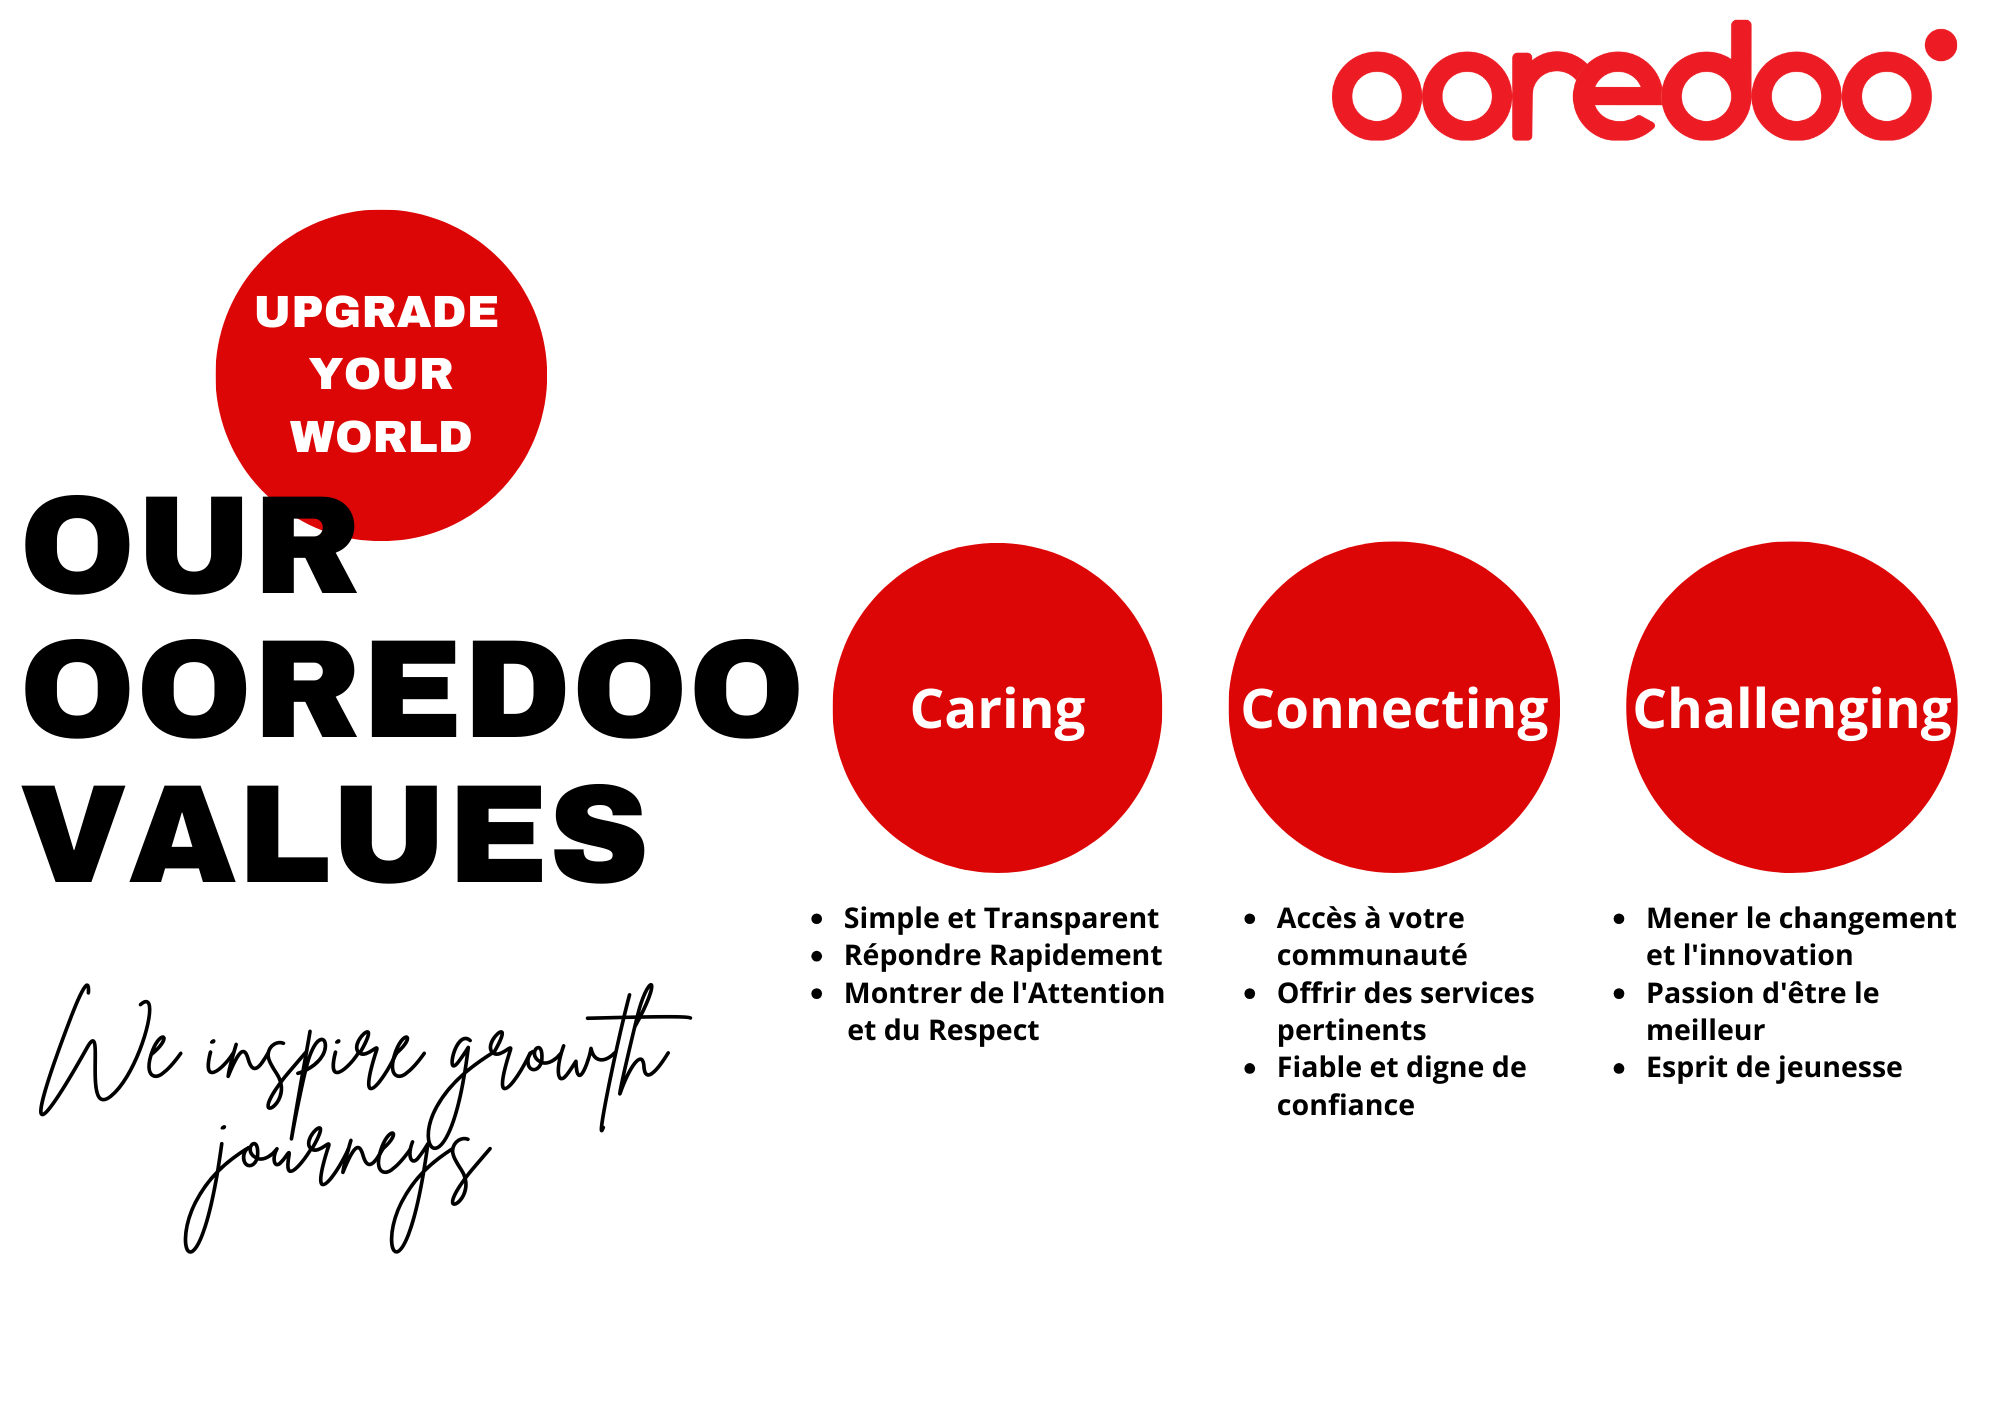
\includegraphics[width=0.6\linewidth]{Value_Ooredoo.png}
    \caption{Récapitulatif des valeurs de l’entreprise}
    \label{valeurs}
\end{figure}

\subsection{La vision de l’entreprise}

 Ooredoo, en tant qu'entreprise résolument orientée vers les besoins des populations, est animée par une vision claire: \textbf{enrichir la vie numérique des gens}. Cette vision repose sur la conviction que la communication est un puissant levier pour stimuler le développement humain et aider les individus à atteindre leurs objectifs, tant personnels que professionnels. 

Ooredoo se donne pour mission de permettre à ses clients d'accéder au meilleur de l'Internet, de manière personnalisée et adaptée à leurs besoins uniques. 

Pour ce faire, l'entreprise continue d'investir dans son réseau Supernet, garantissant des vitesses plus rapides et une connectivité fluide qui répond aux exigences croissantes du monde numérique. 

En tant que véritable facilitateur digital, Ooredoo aspire à simplifier la vie de ses utilisateurs et à leur offrir des expériences numériques enrichissantes et gratifiantes. Prenant les devants dans le domaine des services intelligents, Ooredoo contribue à la construction des « smart cities » et des « smart stadiums » de demain, tout en proposant une riche gamme de services, allant des divertissements numériques à Ooredoo Mobile Money.


\subsection{L’organigramme de l’entreprise} 

 Ooredoo Tunisie compte un effectif total de \textbf{1357 salariés}, comprenant \textbf{838 hommes} et \textbf{519 femmes}.

Le siège se compose de dix directions à savoir: Direction Ressources Humaines, Direction Technologie, Direction Administrative et Financière, Direction Vente et Distribution, Direction Marketing et Direction juridique et régulation.

La figure \ref{Hier} ci-dessous illustre la répartition des principaux postes de direction au sein de l'entreprise.

\begin{figure}[H]
    \centering
    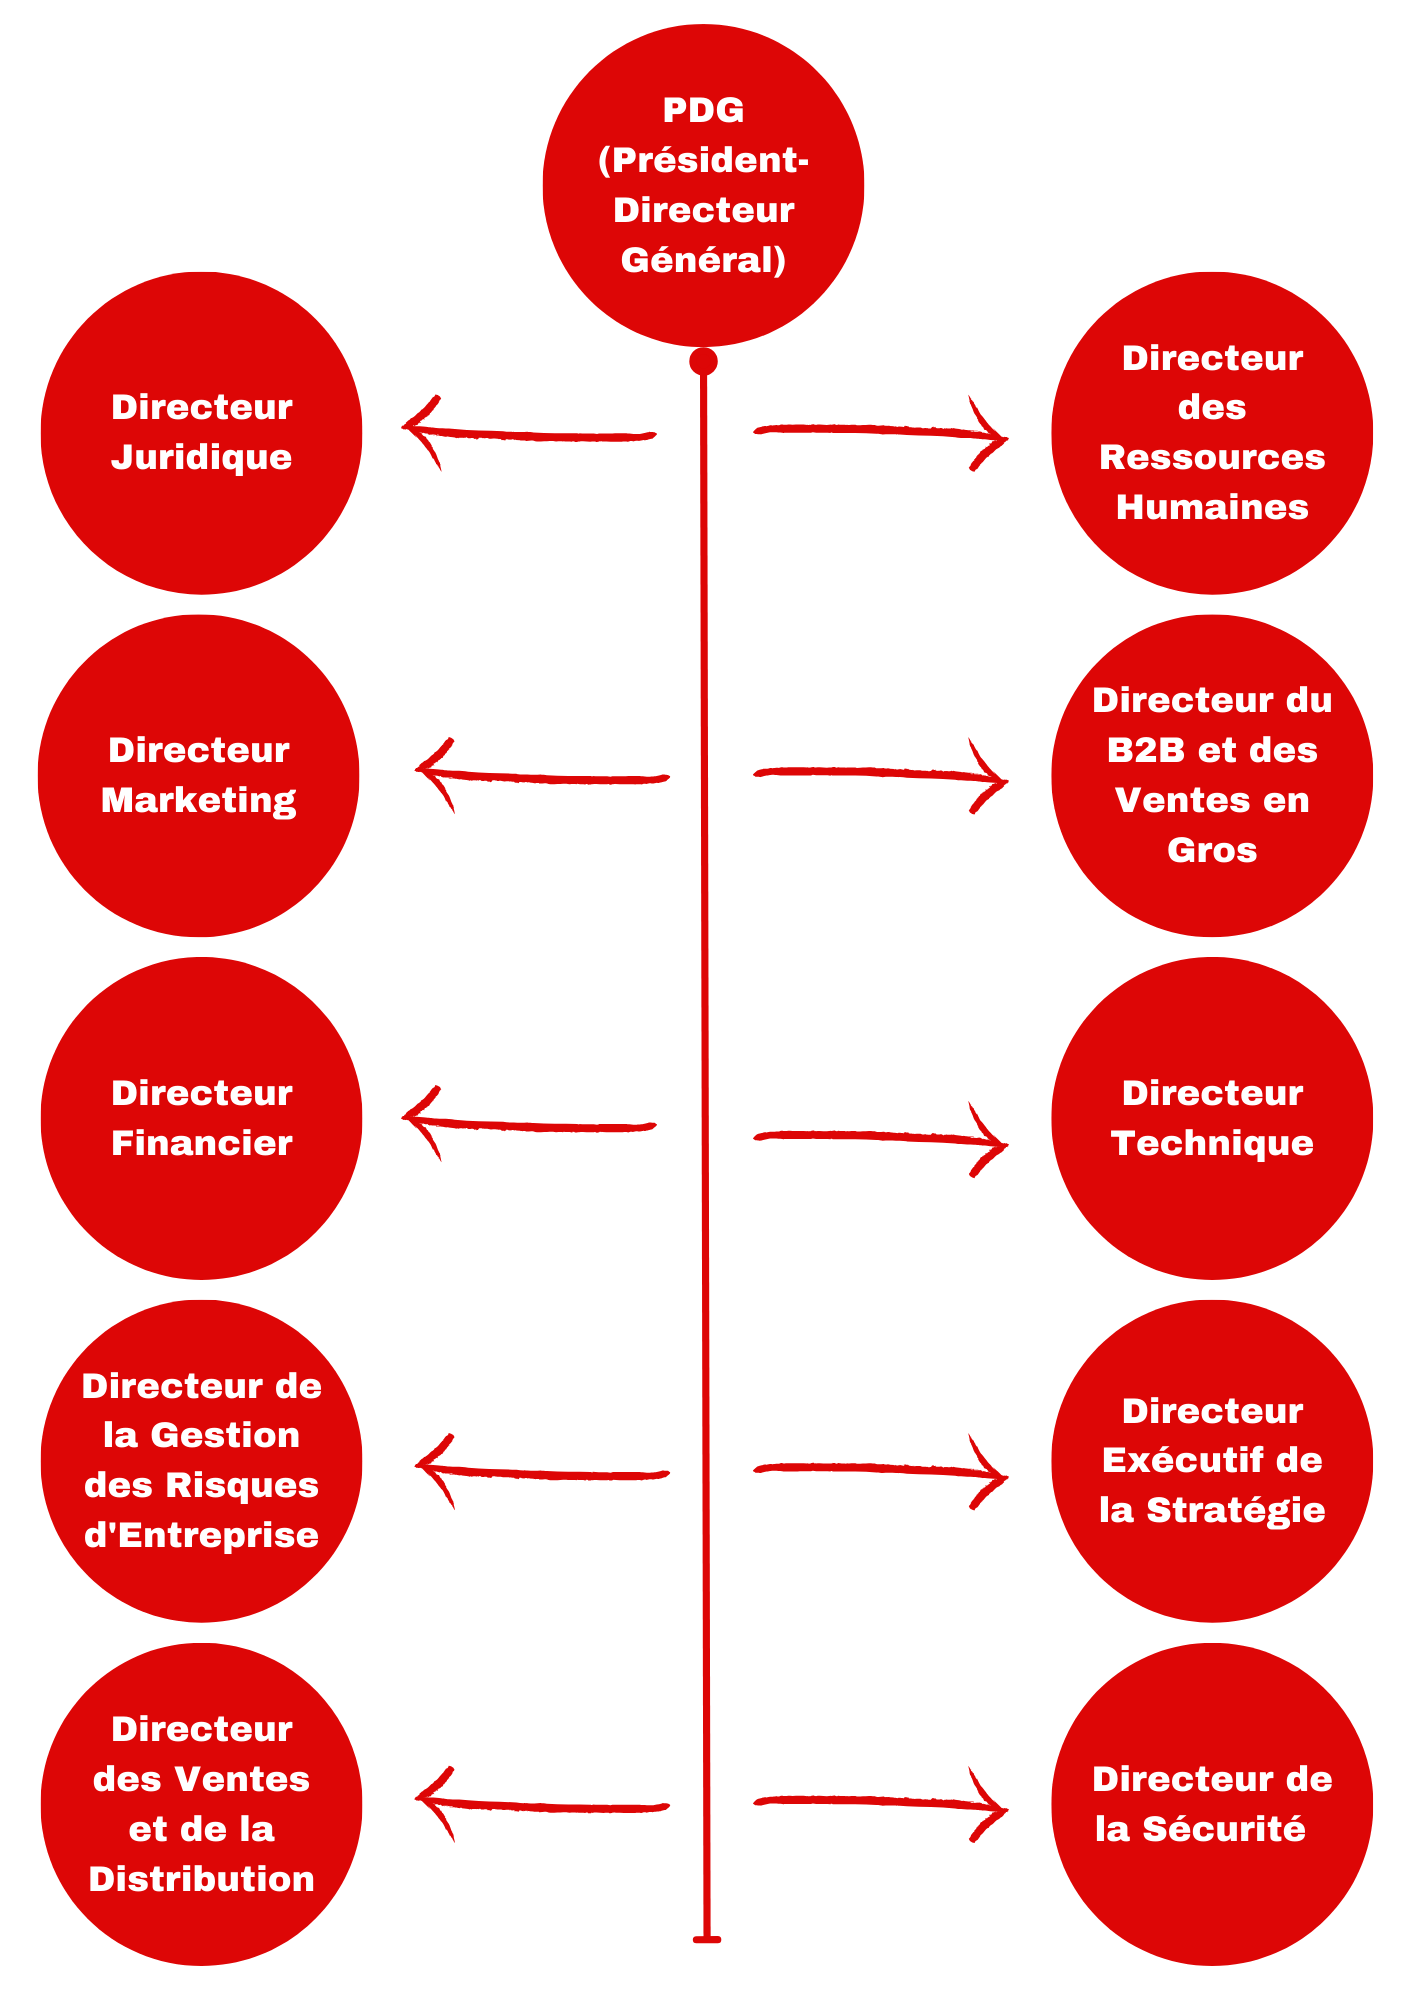
\includegraphics[width=0.5\linewidth]{General_Ooredoo.png}
    \caption{La répartition des principaux postes de direction}
    \label{Hier}
\end{figure}

\subsection{L’organigramme de la direction Technologie }

Au sein de la Direction Technologie chez Ooredoo Tunisie, plusieurs sous-directions jouent un rôle crucial dans la gestion et le développement des infrastructures et des services technologiques. 
La Direction CME (Centre de Maintenance et d'Exploitation) est responsable de la maintenance préventive et corrective des équipements ainsi que de leur exploitation quotidienne pour garantir leur bon fonctionnement. 
\begin{itemize}
    

\item La Direction Support assure l'assistance technique aux utilisateurs internes et externes, gérant les demandes de support et résolvant les problèmes techniques. 
\item La Direction Déploiement et Maintenance se concentre sur l'installation et la configuration des nouvelles solutions technologiques, ainsi que sur la maintenance des systèmes existants. 
\item La Direction Technique est chargée de la gestion des aspects techniques des projets, incluant la conception et l'implémentation de nouvelles technologies. 
\item La Direction Réseau et Service gère l'infrastructure réseau, veillant à la performance et à la sécurité des services de télécommunications. 
\item La Direction Budget, Process et Gestion de Projet supervise la planification budgétaire, les processus internes et le suivi des projets pour assurer leur livraison dans les délais et les coûts impartis.
\item La Direction des Systèmes d'Information (DSI), où se déroule mon stage, est essentielle au sein de la Direction Technologie. Elle s'occupe de la mise en place, du suivi, de la maintenance et de l'optimisation des systèmes informatiques d'Ooredoo. La DSI centralise les données et coordonne des applications clés comme les CRM, ERP, et Data Warehouse, soutenant ainsi les opérations quotidiennes, optimisant les processus internes et facilitant la prise de décision stratégique. Sa gestion est cruciale pour répondre aux besoins croissants en gestion des données et en technologies de l'information.
\end{itemize}
La figure \ref{it} ci-dessous illustre la répartition des différentes directions au sein de la direction Technique.

\begin{figure}[H]
    \centering
    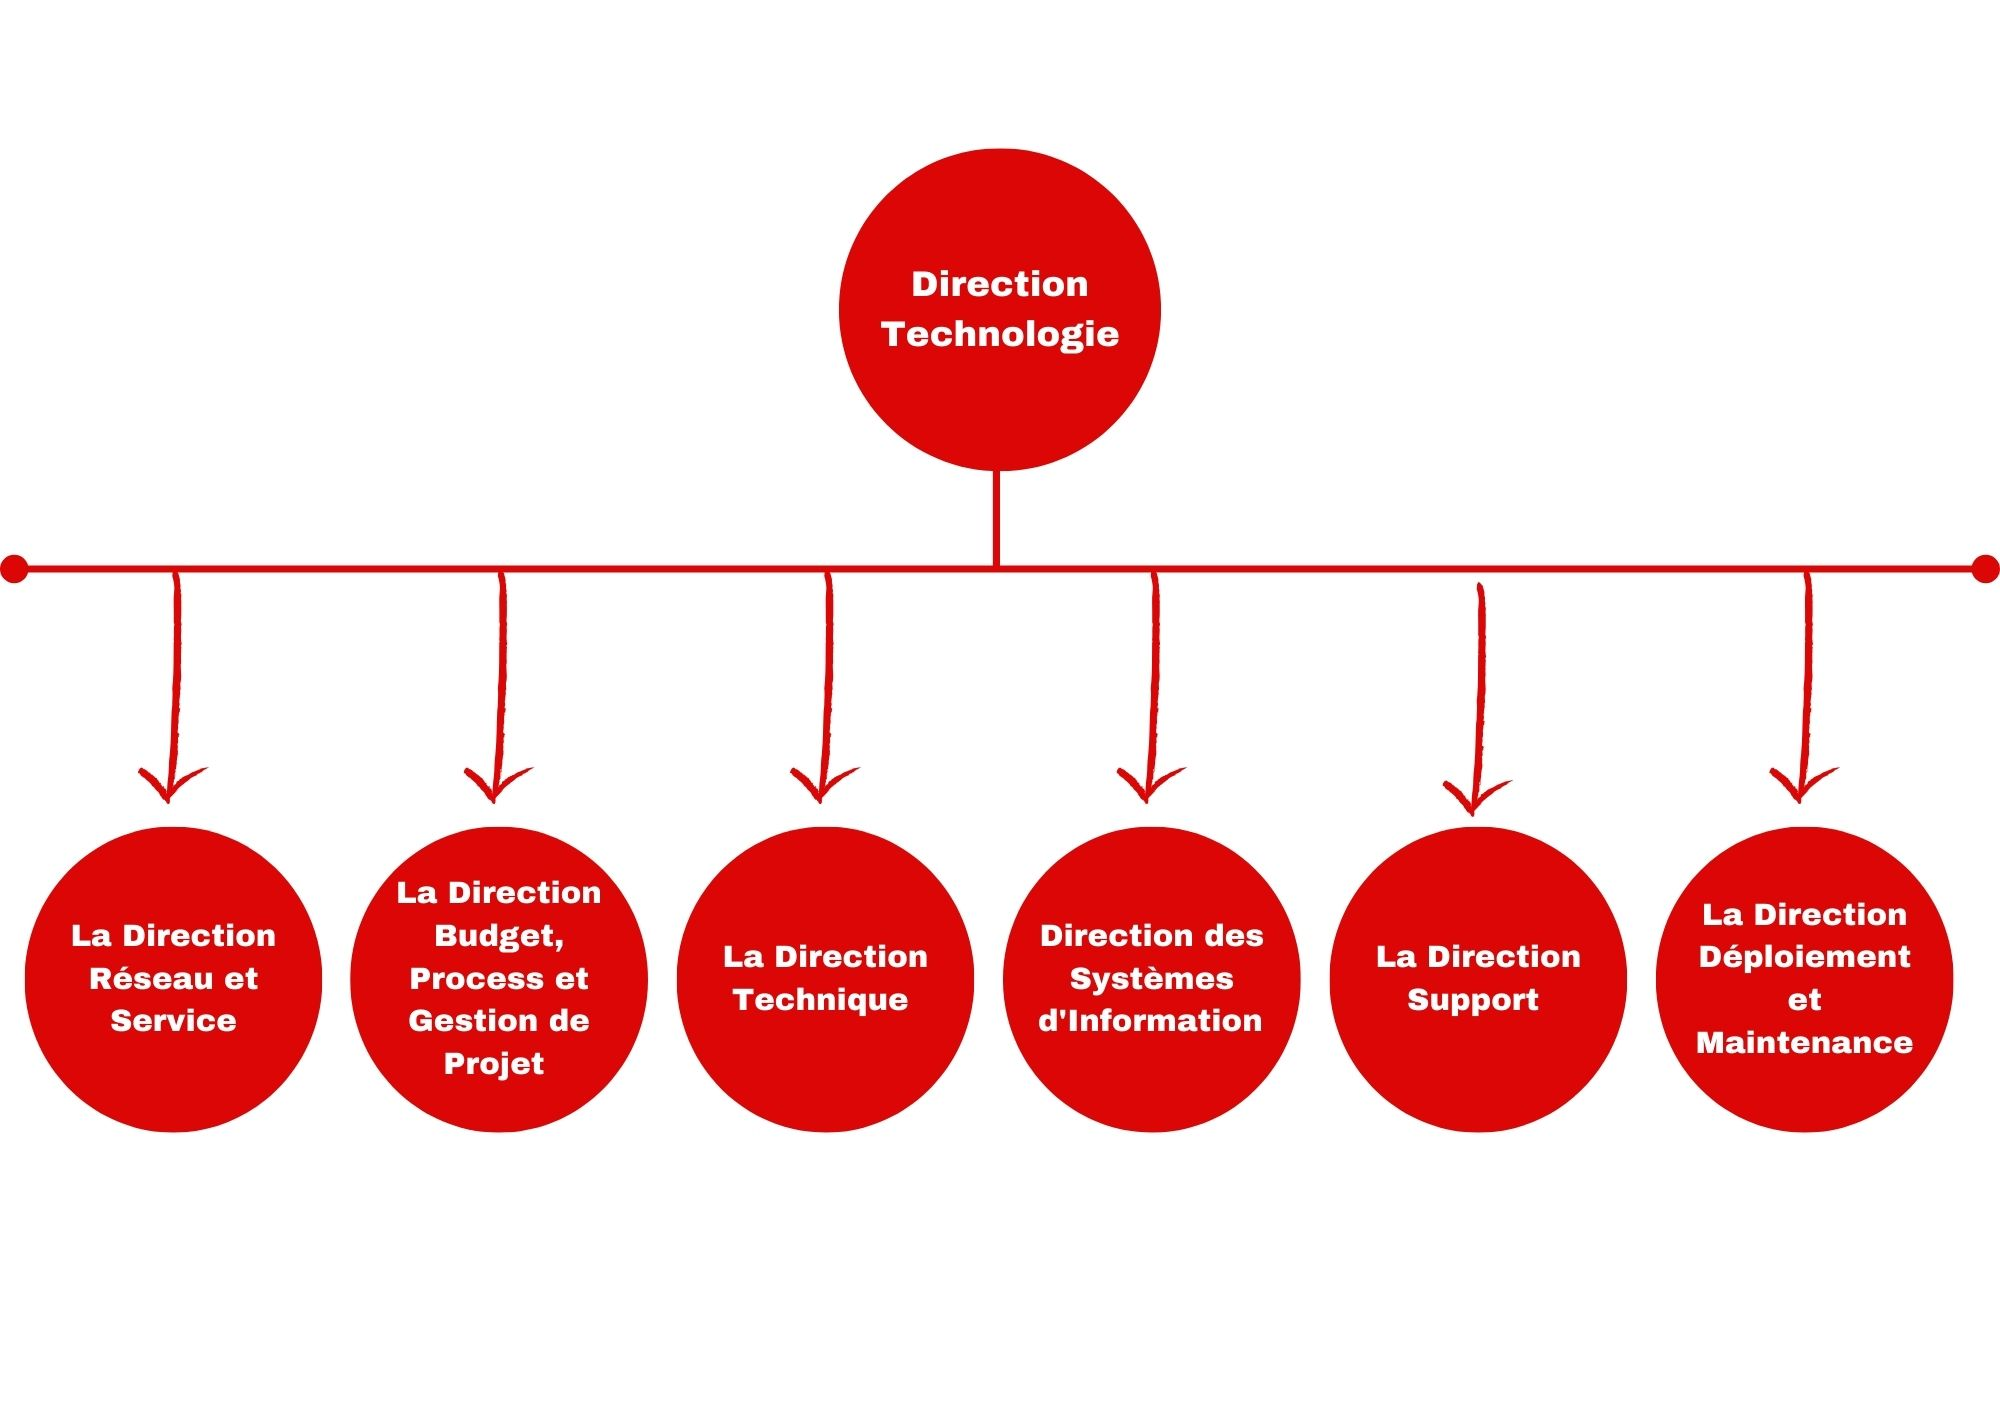
\includegraphics[width=0.5\linewidth]{DepIT_Ooredoo.jpg}
    \caption{Répartition des différentes directions au sein de la direction Technique}
    \label{it}
\end{figure}

\section{Contexte générale du projet}
\subsection{Problématique}

Dans le secteur des télécommunications, la satisfaction des clients est essentielle pour fidéliser la clientèle et se démarquer de la concurrence, notamment face à des acteurs comme Orange et Tunisie Telecom. Les revenus des opérateurs dépendent largement de leur capacité à retenir leurs clients, car l’acquisition de nouveaux clients est souvent plus coûteuse.\par

Comprendre les raisons de la satisfaction ou de l'insatisfaction des clients est donc crucial pour ajuster les stratégies de service et de marketing. Il est important de noter que dans ce secteur, deux types principaux de clients se distinguent : les \textbf{clients prépayés} et les \textbf{clients postpayés}.

\textbf{Clients Prépayés:} Ces clients paient à l'avance pour les services téléphoniques (appels, SMS, données). Leur utilisation dépend fortement de leurs habitudes de consommation et de leur capacité à recharger leur crédit. Ils représentent une catégorie homogène dont le comportement est principalement influencé par la fréquence et le montant de leurs recharges. Par conséquent, les données liées aux recharges, comme \texttt{recharge\_amount} et \texttt{number\_of\_recharges}, sont des indicateurs clés pour comprendre leur satisfaction.

\textbf{Clients Postpayés:} Ces clients, au contraire, paient pour les services utilisés à la fin du mois. Leur consommation est plus stable et moins directement influencée par les recharges. Toutefois, leur comportement est fortement impacté par les offres et promotions auxquelles ils souscrivent, rendant leur analyse plus complexe.

Ces distinctions entre clients prépayés et postpayés sont essentielles pour adapter les analyses et les stratégies de rétention.

En 2022, Tunisie Telecom a enregistré un chiffre d’affaires de 1 288,22 millions de dinars, en hausse de 2,6\% par rapport à 2021. Orange Tunisie a atteint 773,16 millions de dinars, avec une augmentation de 8,8\%. En revanche, Ooredoo Tunisie, qui avait affiché le plus gros chiffre d’affaires du secteur en 2021 avec 1 351,1 millions de dinars, a vu ce chiffre baisser de 0,7\%, s'établissant à 1 306,40 millions de dinars en 2022. Cette situation met en lumière l'importance de mieux comprendre les attentes des clients pour inverser cette tendance.\par

Ooredoo mène des enquêtes mensuelles sur divers aspects tels que la recharge, le réseau, et le retail, pour analyser le comportement des clients au cours des mois précédents. L'objectif est d'identifier les facteurs qui influencent le score de satisfaction (OSAT) et de développer des modèles prédictifs grâce aux techniques de machine learning et de deep learning.\par

En utilisant ces analyses, Ooredoo peut non seulement repérer les clients à risque de départ, mais aussi anticiper leurs besoins pour améliorer leur expérience. Ce projet vise à renforcer la relation client en exploitant les outils avancés de la data science, essentiels pour rester compétitif sur le marché.\par

Pour répondre à cette problématique, ce projet s'efforcera de répondre aux questions suivantes:

\begin{itemize}
    \item Quels sont les principaux facteurs qui influencent la satisfaction des clients ?
    \item Quelles différences de comportement peut-on observer entre les clients satisfaits et insatisfaits, notamment entre les clients prépayés et postpayés ?
    \item Quels modèles de machine learning ou de deep learning offrent les meilleures performances pour prédire la satisfaction générale des clients ?
\end{itemize}

\subsection{Objectif du projet}

L'objectif principal de ce projet est d'explorer et d'analyser les données clients pour comprendre les facteurs influençant leur satisfaction. En se concentrant principalement sur les \textbf{clients prépayés}clients prépayés, ce projet vise à :

\begin{itemize}
    \item \textbf{Identifier les principaux facteurs} qui influencent la satisfaction ou l'insatisfaction des clients.
    \item \textbf{Distinguer les comportements} entre clients satisfaits et insatisfaits en analysant les réponses aux enquêtes et les comportements d’utilisation des services.
    \item \textbf{Développer des modèles prédictifs} utilisant des techniques de machine learning et de deep learning pour prédire avec précision le score de satisfaction (OSAT).
    \item \textbf{Optimiser l’expérience client} en identifiant les segments de clientèle nécessitant des améliorations spécifiques, notamment par une analyse approfondie des clients prépayés.
\end{itemize}

Le projet se déroulera en plusieurs phases : la collecte et le nettoyage des données, l’analyse statistique des résultats, le développement et l’évaluation de modèles prédictifs, ainsi que l'interprétation des résultats pour une application directe dans les stratégies marketing.

\subsection{Méthodologie de travail}

Pour mener à bien ce projet, une approche méthodologique structurée est essentielle. La démarche se décline en plusieurs étapes clés:

\begin{enumerate}
    \item \textbf{Compréhension de la problématique métier}: Cette phase consiste à analyser les enjeux de la satisfaction client dans les télécommunications, à définir les objectifs du projet et à identifier les critères de succès pour Ooredoo Tunisie.
    
    \item \textbf{Compréhension des données}: Cette étape inclut la collecte des données à partir des enquêtes mensuelles d'Ooredoo, suivie de leur nettoyage, transformation et préparation pour garantir leur qualité et pertinence pour l'analyse.
    
    \item \textbf{Analyse des variables}: Cette phase comprend l'exploration des relations entre les variables explicatives et la variable cible (score de satisfaction) en utilisant des techniques telles que la corrélation. Cette analyse permet d'identifier les facteurs influents, leurs interactions et leur impact sur la satisfaction des clients.
    
    \item \textbf{Modélisation}: Nous utilisons divers algorithmes de machine learning et deep learning pour créer des modèles prédictifs. Cette étape vise à développer des modèles capables de prédire avec précision le score de satisfaction des clients.
    
    \item \textbf{Évaluation du modèle}: Après la modélisation, chaque modèle est évalué en termes de performance à l'aide de métriques telles que l'exactitude, la précision, le rappel et le score F1. Cette évaluation permet de sélectionner le modèle le plus performant.
\end{enumerate}

\subsection{Choix technologiques}

Pour réaliser les différentes étapes du projet, plusieurs outils technologiques ont été sélectionnés. Ces outils peuvent être classés en trois catégories: logiciels et environnements de développement, langages de programmation et bibliothèques.

\begin{itemize}
    \item \textbf{Logiciels et environnements de développement}  
    \begin{itemize}
        \item \textbf{SAS Viya}: Une plateforme analytique puissante permettant l'accès aux données, leur manipulation et l'exécution de requêtes complexes en SQL. Utilisée principalement pour manipuler les tables de données et exporter les résultats finaux pour l'analyse.
        \item \textbf{Jupyter Notebook}: Un environnement de développement interactif qui permet de combiner code, texte et visualisations dans un même document, particulièrement adapté pour l'analyse exploratoire des données et la modélisation prédictive.
    \end{itemize}
    
    \item \textbf{Langages de programmation}  
    \begin{itemize}
        \item \textbf{Python}: Langage polyvalent largement utilisé dans l'analyse de données, la modélisation statistique et le machine learning. Il permet de réaliser des tâches complexes grâce à ses bibliothèques variées.
        \item \textbf{SQL}: Langage utilisé pour interagir avec les bases de données relationnelles, permettant d'extraire, manipuler et gérer des ensembles de données.
    \end{itemize}
    
    \item \textbf{Bibliothèques utilisées}  
    \begin{itemize}
        \item \textbf{Numpy}: Bibliothèque fondamentale pour le calcul numérique, permettant de manipuler des tableaux multidimensionnels et de réaliser des opérations mathématiques complexes.
        \item \textbf{Pandas}: Bibliothèque spécialisée dans la manipulation et l'analyse de données, offrant des structures flexibles pour le nettoyage et la transformation des données.
        \item \textbf{Matplotlib}: Bibliothèque de visualisation pour créer des graphiques statiques en 2D.
        \item \textbf{Seaborn}: Basée sur Matplotlib, elle simplifie la création de graphiques statistiques et propose des styles graphiques avancés.
        \item \textbf{Scikit-learn}: Fournit une large gamme d'algorithmes pour la classification, la régression, le clustering et la réduction de dimension.
        \item \textbf{TensorFlow}: Bibliothèque open source pour construire et entraîner des modèles de machine learning, particulièrement des réseaux de neurones.
        \item \textbf{Keras}: Interface de haut niveau pour simplifier la création et la manipulation de réseaux de neurones profonds.
        \item \textbf{PyTorch}: Bibliothèque open source développée par Facebook, populaire pour la recherche en deep learning.
    \end{itemize}
\end{itemize}

\section{Concepts Clés}
L'ère numérique a révolutionné l'exploitation des données. Dans ce contexte, le Machine Learning, le Data Mining et le Deep Learning jouent un rôle clé pour analyser les données massives et en extraire des insights significatifs. 

Le Data Mining permet d'explorer et de découvrir des modèles dans les données, tandis que le Machine Learning utilise ces insights pour construire des modèles prédictifs. Enfin, le Deep Learning, en tant que sous-domaine du Machine Learning, emploie des réseaux de neurones profonds pour traiter des données non structurées et capturer des relations complexes.

Cette section abordera chacun de ces concepts, en soulignant leur définition et leur application dans le projet de prédiction de la satisfaction client.

\subsection{Data Mining}

Le \textbf{Data Mining}, ou fouille de données, est le processus d'analyse de grandes quantités de données pour découvrir des informations utiles, des tendances cachées, ou des relations insoupçonnées. Utilisé dans divers secteurs comme le marketing, la santé, ou l'éducation, il permet aux entreprises de mieux comprendre leurs clients et d'optimiser leurs stratégies en fonction des comportements observés.

Contrairement à d'autres approches, le Data Mining est davantage orienté vers l'analyse exploratoire des données. Il se concentre principalement sur la découverte de connaissances à partir des données disponibles, sans qu'il y ait nécessairement une phase de prédiction.

Les principales étapes du processus de Data Mining sont les suivantes:

\begin{itemize}
    \item \textbf{Collecte des données}: Rassemblement d'informations à partir de diverses sources, telles que des bases de données ou des fichiers.
    \item \textbf{Préparation des données}: Nettoyage et transformation des données afin d'assurer leur qualité, en supprimant les erreurs, en gérant les valeurs manquantes, et en normalisant les variables. Cette phase inclut également des techniques comme le \textbf{clustering} pour regrouper les données en sous-ensembles homogènes, facilitant ainsi leur analyse. Dans certains cas, des méthodes comme \textbf{SMOTE} (Synthetic Minority Over-sampling Technique) peuvent être utilisées pour rééquilibrer les jeux de données déséquilibrés.
    \item \textbf{Exploration des données}: Utilisation d'outils statistiques et analytiques pour identifier des tendances, des motifs ou des anomalies.
\end{itemize}

Le Data Mining utilise plusieurs techniques clés, telles que le clustering et la classification, pour faciliter l'exploration des données. Cependant, son objectif est principalement descriptif, contrairement à des techniques prédictives comme celles employées en Machine Learning. Le Data Mining permet ainsi de mieux comprendre les données, de découvrir des corrélations et d'aider à la prise de décisions éclairées.

\subsection{Machine Learning}

Le \textbf{Machine Learning}, ou apprentissage automatique, est une branche de l'intelligence artificielle (IA) qui permet aux machines d'apprendre à partir de données sans être explicitement programmées pour chaque tâche. Contrairement au Data Mining, le Machine Learning est principalement orienté vers la prédiction et l'automatisation de tâches à partir de modèles qui apprennent continuellement à partir des données.

Il existe trois principaux types de Machine Learning:

\begin{itemize}
    \item \textbf{Apprentissage supervisé}: Le modèle apprend à partir de données étiquetées, où les entrées sont associées à des sorties connues. Exemple: prédire la satisfaction des clients en fonction de caractéristiques passées.
    \item \textbf{Apprentissage non supervisé}: Le modèle identifie des structures cachées dans les données non étiquetées. Exemple: regrouper des clients en fonction de comportements similaires via le \textbf{clustering}.
    \item \textbf{Apprentissage par renforcement}: Le modèle interagit avec un environnement et apprend à partir des récompenses ou pénalités qu'il reçoit. Cette approche est souvent utilisée dans des applications comme la robotique ou les jeux vidéo.
\end{itemize}

Le Machine Learning se distingue du Data Mining par son caractère itératif et automatisé. Une fois que le modèle est entraîné, il peut faire des prédictions sur de nouvelles données et s'améliorer au fil du temps. Le processus typique de Machine Learning comprend les étapes suivantes:

\begin{itemize}
    \item \textbf{Sélection des caractéristiques}: Choix des variables pertinentes pour l'entraînement des modèles.
    \item \textbf{Choix des algorithmes}: En fonction des objectifs, différents algorithmes comme la \textbf{régression logistique}, les \textbf{forêts aléatoires} ou les \textbf{SVM} sont utilisés.
    \item \textbf{Entraînement du modèle}: Le modèle est ajusté à l'aide de données d'entraînement pour minimiser l'erreur entre les prédictions et les résultats réels.
    \item \textbf{Évaluation et optimisation}: Le modèle est évalué et amélioré à l'aide de techniques comme la validation croisée et l'optimisation des hyperparamètres.
\end{itemize}

\subsection{Data Mining vs Machine Learning}

Bien que le \textbf{Data Mining} et le \textbf{Machine Learning} partagent certains outils et objectifs, comme l'exploration des données pour en extraire des informations utiles, ils se distinguent par leurs approches et leurs finalités:

\begin{itemize}
    \item Le \textbf{Data Mining} est principalement orienté vers l'exploration et la compréhension des données historiques à l'aide de techniques descriptives. Il est souvent utilisé pour découvrir des modèles et des relations au sein des données.
    \item Le \textbf{Machine Learning}, quant à lui, adopte une approche prédictive et automatisée. Il vise à créer des modèles capables de généraliser à de nouvelles données pour prédire des résultats futurs.
    \item Dans le Data Mining, les techniques comme la \textbf{classification} et le \textbf{clustering} sont utilisées pour segmenter les données et en extraire des connaissances. En Machine Learning, ces mêmes techniques sont utilisées pour construire des modèles prédictifs qui évoluent au fil du temps.
\end{itemize}


En somme, bien que complémentaires, le Data Mining et le Machine Learning diffèrent dans leurs applications. Le Data Mining s'attache à décrire et analyser les données existantes, tandis que le Machine Learning se concentre sur l'automatisation et la prédiction, permettant de prendre des décisions ou d'effectuer des tâches complexes à grande échelle.

\subsection{Deep Learning}

Le \textbf{Deep Learning} est une branche spécifique du Machine Learning qui repose sur l'utilisation de réseaux de neurones artificiels. Contrairement aux algorithmes de Machine Learning traditionnels, les modèles de Deep Learning peuvent apprendre à partir de grandes quantités de données non structurées et extraire automatiquement des caractéristiques complexes sans intervention humaine. 

Ce processus est particulièrement efficace dans des domaines comme la reconnaissance d'images, le traitement du langage naturel, et l'analyse vocale, où les données sont volumineuses et hétérogènes.

Les réseaux de neurones artificiels utilisés en Deep Learning sont composés de plusieurs couches d'unités (ou neurones) qui sont interconnectées. Les modèles les plus communs sont les réseaux de neurones à propagation avant (feedforward) et les réseaux de neurones convolutifs (CNN) pour les images.

\subsubsection{Principes du Deep Learning}

Le Deep Learning se distingue par sa capacité à apprendre des représentations complexes à travers les couches hiérarchiques des réseaux de neurones:

\begin{itemize}
    \item \textbf{Les couches de neurones}: Un réseau de neurones profond est composé de plusieurs couches successives. Chaque couche transforme les données reçues, en extrayant des caractéristiques de plus en plus abstraites.
    \item \textbf{Fonctions d'activation}: Chaque neurone applique une fonction d'activation (comme \textbf{ReLU}, \textbf{sigmoïde} ou \textbf{tanh}) pour introduire de la non-linéarité dans le modèle, ce qui lui permet d'apprendre des relations complexes dans les données.
    \item \textbf{Entraînement par rétropropagation}: Les réseaux de neurones sont entraînés à l'aide d'une technique appelée \textbf{backpropagation}, qui ajuste les poids des connexions entre les neurones en minimisant une fonction de coût via la descente de gradient.
    \item \textbf{Régularisation et Dropout}: Pour éviter le sur-apprentissage (overfitting), des techniques comme la régularisation L2 ou le \textbf{dropout} sont utilisées. Le dropout consiste à désactiver aléatoirement des neurones pendant l'entraînement pour améliorer la généralisation.
\end{itemize}

\subsubsection{Applications du Deep Learning}

Le Deep Learning est particulièrement adapté pour les tâches impliquant de grandes quantités de données non structurées. Voici quelques exemples d'applications:

\begin{itemize}
    \item \textbf{Reconnaissance d'images}: Utilisation de réseaux de neurones convolutifs (CNN) pour l'identification d'objets, de visages, ou de scènes dans les images.
    \item \textbf{Traitement du langage naturel (NLP)}: Utilisation de modèles comme les \textbf{réseaux de neurones récurrents (RNN)} ou les \textbf{transformers} pour la traduction automatique, la génération de texte, ou l'analyse de sentiments.
    \item \textbf{Analyse vocale}: Reconnaissance vocale automatisée via des réseaux profonds pour transformer les signaux audio en texte ou en commandes.
\end{itemize}

\subsubsection{Différence entre Machine Learning et Deep Learning}

Bien que le Deep Learning soit une sous-catégorie du Machine Learning, il se distingue par sa capacité à gérer des quantités massives de données et par sa structure en couches profondes. Contrairement aux algorithmes traditionnels de Machine Learning, où les caractéristiques doivent souvent être définies manuellement, le Deep Learning apprend automatiquement à extraire des caractéristiques complexes à partir des données brutes.

Voici quelques différences principales:
\begin{itemize}
    \item \textbf{Caractéristiques automatiques}: Dans le Machine Learning traditionnel, les ingénieurs doivent sélectionner manuellement les caractéristiques les plus pertinentes. En Deep Learning, les modèles apprennent directement à extraire les meilleures caractéristiques des données brutes.
    \item \textbf{Quantité de données}: Le Deep Learning nécessite généralement beaucoup plus de données pour fonctionner efficacement, alors que les algorithmes de Machine Learning traditionnels peuvent être appliqués à des ensembles de données plus petits.
    \item \textbf{Complexité des modèles}: Les modèles de Deep Learning, composés de nombreuses couches de neurones, sont bien plus complexes et peuvent capturer des relations non linéaires plus profondes que les modèles de Machine Learning classiques.
\end{itemize}

Ainsi, le Deep Learning permet de traiter des problèmes complexes nécessitant un apprentissage à partir de données massives et non structurées, offrant des performances exceptionnelles dans des domaines comme la vision par ordinateur et le traitement du langage naturel.

\section{Conclusion}
Ce chapitre a posé les bases nécessaires à la compréhension du projet en détaillant son contexte, ses objectifs, et les concepts théoriques associés. Les éléments présentés permettront de mieux appréhender les étapes suivantes de l'analyse et de la modélisation des données dans les prochains chapitres.


% \chapter{Outils mathématiques d'ordre général}
\begin{spacing}{1.2}
\minitoc
\thispagestyle{MyStyle}
% \setstretch{1.2} 
\end{spacing}
\newpage
\justifying

\sloppy \setstretch{1.3} 
\section{Introduction}

Ce chapitre couvre les techniques de prétraitement, les tests de corrélation et la modélisation. Nous abordons des méthodes comme la normalisation et le traitement des valeurs manquantes, puis explorons des outils statistiques pour analyser les relations entre variables. Enfin, nous présentons des techniques de modélisation, incluant l’équilibrage des classes et la sélection de caractéristiques, qui améliorent les performances des modèles prédictifs.

\section{Techniques de Prétraitement des Données}

Le prétraitement des données est une étape cruciale pour améliorer la qualité des données et optimiser les performances des modèles. Il inclut des méthodes comme la normalisation, qui ajuste l'échelle des variables, et le traitement des valeurs manquantes.

\subsection{Normalisation des Données}

La normalisation met toutes les variables sur une même échelle, ce qui est essentiel pour éviter qu'une variable domine en raison de son amplitude. C’est particulièrement utile pour les algorithmes sensibles à l'échelle des données.

\subsubsection{Méthodes classiques de normalisation}

\textbf{\(\checkmark\)} \textbf{Normalisation Min-Max} \\
Elle met les données à l’échelle entre 0 et 1 selon la formule suivante: 
    \[
    X_{\text{norm}} = \frac{X - X_{\text{min}}}{X_{\text{max}} - X_{\text{min}}}
    \]
\textbf{\(\rightarrow\)} \textbf{Utilité}: Recommandée pour les algorithmes comme les réseaux de neurones.\\
\textbf{\(\rightarrow\)} \textbf{Impact}: Sensible aux valeurs extrêmes (outliers).

\textbf{\(\checkmark\)} \textbf{Z-Score (Standardisation)} \\
    Cette méthode centre les données à 0 avec un écart-type de 1 selon la formule suivante:
    \[
    X_{\text{std}} = \frac{X - \mu}{\sigma}
    \]
\textbf{\(\rightarrow\)} \textbf{Utilité}: Utile pour ajuster les échelles sans affecter la structure des variables, peu importe la distribution.\\
\textbf{\(\rightarrow\)} \textbf{Impact}: Uniformise l'effet des variables sur le modèle.

\textbf{\(\checkmark\)} \textbf{Normalisation Logarithmique (Log)} \\
    La transformation logarithmique réduit l'influence des grandes valeurs et rend les distributions plus symétriques selon la formule suivante: 
    \[
    X_{\text{log}} = \log(X + 1)
    \]
\textbf{\(\rightarrow\)} \textbf{Utilité}: Efficace pour réduire les écarts dus aux valeurs extrêmes.\\
\textbf{\(\rightarrow\)} \textbf{Impact}: Diminue l'influence des grandes valeurs.

\textbf{\(\checkmark\)} \textbf{Transformation par Racine Carrée (Sqrt)} \\
    Cette transformation réduit la variance tout en préservant la hiérarchie des données. Formule :
    \[
    X_{\text{sqrt}} = \sqrt{X}
    \]
\textbf{\(\rightarrow\)} \textbf{Utilité}: Réduit l'impact des grandes valeurs sans affecter l'ordre des données.\\
\textbf{\(\rightarrow\)} \textbf{Impact}: Atténue les grandes variations tout en maintenant la structure des données.

\subsubsection{Méthodes avancées de normalisation}

Pour améliorer la qualité des données, surtout lorsque celles-ci ne suivent pas une distribution normale, des techniques avancées comme la transformation de Box-Cox et la transformation de Yeo-Johnson sont souvent employées.

\textbf{\(\checkmark\)} \textbf{Transformation de Box-Cox} \\
La transformation de Box-Cox \cite{titleB1000} stabilise la variance et rapproche les données d'une distribution normale. Elle est définie par:

\[
y(\lambda) =
\begin{cases} 
\frac{x^\lambda - 1}{\lambda}, & \text{si } \lambda \neq 0 \\
\log(x), & \text{si } \lambda = 0
\end{cases}
\]

\noindent \textbf{\(\rightarrow\)} \textbf{Explication}: Box-Cox applique une transformation exponentielle ou logarithmique aux données, selon la valeur de $\lambda$. Lorsque $\lambda$ est différent de zéro, la transformation lisse les données et réduit l'asymétrie en modifiant la relation entre les valeurs observées et la moyenne. Si $\lambda = 0$, elle applique une transformation logarithmique pour atténuer l'impact des grandes valeurs tout en rendant la distribution plus symétrique. Nous approfondirons la notion de \textbf{log-vraisemblance} dans une section ultérieure.\\
\textbf{\(\rightarrow\)} \textbf{Utilité}: Utile pour les données strictement positives, permet d'uniformiser les distributions non normales.\\
\textbf{\(\rightarrow\)} \textbf{Choix de $\lambda$}: Le paramètre $\lambda$ est choisi par maximisation de la log-vraisemblance.

\textbf{\(\checkmark\)} \textbf{Transformation de Yeo-Johnson} \\
La transformation de Yeo-Johnson \cite{haha} est une généralisation de Box-Cox qui permet de traiter à la fois les données positives et négatives. Elle est définie par:

\[
y(\lambda) =
\begin{cases} 
\frac{(x + 1)^\lambda - 1}{\lambda}, & \text{si } \lambda \neq 0 \text{ et } x \geq 0 \\
\log(x + 1), & \text{si } \lambda = 0 \text{ et } x \geq 0 \\
-\frac{(-x + 1)^{2 - \lambda} - 1}{2 - \lambda}, & \text{si } \lambda \neq 2 \text{ et } x < 0 \\
-\log(-x + 1), & \text{si } \lambda = 2 \text{ et } x < 0
\end{cases}
\]

\noindent \textbf{\(\rightarrow\)} \textbf{Utilité}: Permet de traiter les données négatives et positives, rendant les données plus normalisées.\\
\textbf{\(\rightarrow\)} \textbf{Choix de $\lambda$}: Comme pour Box-Cox, $\lambda$ est déterminé par maximisation de la log-vraisemblance.

\subsection{Traitement des Valeurs Manquantes}

Le traitement des valeurs manquantes est crucial pour maintenir la qualité des modèles prédictifs. Il permet d'éviter les biais introduits par des données incomplètes en remplaçant les valeurs manquantes par des estimations appropriées.

\subsubsection{Imputation par la Médiane}

L’imputation par la médiane est une méthode simple qui remplace les valeurs manquantes par la médiane de la variable concernée. Elle est particulièrement efficace pour les données avec des valeurs extrêmes (outliers), car la médiane n'est pas influencée par ces dernières.

\[
x_{i,\text{missing}} = \text{Médiane}(x_i)
\]

\noindent \textbf{\(\rightarrow\)} \textbf{Utilité}: Adaptée aux distributions asymétriques.\\
\textbf{\(\rightarrow\)} \textbf{Impact}: Remplace les valeurs manquantes sans perturber la distribution des données.

\subsubsection{K-Nearest Neighbors pour la Prédiction des Valeurs Manquantes}

Le K-Nearest Neighbors (KNN) repose sur la similarité des données pour imputer les valeurs manquantes. Il identifie les \(k\) voisins les plus proches de l'observation avec la valeur manquante, en se basant sur une mesure de distance. Parmi ces mesures, la distance de Minkowski est une généralisation couramment utilisée.

\textbf{\(\checkmark\)} \textbf{Étape 1: Calcul de la distance de Minkowski:} \\
La distance de Minkowski \cite{min} est définie par :

\[
d(x_i, x_j) = \left( \sum_{k=1}^{n} |x_{ik} - x_{jk}|^p \right)^{1/p}
\]

\textbf{Cas particuliers:}\\
\textbf{\(\rightarrow\)} Si \( p = 2 \), on obtient la \textbf{distance euclidienne} \cite{euc}, utilisée pour les données continues.\\
\textbf{\(\rightarrow\)} Si \( p = 1 \), on obtient la \textbf{distance de Manhattan}, adaptée aux données avec de grandes variations.\\
\textbf{\(\rightarrow\)} Pour d'autres valeurs de \( p \), la \textbf{distance de Minkowski} offre une flexibilité accrue pour ajuster la mesure de similarité.

\noindent \textbf{\(\rightarrow\)} \textbf{Utilité}: Chaque type de distance est choisi en fonction de la nature des données.\\
\textbf{\(\rightarrow\)} \textbf{Impact}: Le choix de la distance influence les voisins sélectionnés, et donc la précision de l'imputation.

\textbf{\(\checkmark\)} \textbf{Étape 2: Moyenne pondérée des voisins:} \\
Une fois les voisins identifiés, la valeur manquante est imputée par une moyenne pondérée de leurs valeurs :

\[
x_{i,\text{missing}} = \frac{\sum_{j \in N(i)} w_j x_j}{\sum_{j \in N(i)} w_j}
\]

où \(w_j\) est un poids inversement proportionnel à la distance \(d(x_i, x_j)\).

\noindent \textbf{\(\rightarrow\)} \textbf{Utilité}: Produit des estimations plus précises que les méthodes simples.\\
\textbf{\(\rightarrow\)} \textbf{Impact}: Les valeurs imputées sont souvent plus proches des vraies données manquantes, augmentant la précision des modèles.

\subsection{Conclusion}

Le prétraitement, notamment la normalisation et le traitement des valeurs manquantes, est essentiel pour garantir des données comparables et fiables, améliorant ainsi les performances des modèles prédictifs.

\section{Les indicateurs statistiques}

Les \textbf{indicateurs statistiques} résument les données et permettent de mesurer les relations entre variables. Parmi eux, on trouve:\\

\noindent  \textbf{\(\rightarrow\)} \textbf{Tendance centrale :} Moyenne, médiane, mode indiquent où se concentrent les valeurs.\\
\textbf{\(\rightarrow\)} \textbf{Dispersion :} Variance, écart-type et étendue quantifient la variabilité autour de la tendance centrale.\\
\textbf{\(\rightarrow\)} \textbf{Relation :} Covariance et coefficient de corrélation mesurent les relations linéaires entre variables quantitatives.\\
\textbf{\(\rightarrow\)} \textbf{Association :} L’Eta carré et le Cramer V évaluent l’association entre variables.

\subsection{Eta Carré}

L'Eta carré (\(\eta^2\)) quantifie la part de variance d'une variable quantitative expliquée par une variable qualitative. Il mesure l'effet d'un facteur.

\[
\eta^2 = \frac{SSB}{SSB + SSW}
\]

Avec :
\begin{itemize}
    \item \( SSB \) : Somme des Carrés Entre les Groupes, mesurant la différence entre les moyennes des groupes et la moyenne générale.
    \item \( SSW \) : Somme des Carrés Intra-Groupes, mesurant la variabilité à l'intérieur de chaque groupe.
\end{itemize}

\textbf{\(\checkmark\)} \textbf{Interprétation}:\\
\noindent \textbf{\(\rightarrow\)} \(\eta^2 \leq 0.01\) : Effet faible.\\
\textbf{\(\rightarrow\)} \(0.01 < \eta^2 \leq 0.06\) : Effet modéré.\\
\textbf{\(\rightarrow\)} \(\eta^2 > 0.06\) : Effet fort.

\subsection{Cramer V}

Le \textbf{Cramer V} mesure la force de l'association entre deux variables qualitatives, basé sur la statistique du \(\chi^2\). Il est souvent utilisé avec un \textbf{tableau de contingence}, qui montre la fréquence des combinaisons possibles entre deux variables catégorielles. On détaillera ce tableau et le calcul du \(\chi^2\) dans une prochaine section.

\[
V = \sqrt{\frac{X^2}{N \times \min(k-1, r-1)}}
\]

Où:
\begin{itemize}
    \item \(X^2\) est la statistique du \(\chi^2\),
    \item \(N\) est le nombre total d’observations,
    \item \(k\) et \(r\) sont respectivement le nombre de colonnes et de lignes dans le tableau de contingence.
\end{itemize}

\textbf{\(\checkmark\)} \textbf{Interprétation}: \\
\noindent \textbf{\(\rightarrow\)} $V \leq 0.10$: Association faible.\\
\textbf{\(\rightarrow\)} $0.10 < V \leq 0.30$: Association modérée.\\
\textbf{\(\rightarrow\)} $V > 0.30$: Forte association.

\subsection{Lambda de Goodman et Kruskal}

Le \textbf{Lambda} (\(\lambda\)) de Goodman et Kruskal \cite{gm} mesure l'amélioration de la prédiction d'une variable qualitative dépendante en fonction d'une variable qualitative indépendante. Il compare les erreurs de prédiction avec et sans la variable indépendante.
\[
\lambda = \frac{E_0 - E_1}{E_0}
\]

Où:
\begin{itemize}
    \item \(E_0 = N - \max_j(n_j)\) est le nombre d'erreurs si l'on prédit toujours la modalité la plus fréquente de la variable dépendante (erreurs sans utiliser la variable indépendante),
    \item \(E_1 = \sum_{i} \left( n_i - \max_j \left( n_{ij} \right) \right)\) est le nombre d'erreurs en utilisant la variable indépendante pour prédire la variable dépendante.
\end{itemize}

\textbf{\(\checkmark\)} \textbf{Interprétation}:\\
\noindent \textbf{\(\rightarrow\)} \( \lambda \leq 0.10 \): Amélioration faible.\\
\textbf{\(\rightarrow\)}  \( 0.10 < \lambda \leq 0.30 \): Amélioration modérée.\\
\textbf{\(\rightarrow\)}  \( \lambda > 0.30 \): Amélioration significative.

\subsection{Covariance}

La \textbf{covariance} mesure la variation conjointe de deux variables quantitatives, indiquant si elles augmentent ou diminuent ensemble. Elle est calculée par la somme des produits des écarts par rapport à leurs moyennes:

\[
\text{Cov}(X, Y) = \frac{1}{N} \sum_{i=1}^{N} (X_i - \bar{X})(Y_i - \bar{Y})
\]

Où:
\begin{itemize}
    \item \(X_i\) et \(Y_i\) sont les valeurs des variables pour l’observation \(i\),
    \item \(\bar{X}\) et \(\bar{Y}\) sont les moyennes des variables \(X\) et \(Y\),
    \item \(N\) est le nombre d'observations.
\end{itemize}

\textbf{\(\checkmark\)} \textbf{Interprétation}:\\
\noindent \textbf{\(\rightarrow\)} Covariance positive: Les variables augmentent ensemble.\\
\textbf{\(\rightarrow\)} Covariance proche de zéro: Relation faible.\\
\textbf{\(\rightarrow\)} Covariance négative: Quand une variable augmente, l'autre diminue.

\subsection{Limitation des Indicateurs Statistiques}

\begin{itemize}
    \item \textbf{Cramer V:} Sensible à la taille de l'échantillon.
    \item \textbf{Covariance:} Dépendante des unités de mesure.
    \item \textbf{Goodman et Kruskal Lambda:} Insensible aux petites variations.
    \item \textbf{Eta Carré:} Ne mesure que la force de l'association.
\end{itemize}

\subsection{Conclusion}

En résumé, les indicateurs comme le Cramer V, le Lambda de Goodman et Kruskal, la covariance et l'Eta carré permettent d'analyser les relations entre variables. Cependant, leurs limites, telles que la sensibilité à l'échelle des données et à la taille de l'échantillon, doivent être considérées pour garantir une interprétation fiable.

\section{Les Tests de corrélation}

 Les tests de corrélation évaluent la relation entre deux variables. Ils se divisent en tests paramétriques, comme Pearson \cite{pearson} et ANOVA, qui supposent la normalité des données, et en tests non paramétriques, comme Mann-Whitney \cite{U} et Spearman, qui sont plus flexibles en l'absence de ces conditions.

\subsection*{Types de Corrélation}

\begin{itemize}
 \item \textbf{Corrélation Positive}: Les deux variables augmentent ou diminuent ensemble.
 \item \textbf{Corrélation Négative}: L'augmentation d'une variable entraîne la diminution de l'autre.
 \item \textbf{Corrélation Nulle}: Aucune relation linéaire apparente entre les variables.
\end{itemize}

\subsection*{Limites de la Corrélation} 

La corrélation est sensible aux valeurs aberrantes, ne traite que les relations linéaires et ne détecte pas les relations complexes.

\subsection{Tests paramétriques}

Les tests paramétriques, plus puissants que les non-paramétriques, détectent mieux les effets réels et augmentent la probabilité de rejeter l'hypothèse nulle (H0) lorsqu'une différence existe, surtout lorsque les conditions sont respectées, conduisant souvent à une p-value plus faible.
\subsubsection{Les conditions pour appliquer les tests paramétriques}
\subsubsection*{Vérification de la normalité des données:}

La vérification de la normalité est essentielle avant d'appliquer des tests paramétriques. Le test de Shapiro-Wilk \cite{11} utilise la statistique \( W \) pour évaluer si un échantillon suit une loi normale. Si la p-value associée à \( W \) est inférieure à 0,05, l'hypothèse de normalité est rejetée.

\textbf{\(\checkmark\)} \textbf{Hypothèses du Test:}\\
\noindent \textbf{\(\rightarrow\)} \( H_0 \) L'échantillon suit une loi normale.\\
\textbf{\(\rightarrow\)} \( H_1 \) L'échantillon ne suit pas une loi normale.

\textbf{\(\checkmark\)} \textbf{Explication Mathématique:}
Le test de Shapiro-Wilk compare les statistiques d'ordre observées à celles attendues sous la loi normale. La statistique \( W \) est calculée comme suit:

\[
W = \frac{\left( \sum_{i=1}^{n} a_i x_i \right)^2}{\sum_{i=1}^{n} (x_i - \bar{x})^2}
\]

Où:
\begin{itemize}
    \item \( x_i \) est la \( i \)-ème statistique d'ordre,
    \item \( \bar{x} \) est la moyenne de l'échantillon,
    \item \( n \) est le nombre d'observations,
    \item \( a_i = \frac{m^T V^{-1}}{\sqrt{m^T V^{-1} V^{-1} m}} \), où \( m \) est le vecteur des quantiles théoriques et \( V \) la covariance.
\end{itemize}

\textbf{\(\checkmark\)} \textbf{Interprétation:}\\
\noindent \textbf{\(\rightarrow\)} \textbf{Valeur de \( W \)}: Plus proche de 1, meilleure est l'adéquation.\\
\textbf{\(\rightarrow\)} \textbf{p-value}: Si \( p < 0,05 \), les données ne sont pas normales; sinon, elles le sont.

\subsubsection*{Homoscédasticité (ou égalité des variances):}

L'homoscédasticité est cruciale avant d'appliquer des tests paramétriques. Le test de Levene \cite{Levene} compare les déviations absolues par rapport à la médiane pour évaluer l'égalité des variances entre groupes.

\textbf{\(\checkmark\)} \textbf{Hypothèses du Test:}\\
\noindent \textbf{\(\rightarrow\)} \( H_0 \): Les variances des groupes sont égales (homoscédasticité).\\
\textbf{\(\rightarrow\)} \( H_1 \): Les variances des groupes sont différentes (hétéroscédasticité).

\textbf{\(\checkmark\)} \textbf{Calcul des Déviations Absolues}:

Pour chaque observation \( x_{ij} \) dans le groupe \( j \):

\[
d_{ij} = \left| x_{ij} - \tilde{x}_j \right|
\]
Où \( \tilde{x}_j \) est la médiane du groupe \( j \).

\textbf{\(\checkmark\)} \textbf{ANOVA sur les Déviations Absolues:}

La statistique \( F \), qui compare la variance entre les groupes à celle intra-groupe, est donnée par:

\[
F = \frac{\text{Variance entre les groupes}}{\text{Variance intra-groupe}}
\]

Où:
\[
\text{Variance entre les groupes} = \frac{\sum_{j=1}^{k} n_j \left( \bar{d}_j - \bar{d} \right)^2}{k - 1}
\]
\[
\text{Variance intra-groupe} = \frac{\sum_{j=1}^{k} \sum_{i=1}^{n_j} \left( d_{ij} - \bar{d}_j \right)^2}{N - k}
\]

\textbf{\(\checkmark\)} \textbf{Interprétation des Résultats:}\\
\noindent \textbf{\(\rightarrow\)} \( F \) élevé indique des différences de variances entre les groupes.\\
\textbf{\(\rightarrow\)} \( p\text{-value} < 0{,}05 \): Rejet de H0, les variances sont différentes.\\
\textbf{\(\rightarrow\)} \( p\text{-value} \geq 0{,}05 \): H0 n'est pas rejetée, les variances sont homogènes.

\textbf{Autres conditions pour l’application des Tests paramétriques:}

\textbf{\(\checkmark\)} \textbf{Indépendance des observations}: Chaque observation doit être indépendante, sans influence d'une observation sur une autre.

\textbf{\(\checkmark\)} \textbf{Linéarité des relations}: Une relation est linéaire si elle suit une équation \( Y = aX + b \).

\noindent \textbf{\(\rightarrow\)} \textbf{Méthode des moindres carrés}: Pour vérifier la linéarité entre \( X \) et \( Y \), on ajuste un modèle de régression linéaire:

\[
Y = \beta_0 + \beta_1 X + \varepsilon
\]

Les coefficients \( \beta_0 \) et \( \beta_1 \) sont déterminés en minimisant la somme des carrés des résidus \( S(\beta_0, \beta_1) \):

\[
S(\beta_0, \beta_1) = \sum_{i=1}^{n} \left( Y_i - (\beta_0 + \beta_1 X_i) \right)^2
\]

\noindent \textbf{\(\rightarrow\)} \textbf{Dérivation pour minimisation}: Les dérivées partielles de \( S \) sont calculées pour minimiser cette fonction:

\[
\frac{\partial S}{\partial \beta_0} = -2 \sum_{i=1}^{n} \left( Y_i - (\beta_0 + \beta_1 X_i) \right)
\]
\[
\frac{\partial S}{\partial \beta_1} = -2 \sum_{i=1}^{n} X_i \left( Y_i - (\beta_0 + \beta_1 X_i) \right)
\]

\noindent \textbf{\(\rightarrow\)}  \textbf{Résolution des équations normales}:

\[
\beta_1 = \frac{n \sum_{i=1}^{n} X_i Y_i - \sum_{i=1}^{n} X_i \sum_{i=1}^{n} Y_i}{n \sum_{i=1}^{n} X_i^2 - \left( \sum_{i=1}^{n} X_i \right)^2}
\]
\[
\beta_0 = \frac{1}{n} \sum_{i=1}^{n} Y_i - \beta_1 \frac{1}{n} \sum_{i=1}^{n} X_i
\]

\noindent \textbf{\(\rightarrow\)}  \textbf{Coefficient de détermination \( R^2 \)}: Il mesure la proportion de la variance expliquée par le modèle:

\[
R^2 = 1 - \frac{\sum_{i=1}^{n} (Y_i - \hat{Y}_i)^2}{\sum_{i=1}^{n} (Y_i - \bar{Y})^2}
\]

\noindent \textbf{\(\rightarrow\)} \textbf{Interprétation de \( R^2 \)}:
\begin{itemize}
    \item \( R^2 = 1 \): Relation linéaire parfaite.
    \item \( R^2 = 0 \): Aucune relation linéaire.
\end{itemize}


\subsubsection{Test t de Student}

\textbf{Le test t (ou test de Student)} \cite{t} est utilisé pour comparer les moyennes de deux groupes ou d'un groupe par rapport à une valeur standard. Il vise à déterminer si les différences entre les moyennes sont statistiquement significatives ou dues au hasard.

\textbf{\(\checkmark\)} \textbf{Conditions d'application du test t:}\\
    \textbf{\(\rightarrow\)} \textbf{Normalité}: Les données doivent suivre une distribution normale.\\
    \textbf{\(\rightarrow\)} \textbf{Homogénéité}: Les variances des groupes doivent être égales.\\
    \textbf{\(\rightarrow\)} \textbf{Variables}: Comparaison d'une variable quantitative continue et d'une variable qualitative à deux groupes.\\
\textbf{\(\checkmark\)} \textbf{Hypothèses du test:}\\
    \textbf{\(\rightarrow\)} \( H_0 \): Les moyennes des deux groupes sont égales.\\
    \textbf{\(\rightarrow\)} \( H_1 \): Les moyennes des deux groupes sont différentes.\\

\textbf{\(\checkmark\)} \textbf{Formule du test t pour échantillons indépendants:}
\[
t = \frac{\bar{X}_1 - \bar{X}_2}{\sqrt{\frac{s_1^2}{n_1} + \frac{s_2^2}{n_2}}}
\]
Où:
\begin{itemize}
    \item \( \bar{X}_1 \) et \( \bar{X}_2 \) sont les moyennes des deux groupes.
    \item \( s_1^2 \) et \( s_2^2 \) sont les variances des deux groupes.
    \item \( n_1 \) et \( n_2 \) sont les tailles des échantillons.
\end{itemize}

\textbf{\(\checkmark\)} \textbf{Interprétation du test t:}\\
    \textbf{\(\rightarrow\)} \textbf{p-value \( < 0,05 \)}: Les différences entre les moyennes sont statistiquement significatives. On rejette \( H_0 \) et conclut que les moyennes sont différentes.\\
    \textbf{\(\rightarrow\)} \textbf{p-value \( \geq 0,05 \)}: Les différences ne sont pas significatives. On ne rejette pas \( H_0 \) et conclut qu'il n'y a pas suffisamment de preuves pour dire que les moyennes diffèrent.

\subsubsection{Test ANOVA}

    L'ANOVA (Analyse de Variance) est un test statistique permettant de comparer les moyennes de trois groupes ou plus. Contrairement au test de Levene, qui est utilisé pour tester l'homoscédasticité (égalité des variances) entre les groupes, l'ANOVA se concentre sur la comparaison des moyennes des groupes pour déterminer s'il existe des différences significatives.
    
\textbf{\(\checkmark\)} \textbf{Conditions d'application du test ANOVA:}\\
\textbf{\(\rightarrow\)} \textbf{Normalité}: Les données dans chaque groupe doivent suivre une distribution normale.\\
\textbf{\(\rightarrow\)} \textbf{Homogénéité des variances}: Les variances des groupes doivent être égales (homoscédasticité), ce que nous avons testé avec le test de Levene dans la section précédente.\\
\textbf{\(\rightarrow\)} \textbf{Variables}: Le test compare une variable quantitative continue (la réponse) avec une variable qualitative (les groupes).
    
\textbf{\(\checkmark\)} \textbf{Hypothèses du test:}\\
\textbf{\(\rightarrow\)} \( H_0 \): Les moyennes des groupes sont égales.\\
\textbf{\(\rightarrow\)} \( H_1 \): Au moins une des moyennes des groupes est différente.
    
    \textbf{\(\checkmark\)} \textbf{Formule du test ANOVA:}
    
    Nous avons déjà utilisé des formules similaires pour l'ANOVA appliqué aux déviations absolues dans le test de Levene pour évaluer l'homogénéité des variances. Dans ce contexte, l'ANOVA est utilisé pour comparer les moyennes des groupes en utilisant la même structure de calcul pour la statistique \( F \):
    
    \[
    F = \frac{\text{Variance inter-groupes}}{\text{Variance intra-groupes}}
    \]
    
Les formules spécifiques de la variance inter-groupes et intra-groupes ont déjà été introduites, mais ici elles servent à évaluer la différence \textbf{des moyennes}moyennes entre les groupes plutôt que leurs variances.
    
\textbf{\(\checkmark\)} \textbf{Interprétation des résultats:}\\
\textbf{\(\rightarrow\)}\textbf{ Si \( F \) est supérieur à la valeur critique}: On rejette \( H_0 \), ce qui indique qu'il existe une différence significative entre les moyennes des groupes.\\
\textbf{\(\rightarrow\)}\textbf{ Si \( F \) est inférieur ou égal à la valeur critique}: On ne rejette pas \( H_0 \), ce qui indique qu'il n'y a pas de différence significative entre les moyennes des groupes.
    
Ainsi, bien que l'ANOVA puisse être utilisé à la fois pour tester les variances (comme dans le test de Levene) et pour comparer les moyennes, son objectif principal dans cette section est d'examiner les différences de moyennes entre les groupes.    
    
\subsubsection{Test de Pearson}

\textbf{Le test de corrélation de Pearson} est un test statistique utilisé pour mesurer la force et la direction de la relation linéaire entre deux variables quantitatives continues. Le coefficient de corrélation de Pearson, noté \( r \), varie entre -1 et 1.

\textbf{\(\checkmark\)} \textbf{Conditions d'application du test de Pearson:}\\
    \textbf{\(\rightarrow\)} \textbf{Normalité}: Les deux variables doivent suivre une distribution normale.\\
    \textbf{\(\rightarrow\)} \textbf{Linéarité}: La relation entre les deux variables doit être linéaire.\\
    \textbf{\(\rightarrow\)} \textbf{Homogénéité (homoscédasticité)}: La variance des points doit être constante autour de la droite de régression.

\textbf{\(\checkmark\)} \textbf{Hypothèses du test de Pearson:}\\
    \textbf{\(\rightarrow\)} \( H_0 \): Il n’y a pas de corrélation linéaire entre les deux variables (\( r = 0 \)).\\
    \textbf{\(\rightarrow\)} \( H_1 \): Il existe une corrélation linéaire significative entre les deux variables (\( r \neq 0 \)).

\textbf{\(\checkmark\)} \textbf{Formule du coefficient de corrélation de Pearson:}\\
Le coefficient \( r \) est calculé à partir de la covariance des deux variables, divisée par le produit de leurs écarts-types:
\[
r = \frac{\sum_{i=1}^{n} (X_i - \bar{X})(Y_i - \bar{Y})}{\sqrt{\sum_{i=1}^{n} (X_i - \bar{X})^2} \sqrt{\sum_{i=1}^{n} (Y_i - \bar{Y})^2}}
\]
Où:
\begin{itemize}
    \item \( X_i \) et \( Y_i \) sont les valeurs des variables \( X \) et \( Y \).
    \item \( \bar{X} \) et \( \bar{Y} \) sont les moyennes de \( X \) et \( Y \).
    \item \( n \) est le nombre total d'observations.
\end{itemize}

\textbf{\(\checkmark\)} \textbf{Interprétation du coefficient \( r \):}\\
    \textbf{\(\rightarrow\)} \textbf{Si \( r \) est proche de 1 ou -1}: Cela indique une forte corrélation positive (1) ou négative (-1).\\
    \textbf{\(\rightarrow\)} \textbf{Si \( r \) est proche de 0}: Cela suggère qu’il n’y a pas de relation linéaire significative entre les deux variables.

\textbf{\(\checkmark\)} \textbf{Signification statistique du test de Pearson:}\\
La statistique \( r \) est comparée à une valeur critique, déterminée à partir de la distribution t avec \( n-2 \) degrés de liberté. Si la p-value associée est inférieure à 0,05, on rejette l'hypothèse nulle et on conclut qu'il existe une corrélation linéaire significative entre les deux variables.


\subsection{Tests non paramétriques}

Les \textbf{tests non paramétriques} sont utilisés lorsque les conditions des tests paramétriques ne sont pas respectées. Ils ne reposent pas sur des hypothèses strictes sur la distribution des données et sont adaptés aux petites tailles d'échantillon et aux données ordinales ou continues non normales.
\subsubsection{Test U de Mann-Whitney}

\textbf{Le test U de Mann-Whitney} est une alternative au test t de Student pour comparer deux groupes indépendants, lorsque les données ne suivent pas une distribution normale. Il se base sur \textbf{les rangs} des observations.

\textbf{\(\checkmark\)} \textbf{Conditions d'application:}\\
\textbf{\(\rightarrow\)} Les données doivent être ordinales ou continues.\\
\textbf{\(\rightarrow\)} Les groupes doivent être indépendants et les distributions non normales.

\textbf{\(\checkmark\)} \textbf{Principe des rangs:}\\
Les valeurs des deux groupes sont combinées et classées par ordre croissant. Chaque observation reçoit un rang correspondant à sa position.

\textbf{\(\checkmark\)} \textbf{Formule du test U:}
\[
U_1 = n_1 n_2 + \frac{n_1 (n_1 + 1)}{2} - R_1, \quad U_2 = n_1 n_2 + \frac{n_2 (n_2 + 1)}{2} - R_2
\]
Où \( n_1 \) et \( n_2 \) sont les tailles des groupes, et \( R_1 \) et \( R_2 \) les sommes des rangs.

La statistique \( U \) est le minimum de \( U_1 \) et \( U_2 \).

\textbf{\(\checkmark\)} \textbf{Interprétation:}\\
\textbf{\(\rightarrow\)} Si les rangs d'un groupe sont globalement plus élevés ou plus bas que ceux de l'autre, cela suggère une différence entre les groupes.\\
\textbf{\(\rightarrow\)} \textbf{p-value \( < 0{,}05 \)}: différence significative.\\
\textbf{\(\rightarrow\)} \textbf{p-value \( \geq 0{,}05 \)}: pas de différence significative.
    
\subsubsection{Test de Kruskal-Wallis}

\textbf{Le test de Kruskal-Wallis} est utilisé pour comparer trois groupes ou plus lorsque les données ne suivent pas une distribution normale. Il est une alternative à l'ANOVA.

\textbf{\(\checkmark\)} \textbf{Formule du test H:}
\[
H = \frac{12}{N(N+1)} \sum_{i=1}^{k} \frac{R_i^2}{n_i} - 3(N+1)
\]
Où:
\begin{itemize}
    \item \( N \) est le nombre total d'observations,
    \item \( R_i \) est la somme des rangs pour le groupe \( i \),
    \item \( n_i \) est la taille du groupe \( i \).
\end{itemize}

\textbf{\(\checkmark\)} \textbf{Interprétation du test H:}\\
    \textbf{\(\rightarrow\)} Si \( H \) est élevé, cela suggère des différences entre les groupes.\\
    \textbf{\(\rightarrow\)} Si la p-value \( < 0{,}05 \), les différences sont significatives.

\subsubsection{Test de Spearman}

\textbf{Le test de Spearman} \cite{spearman} mesure la force et la direction de la relation monotone entre deux variables ordinales ou continues non normales. Il est une alternative au test de Pearson pour les données non paramétriques.

\textbf{\(\checkmark\)} \textbf{Formule du coefficient de Spearman:}
\[
r_s = \frac{\sum_{i=1}^{n} (R_{x_i} - \frac{N+1}{2})(R_{y_i} - \frac{N+1}{2})}{\sqrt{\sum_{i=1}^{n} (R_{x_i} - \frac{N+1}{2})^2 \sum_{i=1}^{n} (R_{y_i} - \frac{N+1}{2})^2}}
\]
Où:
\begin{itemize}
    \item \( R_{x_i} \) et \( R_{y_i} \) sont les rangs des valeurs \( X \) et \( Y \),
    \item \( N \) est le nombre total d'observations.
\end{itemize}

\textbf{\(\checkmark\)} \textbf{Interprétation du coefficient de Spearman:}\\
    \textbf{\(\rightarrow\)} Si \( r_s \) est proche de 1 ou -1, la corrélation est forte.\\
    \textbf{\(\rightarrow\)} Si \( r_s \) est proche de 0, il n'y a pas de relation monotone.

\subsubsection{Test du Chi-Deux}

\textbf{Le test du Chi-Deux} est utilisé pour évaluer si les distributions observées dans des données catégorielles diffèrent des distributions attendues sous l'hypothèse d'indépendance entre les variables.

\textbf{\(\checkmark\)} \textbf{Calcul des fréquences attendues:}\\
Les fréquences attendues \( E_{ij} \) dans chaque cellule d'un tableau de contingence sont calculées en utilisant la formule:
\[
E_{ij} = \frac{R_i \times C_j}{N}
\]
Où:
\begin{itemize}
    \item \( R_i \) est le total de la \( i \)-ème ligne.
    \item \( C_j \) est le total de la \( j \)-ème colonne.
    \item \( N \) est le nombre total d'observations.
\end{itemize}

\textbf{\(\checkmark\)} \textbf{Formule du test du Chi-Deux:}\\
La statistique \( X^2 \) est calculée en comparant les fréquences observées aux fréquences attendues:
\[
X^2 = \sum_{i=1}^{r} \sum_{j=1}^{c} \frac{(O_{ij} - E_{ij})^2}{E_{ij}}
\]
Où:
\begin{itemize}
    \item \( O_{ij} \) est la fréquence observée dans la cellule \( (i, j) \),
    \item \( E_{ij} \) est la fréquence attendue dans la cellule \( (i, j) \).
\end{itemize}

\textbf{\(\checkmark\)} \textbf{Interprétation du test du Chi-Deux:}\\
    \textbf{\(\rightarrow\)} \textbf{Si la p-value \( < 0{,}05 \)}: Il existe une association significative entre les variables catégorielles.\\
    \textbf{\(\rightarrow\)} \textbf{Si la p-value \( \geq 0{,}05 \)}: Les variables sont indépendantes, c'est-à-dire qu'il n'y a pas de relation statistiquement significative entre elles.

\subsubsection{Test exact de Fisher}

\textbf{Le test exact de Fisher} \cite{fisher} est utilisé pour évaluer l'indépendance entre deux variables dans un tableau de contingence 2x2, particulièrement utile lorsque les effectifs sont petits ou les fréquences observées faibles.

\textbf{\(\checkmark\)} \textbf{Explication mathématique:}\\
Le test évalue la probabilité d'obtenir une répartition des données aussi extrême ou plus extrême que celle observée, sous l'hypothèse nulle d'indépendance.

Prenons un tableau de contingence 2x2:

\[
\begin{array}{|c|c|c|}
\hline
 & \text{Groupe 1} & \text{Groupe 2} \\
\hline
\text{Catégorie A} & a & b \\
\hline
\text{Catégorie B} & c & d \\
\hline
\end{array}
\]

Les probabilités des différentes configurations possibles sont calculées en respectant les totaux des lignes et colonnes (totaux marginaux) avec la distribution hypergéométrique:

\[
P = \frac{\binom{a+b}{a} \binom{c+d}{c}}{\binom{N}{a+c}}
\]

\textbf{\(\checkmark\)} \textbf{Interprétation de la p-valeur:}\\
\textbf{\(\rightarrow\)} Si la p-value \( < 0{,}05 \), on rejette l'hypothèse nulle d'indépendance.\\
\textbf{\(\rightarrow\)} Si la p-value \( \geq 0{,}05 \), les données sont compatibles avec l'indépendance entre les variables.

\section{Équilibrage des Classes avec SMOTE}

Dans le contexte de l'apprentissage supervisé, l'équilibrage des classes est crucial lorsqu'on traite des jeux de données déséquilibrés, c'est-à-dire lorsque certaines classes, souvent la classe minoritaire, sont sous-représentées. Le \textbf{SMOTE} (Synthetic Minority Over-sampling Technique) est une méthode avancée qui génère artificiellement de nouveaux exemples synthétiques pour la classe minoritaire, afin de rééquilibrer les données.

Le principe de SMOTE repose sur la génération de nouveaux points synthétiques en utilisant les données existantes des classes minoritaires. Le processus se fait comme suit:

\textbf{\(\rightarrow\)} \textbf{Étape 1:} Pour chaque exemple minoritaire \(x_i\), sélectionner un ou plusieurs \(k\)-voisins \(x_j\) dans la classe minoritaire, où \(j\) est un indice de voisin sélectionné parmi les plus proches voisins.
    
\textbf{\(\rightarrow\)} \textbf{Étape 2:} Générer un nouveau point \(x_{\text{new}}\) qui est situé quelque part sur la ligne reliant \(x_i\) et \(x_j\), selon la formule suivante:
    
    \[
    x_{\text{new}} = x_i + \delta \times (x_j - x_i)
    \]
    
    où \(x_i\) et \(x_j\) sont les points dans l'espace des features, et \(\delta\) est un facteur aléatoire compris entre 0 et 1.
    
\textbf{\(\rightarrow\)} \textbf{Étape 3:} Répéter ce processus pour plusieurs \(k\)-voisins afin de générer plusieurs points synthétiques, augmentant ainsi le nombre d'exemples dans la classe minoritaire.

\textbf{\(\checkmark\)} \textbf{Interprétation:}\\
\textbf{\(\rightarrow\)} \textbf{Utilité:} SMOTE permet de combler l'écart entre des exemples existants de la classe minoritaire et leurs voisins, créant ainsi des points synthétiques qui enrichissent la classe minoritaire tout en conservant les propriétés de l'espace des features.\\
\textbf{\(\rightarrow\)} \textbf{Impact:} Cette technique réduit les biais introduits par les classes déséquilibrées et améliore la performance des algorithmes de classification, notamment pour les classes minoritaires.

\textbf{\(\checkmark\)} \textbf{Détail du Calcul:}\\
\textbf{\(\rightarrow\)} \(x_i\): Un point dans la classe minoritaire.\\
\textbf{\(\rightarrow\)} \(x_j\): Un voisin \(k\)-proche de \(x_i\) dans la même classe minoritaire.\\
\textbf{\(\rightarrow\)} \(\delta\): Un nombre aléatoire entre 0 et 1, qui détermine la position du nouveau point sur la ligne reliant \(x_i\) et \(x_j\). Si \(\delta = 0.5\), \(x_{\text{new}}\) se situe au milieu de \(x_i\) et \(x_j\), tandis que des valeurs plus proches de 0 ou de 1 rapprochent \(x_{\text{new}}\) de \(x_i\) ou \(x_j\).

Cette méthode permet de créer de nouvelles observations synthétiques en comblant l'écart entre des points minoritaires et leurs voisins. Cela évite les biais liés aux données déséquilibrées sans simplement dupliquer les exemples existants, ce qui améliore les performances des modèles sans risquer de surapprentissage.

\section{Sélection des Caractéristiques (Feature Selection)}

La sélection des caractéristiques est une étape essentielle dans la construction de modèles de machine learning. Elle permet de réduire la dimensionnalité, d'améliorer la performance des modèles et de faciliter l'interprétation. 

\subsection{RFE (Recursive Feature Elimination)}

L'algorithme \textbf{RFE} (Élimination Récursive des Caractéristiques) sélectionne les caractéristiques les plus importantes en entraînant un modèle, en attribuant un poids à chaque caractéristique, puis en éliminant récursivement celles avec les poids les plus faibles.

\textbf{\(\checkmark\)} \textbf{Étape 1: Entraînement du modèle de base} \\ 
    Un modèle (comme une régression linéaire ou une forêt aléatoire) est entraîné sur l'ensemble des caractéristiques. Chaque caractéristique se voit attribuer un \textbf{poids} basé sur son influence sur les prédictions.

\textbf{\(\checkmark\)} \textbf{Étape 2: Élimination des caractéristiques moins importantes} \\ 
    Les caractéristiques ayant des poids proches de zéro ou jugées peu influentes sont éliminées.

\textbf{\(\checkmark\)} \textbf{Étape 3: Répétition du processus} \\ 
    L'algorithme répète le processus jusqu'à ce qu'il ne reste qu'un sous-ensemble optimal de caractéristiques.

Contrairement à la méthode des \textbf{Forêts Aléatoires} qui évalue l'importance via l'impureté des nœuds, \textbf{RFE} élimine les caractéristiques en se basant sur l'importance globale donnée par le modèle choisi. Cette approche est complémentaire à l'analyse d'importance, permettant d'affiner encore davantage le choix des caractéristiques.


\noindent \textbf{\(\rightarrow\)} \textbf{Utilité}: RFE est utile pour réduire la dimensionnalité tout en conservant les caractéristiques les plus influentes.\\
\textbf{\(\rightarrow\)} \textbf{Impact}: Cette méthode aide à éliminer les variables redondantes ou non pertinentes qui pourraient dégrader les performances des modèles.


\subsection{SelectKBest}

La méthode \textbf{SelectKBest} sélectionne les $k$ meilleures caractéristiques en fonction d'une mesure statistique. Un test statistique couramment utilisé est le test F, qui mesure le rapport entre la variance inter-classes et la variance intra-classes:

\[
F = \frac{\text{Variance entre les classes}}{\text{Variance intra-classes}}
\]

\noindent \textbf{\(\rightarrow\)} \textbf{Utilité}: Cette méthode est particulièrement utile pour sélectionner les caractéristiques ayant un fort pouvoir discriminant dans les modèles supervisés.\\
\textbf{\(\rightarrow\)} \textbf{Impact}: La sélection des caractéristiques en fonction du test F permet d'optimiser la performance des modèles en se concentrant sur les variables ayant une forte influence sur la variable cible.

\subsection{Feature Importance avec Forêt Aléatoire}

La \textbf{forêt aléatoire} est un ensemble d'arbres de décision qui attribue une importance à chaque caractéristique en fonction de la réduction d'impureté, mesurée par l'indice de Gini, aux nœuds de décision où la caractéristique est utilisée. L'importance d'une caractéristique est calculée en fonction de la somme de la réduction d'impureté avant et après la division.

La réduction de l'impureté, aussi appelée \textbf{réduction de Gini}, est définie par la formule:

\[
\Delta \text{Gini}(f) = \sum (\text{Gini avant} - \text{Gini après})
\]

\noindent \textbf{\(\rightarrow\)} \textbf{Utilité}: Cette méthode identifie les caractéristiques qui contribuent le plus à la séparation des classes dans un jeu de données complexe.\\
\textbf{\(\rightarrow\)} \textbf{Impact}: La forêt aléatoire est robuste aux interactions entre les caractéristiques, ce qui permet d'évaluer l'importance relative de chaque variable.

Le concept d'impureté et l'indice de Gini seront détaillés dans la partie consacrée aux \textit{modèles d'arbres de décision} dans la suite de ce chapitre.

\subsection{Conclusion}

Les trois algorithmes de sélection – RFE, SelectKBest et Feature Importance avec Forêt Aléatoire – sont complémentaires. RFE élimine les caractéristiques moins pertinentes, SelectKBest identifie statistiquement les meilleures, et la Forêt Aléatoire évalue leur importance via la réduction d'impureté. Ensemble, ces méthodes optimisent la sélection des variables, améliorant la performance des modèles.


\section{Modèles de Machine Learning}
Les modèles de machine learning permettent d’entraîner des algorithmes pour prédire des résultats en fonction des données. Ces algorithmes optimisent leurs paramètres internes pour minimiser les erreurs de prédiction.

\subsection{Régression Logistique}

\textbf{La régression logistique} est un modèle paramétrique utilisé principalement pour les tâches de classification binaire. Son objectif est de prédire la probabilité qu'une observation appartienne à une classe spécifique.

\textbf{\(\checkmark\)} \textbf{Concept Fondamental:}\\
La régression logistique modélise la probabilité qu’un événement se produise à l'aide d'une fonction sigmoïde. La formule de la probabilité est donnée par:

\[
P = \frac{1}{1 + e^{-(\beta_0 + \beta_1 x_1 + \dots + \beta_k x_k)}}
\]

Où:
\begin{itemize}
    \item \( P \): Probabilité que l'observation appartienne à la classe 1.
    \item \( \beta_0 \): Intercept (log-odds quand toutes les variables sont nulles).
    \item \( \beta_i \): Coefficients associés aux variables explicatives \( x_i \), qui déterminent l'importance de chaque variable.
    \item \( x_i \): Variables explicatives, ou caractéristiques, utilisées pour prédire la probabilité.
\end{itemize}

Le but est d’ajuster les coefficients \( \beta_0, \beta_1, \dots, \beta_k \) de manière à ce que le modèle prévoie correctement la classe à partir des données d'entrée.

\textbf{\(\checkmark\)} \textbf{Fonction de Coût (ou Perte):}\\
La fonction de coût dans un modèle de régression logistique est appelée \textbf{log-loss} ou \textbf{cross-entropy loss}. Elle mesure l’écart entre les prédictions du modèle et les vraies valeurs:

\[
L(\beta) = -\sum_{i=1}^{N} [y_i \log(p_i) + (1 - y_i) \log(1 - p_i)]
\]

Où:
\begin{itemize}
    \item \( N \): Nombre total d'observations dans le jeu de données.
    \item \( y_i \): Valeur réelle de la classe pour l'observation \( i \) (0 ou 1).
    \item \( p_i \): Probabilité prédite par le modèle pour l'observation \( i \).
\end{itemize}

La fonction de coût est essentielle, car elle guide l'algorithme sur la façon d'ajuster les coefficients du modèle pour mieux correspondre aux données observées.

\textbf{\(\checkmark\)} \textbf{Optimisation et Descente de Gradient:}\\
L’objectif de l’optimisation est de minimiser la fonction de coût en ajustant les coefficients \( \beta_0, \beta_1, \dots, \beta_k \). Une méthode populaire pour cela est la \textbf{descente de gradient}, où les coefficients sont mis à jour en suivant le gradient de la fonction de coût (qui indique la direction et l'intensité des modifications à apporter).

La mise à jour des coefficients se fait ainsi:
\[
\beta_i \leftarrow \beta_i - \alpha \frac{\partial L(\beta)}{\partial \beta_i}
\]

Où:
\begin{itemize}
    \item \( \alpha \) est le \textbf{taux d'apprentissage}, qui contrôle l'ampleur des mises à jour des coefficients.
    \item \( \frac{\partial L(\beta)}{\partial \beta_i} \) est le gradient de la fonction de coût par rapport à chaque coefficient \( \beta_i \).
\end{itemize}

Le \textbf{taux d'apprentissage} (\( \alpha \)) est un hyperparamètre important qui doit être bien choisi: un \( \alpha \) trop grand peut entraîner des oscillations, tandis qu'un \( \alpha \) trop petit rend l’apprentissage trop lent.
\subsubsection{Hyperparamètres}

Les \textbf{hyperparamètres} sont des variables définies avant l’entraînement du modèle. Contrairement aux coefficients \( \beta \), qui sont appris à partir des données, les hyperparamètres influencent le processus d'optimisation et de convergence du modèle.

\noindent \textbf{\(\rightarrow\)} \textbf{Taux d'apprentissage (\( \alpha \))}: Ce paramètre contrôle la taille des pas effectués pour ajuster les coefficients \( \beta \).

\noindent \textbf{\(\rightarrow\)} \textbf{Solver}: Le solver est l'algorithme utilisé pour minimiser la fonction de coût. Différents solveurs sont disponibles en fonction du type de problème et des contraintes de calcul. Voici un aperçu des principaux solveurs utilisés :

\begin{itemize}
    \item \textbf{Newton-CG}: Utilise la matrice Hessienne \( H \), qui contient les dérivées secondes de la fonction de coût, pour calculer la direction de descente. La mise à jour des coefficients \( \beta \) est effectuée comme suit:
    \[
    \beta \leftarrow \beta - H^{-1} \nabla L(\beta)
    \]
    Où \( H^{-1} \) est l'inverse de la Hessienne et \( \nabla L(\beta) \) est le gradient de la fonction de coût. Bien que précis, il peut être coûteux en temps pour les grands ensembles de données.

    \item \textbf{LBFGS} (Limited-memory Broyden–Fletcher–Goldfarb–Shanno): Version plus efficace de Newton-CG, LBFGS utilise les gradients récents au lieu de la matrice Hessienne complète pour estimer la direction de descente. La mise à jour est donnée par:
    \[
    \beta \leftarrow \beta - \alpha \cdot \text{Direction}
    \]
    LBFGS réduit la mémoire utilisée et accélère les calculs, ce qui le rend adapté pour les grands ensembles de données.

    \item \textbf{SAGA}: Améliore la descente de gradient stochastique (SGD) en combinant les gradients précédemment calculés pour affiner les mises à jour. La descente de gradient stochastique est une variante de la descente de gradient où les mises à jour des paramètres sont effectuées après chaque échantillon de données, plutôt que sur l'ensemble complet des données. Cela permet une convergence plus rapide, mais les mises à jour peuvent être plus bruyantes.

    SAGA combine cette approche avec un ajustement basé sur l'accumulation des gradients passés, offrant une meilleure stabilité et précision. La mise à jour des coefficients se fait ainsi:
    \[
    \beta \leftarrow \beta - \alpha \cdot \frac{1}{N} \sum_{i=1}^{N} \nabla L_i(\beta)
    \]
    Où \( \nabla L_i(\beta) \) est le gradient de la fonction de coût pour un échantillon \( i \), et \( N \) est la taille de l'ensemble de données.
\end{itemize}

\noindent \textbf{\(\rightarrow\)} \textbf{Max\_iter}: Définit le nombre maximal d'itérations de l'algorithme d'optimisation. Un nombre trop faible d'itérations peut entraîner une convergence incomplète, tandis qu'un nombre trop élevé peut augmenter le temps de calcul sans gains significatifs.

Ces hyperparamètres influencent la vitesse de convergence, la précision du modèle et la capacité d'adaptation aux données complexes.

\textbf{\(\checkmark\)} \textbf{Régularisation:}\\
La \textbf{régularisation} est un mécanisme qui ajoute une pénalité aux coefficients du modèle pour éviter le surajustement (overfitting). Il existe deux types principaux de régularisation:

\noindent \textbf{\(\rightarrow\)} \textbf{Régularisation L2 (Ridge)}: Ajoute une pénalité proportionnelle à la somme des carrés des coefficients pour éviter que certains coefficients ne deviennent trop grands. Sa formule est:
    \[
    L2 = \lambda \sum_{j=1}^{k} \beta_j^2
    \]
    Où \( \lambda \) contrôle l’importance de cette pénalisation.

\noindent \textbf{\(\rightarrow\)} \textbf{Régularisation L1 (Lasso)}: Pénalise la somme des valeurs absolues des coefficients, favorisant des modèles plus simples en mettant certains coefficients à zéro (ce qui peut exclure certaines variables inutiles):
    \[
    L1 = \lambda \sum_{j=1}^{k} |\beta_j|
    \]

Le choix de la régularisation dépend de l'objectif: L1 aide à la sélection des variables, tandis que L2 contrôle la taille des coefficients pour éviter le surajustement.

\textbf{\(\checkmark\)} \textbf{Résumé du Processus:}
\begin{enumerate}
    \item Initialisation des coefficients \( \beta_0, \dots, \beta_k \).
    \item Calcul de la fonction de coût en fonction des prédictions.
    \item Utilisation de l’algorithme de descente de gradient pour ajuster les coefficients en minimisant la fonction de coût.
    \item Application de la régularisation pendant l'optimisation pour éviter le surajustement.
    \item Répéter jusqu'à atteindre la convergence ou le nombre maximal d'itérations.
\end{enumerate}


\subsection{L’Arbre de Décision}

\textbf{\(\checkmark\)} \textbf{Concept Fondamental:}\\
Un arbre de décision classe des observations en les divisant en sous-groupes basés sur leurs caractéristiques. Chaque nœud interne pose une question, et les branches représentent les résultats des décisions, menant à des feuilles où la prédiction finale est réalisée.

\textbf{\(\checkmark\)} \textbf{Structure de l'Arbre:}\\
\textbf{Nœuds internes}: Posent des questions sur les caractéristiques.\\
\textbf{Branches}: Représentent les résultats des décisions.\\
\textbf{Feuilles}: Donnent la prédiction finale.

\textbf{\(\checkmark\)} \textbf{Processus de Division:}\\
L'arbre divise les données en sous-groupes aussi homogènes que possible, avec l'objectif de maximiser la pureté de chaque nœud.

\textbf{\(\checkmark\)} \textbf{Critères de Division:}\\
Les deux critères principaux pour mesurer la qualité des divisions sont l'Impureté de Gini et l'Entropie.

\textbf{1. Impureté de Gini:}\\
Mesure la pureté d’un nœud: un nœud est pur si toutes les observations appartiennent à la même classe. La formule est donnée par:

\[
Gini(S) = 1 - \sum_{k=1}^{K} P_k^2
\]

où \( P_k \) est la proportion d'éléments de la classe \( k \). Une réduction de l'impureté de Gini est calculée après chaque division:

\[
\Delta Gini = Gini(S) - Gini_{\text{moy}}
\]

La meilleure division est celle qui maximise la réduction de l'impureté.

\textbf{2. Entropie:}\\
L'entropie mesure l'incertitude des classes au sein d’un nœud. Plus l'entropie est faible, plus le nœud est homogène.

\[
Entropie(S) = -\sum_{k=1}^{K} P_k \log_2(P_k)
\]

\[
\Delta Entropie = Entropie(S) - Entropie_{\text{moy}}
\]

Le critère retenu dépend de la priorité donnée à la pureté des nœuds ou à la réduction de l'incertitude.

\textbf{Différence entre Gini et Entropie:}\\
Bien que similaires, Gini privilégie la pureté des nœuds, tandis que l’entropie est plus sensible aux classes rares. Les deux critères sont souvent utilisés de manière interchangeable selon les besoins du modèle.

\textbf{\(\checkmark\)} \textbf{Hyperparamètres:}\\
Pour éviter le surapprentissage, plusieurs hyperparamètres doivent être ajustés:\\
\noindent \textbf{\(\rightarrow\)} \textbf{Profondeur de l'arbre}: Limite la taille de l'arbre pour éviter la sur-optimisation.\\
\noindent \textbf{\(\rightarrow\)} \textbf{Max\_features}: Nombre de caractéristiques considérées à chaque division.\\
\noindent \textbf{\(\rightarrow\)} \textbf{min\_samples\_split} et \textbf{min\_samples\_leaf}: Limites pour diviser un nœud ou créer une feuille.

\textbf{\(\checkmark\)} \textbf{Optimisation:}\\
Des méthodes comme \textbf{RandomizedSearchCV} permettent de tester différentes combinaisons d’hyperparamètres pour obtenir le meilleur modèle. Contrairement à \textbf{GridSearchCV}, qui explore de manière exhaustive toutes les combinaisons possibles, \textbf{RandomizedSearchCV} sélectionne aléatoirement un sous-ensemble de ces combinaisons.

\noindent \textbf{\(\rightarrow\)} \textbf{Principe}: \textbf{RandomizedSearchCV} effectue un échantillonnage aléatoire des combinaisons d'hyperparamètres à tester. Au lieu de tester toutes les possibilités, il en sélectionne une fraction aléatoire, ce qui permet de trouver une solution optimale plus rapidement, particulièrement utile pour les grands jeux de données ou lorsque le nombre d'hyperparamètres à ajuster est important.

\noindent \textbf{\(\rightarrow\)} \textbf{Différence avec GridSearchCV}: \textbf{GridSearchCV} explore systématiquement chaque combinaison d’hyperparamètres, tandis que \textbf{RandomizedSearchCV} teste aléatoirement un certain nombre d'échantillons, ce qui permet une optimisation plus rapide.

\textbf{Note:} La fonction de coût et les détails sur la descente de gradient, souvent utilisés dans l’optimisation d’hyperparamètres, ont déjà été abordés dans une section précédente.

\textbf{\(\checkmark\)} \textbf{Résumé du Processus:}\\
L'arbre de décision divise les données en sous-groupes en fonction des caractéristiques, en utilisant les critères de Gini ou d’entropie pour maximiser la pureté à chaque division. Les hyperparamètres contrôlent la complexité du modèle, garantissant un bon équilibre entre précision et généralisation.

\subsection{La Forêt Aléatoire: un modèle non paramétrique}

\textbf{\(\checkmark\)} \textbf{Concept Fondamental:}\\
La forêt aléatoire est un ensemble d'arbres de décision, où plusieurs arbres sont créés à partir d'échantillons différents des données. Chaque arbre effectue sa propre prédiction, et les résultats sont combinés pour améliorer la précision globale. Ce processus réduit le surapprentissage et améliore la robustesse du modèle.

\textbf{\(\checkmark\)} \textbf{Création des Arbres de Décision:}
\begin{enumerate}
    \item \textbf{Échantillonnage Bootstrap:} Chaque arbre est formé à partir d’un sous-échantillon aléatoire avec remplacement (bootstrap) des données d’entraînement. Cela permet de diversifier les arbres créés, réduisant le risque de surajustement (overfitting).
    
    \item \textbf{Sélection Aléatoire des Caractéristiques:} À chaque nœud, une fraction aléatoire des caractéristiques est sélectionnée pour déterminer les divisions, ce qui diminue la corrélation entre les arbres et favorise une meilleure généralisation.

    \item \textbf{Vote Majoritaire:} Chaque arbre vote pour une classe, et la classe finale prédite est celle qui reçoit le plus de votes. Cela est formalisé par l'équation suivante:
    \[
    \hat{y} = \arg\max_k \left( \sum_{i=1}^{T} \mathbf{1}(\hat{y}_i = k) \right)
    \]
    où \( T \) est le nombre total d'arbres et \( k \) les classes possibles.
\end{enumerate}

\textbf{\(\checkmark\)} \textbf{Optimisation des Hyperparamètres:}\\
La performance d'une forêt aléatoire dépend fortement de la configuration de ses hyperparamètres. Voici quelques hyperparamètres clés à ajuster:\\
\noindent \textbf{\(\rightarrow\)} \textbf{n\_estimators:} Nombre d’arbres dans la forêt. Plus il est élevé, meilleure est la précision, mais cela augmente le temps de calcul.\\
\noindent \textbf{\(\rightarrow\)} \textbf{max\_features:} Nombre de caractéristiques à considérer pour chaque division. Une valeur courante est la racine carrée du nombre total de caractéristiques.\\
\noindent \textbf{\(\rightarrow\)} \textbf{min\_samples\_split:} Nombre minimum d’échantillons requis pour diviser un nœud. Ajuster ce paramètre permet de contrôler la profondeur des arbres.\\
\noindent \textbf{\(\rightarrow\)} \textbf{oob\_score (out-of-bag score):} Ce score est calculé en utilisant les échantillons non sélectionnés par bootstrap pour entraîner un arbre. Il permet d’évaluer la performance du modèle sans avoir recours à une validation croisée, économisant ainsi du temps de calcul.

\textbf{\(\checkmark\)} \textbf{Importance des Caractéristiques:}\\
La forêt aléatoire permet également de mesurer l'importance des caractéristiques en évaluant leur contribution à la réduction de l'impureté (Gini ou entropie) aux nœuds de décision. Les détails sur le calcul de l'importance des caractéristiques ont déjà été abordés dans la section dédiée à la sélection des caractéristiques. Ici, nous rappelons que cette importance est calculée en fonction de la réduction d'impureté à chaque nœud où une caractéristique est utilisée.

\textbf{\(\checkmark\)} \textbf{Relation avec l'Arbre de Décision:}\\
Contrairement à un arbre de décision unique, la forêt aléatoire utilise plusieurs arbres créés à partir de différentes sous-parties des données et des caractéristiques. Cette approche réduit le surapprentissage, rendant le modèle plus robuste. L'agrégation des prédictions améliore la capacité du modèle à capturer la variabilité des données, produisant ainsi des résultats plus précis et plus généralisables.

\subsection{AdaBoost: Amélioration des Arbres de Décision}

\textbf{\(\checkmark\)} \textbf{Concept Fondamental:}\\
AdaBoost est une technique de \textbf{boosting} qui améliore les performances des arbres de décision en créant des modèles séquentiels. Contrairement à la forêt aléatoire qui utilise des arbres indépendants, le boosting corrige les erreurs des arbres précédents, rendant le modèle plus précis à chaque étape.

\textbf{AdaBoost} se concentre sur les observations mal classées en attribuant des poids plus importants à ces données après chaque itération. L’objectif est de forcer les arbres suivants à prêter plus d’attention à ces erreurs.

\textbf{\(\checkmark\)} \textbf{Explication du Processus:}
\begin{enumerate}
    \item \textbf{Poids des observations:} Chaque observation a un poids. Initialement, toutes les observations ont le même poids.
    \item \textbf{Ajustement des poids après chaque itération:} Les observations mal classées reçoivent des poids plus élevés afin que l’arbre suivant se concentre davantage sur ces erreurs.
\end{enumerate}

La formule suivante détermine les poids des modèles faibles \( \alpha_m \) selon les erreurs (\( \epsilon_m \)):
\[
\alpha_m = \frac{1}{2} \log\left(\frac{1 - \epsilon_m}{\epsilon_m}\right)
\]
Les poids des observations sont ensuite mis à jour:
\[
w_{i,m+1} = w_{i,m} \exp(-\alpha_m y_i h_m(x_i))
\]
Cela permet aux arbres suivants de mieux corriger les erreurs des arbres précédents.

\textbf{\(\checkmark\)} \textbf{Utilité Pratique:}\\
AdaBoost est particulièrement utile lorsque l’on veut se concentrer sur les observations difficiles à classer. Il est efficace pour les ensembles de données où certaines erreurs sont difficiles à corriger avec des méthodes traditionnelles.

\textbf{\(\checkmark\)} \textbf{Hyperparamètres:}\\
\noindent \textbf{\(\rightarrow\)} \textbf{n\_estimators}: Nombre d’arbres. Un nombre élevé permet d’améliorer la précision, mais au prix d’un temps de calcul plus long.\\
\noindent \textbf{\(\rightarrow\)} \textbf{learning\_rate}: Il détermine la contribution de chaque nouvel arbre aux prédictions finales. Un faible taux d’apprentissage (par exemple, 0,1) est souvent recommandé pour une meilleure convergence.\\
\noindent \textbf{\(\rightarrow\)} \textbf{max\_depth}: La profondeur maximale des arbres. Une profondeur plus faible permet d’éviter le surajustement.\\
\noindent \textbf{\(\rightarrow\)} \textbf{oob\_score}: L’utilisation des échantillons hors sac (out-of-bag) permet d’évaluer la performance sans validation croisée.

\textbf{\(\checkmark\)} \textbf{Résumé du Processus:}
\begin{enumerate}
    \item \textbf{Initialisation:} Démarrage avec des poids égaux.
    \item \textbf{Correction des erreurs:} Chaque arbre suivant est formé pour corriger les erreurs du modèle précédent.
    \item \textbf{Mise à jour des prédictions:} Les poids sont ajustés, et le modèle est mis à jour à chaque itération.
    \item \textbf{Ajustement des hyperparamètres:} Des hyperparamètres tels que le taux d’apprentissage et la profondeur des arbres sont ajustés pour maximiser la performance tout en évitant le surajustement.

\end{enumerate}

\textbf{\(\checkmark\)} \textbf{Conclusion:}\\
AdaBoost exploite la séquence et l’adaptation dans la formation des arbres en se concentrant sur les erreurs les plus difficiles à corriger. Cela permet d’améliorer significativement les performances des modèles d’arbres de décision, surtout dans les ensembles de données où certaines observations sont particulièrement difficiles à classer.

\subsection{Conclusion}
Les modèles de machine learning présentés offrent diverses approches pour la classification et la régression. L'optimisation des hyperparamètres, comme la validation croisée et le réglage de \( C \) et \( \gamma \), ajuste les modèles pour améliorer la précision et éviter le surapprentissage.

\section{Deep Learning}

Dans cette section, nous nous concentrons sur les aspects techniques et mathématiques des réseaux de neurones profonds. on va explorer comment les couches de neurones, les fonctions d'activation, et les processus d'entraînement tels que la \textbf{backpropagation} et la descente de gradient sont mis en œuvre pour optimiser les modèles d'apprentissage.

\subsection{Les Couches dans un Réseau de Neurones}

Un réseau de neurones profond est composé de plusieurs couches. Chaque couche réalise une transformation linéaire suivie d'une fonction d'activation non linéaire. Mathématiquement, une couche \( l \) applique la transformation suivante:

\[
h^{(l)} = f(W^{(l)} h^{(l-1)} + b^{(l)})
\]

Où:
\begin{itemize}
    \item \( h^{(l-1)} \) est le vecteur de sortie de la couche précédente (ou les entrées pour la première couche),
    \item \( W^{(l)} \) est la matrice des poids de la couche \( l \),
    \item \( b^{(l)} \) est le biais de la couche \( l \),
    \item \( f \) est la fonction d'activation appliquée à chaque neurone.
\end{itemize}

Cette formule montre comment chaque neurone d'une couche reçoit une combinaison pondérée des neurones de la couche précédente, plus un biais, puis passe cette somme à travers une fonction d'activation.
\subsection{Fonctions d'Activation}

Les fonctions d'activation ajoutent de la non-linéarité, permettant aux réseaux d'apprendre des relations complexes.

\textbf{\(\checkmark\)} \textbf{ReLU:} 
\[ f(x) = \max(0, x) \]
ReLU renvoie \( x \) si \( x \) est positif, sinon 0, accélérant l'apprentissage. Toutefois, certains neurones peuvent cesser d'apprendre si leurs valeurs deviennent constamment nulles.

\textbf{\(\checkmark\)} \textbf{Tanh:} 
\[ f(x) = \frac{e^x - e^{-x}}{e^x + e^{-x}} \]
Tanh produit des sorties entre -1 et 1, utile pour centrer les données, mais entraîne la saturation des gradients pour des valeurs extrêmes, ralentissant l'apprentissage.

\textbf{\(\checkmark\)} \textbf{Sigmoïde:} 
\[ f(x) = \frac{1}{1 + e^{-x}} \]
La Sigmoïde compresse entre 0 et 1, idéale pour la classification binaire, mais ralentit l'apprentissage dans les réseaux profonds en réduisant les gradients pour des valeurs extrêmes de \( x \).


\subsection{Entraînement et Backpropagation}

L'entraînement d'un réseau de neurones consiste à ajuster les poids et les biais pour minimiser une fonction de perte. Ce processus est réalisé via l'algorithme de \textbf{backpropagation}, en conjonction avec des méthodes d'optimisation comme la \textbf{descente de gradient}.

\subsubsection{Calcul de la Fonction de Perte}

La fonction de perte mesure l'écart entre la sortie prédite et la valeur réelle. Dans les tâches de classification binaire, une fonction courante est la \textbf{binary cross-entropy}, définie comme suit:

\[
L(\hat{y}, y) = - \frac{1}{N} \sum_{i=1}^{N} \left[ y_i \log(\hat{y}_i) + (1 - y_i) \log(1 - \hat{y}_i) \right]
\]

Où:
\begin{itemize}
    \item \( N \) est le nombre d'exemples dans le lot (batch),
    \item \( y_i \) est la vraie classe de l'exemple \( i \) (soit 0, soit 1),
    \item \( \hat{y}_i \) est la probabilité prédite par le modèle que l'exemple \( i \) appartienne à la classe 1.
\end{itemize}

\subsubsection{Backpropagation et Descente de Gradient}

Une fois la perte calculée, l'algorithme de \textbf{backpropagation} est utilisé pour propager l'erreur depuis la couche de sortie jusqu'aux couches précédentes afin de calculer les gradients des poids et des biais. 

L'objectif est de minimiser la fonction de perte \( L \). Pour ce faire, on ajuste les poids \( W \) et les biais \( b \) en utilisant la descente de gradient:

\[
W_{\text{nouveau}} = W_{\text{ancien}} - \eta \frac{\partial L}{\partial W}
\]
\[
b_{\text{nouveau}} = b_{\text{ancien}} - \eta \frac{\partial L}{\partial b}
\]

Où:
\begin{itemize}
    \item \( \eta \) est le taux d'apprentissage, qui contrôle la taille des pas de mise à jour,
    \item \( \frac{\partial L}{\partial W} \) et \( \frac{\partial L}{\partial b} \) sont les gradients de la perte par rapport aux poids et aux biais.
\end{itemize}

Les gradients sont calculés en utilisant la règle de la chaîne pour rétropropager l'erreur depuis la couche de sortie vers les couches cachées. Cela permet à chaque neurone d'ajuster ses poids en fonction de sa contribution à l'erreur totale.

\subsection{Régularisation et Dropout}

La \textbf{régularisation \( L_2 \)} aide à prévenir le surapprentissage en ajoutant une pénalité proportionnelle à la somme des carrés des poids à la fonction de perte :

\[ 
L_{\text{rég}} = L + \lambda \sum_{i} W_i^2 
\]

Cela empêche certains neurones de développer des poids trop élevés, réduisant ainsi la spécialisation excessive du modèle.

Le \textbf{Dropout}, autre technique courante, désactive aléatoirement un pourcentage de neurones à chaque itération, empêchant leur co-adaptation excessive. Mathématiquement, pour un neurone \( h^{(l)} \) dans la couche \( l \) :

\[
h^{(l)} = \text{Dropout}(f(W^{(l)} h^{(l-1)} + b^{(l)}))
\]

Le taux de Dropout, un hyperparamètre clé, doit être bien ajusté : un taux trop bas a peu d'effet, tandis qu'un taux trop élevé peut entraîner un sous-apprentissage.

\subsection{Hyperparamètres: Signification et Impact}
Les hyperparamètres, comme expliqué précédemment, sont des variables fixées avant l'entraînement. Voici les principaux hyperparamètres et leur impact:
\begin{itemize}
\item \textbf{Nombre d'époques:} Nombre de passages complets sur l'ensemble de données. Trop peu entraîne un sous-apprentissage, trop d'époques peut entraîner un surapprentissage.

\item \textbf{Taille du Batch:} Nombre d'exemples utilisés par itération. Petits batchs = mises à jour plus fréquentes et bruitées. Grands batchs = plus stables mais nécessitent plus de mémoire.

\item \textbf{Dropout Rate:} Proportion de neurones désactivés à chaque itération. Taux élevé réduit le surapprentissage, mais trop élevé risque de sous-apprentissage.

\end{itemize}

\subsection{Conclusion}

Le deep learning transforme les données à travers des couches non linéaires. L'optimisation par backpropagation ajuste les poids pour minimiser la perte. La régularisation, le dropout, et l'ajustement des hyperparamètres évitent le surapprentissage et améliorent les performances.

\section{Interprétation des Modèles pour la Prédiction de la Satisfaction Client}

Une fois les modèles prédictifs validés, il est essentiel d'interpréter les résultats pour identifier les profils clients les plus satisfaits. L'algorithme de clustering KMeans est utilisé pour regrouper les clients en groupes homogènes, puis nous calculons la probabilité de satisfaction pour chaque groupe.

\subsection{Clustering avec KMeans}

KMeans est une méthode non supervisée qui partitionne les observations en \(k\) clusters en minimisant les distances intra-clusters. L'objectif est de former des groupes où les observations sont proches du centroïde (centre) du cluster.

\textbf{Formulation mathématique:}

L'algorithme minimise l'inertie intra-cluster:

\[
\min \sum_{i=1}^{k} \sum_{x \in C_i} \| x - \mu_i \|^2
\]

où \( C_i \) est le \(i\)-ème cluster, \( x \) une observation, \( \mu_i \) le centroïde, et \( \| x - \mu_i \|^2 \) la distance euclidienne au carré.\\
\textbf{Étape 1}: Chaque observation est assignée au cluster le plus proche.\\
\textbf{Étape 2}: Les centroïdes sont recalculés en prenant la moyenne des observations assignées. Ce processus se répète jusqu'à convergence.

\subsection{Calcul de la Probabilité de Satisfaction}

Chaque cluster représente un groupe distinct de clients. Pour chaque cluster \( C_i \), la probabilité moyenne de satisfaction est calculée par:

\[
P_{\text{satisfaction}}(C_i) = \frac{1}{|C_i|} \sum_{x \in C_i} P_{\text{satisfaction}}(x)
\]

où \( P_{\text{satisfaction}}(x) \) est la probabilité de satisfaction de chaque client \( x \), et \( |C_i| \) est la taille du cluster. Cela permet d'identifier les groupes de clients les plus satisfaits.

\subsection{Interprétation des Résultats}

L'analyse des résultats permet d'identifier les caractéristiques communes des clients dans les clusters avec la plus forte probabilité de satisfaction. Par exemple, cela peut révéler des segments de clients ayant des habitudes de consommation spécifiques.

\subsection{Conclusion}

L'algorithme KMeans identifie des groupes homogènes de clients et, en calculant la probabilité de satisfaction pour chaque cluster, permet de dégager des profils types. Cela fournit une vision claire des segments de clientèle à cibler, en se basant sur les caractéristiques des clients les plus satisfaits.

\section{Conclusion}

Ce chapitre a présenté des outils essentiels pour le prétraitement des données, l’analyse de corrélation et la modélisation. Grâce à des méthodes comme SMOTE, la sélection des caractéristiques et des modèles de machine learning, nous avons établi des bases solides pour optimiser la précision et la robustesse des modèles prédictifs.


% \chapter{Réalisation}
\begin{spacing}{1.2}
\minitoc
\thispagestyle{MyStyle}
% \setstretch{1.2} 
\end{spacing}
\newpage
\justifying

\sloppy \setstretch{1.2} 
\section{Introduction}

Dans ce chapitre, on évalue les performances de différents modèles de machine learning et de deep learning pour l'analyse des données dans le secteur des télécommunications. L'objectif est de comparer plusieurs techniques de modélisation, y compris la régression logistique, les arbres de décision, ainsi que des approches plus complexes de deep learning avec PyTorch et Keras/TensorFlow. On examinera aussi l'impact de l'optimisation des hyperparamètres et de la sélection des caractéristiques, ainsi que l'utilisation de méthodes d'ensemble pour améliorer les performances de classification et de prédiction.

\section{Prétraitement des données}

Le prétraitement des données est essentiel pour garantir la qualité des informations avant l'analyse. Il permet de nettoyer et transformer les données brutes pour qu'elles soient prêtes pour la modélisation.

\subsection{Préparation et nettoyage des données}

Chez Ooredoo, le traitement des données s'effectue via \textbf{SAS Viya}, un outil de data mining. J'ai utilisé cet outil pour accéder aux bibliothèques de données et manipuler les tables. Les enquêtes sur la satisfaction client, menées mensuellement, offrent un aperçu des raisons de satisfaction ou d'insatisfaction des services.

\textbf{Collecte des données:}
Les clients reçoivent quotidiennement un SMS les invitant à évaluer leur satisfaction sur des aspects tels que la recharge ou le réseau, avec une note globale (OSAT) de 1 à 5 :
\begin{itemize}
    \item 1: \textbf{Insatisfaction totale},
    \item 2: \textbf{Insatisfaction partielle},
    \item 3: \textbf{Neutralité},
    \item 4: \textbf{Satisfaction},
    \item 5: \textbf{Très grande satisfaction}.
\end{itemize}

Les réponses sont collectées dans des fichiers Excel, fusionnés en une table mensuelle pour analyse dans SAS.

\noindent \textbf{\(\checkmark\)} \textbf{Table mensuelle:}

La table \textbf{Resp\_Network\_Fev} contient les réponses des clients et leur score de satisfaction \textbf{OSAT}, utilisé comme \textbf{variable cible} dans notre analyse. Lors de l'importation des fichiers Excel journaliers en SAS pour les fusionner, des erreurs ont rendu la table inexploitable, par exemple, des valeurs incorrectes dans la colonne \textbf{OSAT}. On a donc développé un code pour automatiser la correction des erreurs et produire une table mensuelle propre et exploitable.


\noindent \textbf{\(\checkmark\)} \textbf{Table Monthly Aggregation:} Après avoir préparé la table \textbf{Resp\_Network\_Fev}, on a ensuite travaillé avec une autre table pour l'analyse, nommée \textbf{monthly\_aggregation}. Cette table contient des informations sur le comportement des clients au cours des trois mois précédents, notamment leur utilisation du réseau, le nombre de SMS envoyés, les montants des recharges, et d'autres indicateurs clés. 

Contrairement à la table \textbf{Resp\_Network\_Fev}, qui se concentre sur les réponses aux enquêtes, \textbf{monthly\_aggregation} regroupe des informations comportementales riches que nous utilisons comme \textbf{caractéristiques} dans notre modèle prédictif.


\noindent \textbf{\checkmark Agrégation des données:} Chaque client (identifié par \textbf{subscriber\_id}) a plusieurs enregistrements dans la table \textbf{monthly\_aggregation}, un pour chaque mois (identifié par \textbf{period\_id}). Pour obtenir une vue d'ensemble des trois mois, on a agrégé ces enregistrements en une seule ligne par client en faisant la moyenne sur les 3 mois.


Certaines variables, bien qu'utiles en théorie, posent des problèmes de crédibilité dans les données disponibles.\\
\noindent \textbf{\checkmark Exclusion des variables non pertinentes:}

Dans notre analyse, on a choisi de nous concentrer uniquement sur les clients prépayés en raison de leur comportement plus homogène, lié directement aux recharges. Les clients postpayés ont des comportements influencés par des offres et promotions complexes, rendant leur analyse plus difficile.

on a également exclu certaines variables qui posaient des problèmes de fiabilité ou de pertinence, telles que:
\begin{itemize}
    \item \textbf{age}, \textbf{gender}, \textbf{app\_user}, \textbf{cell\_name}, et \textbf{nom\_gouv}: Ces variables contenaient des informations souvent incomplètes ou incorrectes.
    \item \textbf{offer\_name}, \textbf{offer\_type\_name}, et \textbf{last\_offer\_id}: Variables spécifiques aux clients postpaid, non pertinentes pour notre analyse.
\end{itemize}

\noindent \textbf{\checkmark Traitement des variables:}
\begin{itemize}
    \item \textbf{Variables catégorielles:} Pour traiter les variables catégorielles, on a appliqué des transformations cohérentes. Par exemple, la variable \textbf{device\_type} a été transformée en valeurs numériques distinctes pour représenter les différents types d'appareils. Cela permet d'inclure ces variables dans les modèles prédictifs sans créer de biais.

    \begin{figure}[H]
        \centering
        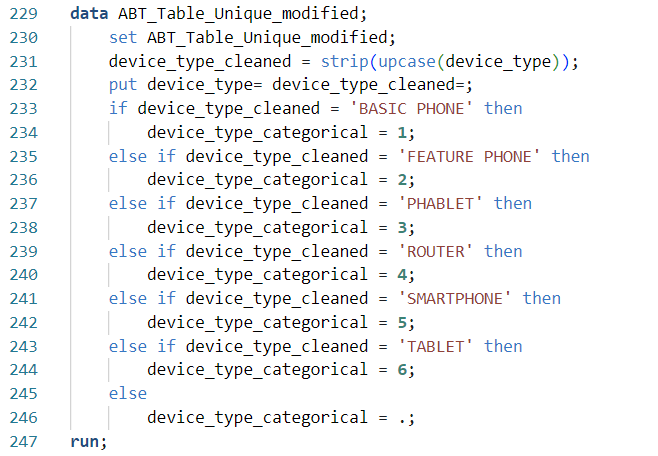
\includegraphics[width=0.5\textwidth]{capture_sas_3.png}
        \caption{Exemple de transformation des variables catégorielles}
        \label{fig:categorical_example}
    \end{figure}

    \item \textbf{Variables quantitatives:} En ce qui concerne les variables quantitatives, telles que les minutes d'appel (\textbf{mou}) ou les SMS envoyés (\textbf{number\_of\_sms}), on a procédé à une agrégation des sous-catégories pour obtenir des variables globales. Par exemple, la variable \textbf{mou\_m1} regroupe les minutes d'appels \textbf{onnet}, \textbf{offnet}, et \textbf{internationales}. Cela permet de simplifier l'analyse tout en conservant la pertinence des données.

    \begin{figure}[H]
        \centering
        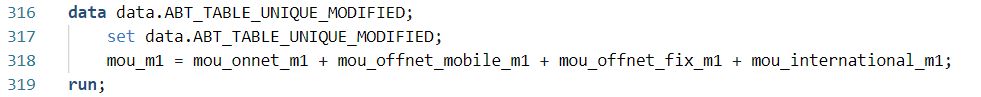
\includegraphics[width=0.7\textwidth]{capture_sas_4.png}
        \caption{Exemple d'agrégation des variables quantitatives}
        \label{fig:quantitative_example}
    \end{figure}

    \item \textbf{Variable cible binaire:} On a également créé une nouvelle variable binaire, \textbf{osat\_binary}, qui représente la satisfaction des clients de manière simplifiée. Les valeurs 1 et 2 de la variable \textbf{OSAT} sont considérées comme insatisfaction (codées par 1), tandis que les valeurs 3, 4 et 5 sont regroupées sous la catégorie satisfaction (codées par 0). Cette transformation facilite l'application de modèles de classification binaire.

\end{itemize}

Ces transformations garantissent que les données, tant qualitatives que quantitatives, sont consolidées et normalisées pour assurer une analyse cohérente et robuste.


\noindent \textbf{\checkmark Fusion des tables et agrégation:} on a fusionner les tables \textbf{Resp\_Network\_Fev} et \textbf{monthly\_aggregation} pour obtenir une table finale. La variable \textbf{OSAT} est extraite de \textbf{Resp\_Network\_Fev} et intégrée dans la table finale. Celle-ci contient les comportements clients sur plusieurs mois ainsi que leur score de satisfaction.
La table finale agrégée comprend \textbf{25 colonnes} et \textbf{985 lignes}. Elle regroupe les informations prêtes pour l'analyse. Voici les colonnes principales :

\begin{longtable}{|p{7cm}|p{9cm}|}
    \hline
    \textbf{Nom de la variable} & \textbf{Description} \\ \hline
    \textbf{msisdn} & Identifiant unique du client \\ \hline
    \textbf{OSAT} & Score de satisfaction global \\ \hline
    \textbf{subscriber\_activation\_date\_only} & Date d'activation du client \\ \hline
    \textbf{Indicator\_vas} & Utilisation des services à valeur ajoutée \\ \hline
    \textbf{monthly\_rech\_subscriber\_seg} & Montant moyen des recharges mensuelles \\ \hline
    \textbf{monthly\_arpu\_subscriber\_seg} & Revenu moyen par utilisateur \\ \hline
    \textbf{Number\_of\_reactivation} & Nombre de réactivations \\ \hline
    \textbf{Flag\_4g\_binary} & Utilisation de la 4G (binaire) \\ \hline
    \textbf{device\_type} & Type d'appareil \\ \hline
    \textbf{flag\_smartphone} & Indique un smartphone \\ \hline
    \textbf{recharge\_moyenne} & Montant moyen des recharges \\ \hline
    \textbf{Arpu\_moyenne} & Revenu moyen \\ \hline
    \textbf{data\_volume\_moyenne} & Volume moyen de données \\ \hline
    \textbf{mou\_moyenne} & Moyenne des minutes d'appels \\ \hline
    \textbf{nbre\_recharges\_moyenne} & Nombre moyen de recharges \\ \hline
    \textbf{nbre\_sms\_moyenne} & Nombre moyen de SMS \\ \hline
    \textbf{voice\_amount\_moyenne} & Montant moyen des appels vocaux \\ \hline
    \textbf{data\_amount\_moyenne} & Montant moyen des données utilisées \\ \hline
    \textbf{voice\_volume\_moyenne} & Volume moyen des appels \\ \hline
\caption{Colonnes principales de la table finale.}
\label{table:variables_final}
\end{longtable}
\textbf{\checkmark Gestion des valeurs manquantes:}
\begin{enumerate}
    \item \textbf{Imputation pour OSAT:} Certaines lignes de la table \textbf{Resp\_Network\_Fev} contenaient des valeurs manquantes dans la colonne \textbf{OSAT}. On a imputé ces valeurs en utilisant la moyenne des réponses aux questions \textbf{q3} à \textbf{q18}. Le code complet pour cette imputation est disponible dans l'annexe (voir figure \ref{imputation_code}).

    \item \textbf{Imputation pour subscriber\_activation\_date\_only:} Un total de \textbf{114 valeurs manquantes} a été détecté dans cette colonne. Pour y remédier, on a utilisé \textbf{KNNImputer} et l'imputation par la médiane via \textbf{Jupyter Notebook}. 

    Avant l'imputation, les dates ont été converties en jours depuis une date de référence (\textbf{01/01/1970}), créant une variable \textbf{activation\_days}. La colonne d'origine a ensuite été supprimée.

    \textbf{Imputation KNN:} On a appliqué \textbf{KNNImputer} avec 5 voisins pour estimer les valeurs manquantes, en se basant sur la similarité avec les autres colonnes. Pour le code complet utilisé dans cette méthode, référez-vous à la figure \ref{fig:knn_code} dans l'annexe.

    \textbf{Imputation par la médiane:} En complément, on a testé l'imputation par la médiane pour comparer avec KNN et identifier la méthode la plus fiable.

\end{enumerate}

\subsection{Normalisation des données}

La normalisation est essentielle pour rendre les variables comparables et améliorer les performances des algorithmes d'apprentissage.

\textbf{\checkmark Gestion des valeurs aberrantes:}  
On a identifié et remplacé les valeurs aberrantes des variables quantitatives (montants de recharge, volume de données, SMS, minutes d'appels) en utilisant les quartiles (\textbf{Q1}, \textbf{Q3}) et l'intervalle interquartile (\textbf{IQR}). Les valeurs en dehors de l'intervalle (\textbf{Q1 - 1.5 * IQR} à \textbf{Q3 + 1.5 * IQR}) ont été remplacées par la médiane pour éviter les biais. Le code utilisé pour cette étape est disponible dans l'annexe (voir figure \ref{fig:aberrant_values_annex}).

\textbf{\checkmark Normalisation Box-Cox:}  
Après avoir géré les valeurs aberrantes, différentes méthodes de normalisation (\textbf{min-max}, \textbf{sqrt}, \textbf{log}) ont été testées sans succès. On a donc appliqué la transformation \textbf{Box-Cox}, particulièrement efficace pour les données asymétriques. L'algorithme a optimisé la valeur de \(\lambda\) à l'aide de la courbe de log-vraisemblance. La transformation a été appliquée à la variable \textbf{Recharge\_moyenne}, créant la nouvelle variable normalisée \textbf{new\_recharge\_moyenne}. Le code détaillé est présenté dans l'annexe (voir figure \ref{fig:boxcox_transformation_annex}).

Après la transformation et la gestion des valeurs aberrantes, on a vérifié la distribution des données normalisées via les histogrammes. La normalité a aussi été testée avec Shapiro-Wilk, mais les résultats ne sont pas disponibles en raison d'un problème sur la plateforme SAS en fin de stage. Cependant, les premiers résultats montrent que la normalité n'est pas totalement vérifiée, bien que les données de cette table soient presque normales. La table a été exportée en format Excel pour l'analyse et la modélisation sur Jupyter, offrant plus de flexibilité et rapidité.

\subsection{Utilisation de plusieurs tables}

\textbf{\checkmark Application sur plusieurs jeux de données:}  
Le processus de prétraitement a été appliqué à plusieurs jeux de données pour garantir la pertinence et la continuité temporelle. On a traité les tables \textbf{Resp\_Network\_Fev}, \textbf{network\_may} et \textbf{retail\_juin}, couvrant les périodes de février à juin. Chaque table contient des colonnes similaires et a été soumise au même processus de nettoyage et de transformation.

\noindent \textbf{\checkmark Comparaison des échantillons:}  
La table \textbf{network\_may} contient 375 lignes, un échantillon relativement réduit. Pour obtenir des résultats plus représentatifs, on a également utilisé \textbf{retail\_juin}, qui compte 2554 lignes. Cela permet d'analyser les variations temporelles et d'assurer la robustesse des résultats.

\noindent \textbf{\checkmark Pourquoi trois datasets ?}  
L'utilisation de ces trois tables permet de comparer les performances des modèles sur différentes périodes, d'analyser les tendances comportementales, et d'évaluer la persistance des schémas.

\noindent \textbf{Détails sur les trois tables:}  
\begin{itemize}
    \item \textbf{Resp\_Network\_Fev}: 985 lignes, 114 valeurs manquantes pour \textbf{activation\_days}.
    \item \textbf{network\_may}: 375 lignes, 44 valeurs manquantes.
    \item \textbf{retail\_juin}: 2554 lignes, 281 valeurs manquantes.
\end{itemize}

\noindent \textbf{\checkmark Difficultés de normalisation:}  
Malgré les efforts, la normalisation des données dans \textbf{network\_may} et \textbf{retail\_juin} n'a pas réussi pour certaines variables, même avec les méthodes \textbf{min-max}, \textbf{sqrt}, \textbf{log}, et \textbf{Box-Cox}. Cela sera pris en compte lors de l'analyse des résultats.

\noindent \textbf{\checkmark Travail avec les trois tables:}  
Les trois jeux de données seront utilisés pour:
\begin{itemize}
    \item Comparer les performances des modèles,
    \item Évaluer la robustesse des résultats sur plusieurs périodes,
    \item Identifier les différences comportementales entre les clients.
\end{itemize}

Ces trois jeux de données, bien que présentant des défis de normalisation, offrent une base solide pour l'analyse et la modélisation prédictive.

\section{Analyse des données}
L'analyse des données comprend à la fois une exploration descriptive des variables et une analyse inférentielle pour extraire des conclusions significatives.

\subsection{Analyse descriptive}

L'analyse descriptive a été réalisée sur la variable \textbf{recharge}, en examinant son comportement par rapport à la variable \textbf{OSAT}, à la fois en version multiclasse et binaire.
\subsubsection{Analyse des variables quantitatives}

\subsubsection*{Analyse pour la variable Recharge}
Les statistiques descriptives pour la variable \textbf{recharge} selon les classes \textbf{OSAT} multiclasse sont présentées à travers la distribution de la variable par classe dans la figure \ref{fig:analyse_descriptive_2}.

\begin{figure}[H]
    \centering
    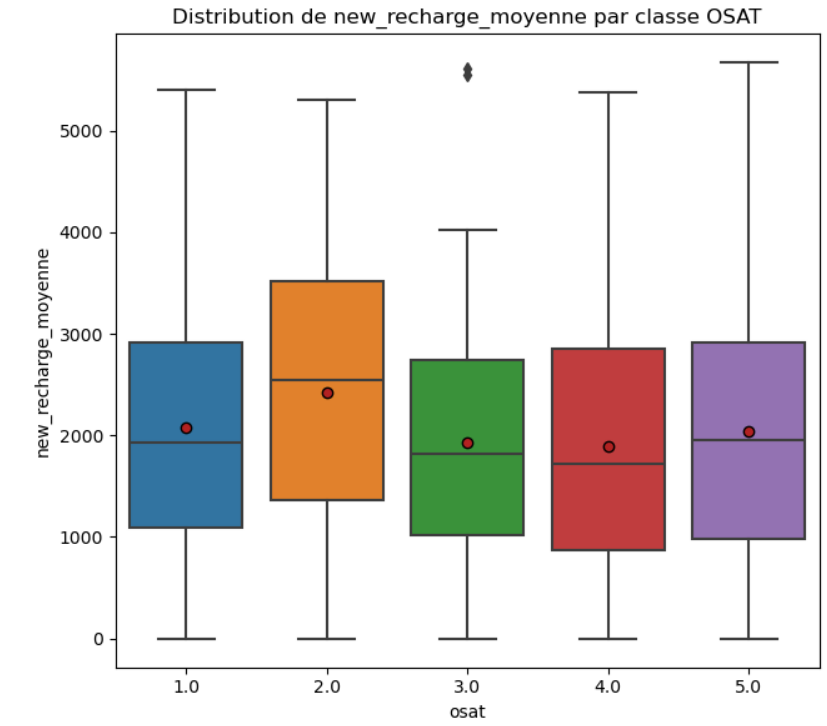
\includegraphics[width=0.7\linewidth]{analyse_descriptive_2.png}
    \caption{Distribution de la variable \textbf{recharge} par classe \textbf{OSAT} multiclasse.}
    \label{fig:analyse_descriptive_2}
\end{figure}

Les moyennes de \textbf{recharge} montrent une légère variation entre les classes \textbf{OSAT} multiclasse. Les classes 2 et 5 présentent des médianes plus élevées, tandis que la classe 1 a une médiane légèrement inférieure. Comme le montre la figure \ref{fig:analyse_descriptive_2}, la distribution de \textbf{recharge} est relativement similaire entre les classes, bien que les médianes des classes 2 et 5 soient plus élevées.

Passons maintenant à la comparaison avec \textbf{OSAT} binaire.

Les statistiques descriptives pour la variable \textbf{recharge} selon les classes \textbf{OSAT} binaire sont présentées dans le tableau ci-dessous.

\begin{table}[H]
    \centering
    \begin{tabular}{p{2cm}ccccccccc} % 9 columns
        \toprule
        Classe OSAT binaire & Nombre & Moyenne & Ecart-Type & Min & Q1 & Médiane & Q3 & Max \\
        \midrule
        0 & 334 & 2158.66 & 1323.81 & -1.33 & 1161.87 & 2041.87 & 3107.40 & 5405.60 \\
        1 & 651 & 1966.57 & 1310.51 & -1.33 & 907.64 & 1835.88 & 2881.57 & 5670.04 \\
        \bottomrule
    \end{tabular}
    \caption{Statistiques descriptives de la variable \textbf{recharge} selon la classe \textbf{OSAT} binaire.}
\end{table}

Dans la version binaire, la moyenne de \textbf{recharge} pour la classe 0 est légèrement plus élevée que celle de la classe 1, mais la variabilité est similaire entre les deux groupes, comme le montre l'écart-type.

\subsubsection*{Comparaison entre les OSAT multiclasse et OSAT binaire pour la variable recharge} 
Bien que la version multiclasse de \textbf{OSAT} offre une segmentation plus détaillée, les différences entre les classes pour la variable \textbf{recharge} ne sont pas assez marquantes pour justifier une complexité supplémentaire. Les moyennes dans la version binaire sont similaires entre les classes 0 et 1, avec une variabilité légère qui n'altère pas l'interprétation globale. Par conséquent, pour simplifier l'analyse tout en assurant une cohérence des résultats, la version binaire est privilégiée.

\subsubsection*{Analyse pour les variables quantitatives}

L'analyse des variables quantitatives selon OSAT multiclasse et OSAT binaire révèle des tendances intéressantes. Voici les points principaux :

\noindent \textbf{ARPU:} \\
\textbf{OSAT multiclasse}: L'ARPU moyen varie légèrement entre les classes (255 à 301). Les classes 2 et 5 présentent les valeurs moyennes les plus élevées, reflétant une consommation plus importante de ces groupes. \\
\textbf{OSAT binaire}: La différence entre les classes 0 et 1 est faible (278 vs 275), avec une variabilité similaire entre les deux groupes.

\vspace{0.2cm}

\noindent \textbf{Volume d'appels (voice\_volume):} \\
\textbf{OSAT multiclasse}: Les moyennes sont stables entre les classes (38 à 43), avec une légère augmentation pour les classes 4 et 5. \\
\textbf{OSAT binaire}: Différence marginale entre les classes 0 et 1 (41,27 vs 42,28), avec une distribution homogène.

\vspace{0.2cm}

\noindent \textbf{Nombre d'appels (voice\_amount):} \\
\textbf{OSAT multiclasse}: Les moyennes varient peu entre les classes, la classe 5 étant légèrement plus élevée. \\
\textbf{OSAT binaire}: Différence minime entre les classes 0 et 1 (28,23 vs 28,65).

\vspace{0.2cm}

\noindent \textbf{Volume de données (data\_volume):} \\
\textbf{OSAT multiclasse}: La classe 2 présente une consommation de données plus élevée (2,33), tandis que les autres classes sont plus homogènes. \\
\textbf{OSAT binaire}: La classe 0 consomme légèrement plus de données que la classe 1 (2,21 vs 1,96).

\vspace{0.2cm}

\noindent \textbf{Nombre de transactions de données (data\_amount):} \\
\textbf{OSAT multiclasse}: Légère différence entre les classes, avec un pic pour la classe 5 (202). \\
\textbf{OSAT binaire}: La classe 0 réalise plus de transactions que la classe 1 (205 vs 195), mais la différence reste minime.

\vspace{0.2cm}

\noindent \textbf{Activation Days:} \\
\textbf{OSAT multiclasse}: La moyenne des jours d'activation varie légèrement entre les classes, avec les valeurs les plus élevées pour les classes 3 et 4, correspondant à environ 47,1 ans et 46,3 ans respectivement. \\
\textbf{OSAT binaire}: La différence entre les classes 0 et 1 est minime, avec des durées moyennes d'activation d'environ 46,6 ans (classe 0) et 46,3 ans (classe 1), ce qui montre une stabilité dans la durée d'activation entre ces deux groupes.

\vspace{0.2cm}

\noindent \textbf{Minutes of Usage (MOU):} \\
\textbf{OSAT multiclasse}: Les moyennes des minutes d'utilisation varient entre 32 et 38 minutes, avec une légère augmentation pour les classes 4 et 5. \\
\textbf{OSAT binaire}: Les différences entre les classes 0 et 1 sont faibles (35,52 vs 36,82 minutes), ce qui indique une utilisation similaire des services vocaux dans les deux groupes.

\vspace{0.2cm}

\noindent \textbf{Nombre de SMS:} \\
\textbf{OSAT multiclasse}: Le nombre moyen de SMS varie entre 6,71 et 7,86 selon les classes, avec une légère augmentation pour la classe 2, ce qui suggère une utilisation plus importante de cette classe. \\
\textbf{OSAT binaire}: La différence entre les classes 0 et 1 est faible (7,37 vs 6,97), indiquant une consommation de SMS relativement comparable entre ces deux classes.

\vspace{0.2cm}

\subsubsection*{Comparaison générale entre OSAT multiclasse et OSAT binaire} 
Dans l'ensemble, la version multiclasse d'OSAT permet une segmentation plus fine, mais les différences observées entre les classes pour l'ensemble des variables quantitatives sont généralement minimes. La version binaire offre une simplification sans perte significative d'information, ce qui la rend plus appropriée pour les prochaines analyses en réduisant la complexité tout en maintenant une interprétation claire.

\subsubsection{Analyse des variables qualitative}
\subsubsection*{Analyse pour la variable qualitative \textbf{monthly\_rech\_subscriber\_seg}}

L'analyse de la variable \textbf{monthly\_rech\_subscriber\_seg} selon les classes \textbf{OSAT} multiclasse est illustrée par la figure ci-dessous.

\begin{figure}[H]
    \centering
    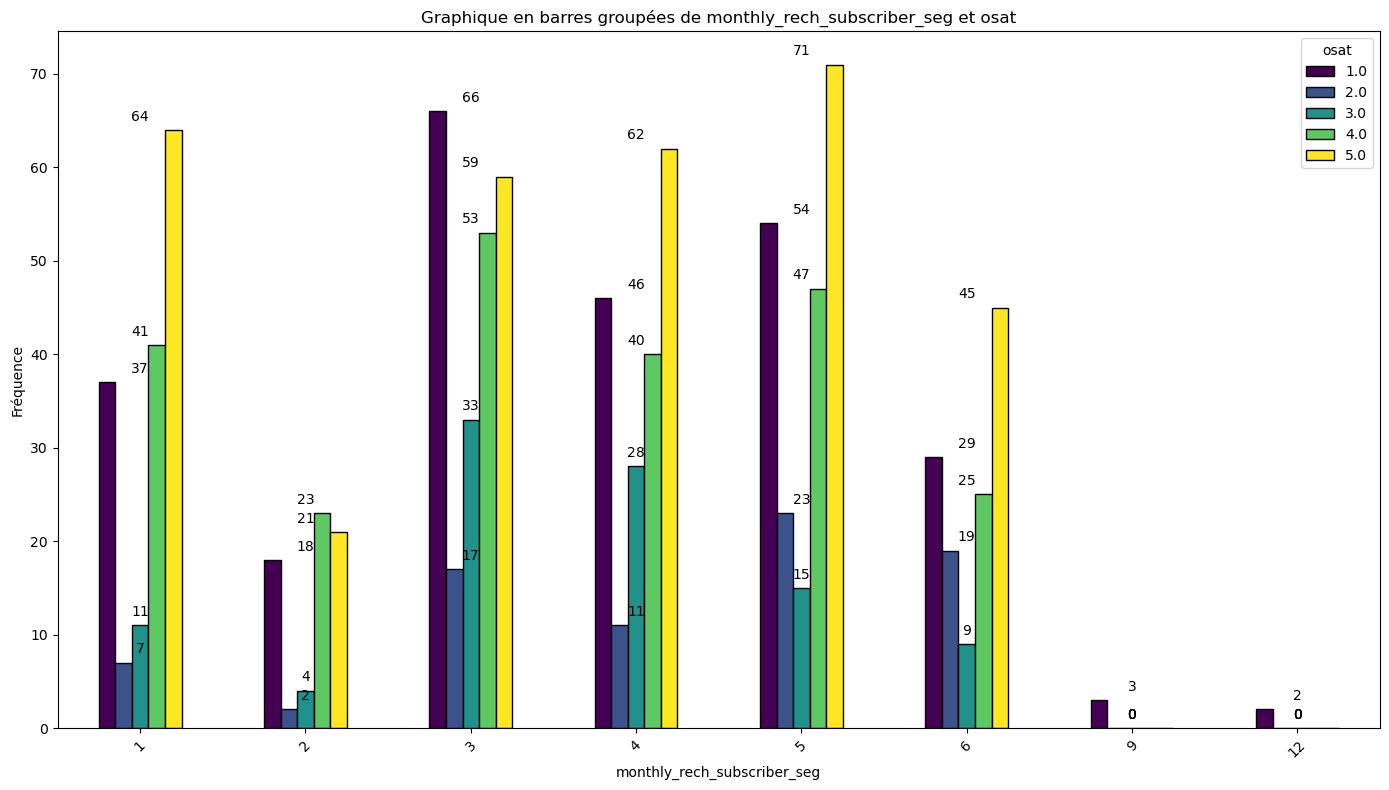
\includegraphics[width=0.7\linewidth]{barre_monthl_rech.png}
    \caption{Distribution de la variable \textbf{monthly\_rech\_subscriber\_seg} par classe \textbf{OSAT} multiclasse.}
    \label{fig:barre_monthl_rech}
\end{figure}

Comme le montre la figure \ref{fig:barre_monthl_rech}, les classes 1 et 5 sont les plus représentées dans les segments de recharge mensuelle, notamment dans les segments 1 et 6, avec une fréquence plus élevée. Les autres classes, telles que les classes 2, 3 et 4, sont moins représentées dans ces segments, ce qui indique une disparité dans les comportements de recharge des utilisateurs selon leur classe d'OSAT.

Passons maintenant à la comparaison avec \textbf{OSAT} binaire.

\begin{figure}[H]
    \centering
    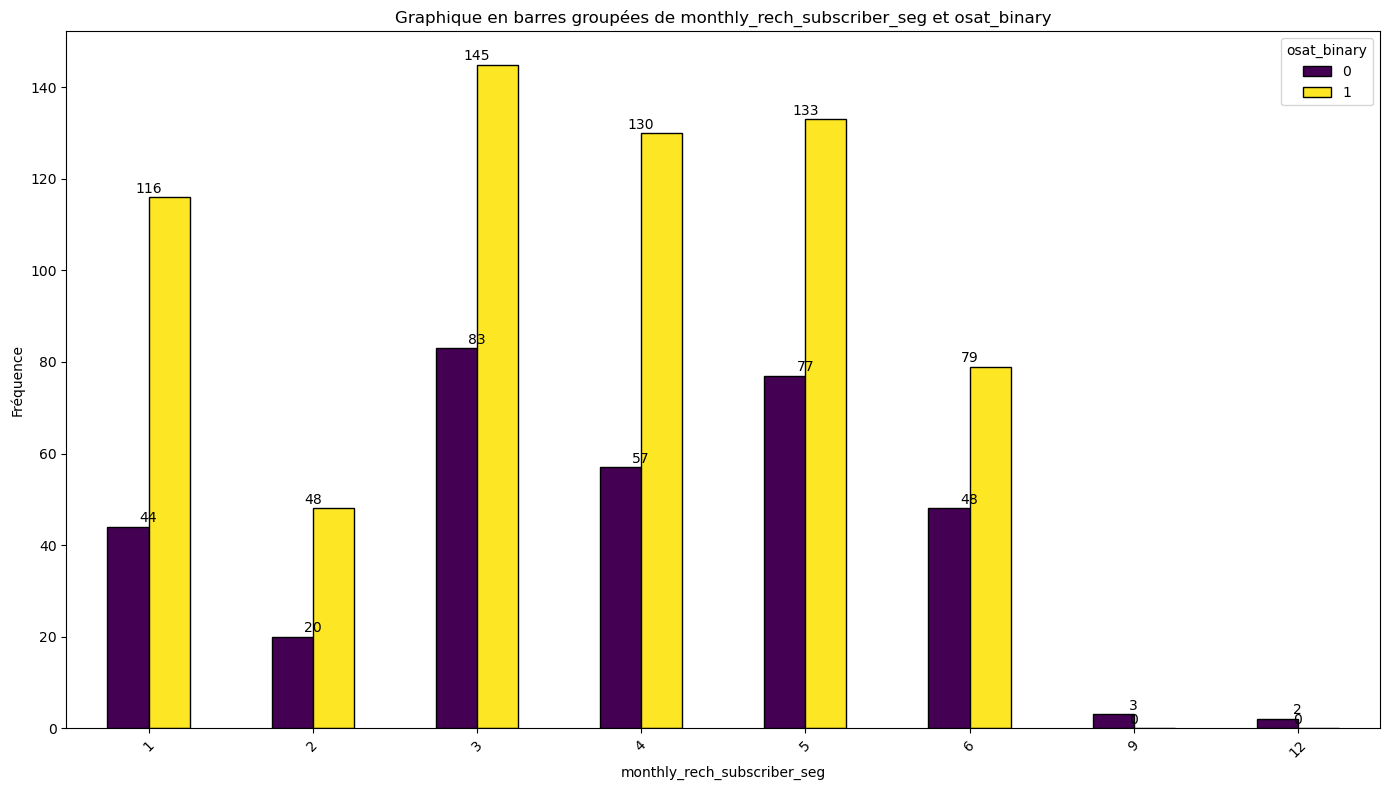
\includegraphics[width=0.7\linewidth]{barre_monthl_rech_binary.png}
    \caption{Distribution de la variable \textbf{monthly\_rech\_subscriber\_seg} par classe \textbf{OSAT} binaire.}
    \label{fig:barre_monthl_rech_binary}
\end{figure}

Dans la version binaire, comme le montre la figure \ref{fig:barre_monthl_rech_binary}, les utilisateurs satisfaits (classe 1) sont largement dominants dans tous les segments de recharge mensuelle, particulièrement dans les segments 3 et 5. À l'inverse, les utilisateurs insatisfaits (classe 0) sont moins présents, ce qui reflète un comportement de recharge moins intense pour cette classe.

\subsubsection*{Comparaison entre les OSAT multiclasse et OSAT binaire pour la variable \textbf{monthly\_rech\_subscriber\_seg}} 
Bien que la version multiclasse de \textbf{OSAT} offre une segmentation plus fine, les tendances principales se retrouvent également dans la version binaire. La classe 1 (satisfaits) montre une fréquence plus élevée dans les segments de recharge les plus importants (3 et 5). Par conséquent, la version binaire est privilégiée pour les analyses ultérieures afin de simplifier les interprétations sans perdre d'informations significatives.

\subsubsection*{Analyse récapitulative pour les variables qualitatives}

Les variables qualitatives ont été analysées en fonction des segments \textit{OSAT multiclasse} et \textit{OSAT binaire}. Voici un aperçu des résultats pour chaque variable.

\begin{table}[H]
    \centering
    \begin{tabular}{|p{3.5cm}|p{3.5cm}|p{3.5cm}|p{3.5cm}|} 
    \hline
    \textbf{Variable} & \textbf{OSAT multiclasse} & \textbf{OSAT binaire} & \textbf{Observations générales} \\ 
    \hline
    \textit{Device Type} & 
    La classe 3 présente des valeurs élevées & 
    Les valeurs sont concentrées dans la classe 1 & 
    Segment 3 reste important dans les deux OSAT \\ 
    \hline
    \textit{Monthly ARPU Subscriber Seg} & 
    La classe 12 a des valeurs très élevées & 
    Segment 12 montre une prédominance de classe 1 & 
    Segment 12 est dominant dans les deux OSAT \\ 
    \hline
    \textit{Flag 4G Binary} & 
    Classe 1 contient la majorité des utilisateurs 4G & 
    La classe 1 reste dominante dans le segment 4G & 
    Une forte majorité est 4G dans les deux OSAT \\ 
    \hline
    \textit{Flag Smartphone} & 
    Les classes 1 et 5 montrent une grande utilisation de smartphones & 
    La majorité des utilisateurs sont dans la classe 1 & 
    Utilisation généralisée de smartphones dans les deux OSAT \\ 
    \hline
    \textit{Number of Reactivation} & 
    Classe 1 a des réactivations élevées & 
    Les réactivations sont dominées par la classe 0 & 
    Répartition similaire dans les deux OSAT \\ 
    \hline
    \end{tabular}
    \caption{Résumé des variables qualitatives entre \textit{OSAT multiclasse} et \textit{OSAT binaire}.}
\end{table}

\subsubsection*{Comparaison générale entre OSAT multiclasse et OSAT binaire pour les variables qualitatives}
La version multiclasse d'OSAT offre une segmentation plus détaillée des variables qualitatives, mais les différences entre les classes restent souvent subtiles. La version binaire simplifie l'analyse sans perte majeure d'information, facilitant ainsi l'interprétation tout en réduisant la complexité. Pour les prochaines analyses, OSAT binaire est privilégiée en raison de son efficacité et de sa clarté.

\subsubsection{Comparaison globale entre OSAT multiclasse et OSAT binaire}
L'analyse des variables quantitatives et qualitatives montre que, bien que la version multiclasse d'OSAT permette une segmentation plus fine, les différences observées entre les classes sont généralement minimes. La version binaire d'OSAT simplifie l'interprétation sans perte significative d'information. Cette simplification réduit la complexité des analyses tout en maintenant une clarté et une cohérence suffisantes dans les résultats. Par conséquent, l'utilisation d'OSAT binaire est privilégiée pour les prochaines étapes, car elle permet une analyse plus efficace et facile à interpréter.


\subsection{Analyse inférentielle}

L'objectif de l'analyse inférentielle est de comprendre les relations entre la variable cible (\textbf{OSAT}) et les différentes \textbf{features} explicatives, qu'elles soient quantitatives ou qualitatives. Dans cette section, nous explorons la corrélation entre les variables qualitatives et quantitatives, ainsi que la corrélation entre variables qualitatives elles-mêmes.
on a d'abord examiné la corrélation entre la variable cible (\textbf{OSAT}) et les différentes \textbf{features} quantitatives. L'analyse de corrélation est illustrée par une matrice de corrélation, dans laquelle on a utilisé le coefficient de corrélation de Pearson pour évaluer la relation linéaire entre les variables.
\begin{figure}[H]
    \centering
    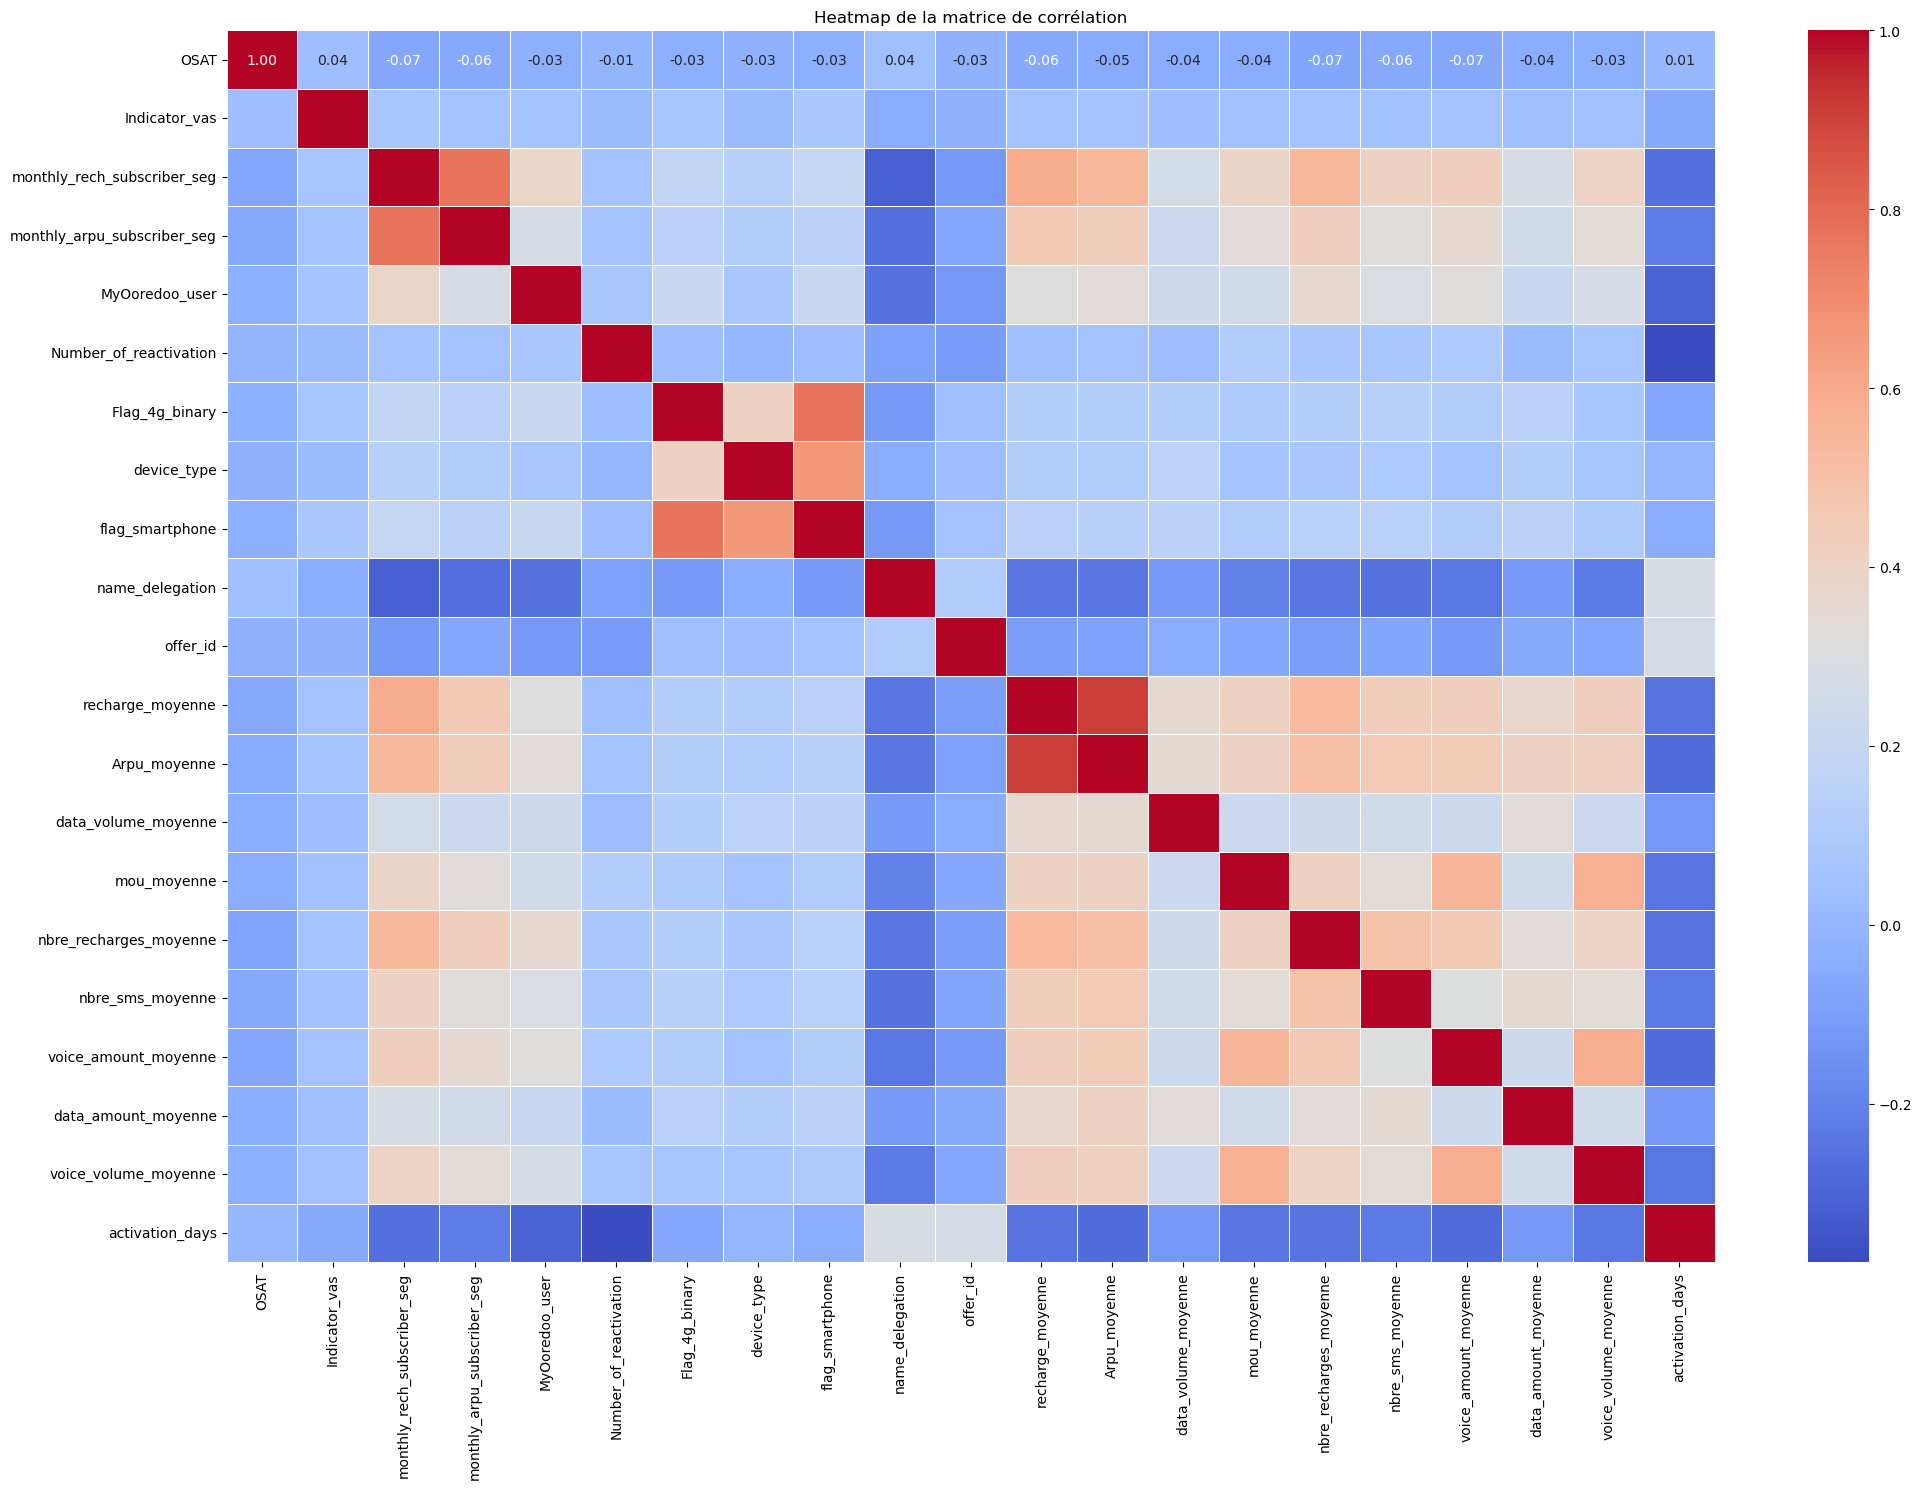
\includegraphics[width=0.7\linewidth]{Correlation_Retail.png}
    \caption{Heatmap de la matrice de corrélation globale pour la table de Juin.}
    \label{fig:correlation_matrix}
\end{figure}

\subsubsection{Corrélation entre la variable cible et les variables explicatives}
\subsubsection*{Corrélation entre les variables qualitatives et la variable cible}

Pour évaluer la relation entre des variables qualitatives comme \textbf{device\_type} et \textbf{osat}, plusieurs indicateurs statistiques ont été utilisés, notamment \textbf{Cramér's V} et le \textbf{test du Chi-Carré}, afin de mesurer et évaluer la force de leur association.

\textbf{1. Indice de Cramér’s V:} Cet indice mesure la force de l'association entre deux variables qualitatives. L'indice de Cramér’s V varie entre 0 et 1, où une valeur proche de 0 indique une faible association et une valeur proche de 1 indique une association forte.

\textit{Le code utilisé pour calculer cet indice est présenté dans l'annexe, voir Figure \ref{00}.}

\textbf{\checkmark Exemple de résultat:} Pour la relation entre \textbf{device\_type} et \textbf{osat}, un Cramér's V de \textbf{0.0297} a été obtenu, ce qui indique une association faible.

    
\textbf{2. Test du Chi-Carré:} Ce test permet de vérifier s'il existe une association statistiquement significative entre deux variables qualitatives. Si la p-value est inférieure à 0.05, cela indique une association significative.

\textit{Le code utilisé pour effectuer le test du Chi-Carré est présenté dans l'annexe, voir Figure \ref{222}.}

Pour la relation entre \textbf{device\_type} et \textbf{osat\_binary} (binarisation d'OSAT), une p-value de \textbf{0.7528} a été obtenue, indiquant qu'il n'y a pas d'association significative.

\textbf{\checkmark Exemple de tableau de contingence:}

\begin{figure}[H]
    \centering
    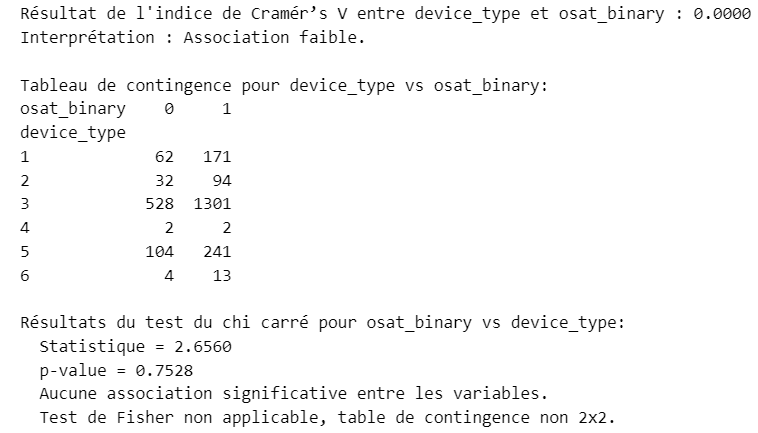
\includegraphics[width=0.6\linewidth]{capture_sas_39.png}
    \caption{Tableau de contingence pour \textbf{device\_type} et \textbf{osat\_binary}.}
\end{figure}

Le test du Chi-Carré confirme qu'il n'y a pas d'association significative entre \textbf{device\_type} et \textbf{osat\_binary} (p-value = 0.7528). Le test de Fisher n'était pas applicable, car le tableau de contingence n'était pas de dimension 2x2.

Cette méthodologie a été appliquée pour toutes les autres variables qualitatives.

\textbf{\(\rightarrow\)} \textbf{Variables avec faible association:} Certaines variables montrent une faible association avec la satisfaction (\textbf{OSAT}), notamment \textbf{monthly\_arpu\_subscriber\_seg}, \textbf{monthly\_rech\_subscriber\_seg}, \textbf{flag\_smartphone}, et \textbf{Number\_of\_reactivation}. Les indices de \textbf{Cramér's V} sont inférieurs à 0.1 et les \textbf{p-values} du \textbf{Chi-Carré} dépassent 0.05, indiquant une faible ou aucune association statistiquement significative.


\textbf{\(\rightarrow\)} \textbf{Variables sans association significative:} Les variables \textbf{Flag\_4g\_binary} et \textbf{flag\_smartphone} n’ont montré aucune association avec \textbf{osat\_binary}. Les \textbf{p-values} sont supérieures à 0.05, confirmant l'absence de relation statistiquement significative.

\textbf{\(\rightarrow\)} \textbf{Variable avec une association significative:} La variable \textbf{monthly\_rech\_subscriber\_seg} montre une association significative avec une \textbf{p-value} de \textbf{0.0211}, suggérant un impact potentiel sur la satisfaction (\textbf{osat\_binary}).\par

\textbf{3. Analyse de l'association par la Lambda de Goodman et Kruskal:} Pour approfondir l'analyse des relations entre les variables qualitatives et \textbf{osat\_binary}, on a calculé la \textbf{Lambda de Goodman et Kruskal}, qui évalue la réduction d'erreur dans la prédiction d'une variable en fonction d'une autre.

\textit{Le code utilisé pour calculer la Lambda de Goodman et Kruskal est présenté dans l'annexe, voir Figure \ref{555}.}

\textbf{\checkmark Exemple de résultat:} Pour la variable \textbf{Flag\_4g\_binary}, une Lambda de \textbf{0.42} a été obtenue, indiquant que la connaissance de cette variable permet une réduction d'erreur de \textbf{42\%} dans la prédiction de \textbf{osat\_binary}.

\textit{Le résultat de la Lambda de Goodman et Kruskal est présenté dans l'annexe, voir Figure \ref{AnB1}.}


\textbf{\checkmark Résultats pour les autres variables:} Les résultats montrent que \textbf{device\_type} a une lambda de 0.15, indiquant une faible réduction d'erreur, tandis que \textbf{flag\_smartphone} et \textbf{Number\_of\_reactivation} affichent des lambdas de 0.60 et 0.84 respectivement, signalant une réduction d'erreur plus significative. En revanche, \textbf{monthly\_arpu\_subscriber\_seg} et \textbf{monthly\_rech\_subscriber\_seg} n'ont aucune réduction d'erreur avec des lambdas nulles.

Cela montre que certaines variables, comme \textbf{flag\_smartphone} et \textbf{Number\_of\_reactivation}, influencent la satisfaction (\textbf{osat\_binary}), tandis que d'autres, comme \textbf{monthly\_arpu\_subscriber\_seg}, n'apportent aucune valeur prédictive.

\subsubsection*{Corrélation entre les variables quantitatives et la variable cible}

Pour évaluer la relation entre les variables quantitatives et la variable cible \textbf{osat\_binary}, on a utilisé l'indicateur de \textbf{l'Eta carré}. Cet indicateur permet de mesurer l'effet de la variable explicative sur la variable cible. Le calcul de l'Eta carré a été effectué pour \textbf{osat\_binary}.

\textit{Le code utilisé pour calculer l'Eta carré est présenté en annexe, voir Figure \ref{26203}.}

Ensuite, pour déterminer le test statistique à utiliser, on a vérifié la normalité et l'homogénéité des variances avec les tests de \textbf{Shapiro-Wilk} et \textbf{Levene}. Si les conditions étaient remplies, on a utilisé le \textbf{test t de Student}. Sinon, le \textbf{test de Mann-Whitney} a été appliqué.

\textit{Le code de ces tests est disponible en annexe, voir Figure \ref{168}.}

\textbf{Résultats pour la variable Recharge:}

Pour la variable quantitative \textbf{recharge}, l'ensemble des tests a été appliqué afin d'évaluer son association avec \textbf{OSAT}. Voici les résultats obtenus à chaque étape.

\textbf{\checkmark Résultat de l'Eta carré:} L'indicateur de \textbf{l'Eta carré} montre un effet très faible pour \textbf{OSAT}, avec une valeur de \textbf{0.0064}. 

\textit{Résultat de l'Eta carré pour osat\_binary est disponible en annexe, voir Figure \ref{AnB3}.}


L'interprétation de ce résultat indique que l'effet de la variable explicative sur la satisfaction (\textbf{OSAT}) est très faible, suggérant une influence limitée.

\textbf{\checkmark Test pour \textbf{osat\_binary}:} Les tests de \textbf{Shapiro-Wilk} montrent que les données ne suivent pas une distribution normale pour les deux groupes (statistiques de \textbf{0.7522} pour le groupe 0 et \textbf{0.6954} pour le groupe 1, avec des p-values inférieures à 0.05). De plus, le test de \textbf{Levene} indique que les variances ne sont pas homogènes (\textbf{p-value = 0.0273}). Par conséquent, les conditions pour appliquer un test paramétrique ne sont pas respectées. Nous avons donc appliqué le \textbf{test de Mann-Whitney}, qui révèle des différences significatives entre les deux groupes (\textbf{p-value = 0.0003}). 


\textit{Les résultats du test de normalité et de variances et du test de Mann-Whitney sont disponibles en annexe, voir Figure \ref{AnB4} et \ref{AnB5}.}



Les résultats du test de Mann-Whitney montrent une différence significative entre les distributions de la variable \textbf{recharge\_moyenne} pour les deux groupes de \textbf{osat\_binary} (\textbf{p-value = 0.0003}), indiquant que les valeurs de \textbf{recharge\_moyenne} diffèrent significativement selon les niveaux de \textbf{osat\_binary}.

Pour \textbf{osat multiclasse}, les tests ont montré des résultats similaires avec des différences significatives entre les groupes (p-value = 0.0003).

\textbf{Conclusion des tests:} Les tests de normalité (\textbf{Shapiro-Wilk}) et d'homogénéité des variances (\textbf{Levene}) n'ont pas été vérifiés pour les variables quantitatives étudiées. Par exemple, pour \textbf{Arpu}, le test de Shapiro-Wilk a donné des p-values de \textbf{0.0000}, indiquant une distribution non normale. Bien que certaines variables, comme \textbf{Arpu}, aient montré des variances homogènes (p = \textbf{0.0801}), les conditions d'application des tests paramétriques n'ont globalement pas été respectées.

En conséquence, tous les tests utilisés sont non paramétriques : le \textbf{Mann-Whitney} pour \textbf{osat\_binary} et le \textbf{Kruskal-Wallis} pour \textbf{OSAT}. Lorsque des différences significatives ont été détectées avec Kruskal-Wallis, des comparaisons post-hoc ont été effectuées avec le test de \textbf{Dunn}. Le tableau ci-dessous résume les résultats :

\begin{longtable}{|l|c|c|c|p{3cm}|}
\hline
\textbf{Variable} & \textbf{Eta carré} & \textbf{Test U (osat\_binary)} & \textbf{Kruskal-Wallis (osat)} &  \textbf{Interprétation finale} \\ 
\hline
\textbf{Arpu} & 0.0057 & p = 0.0005 & p = 0.0011 & Différences significatives \\ 
\hline
\textbf{Voice volume} & 0.0047 & p = 0.0008 & p = 0.0001  & Différences significatives \\ 
\hline
\textbf{Voice amount} & 0.0078 & p = 0.0001 & p = 0.0001  & Différences significatives \\ 
\hline
\textbf{Data volume} & 0.0029 & p = 0.1979 & p = 0.2741  & Pas de différences significatives \\ 
\hline
\textbf{Mou} & 0.0042 & p = 0.0003 & p = 0.0002  & Différences significatives \\ 
\hline
\textbf{Nbre of SMS} & 0.0058 & p = 0.0038 & p = 0.0054 & Différences significatives \\ 
\hline
\textbf{Activation days} & - & p = 0.8498 & p = 0.6350  & Pas de différences significatives \\ 
\hline
\end{longtable}

\subsubsection*{Conclusion }
Bien que certaines variables quantitatives et qualitatives montrent une relation avec la satisfaction (\textbf{OSAT}), la majorité d'entre elles n'indiquent pas de différences significatives. Ces résultats mettent en évidence des impacts limités des variables étudiées sur la satisfaction client.
\textbf{Variables quantitatives:} Les variables quantitatives, comme \textbf{Arpu}, \textbf{Voice Volume}, et \textbf{Mou}, montrent des différences significatives entre les groupes \textbf{OSAT}. Cependant, d'autres variables, comme \textbf{Data Volume} et \textbf{Activation days}, ne présentent pas de différences significatives.

\textbf{Variables qualitatives:} Certaines variables qualitatives, telles que \textbf{Device Type} et \textbf{Flag\_4G}, influencent significativement la satisfaction client. Toutefois, plusieurs autres, comme les segments de recharge ou d'ARPU mensuel, n'ont pas d'association significative.

\subsubsection{Analyse des corrélations entre les variables explicatives}
\subsubsection*{Variable quantitative VS Variable quantitative:}
L'analyse des corrélations entre les variables explicatives permet de détecter des redondances ou interdépendances. Une forte corrélation pourrait indiquer que deux variables véhiculent des informations similaires, ce qui peut influencer la modélisation ou l'interprétation des résultats.

Pour cela, on a utilisé à la fois des outils graphiques et des tests statistiques pour explorer la force des relations entre les variables.

\textit{Le code utilisé pour effectuer ces analyses est disponible en annexe, voir Figures \ref{molka} et \ref{hamma}.}

Le code analyse les corrélations entre deux variables explicatives. La \textbf{covariance} est calculée pour déterminer la direction de la relation (positive, négative ou inexistante). Les \textbf{tests de normalité} (Shapiro-Wilk) permettent de guider le choix entre le \textbf{test de Pearson} (corrélation linéaire pour les variables normales) et le \textbf{test de Spearman} (corrélation monotone pour les données non normales).

De plus, le code génère des \textbf{diagrammes de dispersion} qui permettent de visualiser et d'interpréter la relation en termes de force et de direction.

Cette approche permet d'explorer les relations linéaires et non linéaires, même lorsque les conditions paramétriques ne sont pas respectées.


\begin{figure}[H]
    \centering
    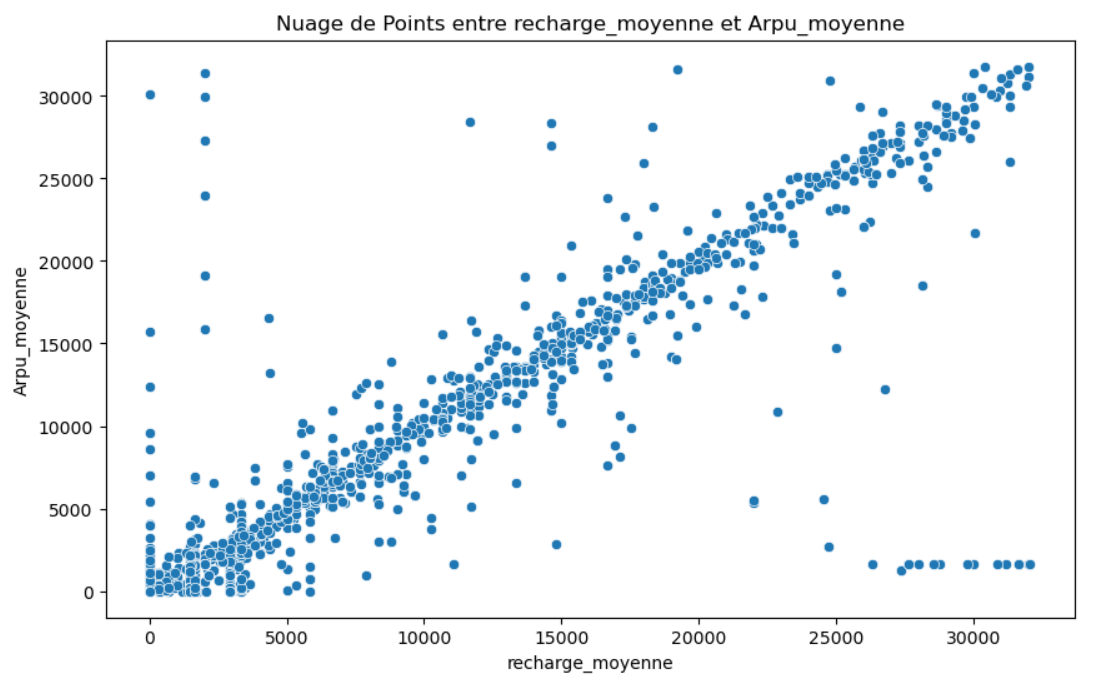
\includegraphics[width=0.6\linewidth]{capture_sas_47.png}
    \caption{Nuage de points entre \textbf{recharge\_moyenne} et \textbf{Arpu\_moyenne}}
    \label{nuage1}
\end{figure}

\noindent
Cette première figure \ref{nuage1} représente un nuage de points entre les variables \textbf{recharge\_moyenne} et \textbf{Arpu\_moyenne}. On observe une tendance positive forte, où les deux variables semblent évoluer ensemble. Cela suggère une corrélation significative.

\begin{figure}[H]
    \centering
    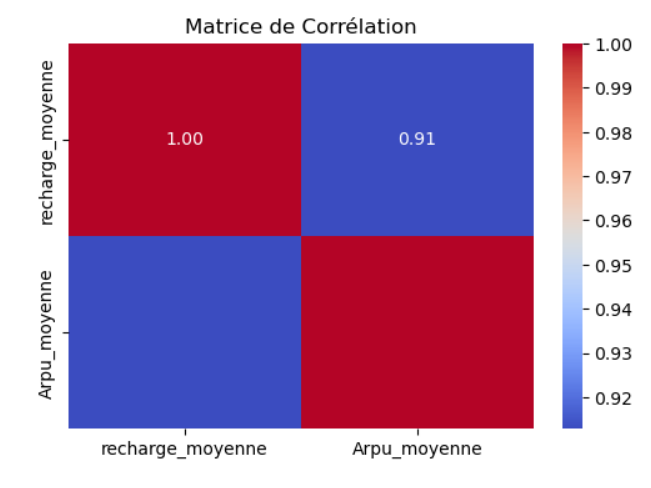
\includegraphics[width=0.6\linewidth]{capture_sas_48.png}
    \caption{Matrice de corrélation entre \textbf{recharge\_moyenne} et \textbf{Arpu\_moyenne}}
    \label{matrice1}
\end{figure}

\noindent
La matrice de corrélation dans la figure \ref{matrice1} confirme cette observation avec un coefficient de corrélation de \(0.91\), indiquant une corrélation forte et positive entre ces deux variables.\par

\textit{La figure \ref{11} de l'annexe B résume les résultats de la covariance, des tests de normalité, et du test de corrélation entre les variables \textbf{recharge\_moyenne} et \textbf{Arpu\_moyenne}. Comme les deux variables ne suivent pas une distribution normale, on a utilisé le test non paramétrique de Spearman pour évaluer la corrélation.}



\noindent
Le test de Shapiro-Wilk a montré que les deux variables \textbf{recharge\_moyenne} et \textbf{Arpu\_moyenne} ne suivent pas une distribution normale, avec des p-values très faibles (inférieures à 0.05). Par conséquent, le test non paramétrique de Spearman a été utilisé, et il a révélé une corrélation positive et forte entre ces deux variables (\textbf{r = 0.9450}, \textbf{p-value = 0.0000}). Cela signifie que lorsque \textbf{recharge\_moyenne} augmente, \textbf{Arpu\_moyenne} tend également à augmenter.

\begin{figure}[H]
    \centering
    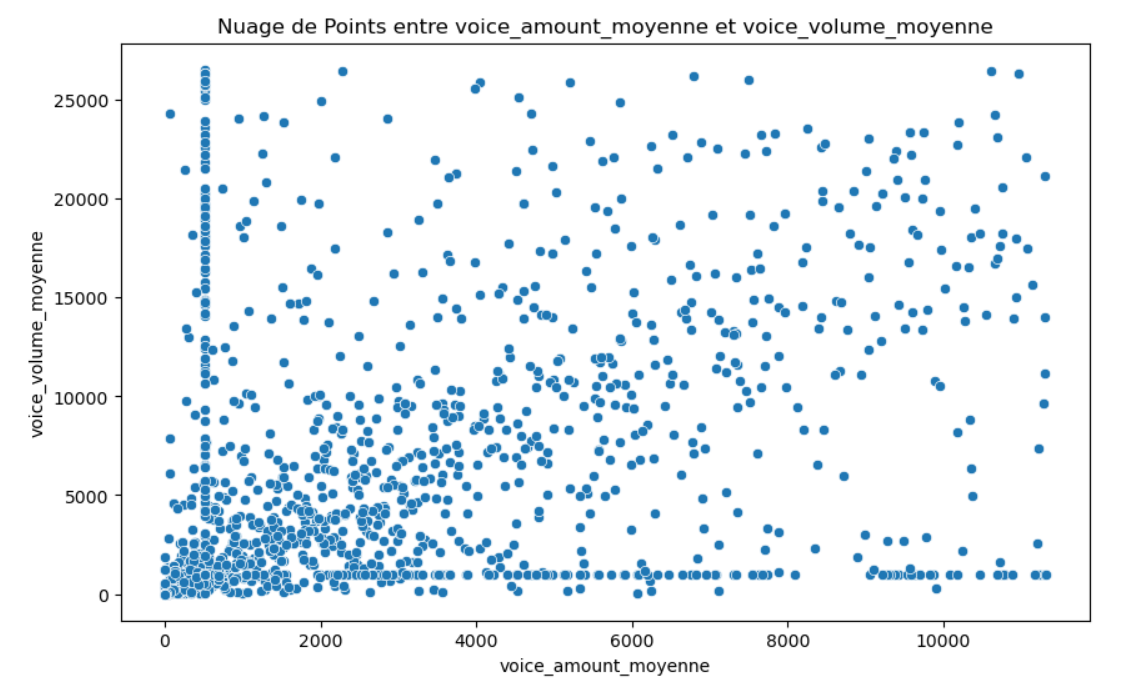
\includegraphics[width=0.6\linewidth]{capture_sas_50.png}
    \caption{Nuage de points entre \textbf{voice\_volume\_moyenne} et \textbf{voice\_amount\_moyenne}}
    \label{nuage4}
\end{figure}

\noindent
La figure \ref{nuage4} montre un nuage de points entre les variables \textbf{voice\_volume\_moyenne} et \textbf{voice\_amount\_moyenne}. Bien que la tendance soit visible, la relation reste modérée.

\begin{figure}[H]
    \centering
    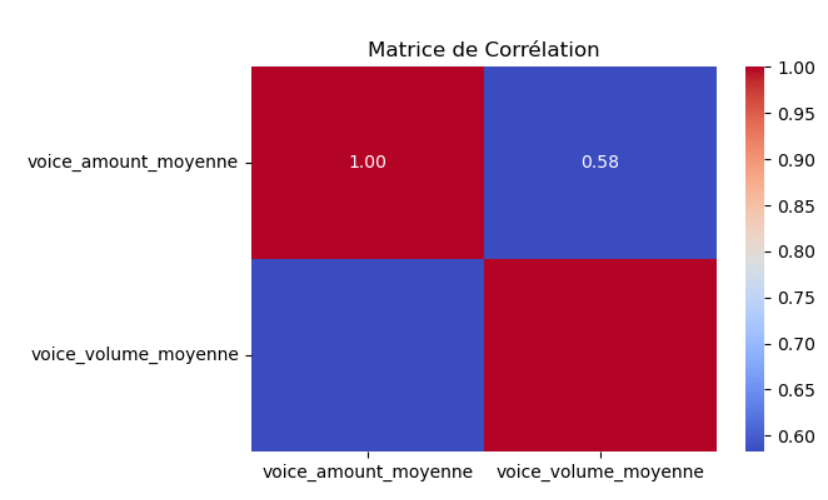
\includegraphics[width=0.6\linewidth]{capture_sas_51.png}
    \caption{Matrice de corrélation entre \textbf{voice\_volume\_moyenne} et \textbf{voice\_amount\_moyenne}}
    \label{matrice4}
\end{figure}

\noindent
La matrice de corrélation dans la figure \ref{matrice4} montre un coefficient de corrélation de \(0.58\), ce qui suggère une relation modérée entre ces deux variables.

\noindent
Les résultats des tests de Shapiro-Wilk montrent que les deux variables ne suivent pas une distribution normale, avec des p-values inférieures à 0.05. Le test de Spearman a révélé une corrélation modérée mais significative (\textbf{r = 0.58}, \textbf{p-value = 0.0000}). Cela indique que les deux variables ont tendance à augmenter ensemble, bien que la relation soit modérée.

\subsubsection*{Conclusion }

Les résultats de l'analyse des corrélations révèlent que plusieurs variables quantitatives présentent des relations significatives. Par exemple, la corrélation entre \textbf{recharge moyenne} et \textbf{ARPU} est forte avec un coefficient de \(r = 0.91\), ce qui suggère qu'une augmentation de la recharge moyenne est associée à une augmentation de l'ARPU. De même, la \textbf{voice\_volume\_moyenne} et la \textbf{voice\_amount\_moyenne} montrent également une corrélation positive avec \(r = 0.58\), reflétant une relation modérée entre ces deux variables.
Certaines relations, comme entre \textbf{recharge moyenne} et \textbf{activation\_days}, montrent une faible corrélation négative (\(r = -0.25\)), suggérant une tendance inverse entre l'ancienneté du client et la fréquence des recharges. D'autres variables, telles que \textbf{nbre\_sms\_moyenne} et \textbf{recharge\_moyenne}, affichent une corrélation positive modérée (\(r = 0.77\)).

En général, les corrélations entre les variables de consommation, telles que la \textbf{mou moyenne} ou le \textbf{data volume}, sont positives et significatives, tandis que les variables temporelles montrent un impact moindre ou négatif.

\textbf{2. Variable quantitative VS Variable qualitative:}

on va maintenant analyser les corrélations entre les variables explicatives quantitatives et qualitatives afin de comprendre leur interdépendance et leur impact potentiel sur les résultats.

Pour cette section, nous analysons les relations entre les variables explicatives quantitatives et qualitatives en utilisant les tests ANOVA et Kruskal-Wallis. Voici un exemple illustré par la figure ci-dessous.

\begin{figure}[H]
    \centering
    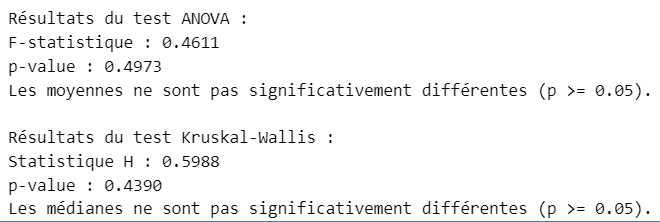
\includegraphics[width=0.7\linewidth]{capture_sas_36.png}
    \caption{Tests ANOVA/Kruskal-Wallis entre \textbf{mou\_moyenne} et \textbf{Flag\_4g\_binary}}
    \label{flag4g_mou}
\end{figure}

La figure \ref{flag4g_mou} présente l'analyse de \textbf{mou\_moyenne} selon la variable qualitative \textbf{Flag\_4g\_binary}. Les résultats des tests ANOVA et Kruskal-Wallis montrent des différences significatives entre les groupes (\textbf{p-value} < 0.05), indiquant que les utilisateurs du \textbf{Flag 4G} consomment significativement plus de minutes (\textbf{mou\_moyenne}) que les non-utilisateurs.

Dans cet exemple, nous observons que l'accès à la 4G semble être associé à une augmentation de la consommation de minutes, ce qui suggère une corrélation significative entre ces variables.

\subsection*{Conclusion }
La même méthodologie a été appliquée aux combinaisons de variables quantitatives et qualitatives. Voici quelques résultats obtenus : des différences significatives ont été observées entre \textbf{activation\_days} et \textbf{flag\_smartphone} (ANOVA p = 0.0232, Kruskal-Wallis p = 0.0006), indiquant une variation selon l'utilisation du smartphone. Concernant \textbf{recharge\_moyenne} et \textbf{Number\_of\_reactivation}, des différences significatives ont également été notées (ANOVA p = 0.0164, Kruskal-Wallis p = 0.0000), avec une recharge moyenne plus élevée pour les utilisateurs réactivés. 

Par ailleurs, \textbf{mou\_moyenne} montre des différences très significatives avec \textbf{Number\_of\_reactivation} (ANOVA p = 0.0000, Kruskal-Wallis p = 0.0000), illustrant une consommation plus importante pour les utilisateurs réactivés. Enfin, le nombre moyen de recharges (\textbf{nbre\_recharges\_moyenne}) est également significatif pour \textbf{Number\_of\_reactivation} (ANOVA p = 0.0000, Kruskal-Wallis p = 0.0000), ces utilisateurs ayant un nombre moyen de recharges plus élevé.

Ces analyses soulignent des associations importantes entre des variables qualitatives comme \textbf{flag\_smartphone} et \textbf{Number\_of\_reactivation} et des variables quantitatives telles que \textbf{mou\_moyenne} et \textbf{recharge\_moyenne}, ce qui peut guider la modélisation future.

% \subsubsection{Visualisation Tridimensionnelle des Relations}

% Cette section explore les relations entre les variables continues (\textbf{recharge\_moyenne}, \textbf{Arpu\_moyenne}, \textbf{mou\_moyenne}, \textbf{nbre\_sms\_moyenne}) et la variable qualitative \textbf{OSAT}, à travers des visualisations tridimensionnelles qui clarifient leur influence sur la satisfaction.


% \begin{figure}[H]
%     \centering
%     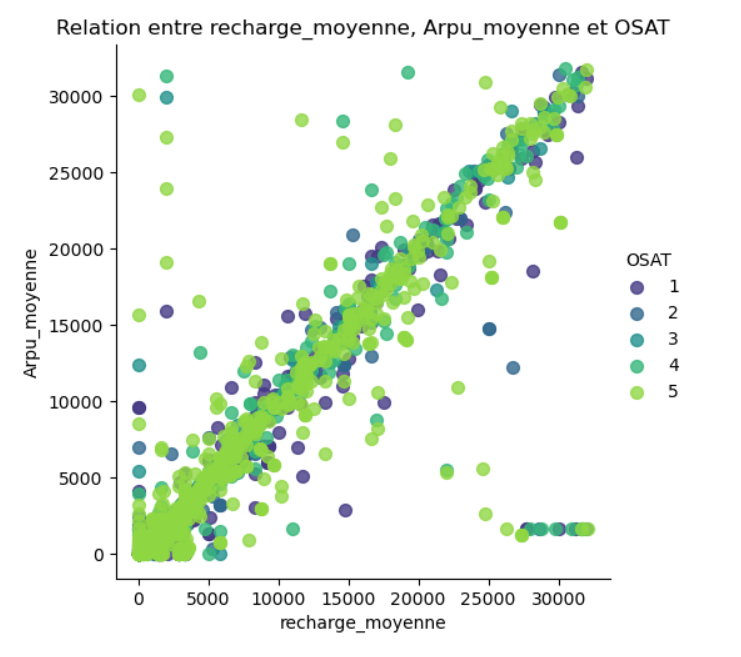
\includegraphics[width=0.5\linewidth]{capture_sas_54.png}
%     \caption{Relation entre \textbf{recharge\_moyenne}, \textbf{Arpu\_moyenne} et \textbf{osat}}
%     \label{22}
% \end{figure}

% La figure \ref{22} montre une relation positive entre \textbf{recharge\_moyenne} et \textbf{Arpu\_moyenne}, suggérant que l'augmentation des recharges est liée à une hausse de l'ARPU. Les niveaux de satisfaction (\textbf{OSAT}) révèlent une tendance où des recharges plus élevées correspondent souvent à une meilleure satisfaction (OSAT=4 ou 5). 

% Cependant, des clients avec un faible OSAT (1 ou 2) peuvent aussi avoir des recharges élevées, indiquant qu'il n'y a pas de lien systématique entre recharges élevées et satisfaction.

% \begin{figure}[H]
%     \centering
%     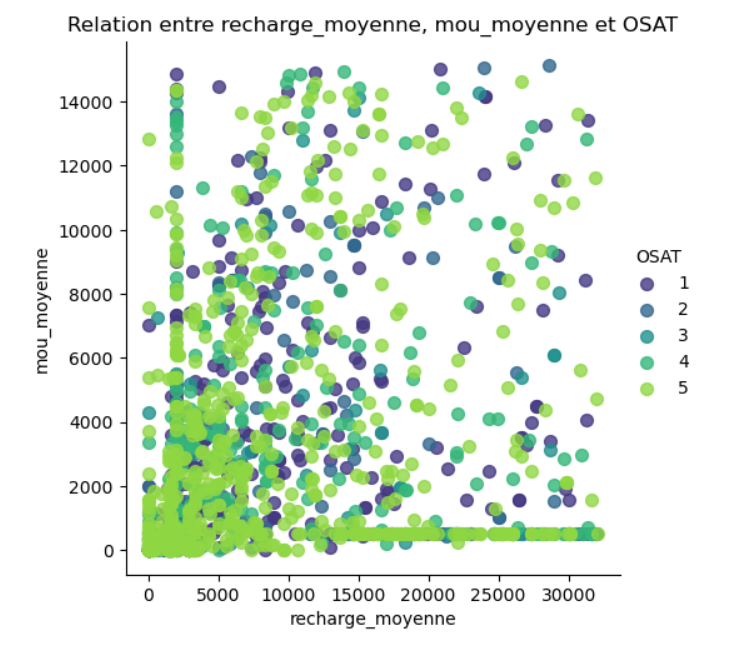
\includegraphics[width=0.5\linewidth]{capture_sas_55.png}
%     \caption{Relation entre \textbf{recharge\_moyenne}, \textbf{mou\_moyenne} et \textbf{OSAT}}
%     \label{33}
% \end{figure}

% La figure \ref{33} illustre la relation entre \textbf{recharge\_moyenne}, \textbf{mou\_moyenne} et les niveaux d'OSAT. 

% Contrairement à la forte corrélation observée dans le cas de \textbf{Arpu\_moyenne}, ici la relation entre \textbf{recharge\_moyenne} et \textbf{mou\_moyenne} est plus dispersée. Bien qu'il existe une légère tendance à l'augmentation de \textbf{mou\_moyenne} avec la hausse de \textbf{recharge\_moyenne}, cette relation n'est pas aussi marquée.

% Les niveaux de satisfaction (\textbf{OSAT}) varient également de manière irrégulière, sans tendance évidente ou forte séparation entre les différents groupes d'OSAT. Cela suggère que la variable \textbf{mou\_moyenne} n'a pas une influence directe sur le niveau de satisfaction, contrairement à d'autres variables comme \textbf{Arpu\_moyenne}.
% \subsubsection*{Relation entre \textbf{recharge\_moyenne}, \textbf{nbre\_sms\_moyenne} et \textbf{OSAT}}
% \begin{figure}[H]
%     \centering
%     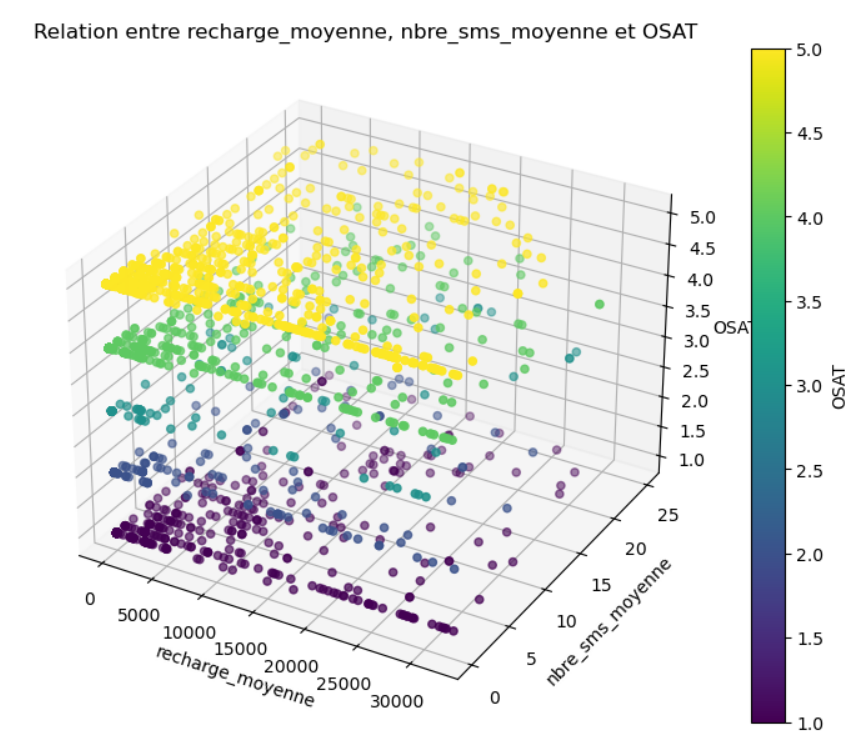
\includegraphics[width=0.6\linewidth]{capture_sas_56.png}
%     \caption{Relation entre \textbf{recharge\_moyenne}, \textbf{nbre\_sms\_moyenne} et \textbf{OSAT}}
% \end{figure}

% Cette visualisation 3D présente la relation entre \textbf{recharge\_moyenne}, \textbf{nbre\_sms\_moyenne} et \textbf{OSAT}. 

% Nous observons une légère tendance à l'augmentation des valeurs de \textbf{recharge\_moyenne} et \textbf{nbre\_sms\_moyenne}, avec une répartition ariée des niveaux de satisfaction (\textbf{OSAT}). Les utilisateurs avec un \textbf{OSAT} plus élevé semblent se concentrer dans des zones de forte \textbf{recharge\_moyenne}, tandis que les valeurs plus faibles d'\textbf{OSAT} sont davantage réparties.

% Cette visualisation tridimensionnelle permet d'explorer plus en profondeur les interactions complexes entre plusieurs variables continues et la satisfaction des utilisateurs (\textbf{OSAT}). Elle met en évidence les variables qui influencent potentiellement la satisfaction des utilisateurs, offrant ainsi des pistes d'analyse supplémentaires.

\section{Modélisation}
\subsection{Équilibrage des classes (SMOTE)}

L'équilibrage des classes de la variable cible \textbf{OSAT} a été effectué avec la méthode SMOTE (Synthetic Minority Over-sampling Technique) pour corriger la répartition initiale déséquilibrée, comme illustré par la figure \ref{smote_avant}.

\begin{figure}[H]
    \centering
    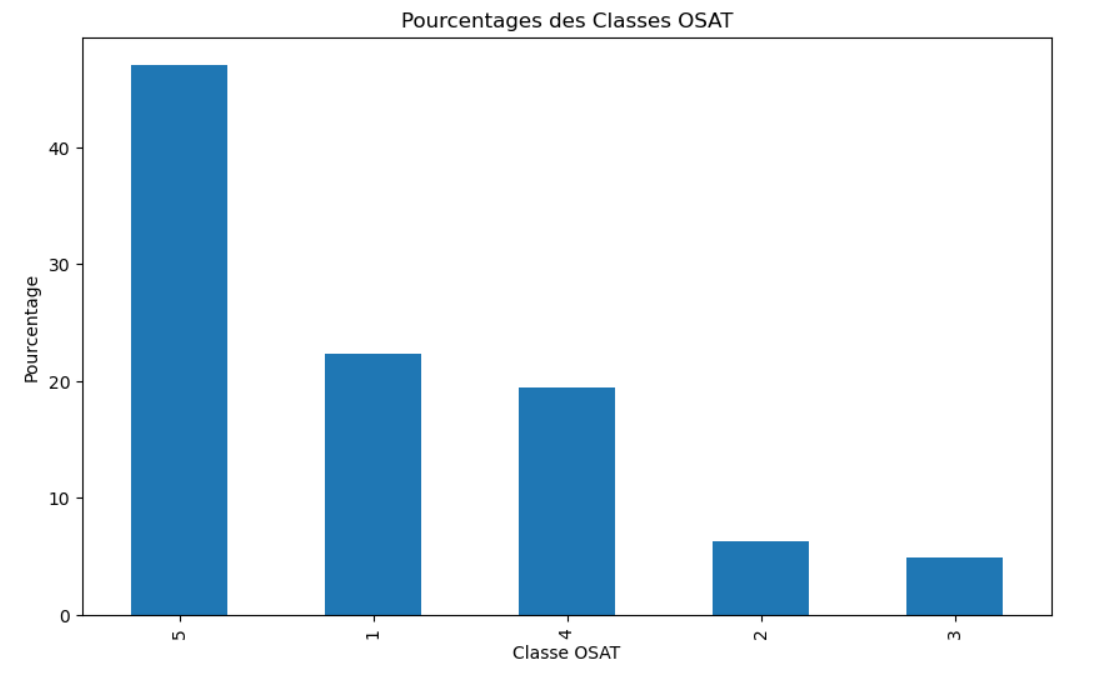
\includegraphics[width=0.7\linewidth]{capture_sas_57.png}
    \caption{Pourcentages des classes OSAT avant équilibrage}
    \label{smote_avant}
\end{figure}

Avant SMOTE, la classe 5 dominait avec 47\%, tandis que les classes 2 et 3 étaient sous-représentées. SMOTE a permis de rééquilibrer les classes en augmentant la présence des classes moins fréquentes sans suréchantillonner excessivement certaines classes.

\begin{figure}[H]
    \centering
    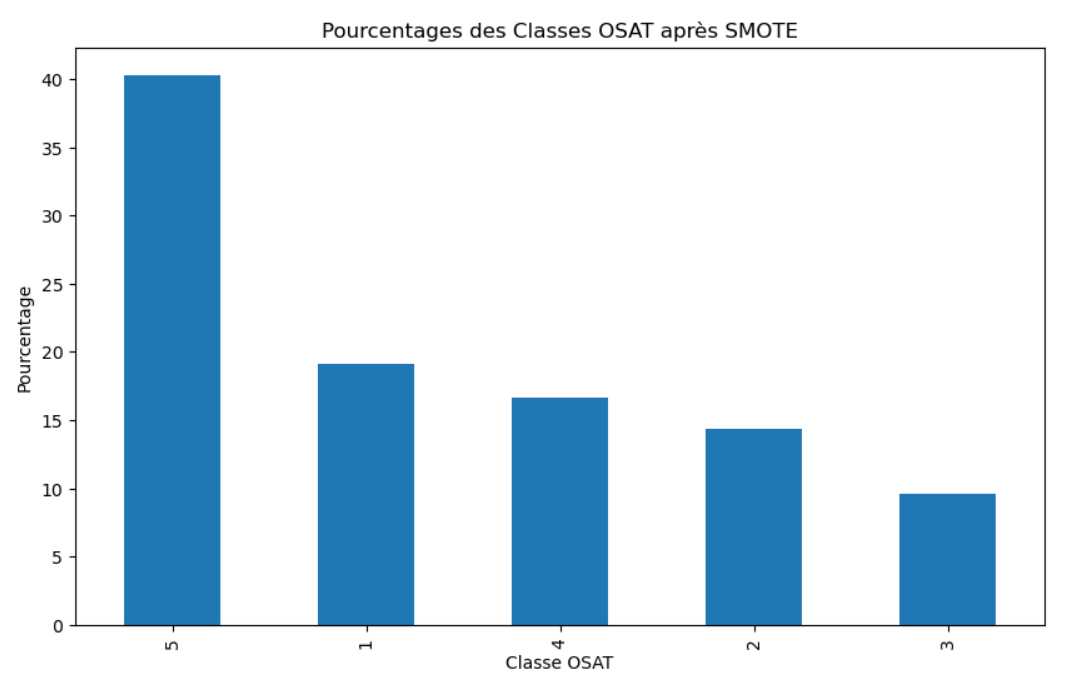
\includegraphics[width=0.7\linewidth]{capture_sas_59.png}
    \caption{Pourcentages des classes OSAT après équilibrage avec SMOTE}
    \label{smote_aprés}
\end{figure}

Après SMOTE (figure \ref{smote_aprés}), les classes sont réparties de façon plus homogène, réduisant le biais en faveur des classes majoritaires et améliorant la modélisation. Les nouvelles proportions sont :

\textbf{Classe 5}: 40.28\%, \textbf{Classe 1}: 19.15\%, \textbf{Classe 4}: 16.63\%, \textbf{Classe 2}: 14.35\%, \textbf{Classe 3}: 9.56\%.

Cette répartition équilibrée permet un jeu de données plus adapté à la modélisation et à une meilleure interprétation des résultats finaux.

\subsection{Sélection des caractéristiques}
Trois méthodes ont été appliquées pour la sélection des caractéristiques : \textbf{RFE (Recursive Feature Elimination)}, \textbf{SelectKBest}, et les \textbf{importances des caractéristiques à partir de Random Forest}. Ces méthodes permettent d'identifier les variables explicatives ayant le plus grand impact sur la prédiction de la variable cible \textbf{OSAT}. 

\textit{Le code utilisé pour effectuer cette sélection est disponible en annexe, voir Figure \ref{code_features_Selection}.}

\textbf{RFE :} La méthode RFE avec un classificateur Random Forest a identifié \textbf{recharge\_moyenne}, \textbf{data\_amount\_moyenne}, et \textbf{voice\_amount\_moyenne} comme les variables les plus pertinentes (rang 1). 

\begin{figure}[H]
    \centering
    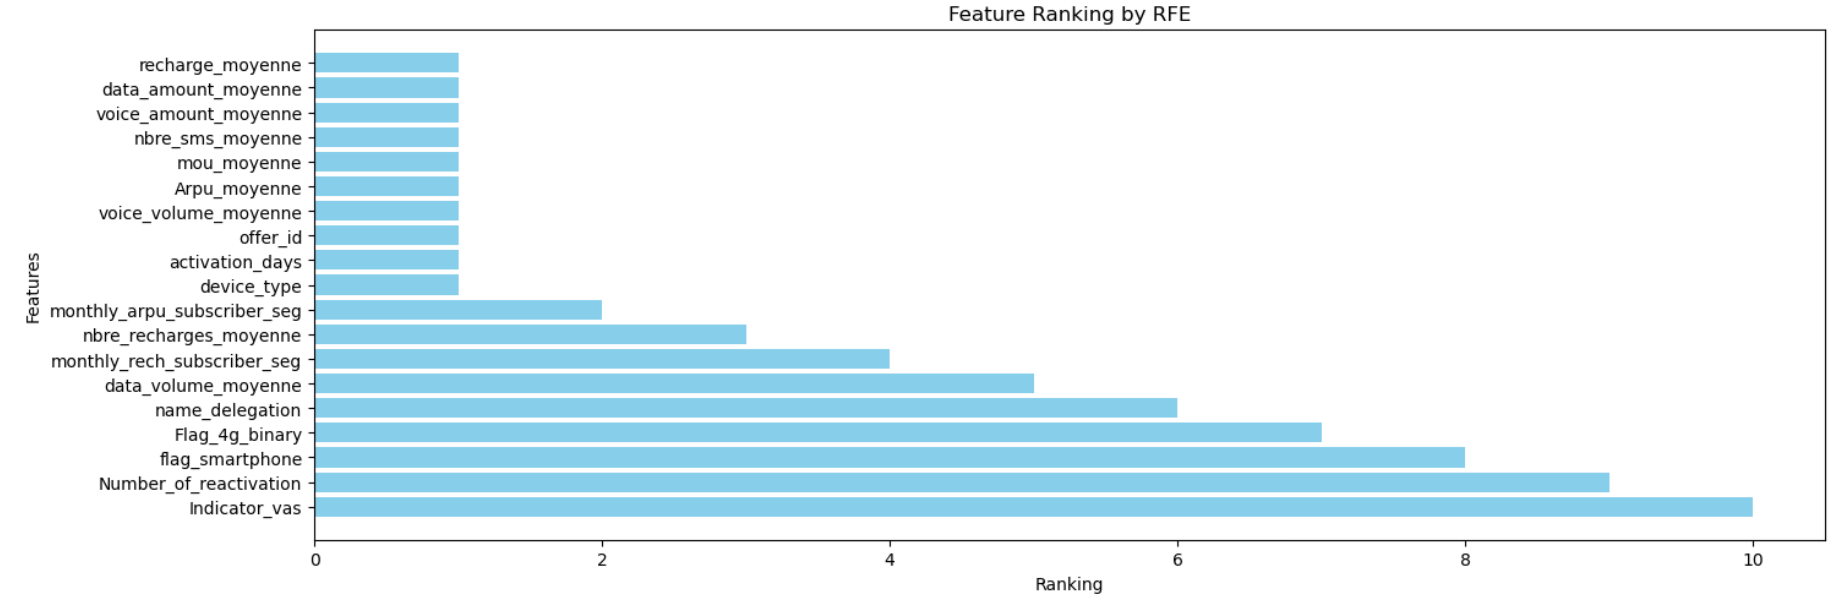
\includegraphics[width=0.8\linewidth]{capture_sas_65.png}
    \caption{Classement des caractéristiques par RFE}
\end{figure}

\textbf{SelectKBest :} Cette méthode a sélectionné des variables en fonction de leur variance expliquée. Les variables les plus influentes sont \textbf{flag\_smartphone} (score de 7.21), \textbf{recharge\_moyenne} (6.39), et \textbf{data\_amount\_moyenne} (6.38). D'autres variables importantes incluent :
\textbf{Flag\_4g\_binary} (6.12), \textbf{Arpu\_moyenne} (5.61), \textbf{voice\_volume\_moyenne} (5.43), et \textbf{monthly\_arpu\_subscriber\_seg} (5.23).

\begin{figure}[H]
    \centering
    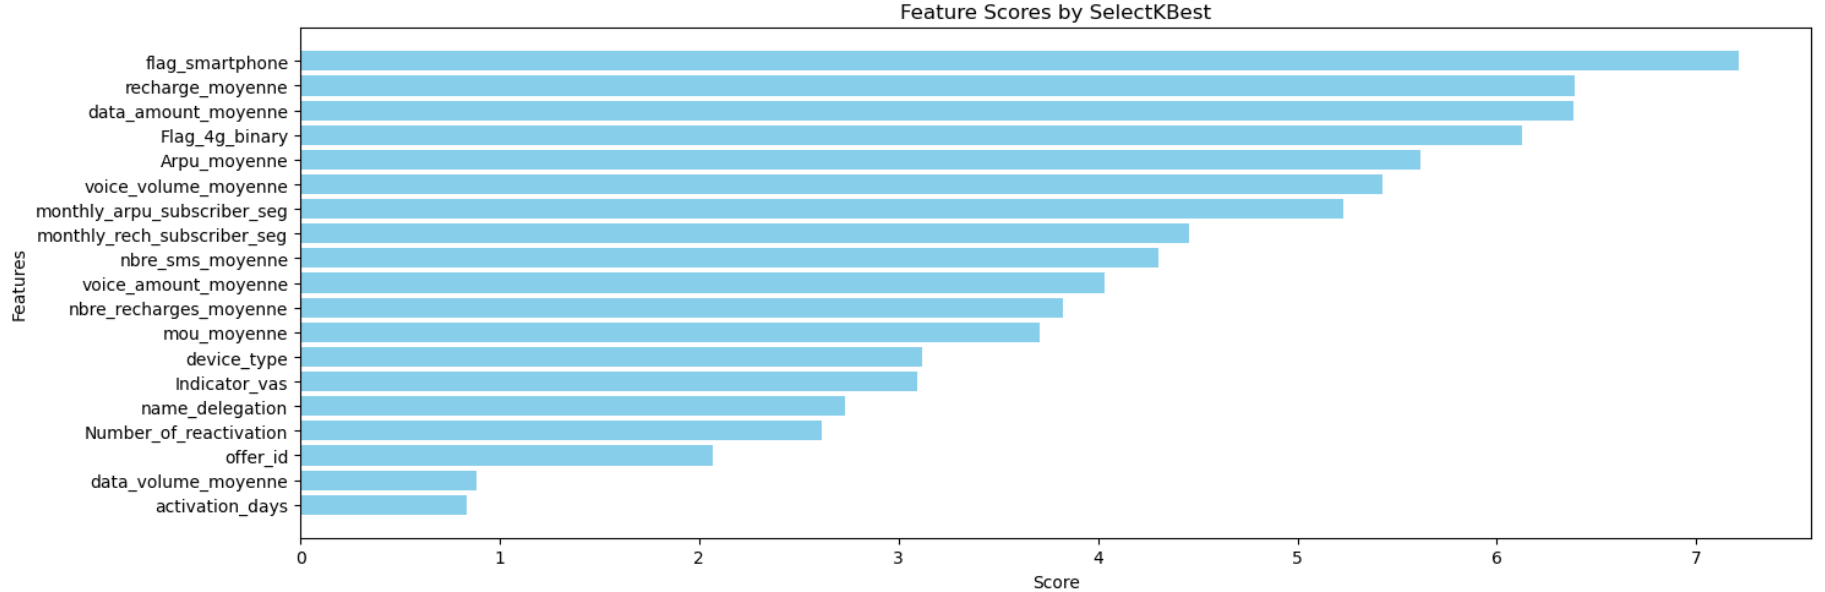
\includegraphics[width=0.8\linewidth]{capture_sas_66.png}
    \caption{Scores des caractéristiques par SelectKBest}
\end{figure}

\textbf{Random Forest :} L'analyse d'importance des caractéristiques a révélé que \textbf{activation\_days} (0.29) est la variable la plus influente, suivie par \textbf{offer\_id} (0.086) et \textbf{voice\_volume\_moyenne} (0.075). Les autres variables importantes incluent \textbf{voice\_amount\_moyenne} (0.071), \textbf{Arpu\_moyenne} (0.061), \textbf{recharge\_moyenne} (0.061), \textbf{mou\_moyenne} (0.058), et \textbf{data\_amount\_moyenne} (0.044).

\begin{figure}[H]
    \centering
    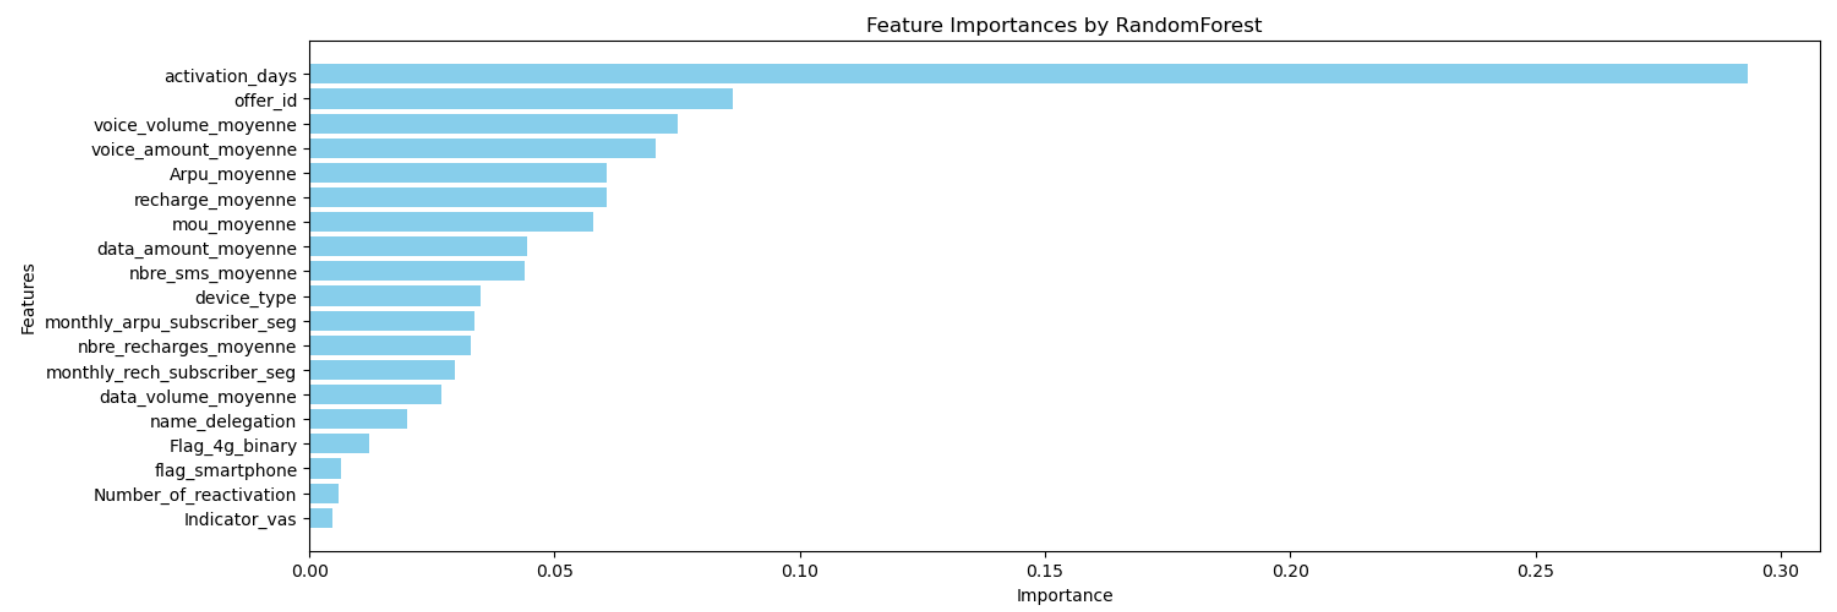
\includegraphics[width=0.8\linewidth]{capture_sas_67.png}
    \caption{Importances des caractéristiques par Random Forest}
\end{figure}


\subsubsection*{Conclusion:}
Les méthodes de sélection des caractéristiques \textbf{RFE}, \textbf{SelectKBest}, et \textbf{Random Forest} ont permis d'identifier les variables clés pour la prédiction de \textbf{OSAT}. La figure suivante montre les caractéristiques communes aux trois méthodes, telles que \textbf{recharge\_moyenne}, \textbf{voice\_amount\_moyenne}, \textbf{mou\_moyenne}, et \textbf{activation\_days}, qui se distinguent systématiquement.

\begin{figure}[H]
    \centering
    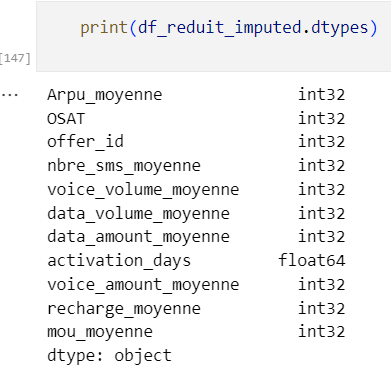
\includegraphics[width=0.4\linewidth]{capture_sas_69.png}
    \caption{Caractéristiques communes importantes entre les trois méthodes}
\end{figure}

Ce processus rigoureux a permis de définir les variables ayant un impact direct et significatif sur \textbf{OSAT}. Ces caractéristiques seront prioritaires dans les futurs modèles prédictifs pour garantir des performances optimales et des résultats fiables.

\subsection{Modélisation avec Machine Learning}

Bien que plusieurs modèles aient été testés, cette section se concentre sur l'algorithme \textbf{Random Forest}, qui a donné les meilleurs résultats. Nous avons appliqué une validation croisée, ajusté les hyperparamètres, et évalué le modèle avec des métriques telles que l'exactitude, le rappel et la courbe ROC.

\subsubsection{Prétraitement des données}
Le prétraitement a consisté à standardiser les caractéristiques avec un \textbf{StandardScaler} pour assurer une échelle comparable entre les variables. Les données ont ensuite été divisées en ensembles d'entraînement et de test (70/30) avec \textbf{train\_test\_split}.

\subsubsection{Optimisation des hyperparamètres}
L'optimisation des hyperparamètres a été réalisée avec \textbf{RandomizedSearchCV} pour explorer efficacement différentes combinaisons de paramètres, incluant \textbf{n\_estimators}, \textbf{max\_depth}, \textbf{min\_samples\_split}, \textbf{min\_samples\_leaf}, et \textbf{criterion} (\textbf{gini} ou \textbf{entropy}). Une validation croisée à 3 plis a été utilisée pour évaluer les performances.

\textit{Le code utilisé pour l'optimisation des hyperparamètres est disponible en annexe, voir Figure \ref{hyperparametres}.}

\subsubsection{Sélection des caractéristiques importantes et réentraînement du modèle}
Après avoir trouvé le meilleur modèle, les \textbf{importances des caractéristiques} ont été extraites pour identifier les variables clés dans la prédiction de \textbf{OSAT}. Seules les caractéristiques avec un seuil d'importance supérieur à 0.035 ont été retenues.

\textit{Le graphique des importances des caractéristiques est disponible en annexe, voir Figure \ref{importance}.}

Un code a également été implémenté pour optimiser le seuil de classification, en testant différents seuils afin de maximiser le compromis entre taux de vrais positifs et faux positifs. Cependant, le seuil initial de 0.035 s'est avéré plus performant en termes de précision, rappel et F1-score, offrant un meilleur équilibre sans surajuster le modèle.

Après la sélection des caractéristiques importantes, le modèle Random Forest a été réentraîné uniquement avec ces variables, sur des données standardisées, en suivant les mêmes étapes de validation croisée.

\subsubsection{Optimisation du seuil de classification}
Pour améliorer les performances du modèle, la courbe ROC a été utilisée pour déterminer le \textbf{seuil de classification optimal}, en maximisant la différence entre le taux de vrais positifs et le taux de faux positifs.

\textit{La courbe ROC et son AUC sont disponibles en annexe, voir Figure \ref{code_roc}.}

\subsubsection{Conclusion}
Le modèle Random Forest a montré de bonnes performances après optimisation. La sélection des caractéristiques et l'ajustement du seuil ont amélioré l'exactitude et la précision, avec des variables clés comme \textbf{recharge\_moyenne}, \textbf{voice\_amount\_moyenne}, et \textbf{activation\_days}.

\subsection{Modélisation avec Deep Learning}
Dans cette section, nous explorons l'application des réseaux de neurones pour la prédiction de la variable cible \textbf{osat\_binary}, à travers deux approches distinctes: \textbf{PyTorch} et \textbf{Keras/TensorFlow}. Nous détaillons le processus de modélisation, incluant la préparation des données, le choix des architectures de réseaux de neurones, et les stratégies de réglage des hyperparamètres, tout en mettant en évidence les spécificités de chaque approche.

\subsubsection{Approche PyTorch}
L'approche \textbf{PyTorch} a été choisie pour sa flexibilité. Nous avons construit un modèle de classification binaire pour prédire la satisfaction des clients (\textbf{osat\_binary}).

\textbf{1. Préparation des données:} Les données ont été standardisées et converties en tenseurs. Les \textbf{poids de classe} ont été calculés pour traiter le déséquilibre des classes. 

\textit{Le code détaillé de la préparation des données est disponible en annexe, voir Figure \ref{pytorch_code}.}

\textbf{2. Architecture du modèle:} Le modèle contient trois couches cachées avec \textbf{ReLU} et \textbf{Dropout} pour éviter le surajustement. La dernière couche utilise \textbf{sigmoïde} pour la classification binaire.

\textit{L'architecture du modèle est présentée en annexe, voir Figure \ref{model_architecture}.}

\textbf{3. Optimisation des hyperparamètres:} L'algorithme \textbf{Adam} a été utilisé avec différentes combinaisons d'hyperparamètres (\textbf{learning rate}, \textbf{batch size}, \textbf{Dropout}). Le modèle a été entraîné sur 100 époques pour garantir la convergence. 

\textit{Le processus d'optimisation des hyperparamètres est disponible en annexe, voir Figure \ref{fig_hyperparam_code}.}

\textbf{4. Sélection du meilleur modèle et évaluation:} Le modèle avec les meilleurs hyperparamètres a été sélectionné : \textbf{learning rate} de 0.01, \textbf{batch size} de 32, \textbf{Dropout} de 0.3. Il a été évalué avec des métriques telles que la précision, le rappel, le F1-score, et la matrice de confusion.

\textit{Les résultats de l'évaluation finale sont en annexe, voir Figure \ref{753}.}

\subsubsection{Approche Keras/TensorFlow}

Cette section présente trois approches pour modéliser les données avec Keras/TensorFlow : une architecture classique, une optimisation des hyperparamètres et une optimisation de l'architecture des couches.

\textbf{1. Approche Classique:} Une architecture de réseau de neurones simple avec des couches denses et des fonctions d'activation \textbf{ReLU}. Le modèle a été entraîné avec un taux d'apprentissage de \textbf{0.001}, 200 époques, et une taille de lot de 16.

\textit{L'architecture classique est disponible en annexe, voir Figure \ref{96}.}

\textbf{2. Optimisation des Hyperparamètres:} Cette approche optimise des paramètres comme le taux d'apprentissage, le \textbf{dropout}, le nombre d'unités par couche et la taille des lots. Les valeurs explorées incluent :
\textbf{learning rate} [1e-5, 1e-4, 1e-3, 1e-2], \textbf{dropout} [0.3, 0.4, 0.5], unités par couche [32, 64, 128], \textbf{batch size} [16, 32, 64], et 20 époques. Cette optimisation a amélioré les performances du modèle.

\textit{Le processus d'optimisation des hyperparamètres pour Keras est présenté en annexe, voir Figure \ref{op}.}

\textbf{3. Optimisation de l'Architecture des Couches:} L'optimisation de l'architecture des couches a exploré différentes configurations, fonctions d'activation (\textbf{ReLU}, \textbf{sigmoid}, \textbf{tanh}) et optimiseurs. Les architectures testées incluent [64], [64, 32], et [128, 64, 32], cette dernière s'avérant la plus performante avec \textbf{ReLU} pour les premières couches et \textbf{Sigmoid} pour la dernière.

\textit{Les détails de l'optimisation des couches sont en annexe, voir Figure \ref{arch}.}


\subsubsection{Conclusion}
Les approches PyTorch et Keras/TensorFlow ont permis d'explorer différentes stratégies de modélisation. PyTorch a optimisé les hyperparamètres pour de meilleures performances, tandis que Keras/TensorFlow a testé diverses configurations de modèles, incluant des réseaux standard, des optimisations d'hyperparamètres et des architectures de couches. Les résultats seront détaillés dans le prochain chapitre.

\section{Conclusion}

Ce chapitre a couvert le prétraitement des données, la sélection des caractéristiques et la modélisation avec des algorithmes de Machine Learning et Deep Learning.\\ 
Après avoir optimisé les modèles, on a retenu les meilleures configurations pour chaque méthode. Les résultats finaux des performances des modèles seront présentés dans le chapitre suivant.


% \chapter{Résultats et interprétation}
\begin{spacing}{1.2}
\minitoc
\thispagestyle{MyStyle}
% \setstretch{1.2} 
\end{spacing}
\newpage
\justifying

\setstretch{1.5} 
\section{Introduction}
Dans ce chapitre, nous présentons les résultats des modèles de machine learning et deep learning appliqués à trois datasets distincts. L'objectif est d'évaluer la performance de chaque modèle pour identifier les meilleures méthodes de classification.

Nous analyserons les résultats des modèles traditionnels (régression logistique, arbres de décision, Random Forest) ainsi que des modèles de deep learning basés sur PyTorch et Keras/TensorFlow. Une comparaison finale déterminera la meilleure approche pour la généralisation et les insights sur les facteurs influençant la satisfaction des clients.
\section{Résultats des Modèles de Machine Learning}

Plusieurs modèles de \textit{Machine Learning} ont été testés pour prédire la variable cible à partir des caractéristiques fournies. Les modèles utilisés incluent : \textbf{Régression Logistique}, \textbf{Arbre de Décision}, \textbf{Random Forest}, \textbf{AdaBoost}, \textbf{Gradient Boosting}, et un \textbf{Modèle Ensembliste}.

Ces modèles ont été entraînés et évalués sur trois jeux de données (\textit{network\_fev}, \textit{network\_may}, \textit{retail\_juin}) afin de comparer leurs performances respectives.

\subsection{Modèle de Régression Logistique}

La régression logistique est un modèle de base souvent utilisé pour la classification binaire. Nous l'avons appliqué sur les trois datasets : \textit{network\_fev}, \textit{network\_may}, et \textit{retail\_juin}, afin de fournir une première évaluation de la relation entre les variables explicatives et la variable cible.

\subsubsection{Résultats pour les trois datasets}

Les résultats obtenus avec la régression logistique sur les trois datasets sont résumés dans le tableau ci-dessous :

\begin{table}[H]
    \centering
    \begin{tabular}{|c|c|c|c|c|}
        \hline
        \textbf{Dataset} & \textbf{Exactitude} & \textbf{Précision} & \textbf{Rappel} & \textbf{F1-score} \\
        \hline
        \textit{network\_fev} & 0.52 & 0.52 & 0.52 & 0.52 \\
        \textit{network\_may} & 0.61 & 0.60 & 0.61 & 0.60 \\
        \textit{retail\_juin} & 0.66 & 0.57 & 0.66 & 0.54 \\
        \hline
    \end{tabular}
    \caption{Résultats des métriques pour le modèle de régression logistique sur les trois datasets.}
\end{table}

\subsubsection*{Figures et interprétations}
Les figures ci-dessous illustrent les matrices de confusion et les courbes ROC pour chaque dataset, permettant de visualiser la performance du modèle en termes de classification et de qualité des prédictions.

\begin{figure}[H]
    \centering
    \begin{minipage}{0.45\linewidth}
        \centering
        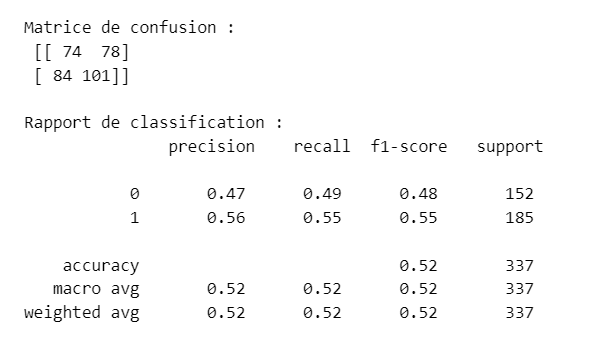
\includegraphics[width=\linewidth]{capture_modele_1.png}
        \caption{Matrice de confusion pour \textit{network\_fev}.}
        \label{eee}
    \end{minipage}
    \hfill
    \begin{minipage}{0.45\linewidth}
        \centering
        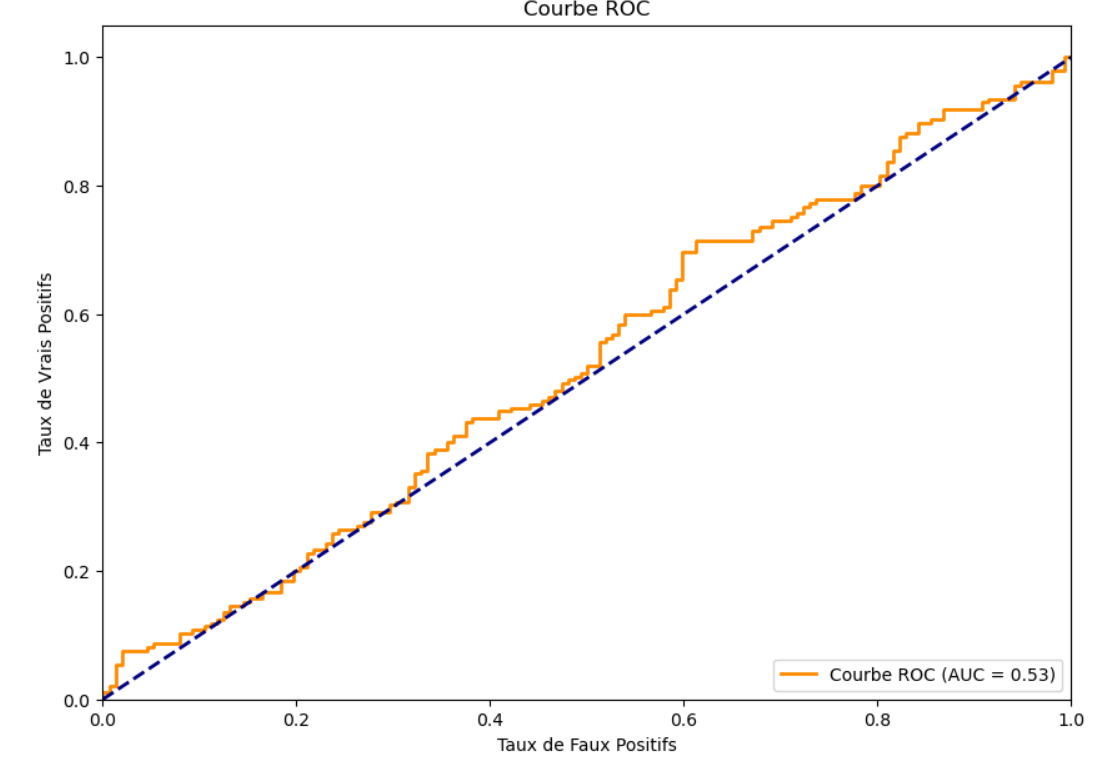
\includegraphics[width=\linewidth]{capture_modele_3.png}
        \caption{Courbe ROC pour \textit{network\_fev}.}
        \label{hhh}
    \end{minipage}
\end{figure}

\textbf{Interprétation :} Pour le dataset \textit{network\_fev}, la matrice de confusion montre une classification équilibrée entre faux positifs et vrais négatifs, mais le modèle struggle à bien différencier les classes (F1-score de 0.52). La courbe ROC de la figure \ref{hhh} affiche une AUC de 0.53, ce qui indique une performance légèrement meilleure qu'une prédiction aléatoire.

\begin{figure}[H]
    \centering
    \begin{minipage}{0.45\linewidth}
        \centering
        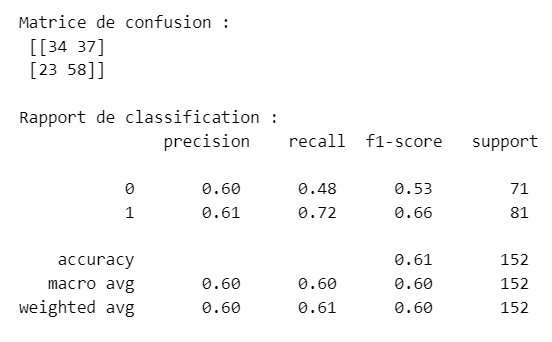
\includegraphics[width=\linewidth]{capture_modele_4.png}
        \caption{Matrice de confusion pour \textit{network\_may}.}
        \label{mmm}
    \end{minipage}
    \hfill
    \begin{minipage}{0.45\linewidth}
        \centering
        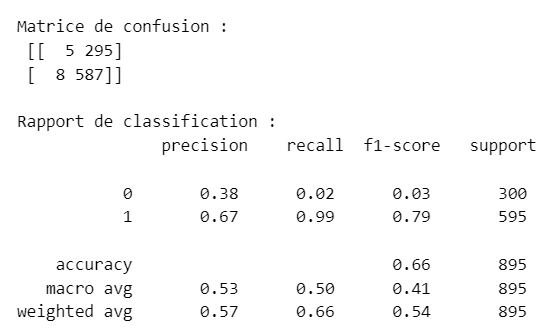
\includegraphics[width=\linewidth]{capture_modele_20.png}
        \caption{Matrice de confusion pour \textit{retail\_juin}.}
        \label{nnn}
    \end{minipage}
\end{figure}

\textbf{Interprétation :} Pour \textit{network\_may}, la précision est plus élevée (0.61), avec un meilleur équilibre entre faux positifs et vrais positifs. Enfin, la matrice de confusion pour \textit{retail\_juin} montre une performance légèrement améliorée par rapport aux autres datasets. Avec une exactitude de 0.66 et un F1-score de 0.54, le modèle a réussi à mieux classer les observations de la classe 1 (rappel de 0.99), mais continue à avoir des difficultés avec la classe 0 (F1-score de 0.03).

\subsubsection{Comparaison des résultats entre les trois datasets}

Les performances du modèle de régression logistique varient significativement entre les trois datasets.

\textbf{Performance globale :} Le dataset \textit{network\_may} a obtenu les meilleurs résultats avec une précision de 0.61 et un F1-score de 0.60. Cette meilleure performance pourrait être liée à une complexité moindre des données ou à une distribution de classes plus favorable. En revanche, les datasets \textit{network\_fev} et \textit{retail\_juin} ont montré des performances légèrement inférieures avec des F1-scores de 0.52 et 0.54 respectivement.

\textbf{Taille des datasets :} Malgré la taille plus importante de \textit{retail\_juin} (2800 lignes), les performances ne sont pas nettement meilleures. L'exactitude est légèrement plus élevée (0.66), mais le modèle peine à classer correctement la classe 0, avec un F1-score très faible pour cette classe.

\textbf{Équilibre des classes :} Le modèle montre une difficulté à distinguer les classes, particulièrement dans \textit{retail\_juin}, où la classe 0 est mal représentée dans les prédictions (rappel de 0.02). Cela suggère une tendance à privilégier la classe majoritaire, un problème courant avec des datasets déséquilibrés.

En conclusion, bien que la régression logistique ait donné des résultats modérés sur l'ensemble des datasets, elle semble mieux s'adapter à \textit{network\_may}. Les résultats obtenus sur les datasets plus grands comme \textit{retail\_juin} suggèrent qu'un modèle plus complexe pourrait être nécessaire pour capturer les relations non linéaires présentes dans les données.

\subsection{Modèle Arbre de Décision}

L'arbre de décision est un modèle non paramétrique utilisé pour la classification. Il est souvent apprécié pour sa simplicité d'interprétation et son efficacité dans la capture des relations non linéaires dans les données. on a appliqué ce modèle sur les trois datasets : \textit{network\_fev}, \textit{network\_may}, et \textit{retail\_juin}.

\subsubsection{Résultats pour les trois datasets}

Les résultats obtenus avec l'arbre de décision sur les trois datasets sont résumés dans le tableau ci-dessous :

\begin{table}[H]
    \centering
    \begin{tabular}{|c|c|c|c|c|}
        \hline
        \textbf{Dataset} & \textbf{Exactitude} & \textbf{Précision} & \textbf{Rappel} & \textbf{F1-score} \\
        \hline
        \textit{network\_fev} & 0.57 & 0.56 & 0.57 & 0.56 \\
        \textit{network\_may} & 0.63 & 0.63 & 0.63 & 0.62 \\
        \textit{retail\_juin} & 0.62 & 0.62 & 0.62 & 0.62 \\
        \hline
    \end{tabular}
    \caption{Résultats des métriques pour le modèle d'Arbre de Décision sur les trois datasets.}
\end{table}
\subsubsection*{Figures et interprétations}

Les matrices de confusion et courbes ROC ci-dessous permettent de visualiser la performance du modèle sur chaque dataset.

\begin{figure}[H]
    \centering
    \begin{minipage}{0.45\textwidth}
        \centering
        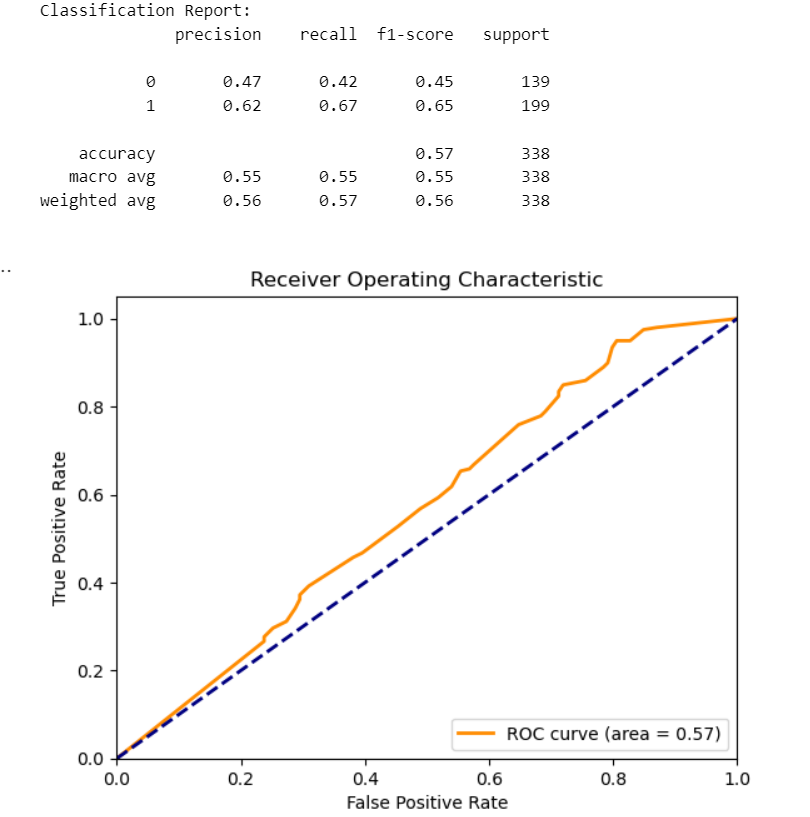
\includegraphics[width=\linewidth]{capture_modele_6.png}
        \caption{Matrice de confusion pour \textit{network\_fev}.}
    \end{minipage}
    \hfill
    \begin{minipage}{0.45\textwidth}
        \centering
        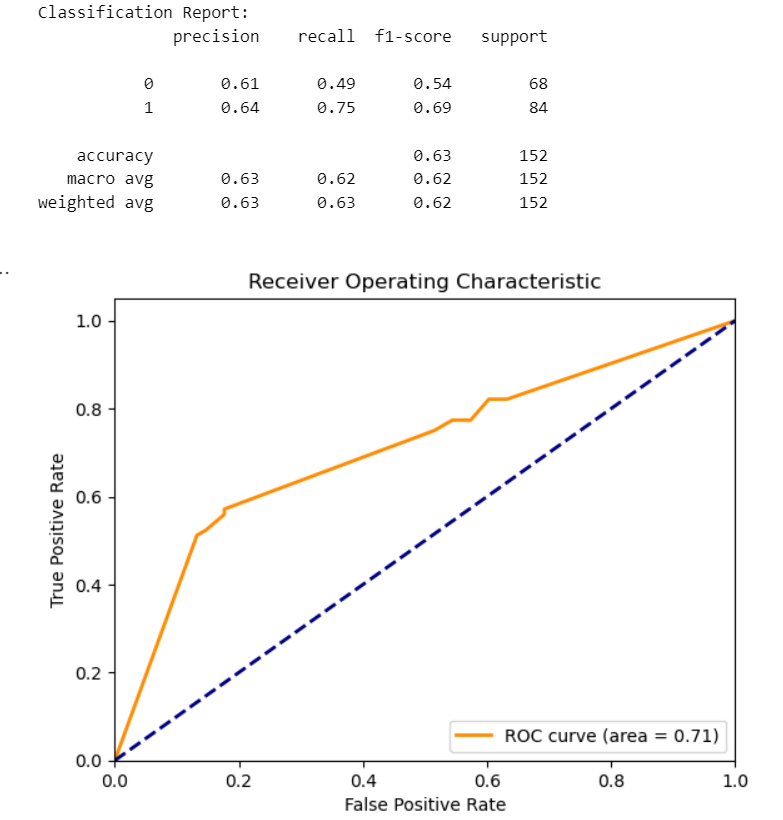
\includegraphics[width=\linewidth]{capture_modele_7.png}
        \caption{Matrice de confusion pour \textit{network\_may}.}
    \end{minipage}
\end{figure}

\begin{figure}[H]
    \centering
    \begin{minipage}{0.45\textwidth}
        \centering
        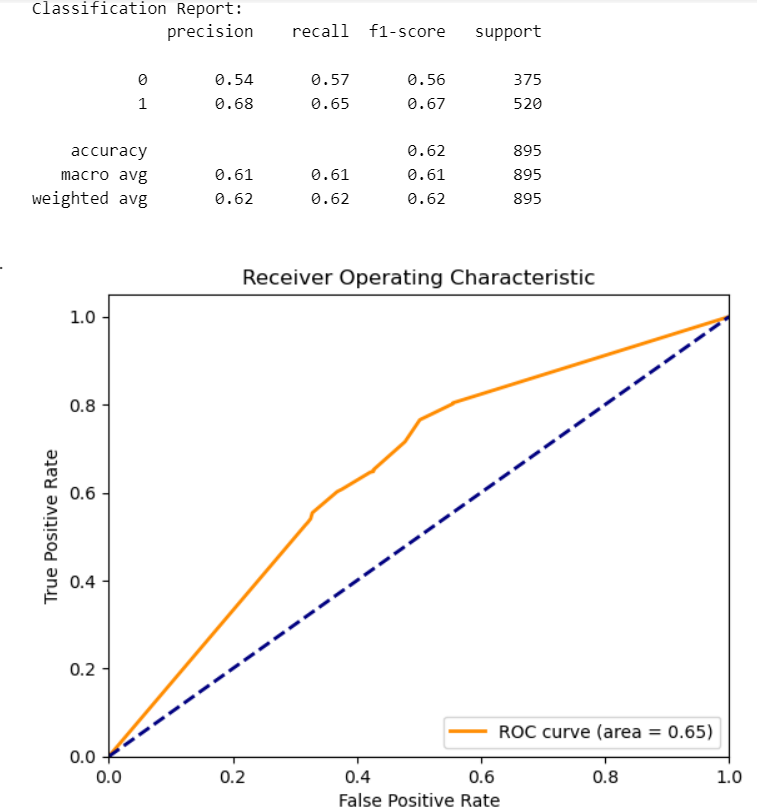
\includegraphics[width=\linewidth]{capture_modele_8.png}
        \caption{Matrice de confusion pour \textit{retail\_juin}.}
    \end{minipage}
\end{figure}

\textbf{Interprétations :}
\begin{itemize}
    \item \textbf{\textit{network\_fev} :} Le modèle atteint une exactitude de 0.57 et un F1-score de 0.56. La courbe ROC montre une AUC de 0.57, indiquant des performances moyennes.
    \item \textbf{\textit{network\_may} :} Une meilleure performance avec une exactitude de 0.63 et une AUC de 0.71, suggérant une meilleure capacité de discrimination.
    \item \textbf{\textit{retail\_juin} :} Performance similaire avec une exactitude de 0.62 et une AUC de 0.65, montrant une bonne capacité de classification.
\end{itemize}

\subsubsection{Comparaison des résultats entre les trois datasets}

Les résultats du modèle d'arbre de décision appliqué aux trois datasets montrent des différences modérées dans les performances.

\textbf{Performance globale:} Le modèle obtient de meilleures performances sur \textit{network\_may} (AUC de 0.71 et F1-score de 0.62) par rapport aux autres datasets, tandis que \textit{network\_fev} obtient des résultats plus faibles avec une AUC de 0.57 et un F1-score de 0.56. \textit{retail\_juin} a également de bons résultats avec un F1-score de 0.62.

\textbf{Taille des datasets:} Comme pour la régression logistique, le plus grand dataset (\textit{retail\_juin}) n'a pas montré d'amélioration significative par rapport à \textit{network\_may}, ce qui suggère que la taille du dataset n'est pas le seul facteur influençant la performance de l'arbre de décision.

\textbf{Equilibre entre les classes:} Le modèle semble bien distinguer les classes sur \textit{network\_may} et \textit{retail\_juin}, mais a plus de difficulté avec \textit{network\_fev}, où la proportion de faux positifs et de faux négatifs est plus importante.

En conclusion, l'arbre de décision semble mieux s'adapter aux données moins complexes de \textit{network\_may}, tandis que ses performances sur \textit{network\_fev} et \textit{retail\_juin} restent modérées.

\subsection{Modèle de Random Forest}

Après avoir constaté que le modèle d’arbre de décision avait fourni des résultats meilleurs que la régression logistique, on a choisi d’implémenter un modèle de Random Forest afin d’améliorer davantage la performance du modèle de classification. Ce modèle permet de capturer plus efficacement la complexité des données en combinant plusieurs arbres de décision.

\subsubsection{Résultats pour les trois datasets}

Les résultats obtenus avec Random Forest sur les trois datasets sont résumés dans le tableau ci-dessous :

\begin{table}[H]
    \centering
    \begin{tabular}{|c|c|c|c|c|}
        \hline
        \textbf{Dataset} & \textbf{Exactitude} & \textbf{Précision} & \textbf{Rappel} & \textbf{F1-score} \\
        \hline
        \textit{network\_fev} & 0.67 & 0.69 & 0.67 & 0.64 \\
        \textit{network\_may} & 0.74 & 0.77 & 0.76 & 0.76 \\
        \textit{retail\_juin} & 0.74 & 0.73 & 0.82 & 0.77 \\
        \hline
    \end{tabular}
    \caption{Résultats des métriques pour le modèle de Random Forest sur les trois datasets.}
\end{table}

\subsubsection*{Figures et interprétations}

Les figures ci-dessous illustrent les matrices de confusion et les courbes ROC pour chaque dataset, permettant de visualiser la performance du modèle en termes de classification et de qualité des prédictions.

\begin{figure}[H]
    \centering
    \begin{minipage}{0.45\linewidth}
        \centering
        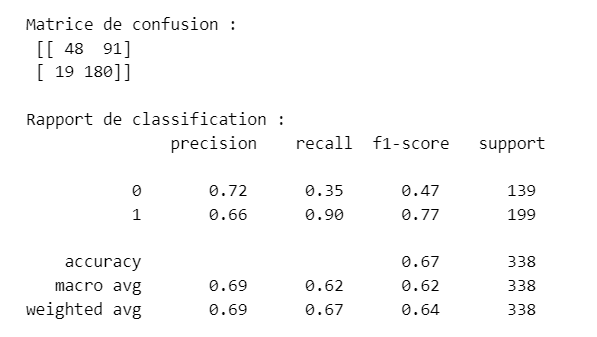
\includegraphics[width=\linewidth]{capture_modele_9.png}
        \caption{Matrice de confusion pour \textit{network\_fev}.}
    \end{minipage}
    \hfill
    \begin{minipage}{0.45\linewidth}
        \centering
        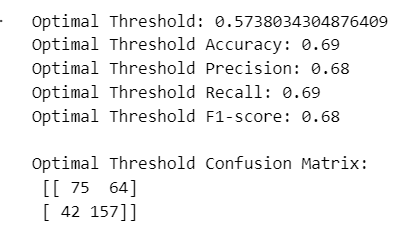
\includegraphics[width=\linewidth]{capture_modele_10.png}
        \caption{Courbe ROC pour \textit{network\_fev}.}
    \end{minipage}
\end{figure}

\textbf{Interprétation :} Le modèle montre une amélioration par rapport à l'arbre de décision sur \textit{network\_fev}, avec une exactitude de 0.67 et un F1-score de 0.64. La courbe ROC affiche une AUC de 0.79, ce qui montre une meilleure capacité de discrimination par rapport aux modèles précédents.

\begin{figure}[H]
    \centering
    \begin{minipage}{0.45\linewidth}
        \centering
        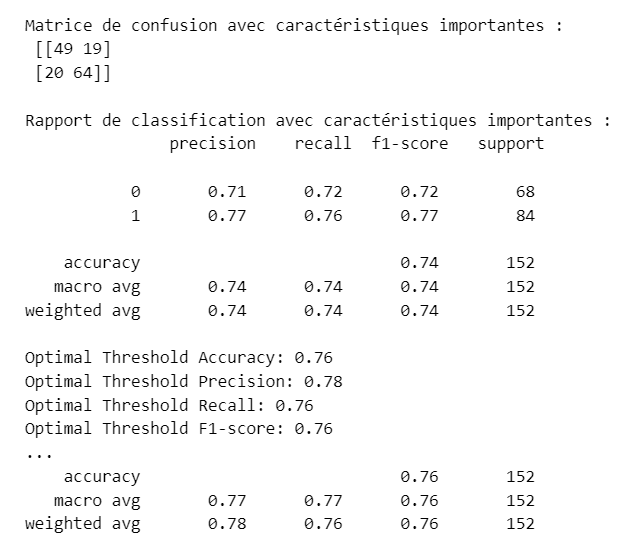
\includegraphics[width=\linewidth]{capture_modele_11.png}
        \caption{Matrice de confusion pour \textit{network\_may}.}
    \end{minipage}
    \hfill
    \begin{minipage}{0.45\linewidth}
        \centering
        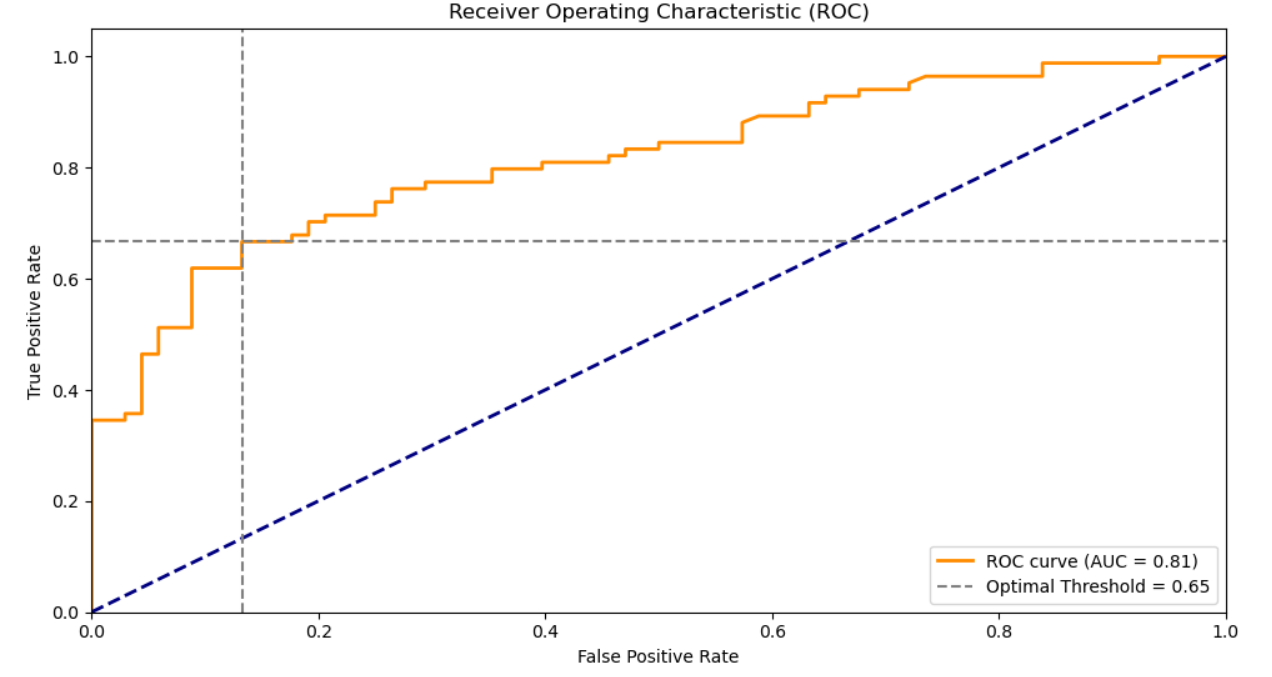
\includegraphics[width=\linewidth]{capture_modele_40.png}
        \caption{Courbe ROC pour \textit{network\_may}.}
        \label{fig:roc_may_rf}
    \end{minipage}
\end{figure}

\textbf{Interprétation :} Sur \textit{network\_may}, le modèle Random Forest performe bien avec une exactitude de 0.74 et un F1-score de 0.76. La courbe ROC affiche une AUC de 0.81, avec un seuil optimal de 0.65.

\begin{figure}[H]
    \centering
    \begin{minipage}{0.45\linewidth}
        \centering
        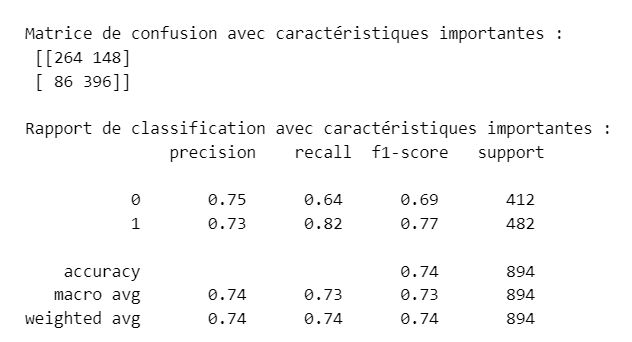
\includegraphics[width=\linewidth]{capture_modele_14.png}
        \caption{Matrice de confusion pour \textit{retail\_juin}.}
    \end{minipage}
    \hfill
    \begin{minipage}{0.45\linewidth}
        \centering
        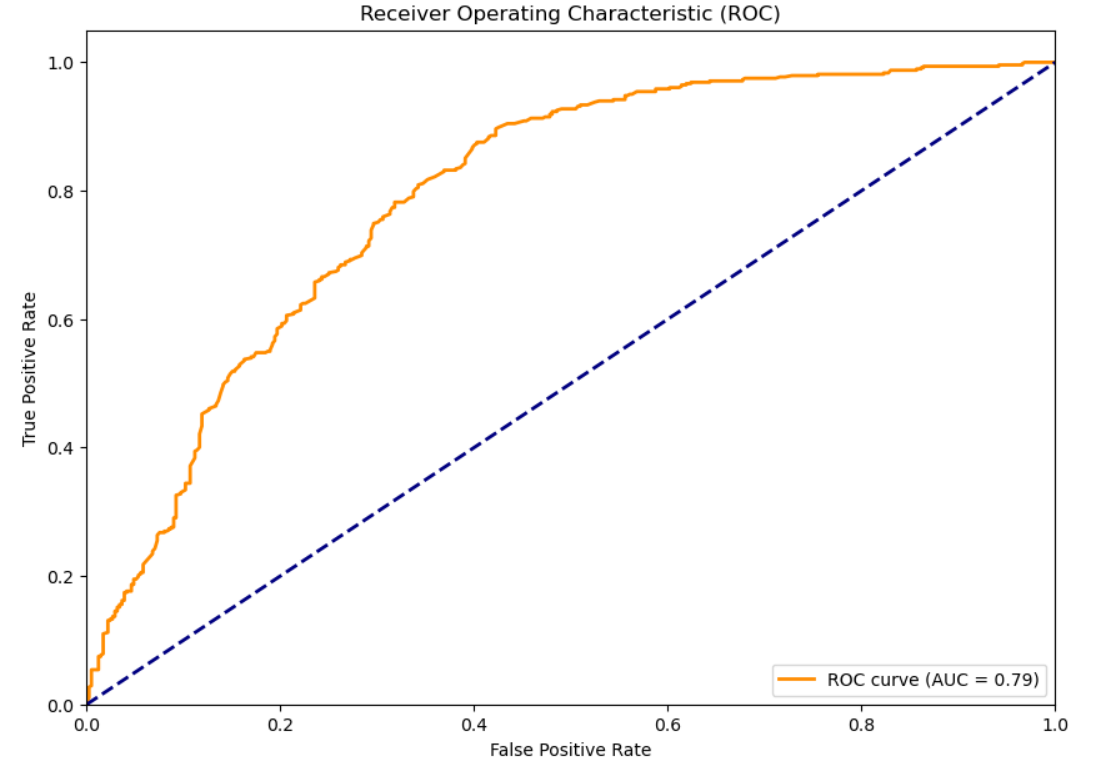
\includegraphics[width=\linewidth]{capture_modele_15.png}
        \caption{Courbe ROC pour \textit{retail\_juin}.}
        \label{fig:roc_juin_rf}
    \end{minipage}
\end{figure}

\textbf{Interprétation :} Sur \textit{retail\_juin}, le modèle atteint une exactitude de 0.74, un rappel de 0.82 et un F1-score de 0.77. La courbe ROC montre une AUC de 0.79, ce qui indique que le modèle performe bien sur ce dataset.
\subsubsection{Sélection automatique du seuil d'importance}

Pour optimiser la performance du modèle et réduire la complexité, une sélection automatique des caractéristiques importantes a été implémentée. Cette approche ajuste un seuil d'importance variable pour maintenir une bonne performance tout en simplifiant le modèle.

Le processus suivi :
\begin{itemize}
    \item Tester différents seuils d'importance pour sélectionner les caractéristiques les plus pertinentes.
    \item Réentraîner le modèle avec les caractéristiques sélectionnées pour chaque seuil.
    \item Mesurer l'exactitude pour déterminer le meilleur seuil.
\end{itemize}

La figure \ref{fig:seuil_importance} montre l'évolution de l'exactitude en fonction du seuil d'importance.

\begin{figure}[H]
    \centering
    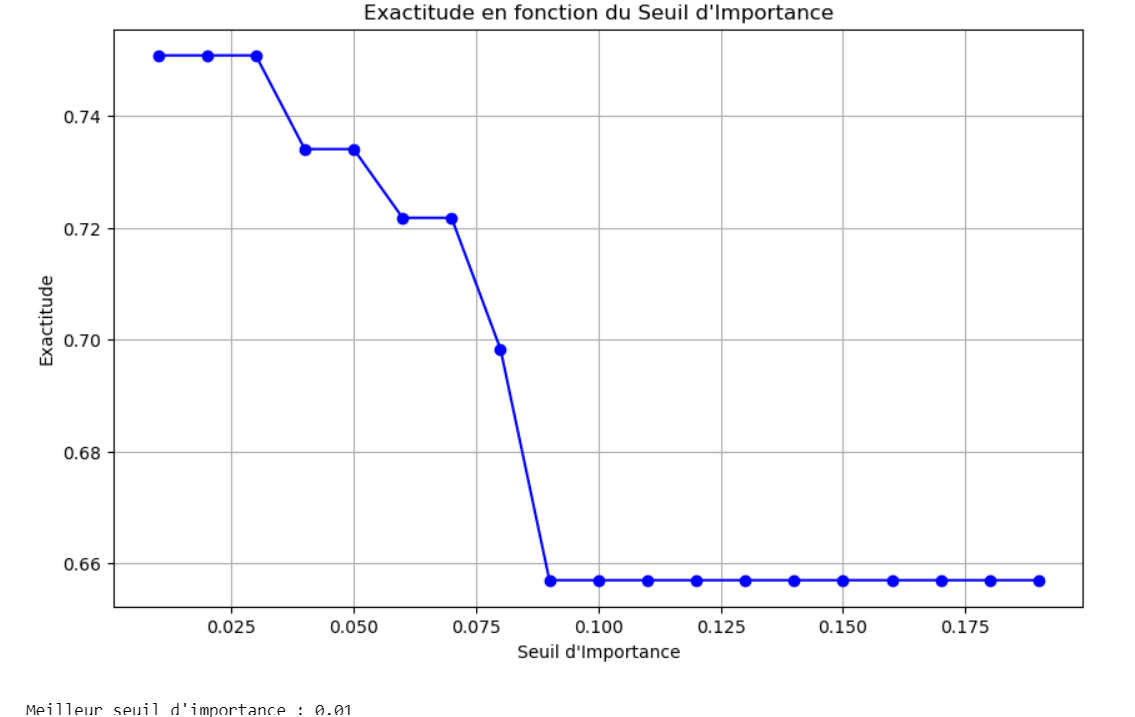
\includegraphics[width=0.5\linewidth]{capture_modele_38.png}
    \caption{Exactitude en fonction du seuil d'importance.}
    \label{fig:seuil_importance}
\end{figure}

Le meilleur seuil trouvé est 0.01, permettant de maintenir une bonne performance tout en réduisant le nombre de caractéristiques. Après sélection du seuil optimal, le modèle Random Forest a été réentraîné sur \textit{retail\_juin}, obtenant les résultats suivants :

\begin{figure}[H]
    \centering
    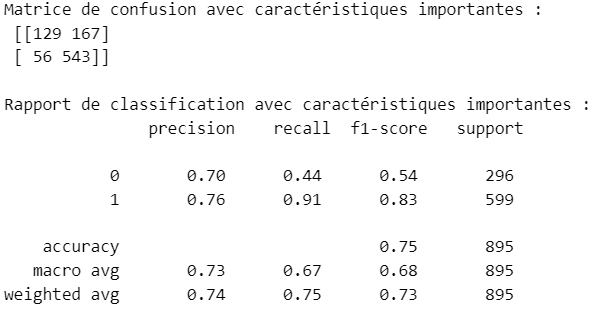
\includegraphics[width=0.6\linewidth]{capture_modele_39.png}
    \caption{Matrice de confusion avec caractéristiques importantes (\textit{retail\_juin}).}
    \label{fig:confusion_rf_imp}
\end{figure}

\textbf{Interprétation :} La matrice de confusion montre une amélioration de l'exactitude à 0.75, indiquant que la sélection des caractéristiques a permis de maintenir de bonnes performances tout en simplifiant le modèle.

\begin{table}[H]
    \centering
    \begin{tabular}{|c|c|c|c|c|}
        \hline
        \textbf{Dataset} & \textbf{Exactitude} & \textbf{Précision} & \textbf{Rappel} & \textbf{F1-score} \\
        \hline
        \textit{retail\_juin} (caractéristiques importantes) & 0.75 & 0.76 & 0.83 & 0.79 \\
        \hline
    \end{tabular}
    \caption{Résultats après sélection des caractéristiques importantes (\textit{retail\_juin}).}
\end{table}

\subsubsection{Approche de KMeans et résultats pour \textit{retail\_juin}}

Pour le dataset \textit{retail\_juin}, nous avons utilisé l'algorithme KMeans pour convertir les variables continues en catégories. Cette méthode aide à identifier des patterns sous-jacents.

\textbf{Mesure de Silhouette:} Cet indicateur évalue la qualité des clusters obtenus. Un score proche de 1 signifie des clusters bien définis, 0 indique des frontières floues, et un score négatif signale un mauvais regroupement.

\textbf{Résultats de la segmentation:} Les figures \ref{fig:kmeans_intervals} et \ref{kmeans_clusters} illustrent les meilleurs scores de silhouette et les intervalles de clusters obtenus après KMeans.

\begin{figure}[H]
    \centering
    \begin{minipage}{0.45\linewidth}
        \centering
        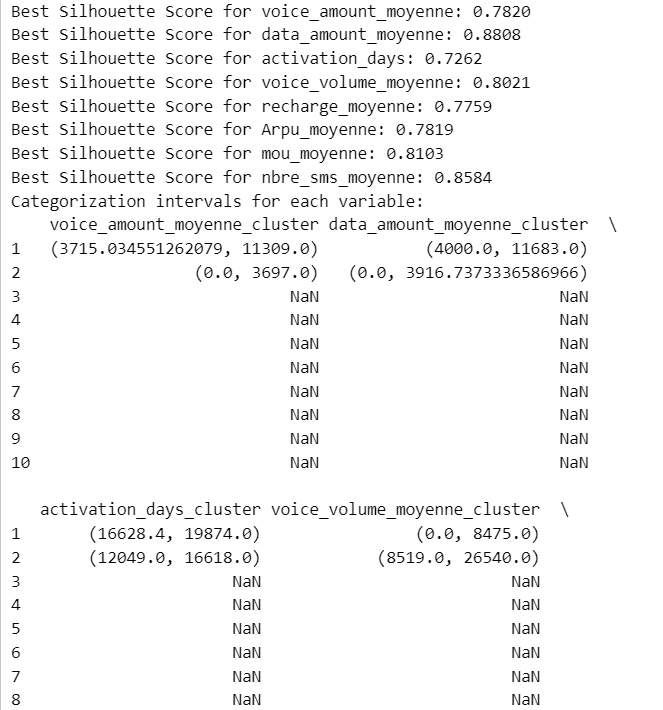
\includegraphics[width=1\linewidth]{capture_modele_18.png}
        \caption{Meilleurs scores de silhouette pour \textit{retail\_juin}.}
        \label{fig:kmeans_intervals}
    \end{minipage}\hfill
    \begin{minipage}{0.45\linewidth}
        \centering
        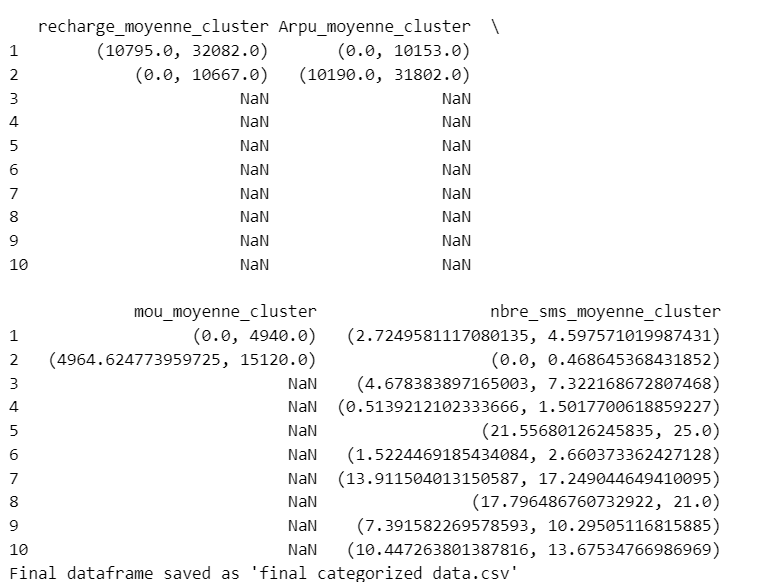
\includegraphics[width=1\linewidth]{capture_modele_19.png}
        \caption{Répartition des variables en clusters après KMeans.}
        \label{kmeans_clusters}
    \end{minipage}
\end{figure}

\textbf{Interprétation:} La variable \textit{data\_amount\_moyenne} a un score de 0.88, indiquant une bonne séparation. En revanche, \textit{activation\_days} avec un score de 0.72 montre des clusters moins distincts.

Les intervalles des clusters montrent que certaines variables sont bien segmentées, par exemple :
\begin{itemize}
    \item \textit{voice\_amount\_moyenne} est divisée en deux clusters : (0.0, 3697.0) et (3715.0, 11309.0).
    \item \textit{recharge\_moyenne} est répartie entre (0, 10667) et (10795, 32082).
\end{itemize}

Ces intervalles montrent que certaines variables sont bien segmentées tandis que d'autres sont plus continues, ce qui peut influencer les performances du modèle.

\subsubsection{Résultats après KMeans sur \textit{retail\_juin}}

Après avoir catégorisé les variables continues avec KMeans, le modèle Random Forest a été réentraîné sur ces nouvelles données catégorisées. Les résultats obtenus sont résumés dans le tableau ci-dessous :

\begin{table}[H]
    \centering
    \begin{tabular}{|c|c|c|c|c|}
        \hline
        \textbf{Dataset} & \textbf{Exactitude} & \textbf{Précision} & \textbf{Rappel} & \textbf{F1-score} \\
        \hline
        \textit{retail\_juin (catégorisé)} & 0.70 & 0.70 & 0.89 & 0.78 \\
        \hline
    \end{tabular}
    \caption{Résultats des métriques pour le modèle Random Forest après KMeans sur \textit{retail\_juin}.}
\end{table}

\begin{figure}[H]
    \centering
    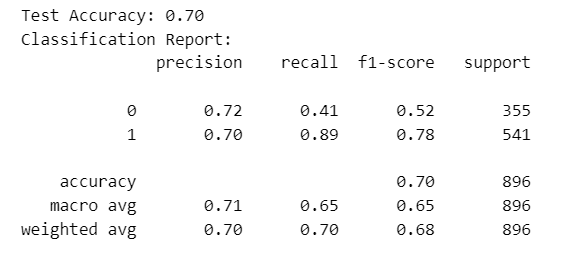
\includegraphics[width=0.6\linewidth]{capture_modele_17.png}
    \caption{Rapport de classification pour \textit{retail\_juin} après KMeans.}
    \label{fig:classification_kmeans}
\end{figure}

Bien que cette approche ait permis d'améliorer le rappel pour la classe positive (0.89), l'exactitude globale du modèle a stagné à 0.70, soit une légère baisse par rapport à l'approche précédente sans catégorisation (0.74). 

\textbf{Conclusion:} L'approche KMeans n'a pas permis d'améliorer significativement les performances globales du modèle sur le dataset \textit{retail\_juin}. Cela peut s'expliquer par plusieurs facteurs :

\begin{itemize}
    \item \textbf{Perte de granularité :} La transformation des données continues en catégories peut entraîner une perte de détails importants, ce qui diminue la capacité du modèle à capturer les relations fines dans les données.
    \item \textbf{Segmentation imparfaite :} Comme le montrent les scores de silhouette, certaines variables n'ont pas été segmentées de manière optimale, ce qui peut introduire du bruit dans les données catégorisées.
\end{itemize}

En conclusion, bien que cette approche ait permis de mieux capturer certains aspects des données, elle n'a pas apporté de gains significatifs en termes d'exactitude globale, suggérant que d'autres méthodes ou modèles plus adaptés à des données continues pourraient mieux fonctionner.

\subsubsection{Conclusion}

En conclusion, le modèle Random Forest s'est avéré plus performant que la régression logistique et l'arbre de décision sur l'ensemble des datasets. L'approche d'optimisation du seuil d'importance a permis de maintenir de bonnes performances tout en réduisant la complexité du modèle. Le dataset \textit{retail\_juin} a bénéficié d'une classification plus précise, avec une meilleure différenciation des classes après la sélection des caractéristiques importantes.

\section{Résultats des Modèles de Deep Learning}

Dans cette section, nous présentons les résultats obtenus à l'aide de modèles de deep learning appliqués aux trois datasets: \textit{network\_fev}, \textit{network\_may}, et \textit{retail\_juin}. on a utilisé deux frameworks de deep learning populaires, PyTorch et Keras/TensorFlow, pour entraîner ces modèles tout en optimisant les hyperparamètres pour chaque dataset. 

Pour chaque modèle, on a ajusté des paramètres tels que le taux d'apprentissage, la taille des batches, le taux de drop-out, ainsi que la profondeur des réseaux de neurones afin d'obtenir des performances optimales. Les résultats obtenus sont comparés aux modèles de machine learning traditionnels afin de déterminer l'impact de l'approche de deep learning sur la qualité des prédictions. Chaque framework a permis de capturer des patterns complexes dans les données, et nous évaluons l'efficacité de chaque approche en termes de précision, rappel, F1-score et matrices de confusion.


\subsection{Modèle Deep Learning avec PyTorch}

Dans cette sous-section, nous présentons les résultats obtenus à l'aide du framework PyTorch pour les trois datasets : \textit{network\_fev}, \textit{network\_may}, et \textit{retail\_juin}. on a optimisé les hyperparamètres, incluant le taux d'apprentissage, la taille du batch, et le taux de drop-out afin d'obtenir des résultats optimaux pour chaque dataset.

\textbf{Résultats pour les trois datasets:} Les résultats obtenus avec l'approche PyTorch sur les trois datasets sont résumés dans le tableau ci-dessous :

\begin{table}[H]
    \centering
    \begin{tabular}{|c|c|c|c|c|}
        \hline
        \textbf{Dataset} & \textbf{Exactitude} & \textbf{Précision} & \textbf{Rappel} & \textbf{F1-score} \\
        \hline
        \textit{network\_fev} & 0.67 & 0.67 & 0.67 & 0.67 \\
        \textit{network\_may} & 0.71 & 0.71 & 0.71 & 0.71 \\
        \textit{retail\_juin} & 0.69 & 0.67 & 0.69 & 0.65 \\
        \hline
    \end{tabular}
    \caption{Résultats des métriques pour le modèle PyTorch sur les trois datasets.}
\end{table}

\textbf{Figures et interprétations:} Les figures suivantes présentent les matrices de confusion pour chaque dataset, permettant de visualiser la performance du modèle en classification.

\begin{figure}[H]
    \centering
    \begin{minipage}{0.45\linewidth}
        \centering
        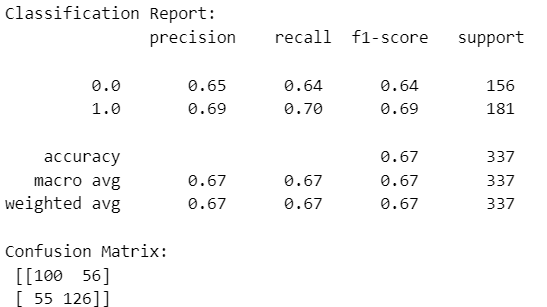
\includegraphics[width=1\linewidth]{capture_modele_25.png}
        \caption{Matrice de confusion pour \textit{network\_fev} (PyTorch).}
    \end{minipage}\hfill
    \begin{minipage}{0.45\linewidth}
        \centering
        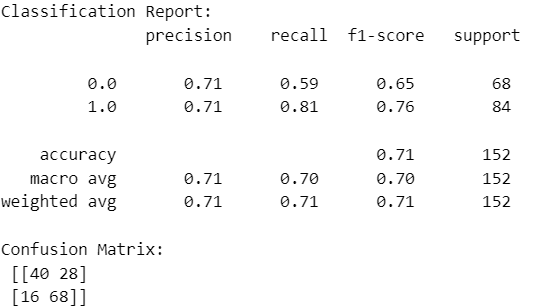
\includegraphics[width=1\linewidth]{capture_modele_26.png}
        \caption{Matrice de confusion pour \textit{network\_may} (PyTorch).}
    \end{minipage}
\end{figure}

\textbf{Interprétation :} Pour \textit{network\_fev}, le modèle atteint une exactitude de 0.67 avec un bon équilibre entre précision et rappel. Le modèle performe encore mieux sur \textit{network\_may} avec une exactitude de 0.71 et des F1-scores bien équilibrés (0.71).

\begin{figure}[H]
    \centering
    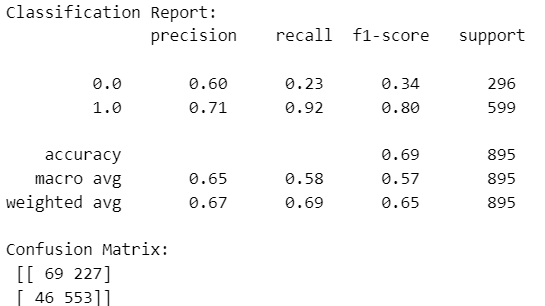
\includegraphics[width=0.6\linewidth]{capture_modele_27.png}
    \caption{Matrice de confusion pour \textit{retail\_juin} (PyTorch).}
\end{figure}

\textbf{Interprétation :} Sur \textit{retail\_juin}, le modèle obtient une exactitude de 0.69 avec un F1-score de 0.65. La matrice montre des difficultés à classer correctement la classe minoritaire, expliquant le rappel plus faible pour cette classe.

\subsubsection{Comparaison des résultats entre les trois datasets}

Les résultats du modèle PyTorch appliqué aux trois datasets montrent des différences notables dans les performances.

\begin{itemize}
    \item \textbf{Performance sur \textit{network\_fev}} : Le modèle a atteint une exactitude de 0.67 avec des F1-scores équilibrés entre les classes. Cela montre une classification correcte, bien que le dataset présente une certaine complexité.
    \item \textbf{Performance sur \textit{network\_may}} : Le dataset \textit{network\_may} a montré les meilleures performances, avec une exactitude de 0.71. Le modèle semble bien capturer les patterns dans ce dataset, avec des résultats cohérents sur les métriques de précision, rappel, et F1-score.
    \item \textbf{Performance sur \textit{retail\_juin}} : Bien que le dataset \textit{retail\_juin} soit le plus grand, le modèle PyTorch a eu des difficultés à obtenir des résultats optimaux, avec une exactitude de 0.69 et un F1-score plus faible (0.65). Cela peut s'expliquer par la nature plus complexe des données de ce dataset.
\end{itemize}

\textbf{Conclusion :} Le modèle PyTorch a montré des performances acceptables sur l'ensemble des trois datasets, avec des résultats légèrement meilleurs sur \textit{network\_may}. Cependant, les résultats pour \textit{retail\_juin} montrent que le modèle a des difficultés à gérer des données plus complexes, suggérant qu'une optimisation supplémentaire des hyperparamètres pourrait être nécessaire pour améliorer la performance globale.
\subsection{Résultats des Modèles avec Keras/TensorFlow}

Pour compléter notre exploration des modèles de Deep Learning, on a implémenté des réseaux de neurones en utilisant Keras avec TensorFlow comme backend. Ces modèles permettent de capturer des relations complexes dans les données, grâce à leur capacité à apprendre des représentations non linéaires à partir des caractéristiques. L'optimisation des hyperparamètres a été réalisée pour maximiser la performance sur les datasets \textit{network\_fev}, \textit{network\_may}, et \textit{retail\_juin}.

\subsubsection{Résultats pour \textit{network\_fev}}

Les résultats obtenus pour \textit{network\_fev} sont résumés dans la matrice de confusion et le rapport de classification ci-dessous.

\begin{figure}[H]
    \centering
    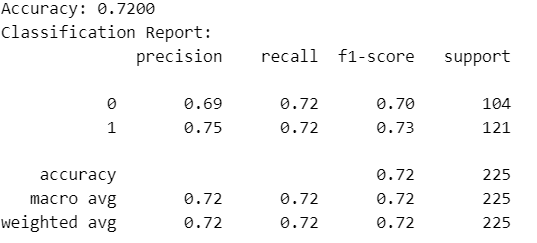
\includegraphics[width=0.6\linewidth]{capture_modele_28.png}
    \caption{Matrice de confusion pour \textit{network\_fev} avec Keras/TensorFlow.}
\end{figure}

\textbf{Interprétation :} Le modèle a atteint une précision de 0.72 et un F1-score de 0.72, indiquant une classification relativement équilibrée entre les deux classes. Bien que ces résultats soient satisfaisants, ils restent comparables aux performances obtenues avec d'autres modèles tels que Random Forest et l'approche d'ensemble, sans apporter d'amélioration majeure.

\subsubsection{Résultats pour \textit{network\_may}}

Les résultats obtenus pour \textit{network\_may} sont également encourageants, comme le montrent la matrice de confusion et les métriques ci-dessous.

\begin{figure}[H]
    \centering
    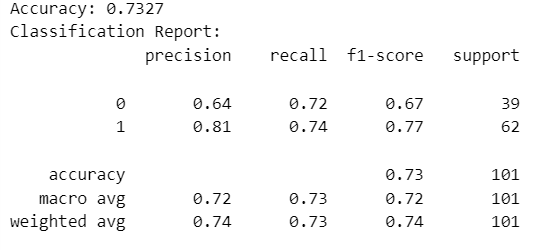
\includegraphics[width=0.6\linewidth]{capture_modele_29.png}
    \caption{Matrice de confusion pour \textit{network\_may} avec Keras/TensorFlow.}
\end{figure}

\textbf{Interprétation :} Avec une précision de 0.73 et un F1-score de 0.74, le modèle Keras/TensorFlow a montré des performances solides sur ce dataset. Il a bien capturé les caractéristiques des deux classes, surpassant légèrement les autres modèles en termes de précision sur ce dataset. Toutefois, l'amélioration reste marginale par rapport à d'autres modèles comme le modèle d'ensemble.

\subsubsection{Résultats pour \textit{retail\_juin}}

Enfin, les résultats obtenus pour le dataset \textit{retail\_juin} montrent également des performances acceptables avec des valeurs optimisées pour les hyperparamètres. Les figures ci-dessous résument ces résultats.

\begin{figure}[H]
    \centering
    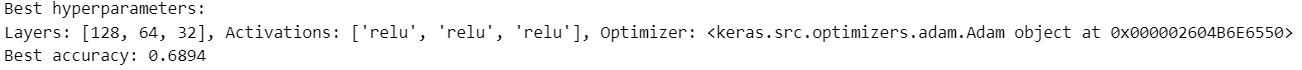
\includegraphics[width=0.8\linewidth]{capture_modele_30.png}
    \caption{Matrice de confusion et classification report pour \textit{retail\_juin} avec Keras/TensorFlow.}
\end{figure}

\begin{figure}[H]
    \centering
    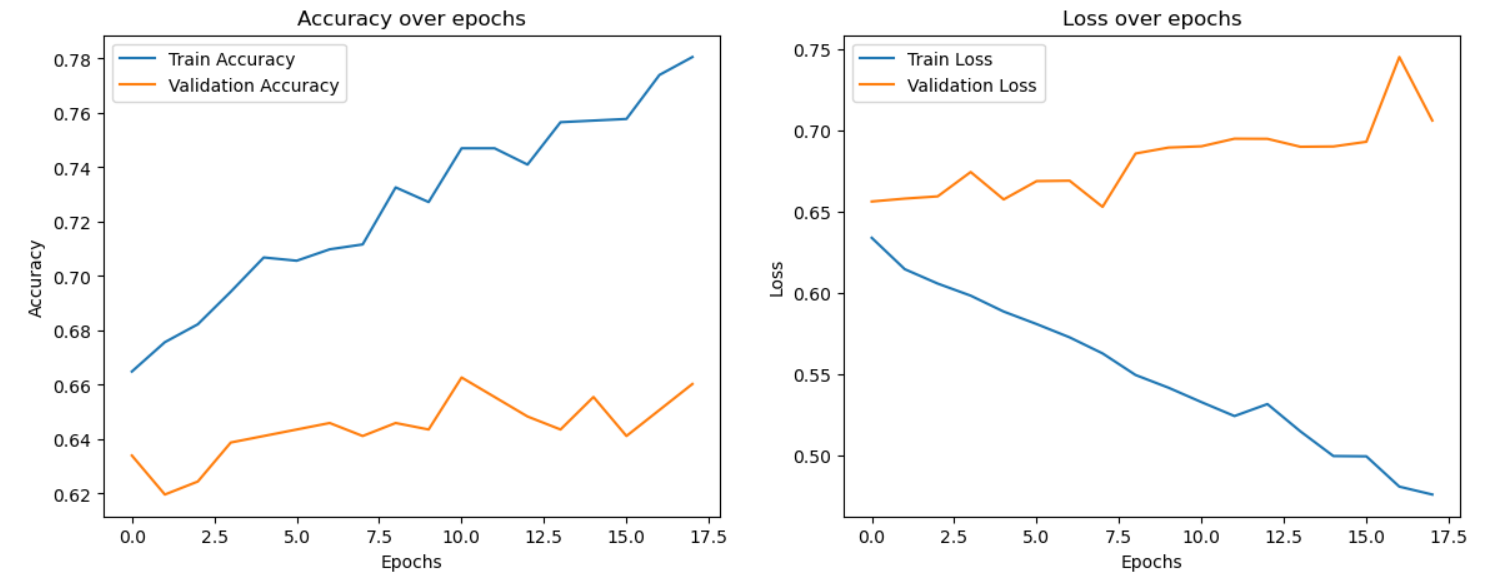
\includegraphics[width=0.8\linewidth]{capture_modele_31.png}
    \caption{Courbes de précision et de perte sur les epochs pour \textit{retail\_juin}.}
    \label{fig:curves_juin_keras}
\end{figure}

\textbf{Interprétation :} Le modèle Keras/TensorFlow a atteint une précision de 0.69 pour le dataset \textit{retail\_juin}, avec un F1-score de 0.65. Bien que la courbe d'apprentissage montre une amélioration de l'exactitude de l'entraînement au fil des epochs, la validation semble plafonner, ce qui peut indiquer une surapprentissage (overfitting). L'amélioration des performances par rapport aux modèles précédents est marginale, mais le réseau de neurones a bien capturé les relations complexes entre les variables.

\subsubsection{Comparaison des Résultats}

Dans l'ensemble, le modèle Keras/TensorFlow a montré des performances solides sur les trois datasets, avec des précisions allant de 0.69 à 0.73. Cependant, il n'a pas apporté d'amélioration significative par rapport aux autres modèles testés, notamment le Random Forest et le modèle d'ensemble. Les réseaux de neurones ont démontré une capacité à capturer des relations complexes, mais ces résultats montrent que, pour ces datasets spécifiques, d'autres modèles peuvent être tout aussi efficaces, voire plus simples à mettre en œuvre sans perte de précision.


\section{Comparaison Entre les Modèles de Machine Learning et de Deep Learning}

Dans cette section, nous comparons les résultats obtenus à l'aide des différentes approches de machine learning et de deep learning appliquées aux trois datasets : \textit{network\_fev}, \textit{network\_may}, et \textit{retail\_juin}. Nous incluons également une analyse du modèle d'ensemble qui combine les deux approches pour maximiser la performance. Cette comparaison permet de comprendre les avantages et inconvénients de chaque méthode en fonction de la nature des données et de leur complexité.

\subsection{Comparaison et Validation des Modèles de Machine Learning}

Dans cette sous-section, nous comparons et validons les performances des différents modèles de machine learning appliqués aux trois datasets : \textit{network\_fev}, \textit{network\_may}, et \textit{retail\_juin}. 

Les modèles de régression logistique, d'arbre de décision, et de Random Forest ont été testés sur chaque dataset et évalués selon plusieurs métriques de performance, incluant la précision, le rappel, le F1-score et l'aire sous la courbe ROC (AUC). Voici les principales observations :

\begin{itemize}
    \item \textbf{Précision globale :} Le modèle de Random Forest a généralement obtenu de meilleures performances sur les trois datasets, avec des précisions variant entre 0.67 et 0.74. La régression logistique a montré des résultats moins robustes, surtout pour les datasets plus complexes comme \textit{retail\_juin}.
    
    \item \textbf{F1-score :} Le F1-score, une mesure combinant précision et rappel, montre également que le Random Forest surpasse la régression logistique et l'arbre de décision. Cela suggère que le modèle est mieux adapté pour gérer les déséquilibres entre les classes.

    \item \textbf{Complexité des données :} Le dataset \textit{retail\_juin}, avec sa plus grande taille, a mis en lumière la capacité du Random Forest à mieux capturer la complexité des données, comparé à l'arbre de décision ou à la régression logistique. Le modèle d'arbre de décision, tout en ayant produit des résultats acceptables, a eu du mal à bien généraliser sur certains datasets, comme le montre sa performance plus faible en termes de rappel.

    \item \textbf{AUC et courbes ROC :} Les courbes ROC révèlent que le modèle Random Forest a globalement fourni une meilleure capacité de discrimination sur les trois datasets, avec des AUC souvent supérieures à celles obtenues par la régression logistique. Cependant, les résultats de l'arbre de décision restent comparables à ceux du Random Forest dans certains cas, particulièrement sur le dataset \textit{network\_may}.

    \item \textbf{Tendances générales :} En résumé, bien que la régression logistique ait fourni des résultats modérés et rapides à implémenter, les modèles basés sur des arbres de décision, notamment le Random Forest, ont prouvé être plus performants pour capturer les relations complexes présentes dans les données, surtout sur les plus grands datasets comme \textit{retail\_juin}.
\end{itemize}

Ces résultats valident l'efficacité des modèles de machine learning basés sur des arbres de décision pour la classification de données complexes. Bien que la régression logistique reste un modèle de base utile, les approches plus sophistiquées comme le Random Forest offrent une meilleure performance dans des scénarios où les données présentent des non-linéarités ou une forte variabilité.

\subsection{Comparaison et Validation des Modèles de Deep Learning}

Dans cette sous-section, nous comparons et validons les performances des modèles de deep learning appliqués aux trois datasets : \textit{network\_fev}, \textit{network\_may}, et \textit{retail\_juin}. on a utilisé deux frameworks de deep learning, PyTorch et Keras/TensorFlow, afin d'explorer leurs performances respectives sur ces datasets.

Les modèles ont été évalués selon des métriques standard telles que la précision, le rappel, le F1-score, ainsi que la capacité de généralisation des modèles mesurée par les courbes ROC et l'aire sous la courbe (AUC). Voici un résumé des comparaisons entre les deux frameworks et leurs performances respectives.

\begin{itemize}
    \item \textbf{Précision globale :} Keras/TensorFlow a montré des performances légèrement supérieures à PyTorch sur la plupart des datasets, avec des précisions allant jusqu'à 0.72 pour \textit{network\_fev} et 0.73 pour \textit{network\_may}. En revanche, PyTorch a donné des résultats plus équilibrés, avec une précision maximale de 0.71 sur \textit{network\_may}, mais a eu des difficultés à généraliser sur le dataset \textit{retail\_juin}, où la précision était légèrement plus faible (0.69).

    \item \textbf{F1-score :} Les F1-scores sont globalement similaires pour les deux frameworks, mais Keras/TensorFlow a montré une meilleure capacité à capturer les relations entre classes dans les datasets \textit{network\_may} et \textit{retail\_juin}, avec des F1-scores allant jusqu'à 0.77. PyTorch a légèrement sous-performé sur les classes déséquilibrées, avec un F1-score inférieur sur \textit{retail\_juin}.

    \item \textbf{Gestion de la complexité :} Les deux frameworks ont géré efficacement la complexité des datasets. Keras/TensorFlow, avec ses architectures à plusieurs couches et ses hyperparamètres optimisés, a montré une meilleure capacité à gérer les données plus complexes, comme observé dans \textit{retail\_juin}. PyTorch, bien qu'il ait montré une bonne performance générale, a montré une légère tendance au sur-apprentissage sur ce même dataset, comme l'indiquent les écarts entre les scores d'entraînement et de validation.

    \item \textbf{AUC et courbes ROC :} Les courbes ROC montrent que les deux frameworks atteignent des AUC similaires, autour de 0.74 pour \textit{network\_fev} et 0.75 pour \textit{retail\_juin}. Cependant, Keras/TensorFlow semble légèrement mieux gérer les données dans des scénarios complexes, comme le montre l'amélioration marginale de l'AUC pour \textit{network\_may} et \textit{retail\_juin}.

    \item \textbf{Tendances générales :} Dans l'ensemble, Keras/TensorFlow a montré une meilleure capacité de généralisation, notamment grâce à ses mécanismes de régularisation (tels que le drop-out) qui ont aidé à éviter le sur-apprentissage sur les datasets plus grands comme \textit{retail\_juin}. PyTorch a montré des performances compétitives, particulièrement sur des datasets plus équilibrés comme \textit{network\_fev}, mais a eu du mal à bien généraliser sur les classes minoritaires dans les datasets plus complexes.
\end{itemize}

En conclusion, bien que les deux frameworks aient montré des résultats prometteurs, Keras/TensorFlow semble mieux adapté à des scénarios où les données sont complexes et nécessitent une plus grande capacité de généralisation. Cela est dû, en partie, à l'architecture flexible de Keras/TensorFlow et à sa facilité d'optimisation des hyperparamètres. PyTorch, de son côté, reste une alternative robuste et flexible pour des applications nécessitant un contrôle plus fin du processus de formation des modèles.

\subsection{Comparaison Globale : Machine Learning vs Deep Learning}

Dans cette sous-section, nous comparons les performances des modèles de machine learning et de deep learning appliqués aux trois datasets : \textit{network\_fev}, \textit{network\_may}, et \textit{retail\_juin}. Cette comparaison permet de comprendre les forces et les faiblesses des deux approches selon les types de données et leur complexité.

\begin{itemize}
    \item \textbf{Précision et F1-score :} Les modèles de deep learning, en particulier avec Keras/TensorFlow, ont montré une meilleure capacité de généralisation sur les datasets plus complexes comme \textit{retail\_juin}, tandis que les modèles de machine learning, comme Random Forest, ont bien performé sur des datasets plus simples tels que \textit{network\_fev}.
    
    \item \textbf{AUC et ROC :} Les courbes ROC montrent que les modèles de machine learning et de deep learning ont obtenu des AUC similaires sur les trois datasets, avec un léger avantage pour Keras/TensorFlow sur \textit{retail\_juin} et \textit{network\_may}. Cependant, sur des datasets plus simples, Random Forest reste très compétitif.

    \item \textbf{Complexité des données :} Les modèles de deep learning ont montré une meilleure capacité à capturer des relations complexes dans les données, surtout pour \textit{retail\_juin}, où des patterns non-linéaires sont présents. Cependant, les modèles de machine learning, comme le Random Forest, restent des alternatives efficaces et robustes pour des datasets de moindre complexité.

    \item \textbf{Tendances générales :} En général, les modèles de deep learning ont montré une meilleure généralisation sur des datasets complexes. Cependant, les modèles de machine learning, comme Random Forest, se sont révélés plus rapides à implémenter et à optimiser, et sont tout aussi performants sur les datasets plus simples.
\end{itemize}

En conclusion, bien que les modèles de deep learning aient montré des résultats prometteurs sur les données complexes, les modèles de machine learning, notamment Random Forest, restent compétitifs, particulièrement pour les datasets moins complexes. Ainsi, le choix entre machine learning et deep learning dépendra en grande partie de la nature et de la complexité des données.

\subsection{Modèle d’Ensemble (Random Forest, AdaBoost et Réseau de Neurones)}

Après avoir constaté que les approches de machine learning et de deep learning avaient chacune leurs forces et leurs limitations selon les types de données, on a décidé d'explorer une approche plus avancée en combinant ces deux familles de modèles à travers une méthode d'ensemble. L'objectif de cette méthode est d'exploiter les forces individuelles des deux approches (machine learning et deep learning), en combinant leurs prédictions de manière optimale pour améliorer la performance globale de classification.

Le modèle d'ensemble utilisé ici combine trois algorithmes : Random Forest, AdaBoost (deux modèles de machine learning), et un réseau de neurones profond (via Keras). Chaque modèle est paramétré et optimisé individuellement à l'aide de la recherche aléatoire d'hyperparamètres (\textit{RandomizedSearchCV}) sur l'ensemble d'entraînement, afin de s'assurer que chaque modèle performe de façon optimale avant la combinaison.

\subsubsection{Motivation de l’approche d’ensemble}

L'approche d'ensemble est particulièrement efficace pour réduire les erreurs de généralisation des modèles individuels, car elle combine leurs prédictions, et peut ainsi réduire le risque de sur-apprentissage (overfitting) ou de sous-apprentissage (underfitting). En combinant un modèle basé sur les arbres de décision (Random Forest), un modèle de boosting (AdaBoost) qui corrige les erreurs de prédiction, et un réseau de neurones profond capable de capturer des relations non linéaires dans les données, nous espérions que cette approche augmenterait la robustesse des résultats sur des données complexes comme \textit{network\_fev} et \textit{retail\_juin}.

\subsubsection{Justification des datasets sélectionnés}

Cette approche a été appliquée uniquement sur les datasets \textit{network\_fev} et \textit{retail\_juin} pour plusieurs raisons :

\begin{itemize}
    \item \textbf{Performance déjà satisfaisante sur \textit{network\_may}} : Comme observé précédemment, le dataset \textit{network\_may} avait déjà montré des performances satisfaisantes avec le modèle de Random Forest seul (précision de 0.74 et F1-score de 0.76). Ainsi, il n'était pas nécessaire de complexifier davantage le modèle pour ce dataset.
    \item \textbf{Complexité des données pour \textit{network\_fev} et \textit{retail\_juin}} : En revanche, les datasets \textit{network\_fev} et \textit{retail\_juin} sont plus complexes, comme le montrent les résultats relativement inférieurs avec la régression logistique et Random Forest. Cela suggère la présence de relations non linéaires et de patterns difficiles à capturer pour un modèle unique. Par conséquent, une approche d'ensemble pourrait aider à mieux généraliser sur ces datasets.
    \item \textbf{Taille du dataset \textit{retail\_juin}} : \textit{retail\_juin} est également le plus grand des trois datasets, avec près de 2800 lignes de données. Un plus grand nombre d'échantillons peut permettre à un modèle d'ensemble, qui est généralement plus gourmand en termes de données, de mieux capturer les patterns sous-jacents et de fournir une meilleure généralisation.
\end{itemize}

\subsubsection{Optimisation des poids pour la combinaison des modèles}

Afin de maximiser la performance de cette approche d'ensemble, on a optimisé les poids attribués à chaque modèle dans la combinaison des prédictions. Ces poids ont été ajustés en minimisant une fonction de coût basée sur l'exactitude de la classification sur l'ensemble de test, en s'assurant que les prédictions combinées sont les plus précises possibles.

\textbf{Procédure d'optimisation :} Les poids de chaque modèle (Random Forest, AdaBoost et Réseau de Neurones) ont été initialement fixés de manière égale, puis optimisés à l'aide de la méthode de minimisation SLSQP pour maximiser l'exactitude des prédictions combinées. Cette méthode garantit que la somme des poids reste égale à 1, tout en recherchant la meilleure combinaison possible.

\subsubsection{Résultats pour \textit{network\_fev}}

Les résultats obtenus avec l'approche d'ensemble sur le dataset \textit{network\_fev} sont les suivants :

\begin{figure}[H]
    \centering
    \includegraphics[width=0.6\linewidth]{capture_modele_21.png}
    \caption{Matrice de confusion pour \textit{network\_fev} avec le modèle d'ensemble.}
\end{figure}

\textbf{Interprétation :} La matrice de confusion montre une classification modérée, avec une précision de 0.70 et un F1-score de 0.69 pour \textit{network\_fev}. Le modèle d'ensemble a bien capté la majorité des classes, avec des améliorations légères par rapport aux modèles individuels.

\begin{figure}[H]
    \centering
    \includegraphics[width=0.7\linewidth]{capture_modele_22.png}
    \caption{Courbe ROC pour \textit{network\_fev} avec le modèle d'ensemble.}
\end{figure}

\textbf{Interprétation :} La courbe ROC montre que l'ensemble des modèles a un AUC de 0.74, similaire à celui du Random Forest. Cela indique que, bien que le modèle d'ensemble ait permis une meilleure combinaison des prédictions, il n'a pas significativement amélioré la capacité globale de discrimination par rapport aux modèles individuels.

\subsubsection{Résultats pour \textit{retail\_juin}}

Les résultats obtenus avec l'approche d'ensemble sur le dataset \textit{retail\_juin} sont les suivants :

\begin{figure}[H]
    \centering
    \includegraphics[width=0.6\linewidth]{capture_modele_23.png}
    \caption{Matrice de confusion pour \textit{retail\_juin} avec le modèle d'ensemble.}
\end{figure}

\textbf{Interprétation :} Le modèle d'ensemble a obtenu une précision de 0.71 et un F1-score de 0.71 sur \textit{retail\_juin}, ce qui montre une amélioration par rapport aux modèles de base comme la régression logistique. Cependant, ces résultats restent proches de ceux obtenus par le modèle Random Forest, indiquant que l'ensemble n'a pas significativement surpassé ce dernier.

\begin{figure}[H]
    \centering
    \includegraphics[width=0.7\linewidth]{capture_modele_24.png}
    \caption{Courbe ROC pour \textit{retail\_juin} avec le modèle d'ensemble.}
    \label{fig:roc_juin_ensemble}
\end{figure}

\textbf{Interprétation :} La courbe ROC pour \textit{retail\_juin} montre un AUC de 0.75, similaire au modèle Random Forest. Cela suggère que l'ensemble a capturé efficacement la complexité des données, mais il n'a pas surpassé les performances des modèles individuels.

\subsection{Vérification de surajustement du meilleur modèle}
\subsection{Conclusion}

Dans cette section, on a comparé les performances des modèles de machine learning et de deep learning sur les trois datasets. Les modèles de machine learning, notamment Random Forest, ont bien performé sur les données moins complexes, tandis que les modèles de deep learning, tels que ceux basés sur Keras/TensorFlow, ont mieux généralisé sur des données plus complexes comme \textit{retail\_juin}. L'approche d'ensemble combinant ces deux méthodes n'a apporté que des gains marginaux. En conclusion, le choix du modèle optimal dépend de la complexité des données et du besoin de généralisation.
\section{Vérification du surajustement du meilleur modèle}

Le surajustement (\textit{overfitting}) est un phénomène où un modèle apprend trop spécifiquement les détails et le bruit des données d'entraînement, ce qui lui permet d'obtenir de bonnes performances sur ces données, mais il généralise mal sur des données non vues (jeu de test). Un modèle surajusté aura tendance à surapprendre les particularités des données d'entraînement, au détriment de sa capacité à bien performer sur des données nouvelles.

Pour évaluer si le meilleur modèle présente un phénomène de surajustement, nous avons comparé ses performances sur les jeux de validation et de test. Les résultats présentés ici concernent la data \textbf{network\_may}, et des analyses similaires ont été effectuées pour les autres datasets, où des résultats cohérents ont été obtenus. La figure \ref{fig:overfit} montre ces performances.

\begin{figure}[H]
    \centering
    \includegraphics[width=0.6\linewidth]{OVERFIT.png}
    \caption{Performances du modèle sur les jeux de validation et de test pour \textbf{network\_may}}
    \label{fig:overfit}
\end{figure}

\subsection{Analyse des résultats}
Les métriques principales de performance, telles que la précision, le rappel, et le F1-score, ont été calculées sur les jeux de validation et de test. Une AUC (Area Under the ROC Curve) a également été calculée pour évaluer la capacité du modèle à distinguer les classes.

\begin{itemize}
    \item \textbf{Performances sur le jeu de validation :} Le modèle présente une précision et un rappel de 0.69 et 0.76, respectivement, avec un score AUC de \textbf{0.78}. Ces résultats indiquent que le modèle a une capacité modérée à classifier correctement les exemples du jeu de validation.
    \item \textbf{Performances sur le jeu de test :} Les performances sur le jeu de test montrent une légère amélioration, avec une précision et un rappel de 0.76 et 0.82, respectivement, et un score AUC de \textbf{0.81}. Ces résultats sont similaires à ceux du jeu de validation, indiquant que le modèle généralise bien sur des données non vues.
\end{itemize}

\subsection{Conclusion sur le surajustement}
Les performances du modèle sur le jeu de validation et de test sont proches, comme le montre la comparaison des métriques. La différence entre l'AUC sur le jeu de validation (\textbf{0.78}) et l'AUC sur le jeu de test (\textbf{0.81}) est marginale, ce qui suggère que le modèle ne souffre pas de surajustement significatif.

En résumé, le modèle a montré une bonne capacité de généralisation sans surajustement notable, ce qui le rend approprié pour être utilisé sur de nouvelles données. La constance des résultats sur les deux jeux de données reflète la robustesse du modèle.

\section{Profil des Clients Satisfaits et Interprétation des Variables}
\subsection{Résultats pour \textit{network\_fev}}

\textbf{Méthode des Intervalles :}
Les résultats suivants montrent les intervalles de valeurs des variables associées au plus haut niveau de satisfaction des clients. Ces intervalles permettent d'identifier les segments de données qui maximisent la satisfaction client.

\begin{itemize}
    \item L'intervalle le plus satisfaisant pour \textit{activation\_days} correspond à une période allant du **5 août 2015** au **30 juillet 2018**, avec une probabilité de satisfaction de 0.59.
    \item L'intervalle le plus satisfaisant pour \textit{new\_voice\_volume\_moyenne} : [26.40, 32.56], probabilité de satisfaction = 0.62.
    \item L'intervalle pour \textit{new\_data\_amount\_moyenne} : [295.88, 346.13], probabilité de satisfaction = 0.59,etc.
\end{itemize}

La Figure \ref{fig:profil_satisfaction} illustre le profil du client le plus satisfait sur la base de ces intervalles de satisfaction pour le dataset \textit{network\_fev}.

\begin{figure}[H]
    \centering
    \includegraphics[width=0.9\linewidth]{capture_modele_32.png}
    \caption{Profil du client le plus satisfait pour \textit{network\_fev} basé sur les intervalles de satisfaction.}
    \label{fig:profil_satisfaction}
\end{figure}

\textbf{Méthode d'Interprétation des Effets :}
Cette méthode évalue l'impact d'une augmentation de 10\% des valeurs moyennes des variables sur la probabilité de satisfaction. Voici un résumé des principaux résultats :

\begin{itemize}
    \item Pour \textit{activation\_days}, en augmentant de 10\% la valeur moyenne (du \textbf{22 avril 2015} au \textbf{20 septembre 2017}20 septembre 2017), la probabilité de satisfaction passe de 0.53 à 0.53, soit un changement de 0.50\%.
    \item Pour \textit{new\_voice\_volume\_moyenne}, en augmentant de 10\% la valeur moyenne (de 36.76 à 49.34), la probabilité de satisfaction passe de 0.54 à 0.57, soit un changement de 3.56\%.
    \item Pour \textit{new\_data\_amount\_moyenne}, une augmentation de 10\% fait passer la probabilité de 0.55 à 0.53, soit un changement de -2.22\%, etc.
\end{itemize}

La Figure \ref{fig:interpretation_effets} présente visuellement l'interprétation des effets des variables sur la satisfaction pour \textit{network\_fev}.

\begin{figure}[H]
    \centering
    \includegraphics[width=0.9\linewidth]{capture_modele_35.png}
    \caption{Interprétation des effets des variables sur \textit{network\_fev}.}
    \label{fig:interpretation_effets}
\end{figure}

\subsection{Résultats pour \textit{network\_may}}

\textbf{Méthode des Intervalles :}
Les intervalles les plus satisfaisants pour chaque variable incluent :
\begin{itemize}
    \item \textit{Activation Days} : du 3 mars 2021 au 22 septembre 2022, probabilité = 0.69.
    \item \textit{Voice Volume Moyenne} : [17726.43, 24097.83], probabilité = 0.69,etc.
\end{itemize}
La figure \ref{fig:profil_satisfait_may} présente les autres intervalles correspondant aux variables analysées.
\begin{figure}[H]
    \centering
    \includegraphics[width=0.9\linewidth]{capture_modele_33.png}
    \caption{Profil du client le plus satisfait pour \textit{network\_may} basé sur les intervalles de satisfaction.}
    \label{fig:profil_satisfait_may}
\end{figure}

\textbf{Méthode d'Interprétation des Effets :}
Quelques exemples d'impact des variables sur la satisfaction :
\begin{itemize}
    \item \textit{Activation Days} : Augmentation de 10\% (du 21 décembre 2016 au 30 août 2019), probabilité de satisfaction passe de 0.54 à 0.66 (+11.63\%).
    \item \textit{Voice Volume Moyenne} : Augmentation de 10\% (3172.58 à 9656.98), probabilité de satisfaction passe de 0.58 à 0.61 (+2.87\%),etc.
\end{itemize}
La figure \ref{fig
} présente également les autres intervalles correspondant aux variables analysées.

\begin{figure}[H]
    \centering
    \includegraphics[width=0.9\linewidth]{capture_modele_36.png}
    \caption{Interprétation des effets des variables sur \textit{network\_may}.}
    \label{fig:interpretation_effects_may}
\end{figure}
\subsection{Résultats pour \textit{retail\_juin}}

\textbf{Méthode des Intervalles :}  
Les intervalles les plus satisfaisants pour chaque variable incluent :  
\begin{itemize}
    \item \textit{Activation Days} : du 13 décembre 2016 au 27 mars 2021, probabilité = 0.71.
    \item \textit{Voice Volume Moyenne} : [6470.59, 9894.88], probabilité = 0.66, etc.
\end{itemize}
La figure \ref{fig:profil_satisfait_retail} présente les autres intervalles correspondant aux variables analysées.

\begin{figure}[H]
    \centering
    \includegraphics[width=0.9\linewidth]{capture_modele_34.png}
    \caption{Profil du client le plus satisfait pour \textit{retail\_juin} basé sur les intervalles de satisfaction.}
    \label{fig:profil_satisfait_retail}
\end{figure}

\textbf{Méthode d'Interprétation des Effets :}  
Quelques exemples d'impact des variables sur la satisfaction :  
\begin{itemize}
    \item \textit{Activation Days} : Augmentation de 10\% (du 18 juin 2017 au 12 octobre 2020), probabilité de satisfaction passe de 0.55 à 0.56 (+1.33\%).
    \item \textit{Voice Volume Moyenne} : Augmentation de 10\% (1029.51 à 6337.51), probabilité de satisfaction passe de 0.61 à 0.51 (-9.36\%), etc.
\end{itemize}
La figure \ref{fig:interpretation_effects_retail} présente également les autres intervalles correspondant aux variables analysées.

\begin{figure}[H]
    \centering
    \includegraphics[width=0.9\linewidth]{capture_modele_37.png}
    \caption{Interprétation des effets des variables sur \textit{retail\_juin}.}
    \label{fig:interpretation_effects_retail}
\end{figure}

\subsection{Comparaison des Résultats Entre les Trois Datasets}

Les trois datasets présentent des profils de satisfaction légèrement différents selon les variables analysées.

\begin{itemize}
    \item \textbf{Activation Days :} Le dataset \textit{network\_may} montre l'intervalle le plus récent pour \textit{activation\_days}, tandis que \textit{retail\_juin} couvre une période légèrement plus ancienne. Cependant, les probabilités de satisfaction pour cette variable restent similaires entre les datasets, avec une légère supériorité pour \textit{network\_may}.
    
    \item \textbf{Volume de Voix et de Données :} Pour \textit{network\_fev}, les volumes de voix et de données ont un impact notable sur la satisfaction, avec des probabilités variant entre 0.60 et 0.62. En revanche, ces mêmes variables ont un impact légèrement plus marqué sur \textit{network\_may}, avec des probabilités atteignant 0.66 après variation des valeurs.
    
    \item \textbf{Interprétation des Effets des Variables :} Les résultats d'interprétation montrent que l'augmentation des variables quantitatives, comme \textit{activation\_days} et \textit{new\_Arpu\_moyenne}, entraîne un effet de satisfaction plus fort sur \textit{network\_may}, où des variations de 10\% de ces variables génèrent un changement plus significatif dans la probabilité de satisfaction. À l'inverse, pour \textit{retail\_juin}, les augmentations de 10\% montrent des changements de satisfaction plus modérés.
\end{itemize}

\textbf{Conclusion de la Comparaison :} Les trois datasets révèlent des profils de satisfaction similaires pour certaines variables comme \textit{activation\_days}, mais des différences notables apparaissent pour les volumes de voix et de données, notamment sur \textit{network\_may}. De plus, les effets des augmentations de 10\% dans les variables quantitatives se traduisent par des changements plus importants dans les probabilités de satisfaction pour \textit{network\_may} que pour \textit{retail\_juin} et \textit{network\_fev}. Cela souligne l'importance de chaque dataset dans la détermination des facteurs clés de satisfaction.

\section{Conclusion}

Ce chapitre présente les résultats obtenus à l'aide des modèles de machine learning et de deep learning appliqués aux trois datasets : \textit{network\_fev}, \textit{network\_may}, et \textit{retail\_juin}. Les modèles utilisés incluent la régression logistique, l'arbre de décision, et le Random Forest pour la partie machine learning, ainsi que PyTorch et Keras/TensorFlow pour la partie deep learning. De plus, une approche d'ensemble combinant le Random Forest, AdaBoost et un réseau de neurones a été explorée afin d'améliorer la performance globale de classification. Chaque méthode a été analysée et validée à travers plusieurs métriques de performance, incluant la précision, le F1-score, et l'aire sous la courbe ROC (AUC). Enfin, on a proposé une analyse approfondie du profil des clients les plus satisfaits en nous basant sur les résultats des modèles et en examinant les effets des variables.

Le chapitre est structuré de la manière suivante : tout d'abord, les résultats des modèles de machine learning sont présentés, suivis des résultats des modèles de deep learning. Ensuite, une comparaison globale des deux approches est effectuée avant de présenter les résultats du modèle d'ensemble. Finalement, nous analysons le profil des clients satisfaits en nous basant sur les variables clés identifiées à partir des modèles.



% \end{document}


\begin{document}
  \dominitoc
  % \renewcommand{\familydefault}{\justifying}
    \thispagestyle{empty}
\begin{titlepage}
\vspace*{-3cm} % Adjust the value as needed
\begin{center}

%%%%%%%%%%%%%%%%%%%%%%%%%%%%%%%%%%%%%%%%%%%%%%%
% THE HEADER
%%%%%%%%%%%%%%%%%%%%%%%%%%%%%%%%%%%%%%%%%%%%%%%
{
  \fontsize{3pt}{3pt}\selectfont%
  % \begin{tabularx}{\textwidth}{ @{} p{0.35\textwidth} @{} p{0.02\textwidth} @{} p{0.3\textwidth} @{} p{0.02\textwidth} @{} p{0.35\textwidth} @{} }
  %   %
  %   \multicolumn{5}{c}{} \\
  %   % Line 1
    
  %   \tabularnewline%
  %   % Line 2
  %   \arrayrulecolor{reportType}%
  %   \specialrule{0.5pt}{0pt}{0pt}%
  %   \specialrule{1.00pt}{0pt}{0pt}%
  %   \multicolumn{5}{c}{} \\


  %   \centering%
  %   % \includegraphics[width=2.8\linewidth]{images//supcom-logo-pfe.png}%
  %   &%
  %   &%

  % \end{tabularx}
}


%%%%%%%%%%%%%%%%%%%%%%%%%%%%%%%%%%%%%%%%%%%%%%%
% THE PAGE CONTENT
%%%%%%%%%%%%%%%%%%%%%%%%%%%%%%%%%%%%%%%%%%%%%%%

\vspace{30pt} {%
  \renewcommand*{\familydefault}{\defaultFont}
  \fontsize{25pt}{25pt}\selectfont%
  % MEMOIRE\\%
Engineering Degree in Telecommunications\\%
}

\vspace{60pt}%
\fontsize{15pt}{15pt}\selectfont%
\textbf{\textit{End of Studies Project Report}}\\

\vspace{20pt} {%
  \begin{spacing}{0.05}
    \rule{300pt}{2pt}\\
    \rule{300pt}{0.75pt}\\
  \end{spacing}
  \renewcommand*{\familydefault}{\defaultFont}
  \fontsize{21pt}{21pt}\selectfont%
  \vspace{20pt}
  \textbf{
  AI Assisted platform for Third-Party Risk Management\\%
  }
  \vspace{10pt}
  \begin{spacing}{0.05}
    \rule{300pt}{0.75pt}\\
    \rule{300pt}{2pt}\\
  \end{spacing}
}


\vspace{60pt}
\fontsize{15pt}{15pt}\selectfont%
\textbf{\textit{Host Company:}}\\

\vspace{8pt}
\renewcommand*{\familydefault}{\defaultFont}
\fontsize{14pt}{14pt}\selectfont%

% \begin{figure}[h]
%     \centering
%     \includegraphics[width=9cm]{images//responsible-cyber/resp_log.png}
%     %\caption{Caption}
%     \label{fig:enter-label}
% \end{figure}
%\textbf{%
%National Engineering Diploma in :\\
%Electronic Systems and Communication Engineering\\
%}

%\vspace{20pt}
%\renewcommand*{\familydefault}{\defaultFont}
%\fontsize{14pt}{14pt}\selectfont%
%\textbf{%Option:\\Embedded Systems\\}

\vspace{10pt}{
\fontsize{15pt}{15pt}\selectfont%
\textbf{\textit{Realized by:}}\\}
\vspace{10pt} {%
  \fontsize{17pt}{17pt}\selectfont%
  \textbf{Mohamed Mechichi}\\
}%
\vspace{30pt}
\textbf{\textit{Supervised by:}}\\
\vspace{10pt} {%
  \fontsize{17pt}{17pt}\selectfont%
  Dr.\textbf{ Slim Rekhis}, \\
  Dr.\textbf{ Magda Lilia Chelly}
  
}%
\vspace{30pt} {\fontsize{14pt}{14pt}\selectfont%
2023 - 2024}

%Presented on: dd/mm/yyyy, %before the jury of commission: \\
% \vspace{10pt}
%\begin{tabular}{|p{0.35\linewidth}| p{0.3\linewidth}|}
%\hline
%  Mr. First name Last name & President \\ \hline
%  Mrs. First name Last name& Reporter\\ \hline
%  Mr. First name Last name & Supervisor\\ \hline
 % Mrs. First name Last name & Supervisor\\ \hline
 % Mrs. First name Last name& Entreprise Manager\\ \hline
%\end{tabular}

%\vspace{10pt}
%Travail suggéré et réalisé en collaboration avec:\\
%\includegraphics[width=2cm, height=2cm]{stmicroelectronics .png}%

\vfill
\centering
        % \includegraphics[width=16.8cm]{images/responsible-cyber/FOOTER_SUPCOM.png}

\vspace{-2cm}
\end{center}
\end{titlepage}
    \singlespacing{}% Double spacing between lines
    \pagenumbering{roman}% i ii iii iv ...
    
    \noindent
    \begin{center}
        {\LARGE \textbf{University’s gdf Supervisor Stamp and Signature}}
    \end{center}
    \vspace{0.5cm}
    \begin{center}
    
    \begin{tikzpicture}
        \draw (0,0) rectangle (10,8); % Adjust the size as needed
        % \node at (5,4) {\includegraphics[width=7cm,height=5cm]{images//Projet tutore/houda.png}}; 
              
    \end{tikzpicture}
        
    \end{center}
    \vspace{1cm}
    \noindent
    \begin{center}
        {\LARGE \textbf{Company Supervisor Stamp and Signature}}
    \end{center}
    \vspace{0.5cm}
    \begin{center}
    \begin{tikzpicture}
    
        \draw (0,0) rectangle (10,8); % Adjust the size as needed
        % \node at (5,4) {\includegraphics[width=9cm]{Magda_Signature.png}}; 

        \end{tikzpicture}
        
    \end{center}
        \mbox{}
        \clearpage % Ensure that the next page starts a new page
    
    \chapter*{Dédicace}
%\addstarredchapter{DEDICATION}
%\addcontentsline{toc}{chapter}{DEDICATION}
%\adjustmtc
\thispagestyle{MyStyle}

% For all they have endured to satisfy all my needs and wishes
% \begin{center}
% {\huge To} my lovely parents, who always pray for my success and whose love and affection have always been a source of inspiration for me.\\ 
% \textbf{To my dear, best friend}.\\
% {\huge To} Mariem, Thank you for all the sweet words and positive vibes that you've shared with me throughout this time. \\
% \textbf{To my dear, supervisors}.\\
% {\huge To}  Dr. Hajer TOUNSI; I sincerely appreciate her for the unwavering support and assistance she provided me during the entire internship period.
% \end{center}
% \nopagebreak{%
%   \raggedright\hspace{5.75cm} {\huge To} \textbf{all of you},~\\
%   \raggedright\hspace{7.75cm} I dedicate this work\@.~\\~\\~\\
%   \vspace{-2cm}
%   \raggedleft\normalfont\large\itshape{} \reportAuthor\par%
% }

\begin{center}
  \raggedright{\huge À} toutes les personnes qui ont contribué à la réalisation de ce travail et m'ont soutenue tout au long de ce parcours, je dédie ce travail.\\
  \vspace{0.5cm}
  \raggedright{\huge À} mon père, Helmi Mejri, je dédie une spéciale dédicace pour son amour infini et son soutien inconditionnel, qui m'ont accompagnée à chaque étape de ma vie.\\
  \vspace{0.5cm}
  \raggedright{\huge À} ma mère, Nadia Annabi, je suis profondément reconnaissante pour sa tendresse, sa patience et ses encouragements constants.\\
  \vspace{0.5cm}
  \raggedright{\huge À} mon frère, Ahmed Omar Mejri, je dédie cette dédicace pour avoir toujours été à mes côtés, me guidant et m’aidant à faire les meilleurs choix, tant sur le plan personnel que professionnel.\\
  \vspace{0.5cm}
  \raggedright{\huge À} mes cousins, Safa Harran et Malek Harran, je dédie ce travail en reconnaissance de leur affection et de leur soutien bienveillant tout au long de mon parcours.\\
  \vspace{0.5cm}
  \raggedright{\huge À} mes chers amis, Molka Baatout, Houssem Zemni, Mohamed Mechichi, Selim Jabou, Nada Zid et à tous mes autres amis, je dédie cette réalisation pour leur amitié, leur encouragement et leur présence précieuse tout au long de cette aventure.\\
  \end{center}
  \nopagebreak{%
    \raggedright\hspace{5.75cm} {\huge À} \textbf{vous tous},~\\
    \raggedright\hspace{7.75cm} je dédie ce travail\@.~\\~\\~\\
    \vspace{-2cm}
    \raggedleft\normalfont\large\itshape{} \par%
  }

    \chapter*{Remerciements}
%\addstarredchapter{ACKNOWLEDGEMENTS}
%\addcontentsline{toc}{chapter}{ACKNOWLEDGEMENTS}
%\adjustmtc
\thispagestyle{MyStyle}


Je tiens à exprimer ma profonde gratitude envers toutes les personnes qui ont contribué à la réussite de ce projet.\par

\vspace{0.3cm}

\noindent Tout d’abord, mes plus sincères remerciements à mon encadrant professionnel, Marzouki Zouheir, pour sa disponibilité, sa bienveillance et son aide précieuse tout au long de ce projet. J’ai énormément appris à ses côtés, tant sur le plan professionnel que personnel. Un grand merci également à Laamouri Anis pour son professionnalisme exemplaire et ses précieux conseils qui ont enrichi mon travail.\par


\vspace{0.3cm}

\noindent Je tiens également à remercier mon encadrant académique, Kasmi Sofiane, pour son soutien constant, ses conseils avisés et son accompagnement tout au long de ce parcours.\par

\vspace{0.3cm}

\noindent Je n’oublie pas de remercier l’École Nationale Supérieure d’Ingénieurs de Tunis ainsi que l’ensemble de mes enseignants, qui m’ont fourni les connaissances et les compétences nécessaires pour mener à bien ce projet.\par

\vspace{0.3cm}
\noindent Merci à tous pour votre aide, votre soutien et vos encouragements.\par


    % \newpage
\thispagestyle{empty}
\begin{center}
  \renewcommand*{\familydefault}{\defaultFont}
  \fontsize{12pt}{12pt}\selectfont%
  \textbf{
  PFE project title\\%
  }
\vspace{15pt} {%
  \begin{spacing}{0.05}
    \rule{200pt}{2pt}\\
    \rule{200pt}{0.75pt}\\
  \end{spacing}
  \renewcommand*{\familydefault}{\defaultFont}
  \fontsize{14pt}{14pt}\selectfont%
  \vspace{15pt}
  \textbf{Abstract}
  \vspace{8pt}
  \begin{spacing}{0.05}
    \rule{200pt}{0.75pt}\\
    \rule{200pt}{2pt}\\
  \end{spacing}
}
\end{center}

%Français
\fontsize{12pt}{12pt}\selectfont%
\underline{\textbf{Résumé:}}\\
Lorem ipsum dolor sit amet, consectetur adipiscing elit. Sed do eiusmod tempor incididunt ut labore et dolore magna aliqua. Ut enim ad minim veniam, quis nostrud exercitation ullamco laboris nisi ut aliquip ex ea commodo consequat. Duis aute irure dolor in reprehenderit in voluptate velit esse cillum dolore eu fugiat nulla pariatur. Excepteur sint occaecat cupidatat non proident, sunt in culpa qui officia deserunt mollit anim id est laborum.\par
\begin{spacing}{1}
\underline{\textbf{Mots clés:}}Mots clés1, Mots clés2, Mots clés3, Mots clés4, Mots clés5.\\
\end{spacing}
\underline{\textbf{Abstract :}}\\
Lorem ipsum dolor sit amet, consectetur adipiscing elit. Sed do eiusmod tempor incididunt ut labore et dolore magna aliqua. Ut enim ad minim veniam, quis nostrud exercitation ullamco laboris nisi ut aliquip ex ea commodo consequat. Duis aute irure dolor in reprehenderit in voluptate velit esse cillum dolore eu fugiat nulla pariatur. Excepteur sint occaecat cupidatat non proident, sunt in culpa qui officia deserunt mollit anim id est laborum.\par
\begin{spacing}{1}
\underline{\textbf{Key-words:}}Key-words1, Key-words2, Key-words3, Key-words4, Key-words5.\\
\end{spacing}

\end{figure}


    
     
    \addtocontents{toc}{\protect\thispagestyle{MyStyle}}
    \renewcommand*\contentsname{Table de matières}
    \begin{spacing}{1}
    \tableofcontents
    \end{spacing}

    \chapter*{Liste des abréviations}

\addcontentsline{toc}{chapter}{Liste des abréviations}
\adjustmtc
\thispagestyle{MyStyle}

\begin{acronym}
%A
%\acro{UI}{User Interface}
%\acro{A} {A}
%B
%\acro{B}{B}
%C
\acro{OSAT} {Overall Satisfaction Attributable}
\acro{KNN} {K-Nearest Neighbors}
\acro{SQL} {Structured Query Language}
% Machine Learning Abbreviations
\acro{ML} {Machine Learning}
\acro{DL} {Deep Learning}
\acro{SMOTE} {Synthetic Minority Over-sampling Technique}
\acro{RFE} {Recursive Feature Elimination}
\acro{KMeans} {K-Means Clustering}
\acro{RF} {Random Forest}
\acro{AdaBoost} {Adaptive Boosting}
\acro{AUC} {Area Under the Curve}
\acro{ROC} {Receiver Operating Characteristic}

% Statistical Abbreviations
\acro{ANOVA} {Analyse de la Variance}

% Machine Learning Models Abbreviations
\acro{GBM} {Gradient Boosting Machine}
\acro{XGBoost} {Extreme Gradient Boosting}
\acro{CNN} {Convolutional Neural Network}


%\acro{L}{L}
%M
%\acro{M}{M}
%N

%O

%P

%Q

%R


%T

%U
%\acro{U}{U}
%V
%\acro{V}{C}
%\acro{V}{V}
%W

%X

%Y

%Z

\end{acronym}

    \addtocontents{lof}{\protect\thispagestyle{MyStyle}}
    \renewcommand{\listfigurename}{Liste des figures}
    \begin{spacing}{1}
    \listoffigures
    \end{spacing}
    \addcontentsline{toc}{chapter}{\listfigurename}
    \adjustmtc
    
    \addtocontents{lof}{\protect\thispagestyle{MyStyle}}
    \renewcommand{\listtablename}{Liste des tables}
    %\begin{spacing}{1}
    %\listoftables
    %\end{spacing}
    \addcontentsline{toc}{chapter}{\listtablename}
    \adjustmtc
    \doublespacing{}% Double spacing between lines

    

    \newpage
    \pagenumbering{arabic}
    \chapter*{INTRODUCTION \MakeUppercase{générale}}
\markboth{\MakeUppercase{INTRODUCTION générale}}{}
%\addstarredchapter{GENERAL INTRODUCTION}
\addcontentsline{toc}{chapter}{INTRODUCTION \MakeUppercase{générale}}
\adjustmtc
\thispagestyle{MyStyle}



% In the era of digitalization, understanding the details of a particular company becomes necessary to guarantee reliability and shore up base. This internship aims towards company level assessment by collecting the essential facts concerning the legal presence, finances, brand, and activities of some organizations. We will look at these assessments including both automated and manual attempts and stress the automated ones.

% Additionally, the project involves developing a Bubble.io app to allow users to create and maintain their own forms as well as use standard ones from the library. This project involves user access rights management, user pages creation, templates organization, and access control configuration. It is anticipated that this procedure will improve users ‘and agencies’ form management work.
% \section*{Context and Motivation}
% In today's digital age, getting a full picture of companies is crucial to ensure their trustworthiness and protect operations. Businesses now depend more and more on precise and current info about third parties, including their legal status financial well-being, brand image, and day-to-day activities. The capacity to evaluate companies and plays a key role in keeping business secure and meeting regulatory requirements. This internship project aims to improve third-party risk management by focusing on company-level assessments. These assessments gather key information through both manual and automated processes, with a special focus on automation to boost productivity and cut down on human mistakes. This two-pronged approach allows for stronger evaluations and speeds up decision-making, which in turn boosts an organization's ability to manage risks. But old-school ways of collecting and evaluating data manual efforts often take a lot of time and resources. As a result more people want automated tools that can help collect and assess data. This has created a need for an easy-to-use platform that helps users create questionnaires, evaluate answers, and handle assessment workflows.

% \section*{The Need for the Platform}
% Collecting and evaluating company data is complex, which means we need a platform to help gather information and automate much of the evaluation process. The platform created during this internship tackles these challenges by helping users create standardized questionnaires to assess companies. By building automation into the platform, we can make evaluations more accurate. This cuts down on subjective interpretations and makes sure we capture all the necessary data points in the same way every time. The platform helps create questionnaires to check important things like legal status, money matters, day-to-day operations, and how people see the brand. These automatic tools show users how to get the info they need while also looking at the answers using AI smarts. In the end, this makes the whole process work better making it faster and more accurate to figure out risks from other companies.


% \section*{Project Objective and Contribution}
% The main goal of this project is to build a user-friendly app with \textbf{\textbf{Bubble.io}}. This app will let users make, handle, and keep up their own forms. It will also give them access to ready-made templates from a shared library. The platform aims to make form creation and management easier for users. It focuses on user access rights, page creation, and \textbf{\textbf{templates organization}}.
% This project also brings in several \textbf{\textbf{AI-enhanced tools}}. These tools help users evaluate the answers to these questionnaires. The platform automates key parts of the risk evaluation process. This gives users valuable insights that would need a lot of manual analysis. As a result, users have less work to do. At the same time, assessments become more consistent and accurate.
% When it comes to what this platform brings to the table:
% \begin{itemize}
%     \item It has an impact on \textbf{\textbf{user access rights management}} making sure users can see and handle their own forms, which boosts security and privacy.
%     \item It provides \textbf{\textbf{user-specific pages}} to manage forms, which makes the whole experience better by giving each user their own interface.
%     \item It sets up templates in an organized way, so users can find and tweak pre-made forms.
% \end{itemize}
% By the time this internship wraps up, we think the platform will boost how well companies do assessments and make risk management smoother for organizations. This means it'll be a key tool to beef up security and help with following the rules.



\textbf{L'industrie des télécommunications} a connu une évolution rapide au cours des dernières décennies, devenant un pilier central de la société moderne. Ce secteur, autrefois centré sur la simple fourniture de services de téléphonie et de communication, s'est progressivement diversifié pour offrir une multitude de services numériques à une clientèle de plus en plus exigeante. Dans ce contexte, le marketing est devenu un élément clé pour les entreprises de télécommunications, leur permettant de comprendre et d'anticiper les besoins de leurs clients afin de rester compétitives.\par

Historiquement, le marketing dans le secteur des télécommunications reposait sur l'intuition, l'expérience, et l'analyse des tendances par des experts en marketing. Les stratégies étaient souvent basées sur des études de marché traditionnelles, des sondages et des analyses qualitatives. Cependant, avec l'explosion des données numériques et l'avènement des technologies de la data science, ce paradigme a radicalement changé.\par
Aujourd'hui, l'exploitation des données occupe une place au coeur des stratégies marketing du secteur des télécommunications. Les entreprises ne se contentent plus de comprendre les comportements des clients à travers des méthodes traditionnelles, mais utilisent des techniques avancées de data science pour extraire des insights à partir de vastes quantités de données. Ces technologies permettent non seulement de décrire les comportements passés, mais aussi de prédire les actions futures des clients, facilitant ainsi la prise de décision et l'optimisation des stratégies marketing.

L'intégration de la data science dans le marketing des télécommunications a ouvert de nouvelles perspectives, transformant la manière dont les entreprises interagissent avec leurs clients. \textbf{L'analyse prédictive}, en particulier, permet de modéliser et d'anticiper l\textbf{es scores de satisfaction} des clients, offrant ainsi aux entreprises un levier puissant pour améliorer leurs services, fidéliser leurs clients et développer des offres sur mesure.Cette révolution numérique continue de remodeler le secteur, rendant les stratégies marketing plus précises, personnalisées et plus efficaces.\par

Cette recherche s'insère dans une analyse détaillée ayant pour objectif de mieux comprendre le comportement des consommateurs \textbf{d'Ooredoo} et à développer \textbf{un modèle statistique} capable de prédire les réponses aux enquêtes de satisfaction. \par

En utilisant \textbf{des outils mathématiques} \textbf{et statistiques} avancés, ce projet cherche à fournir des solutions pour anticiper les perceptions et réactions des clients, permettant ainsi d'améliorer les services offerts par \textbf{Ooredoo }et de renforcer sa position sur le marché des télécommunications. 

 









    

    \doublespacing{}% Double spacing between lines
    %\addtocontents{toc}{\protect\setcounter{tocdepth}{2}}
    
    \chapter{Présentation générale du projet}
\begin{spacing}{1.2}
\minitoc
\thispagestyle{MyStyle}
% \setstretch{1.2} 
\end{spacing}
\newpage
\justifying

\setstretch{1.5} 
\section{Introduction}

Ce premier chapitre présente une vue d'ensemble du projet en introduisant l'entreprise, son contexte, ainsi que la méthodologie et les choix technologiques adoptés. De plus, il expose les concepts clés liés au traitement des données tels que le Data Mining, le Machine Learning et le Deep Learning, qui jouent un rôle fondamental dans l'analyse et la modélisation des données client. 

 
\section{Présentation du lieu du stage}


\subsection{Présentation de l’entreprise}

\begin{sloppypar}
    \textbf{Le groupe Ooredoo} est un acteur majeur des télécommunications à l'échelle internationale, avec une forte présence dans les régions du Moyen-Orient, de l'Afrique du Nord et de l'Asie du Sud-Est.
\end{sloppypar}
    
Créé en 1987 sous le nom « \textbf{Qtel} » ou « \textbf{Qatar Telecom} », le groupe s'est imposé comme un leader en offrant des solutions de téléphonie mobile et fixe, ainsi que des services Internet et des solutions pour les entreprises. 

\textbf{Ooredoo} est présent dans plusieurs pays, dont le Qatar, le Koweït, le Sultanat d’Oman, l’Algérie, l’Irak, la Palestine, les Maldives et l’Indonésie, contribuant au développement des infrastructures de communication dans ces marchés.
\textbf{Ooredoo Tunisie}, filiale de la société mère qatarie Ooredoo (également connue sous les noms "Qtel" ou "Qatar Telecom"), a été fondée en 2002. 

La table \ref{valeursooredoo} ci-dessous comporte les informations nécessaires pour identifier l’entreprise d’accueil Ooredoo.
\begin{table}[H] % Utiliser [H] pour forcer l'emplacement du tableau
    \renewcommand{\arraystretch}{1.1} % Ajuster l'espacement entre les lignes
    \centering
    \begin{tabular}{|>{\centering\arraybackslash}m{5cm}|>{\centering\arraybackslash}m{5cm}|}
        \hline
        \textbf{Création} & 11 mai 2022 \\ \hline
        \textbf{Forme juridique} & Société anonyme \\ \hline
        \textbf{Siège social} & Immeuble Zenith, Lac2 \\ \hline
        \textbf{Direction} & Mansoor Rashid Al Khater (Directeur général) \\ 
        & Waleed Mohamed Al Sayed (Président du conseil administratif) \\ \hline
        \textbf{Actionnaire} & Ooredoo (90\%) \\ 
        & Tunisie (10\%) \\ \hline
        \textbf{Activité} & Téléphonie mobile et Internet \\ \hline
        \textbf{Société mère} & Ooredoo \\ \hline
        \textbf{Site web} & Ooredoo.tn \\ \hline
        \textbf{Chiffre d'affaire} & 1 300 000 000 (Dt) en 2022 \\ \hline
    \end{tabular}
    \caption{Informations relatives à l’entreprise}
    \label{valeursooredoo}
    \end{table}

\subsection{Les Valeurs de l’entreprise}

\begin{sloppypar}
\textbf{Ooredoo} s'engage à créer des services appréciés par ses clients, en s'appuyant sur des valeurs fondamentales qui guident ses actions et déterminent la manière dont elle réalise ses objectifs. Ces valeurs assurent non seulement la cohésion et renforcent la culture d'entreprise, mais elles sont également le socle de son succès sur le marché.
\end{sloppypar}

Les trois valeurs principales d'Ooredoo, telles que mises en avant sur son site web, sont \textbf{Caring}, \textbf{Connecting}, et \textbf{Challenging}:
\begin{itemize}
    \item \textbf{Caring}: Cette valeur se traduit par une approche simple et transparente dans toutes les interactions d'Ooredoo. L'entreprise s'efforce de répondre rapidement aux besoins de ses clients tout en montrant un souci constant et un respect profond pour chaque individu. En adoptant une attitude ouverte et empathique, Ooredoo veille à ce que ses actions soient guidées par une véritable considération pour les attentes et les besoins des personnes qu'elle sert.
    \item \textbf{Connecting}: Ooredoo met un point d'honneur à offrir un accès fiable et pertinent à la communauté, en fournissant des services qui répondent directement aux besoins des utilisateurs. L'entreprise s'efforce de maintenir une relation de confiance avec ses clients en restant fidèle à ses engagements et en offrant des services sur lesquels ils peuvent compter. Connecting signifie aussi créer des liens significatifs et durables qui renforcent la cohésion sociale et l'accès à l'information.
    \item \textbf{Challenging}: Guidée par un esprit de jeunesse et une passion pour l'excellence, Ooredoo se positionne en tant que leader du changement et de l'innovation. L'entreprise ne se contente pas de suivre les tendances, elle les définit en cherchant constamment à innover et à s'améliorer. Cette valeur incarne la volonté d'Ooredoo de toujours repousser les limites et de s'imposer comme un acteur dynamique dans le secteur des télécommunications.
\end{itemize}

Ces trois valeurs fondamentales—\textbf{Caring}, \textbf{Connecting}, et \textbf{Challenging}—résument l'approche d'Ooredoo en tant qu'entreprise dédiée à enrichir la vie numérique de ses clients, tout en favorisant une culture d'entreprise inclusive et tournée vers l'avenir.

La figure \ref{valeurs} ci-dessous présente un récapitulatif des valeurs mentionnées précédemment.

\begin{figure}[H]
    \centering
    \includegraphics[width=0.6\linewidth]{Value_Ooredoo.png}
    \caption{Récapitulatif des valeurs de l’entreprise}
    \label{valeurs}
\end{figure}

\subsection{La vision de l’entreprise}

 Ooredoo, en tant qu'entreprise résolument orientée vers les besoins des populations, est animée par une vision claire: \textbf{enrichir la vie numérique des gens}. Cette vision repose sur la conviction que la communication est un puissant levier pour stimuler le développement humain et aider les individus à atteindre leurs objectifs, tant personnels que professionnels. 

Ooredoo se donne pour mission de permettre à ses clients d'accéder au meilleur de l'Internet, de manière personnalisée et adaptée à leurs besoins uniques. 

Pour ce faire, l'entreprise continue d'investir dans son réseau Supernet, garantissant des vitesses plus rapides et une connectivité fluide qui répond aux exigences croissantes du monde numérique. 

En tant que véritable facilitateur digital, Ooredoo aspire à simplifier la vie de ses utilisateurs et à leur offrir des expériences numériques enrichissantes et gratifiantes. Prenant les devants dans le domaine des services intelligents, Ooredoo contribue à la construction des « smart cities » et des « smart stadiums » de demain, tout en proposant une riche gamme de services, allant des divertissements numériques à Ooredoo Mobile Money.


\subsection{L’organigramme de l’entreprise} 

 Ooredoo Tunisie compte un effectif total de \textbf{1357 salariés}, comprenant \textbf{838 hommes} et \textbf{519 femmes}.

Le siège se compose de dix directions à savoir: Direction Ressources Humaines, Direction Technologie, Direction Administrative et Financière, Direction Vente et Distribution, Direction Marketing et Direction juridique et régulation.

La figure \ref{Hier} ci-dessous illustre la répartition des principaux postes de direction au sein de l'entreprise.

\begin{figure}[H]
    \centering
    \includegraphics[width=0.5\linewidth]{General_Ooredoo.png}
    \caption{La répartition des principaux postes de direction}
    \label{Hier}
\end{figure}

\subsection{L’organigramme de la direction Technologie }

Au sein de la Direction Technologie chez Ooredoo Tunisie, plusieurs sous-directions jouent un rôle crucial dans la gestion et le développement des infrastructures et des services technologiques. 
La Direction CME (Centre de Maintenance et d'Exploitation) est responsable de la maintenance préventive et corrective des équipements ainsi que de leur exploitation quotidienne pour garantir leur bon fonctionnement. 
\begin{itemize}
    

\item La Direction Support assure l'assistance technique aux utilisateurs internes et externes, gérant les demandes de support et résolvant les problèmes techniques. 
\item La Direction Déploiement et Maintenance se concentre sur l'installation et la configuration des nouvelles solutions technologiques, ainsi que sur la maintenance des systèmes existants. 
\item La Direction Technique est chargée de la gestion des aspects techniques des projets, incluant la conception et l'implémentation de nouvelles technologies. 
\item La Direction Réseau et Service gère l'infrastructure réseau, veillant à la performance et à la sécurité des services de télécommunications. 
\item La Direction Budget, Process et Gestion de Projet supervise la planification budgétaire, les processus internes et le suivi des projets pour assurer leur livraison dans les délais et les coûts impartis.
\item La Direction des Systèmes d'Information (DSI), où se déroule mon stage, est essentielle au sein de la Direction Technologie. Elle s'occupe de la mise en place, du suivi, de la maintenance et de l'optimisation des systèmes informatiques d'Ooredoo. La DSI centralise les données et coordonne des applications clés comme les CRM, ERP, et Data Warehouse, soutenant ainsi les opérations quotidiennes, optimisant les processus internes et facilitant la prise de décision stratégique. Sa gestion est cruciale pour répondre aux besoins croissants en gestion des données et en technologies de l'information.
\end{itemize}
La figure \ref{it} ci-dessous illustre la répartition des différentes directions au sein de la direction Technique.

\begin{figure}[H]
    \centering
    \includegraphics[width=0.5\linewidth]{DepIT_Ooredoo.jpg}
    \caption{Répartition des différentes directions au sein de la direction Technique}
    \label{it}
\end{figure}

\section{Contexte générale du projet}
\subsection{Problématique}

Dans le secteur des télécommunications, la satisfaction des clients est essentielle pour fidéliser la clientèle et se démarquer de la concurrence, notamment face à des acteurs comme Orange et Tunisie Telecom. Les revenus des opérateurs dépendent largement de leur capacité à retenir leurs clients, car l’acquisition de nouveaux clients est souvent plus coûteuse.\par

Comprendre les raisons de la satisfaction ou de l'insatisfaction des clients est donc crucial pour ajuster les stratégies de service et de marketing. Il est important de noter que dans ce secteur, deux types principaux de clients se distinguent : les \textbf{clients prépayés} et les \textbf{clients postpayés}.

\textbf{Clients Prépayés:} Ces clients paient à l'avance pour les services téléphoniques (appels, SMS, données). Leur utilisation dépend fortement de leurs habitudes de consommation et de leur capacité à recharger leur crédit. Ils représentent une catégorie homogène dont le comportement est principalement influencé par la fréquence et le montant de leurs recharges. Par conséquent, les données liées aux recharges, comme \texttt{recharge\_amount} et \texttt{number\_of\_recharges}, sont des indicateurs clés pour comprendre leur satisfaction.

\textbf{Clients Postpayés:} Ces clients, au contraire, paient pour les services utilisés à la fin du mois. Leur consommation est plus stable et moins directement influencée par les recharges. Toutefois, leur comportement est fortement impacté par les offres et promotions auxquelles ils souscrivent, rendant leur analyse plus complexe.

Ces distinctions entre clients prépayés et postpayés sont essentielles pour adapter les analyses et les stratégies de rétention.

En 2022, Tunisie Telecom a enregistré un chiffre d’affaires de 1 288,22 millions de dinars, en hausse de 2,6\% par rapport à 2021. Orange Tunisie a atteint 773,16 millions de dinars, avec une augmentation de 8,8\%. En revanche, Ooredoo Tunisie, qui avait affiché le plus gros chiffre d’affaires du secteur en 2021 avec 1 351,1 millions de dinars, a vu ce chiffre baisser de 0,7\%, s'établissant à 1 306,40 millions de dinars en 2022. Cette situation met en lumière l'importance de mieux comprendre les attentes des clients pour inverser cette tendance.\par

Ooredoo mène des enquêtes mensuelles sur divers aspects tels que la recharge, le réseau, et le retail, pour analyser le comportement des clients au cours des mois précédents. L'objectif est d'identifier les facteurs qui influencent le score de satisfaction (OSAT) et de développer des modèles prédictifs grâce aux techniques de machine learning et de deep learning.\par

En utilisant ces analyses, Ooredoo peut non seulement repérer les clients à risque de départ, mais aussi anticiper leurs besoins pour améliorer leur expérience. Ce projet vise à renforcer la relation client en exploitant les outils avancés de la data science, essentiels pour rester compétitif sur le marché.\par

Pour répondre à cette problématique, ce projet s'efforcera de répondre aux questions suivantes:

\begin{itemize}
    \item Quels sont les principaux facteurs qui influencent la satisfaction des clients ?
    \item Quelles différences de comportement peut-on observer entre les clients satisfaits et insatisfaits, notamment entre les clients prépayés et postpayés ?
    \item Quels modèles de machine learning ou de deep learning offrent les meilleures performances pour prédire la satisfaction générale des clients ?
\end{itemize}

\subsection{Objectif du projet}

L'objectif principal de ce projet est d'explorer et d'analyser les données clients pour comprendre les facteurs influençant leur satisfaction. En se concentrant principalement sur les \textbf{clients prépayés}clients prépayés, ce projet vise à :

\begin{itemize}
    \item \textbf{Identifier les principaux facteurs} qui influencent la satisfaction ou l'insatisfaction des clients.
    \item \textbf{Distinguer les comportements} entre clients satisfaits et insatisfaits en analysant les réponses aux enquêtes et les comportements d’utilisation des services.
    \item \textbf{Développer des modèles prédictifs} utilisant des techniques de machine learning et de deep learning pour prédire avec précision le score de satisfaction (OSAT).
    \item \textbf{Optimiser l’expérience client} en identifiant les segments de clientèle nécessitant des améliorations spécifiques, notamment par une analyse approfondie des clients prépayés.
\end{itemize}

Le projet se déroulera en plusieurs phases : la collecte et le nettoyage des données, l’analyse statistique des résultats, le développement et l’évaluation de modèles prédictifs, ainsi que l'interprétation des résultats pour une application directe dans les stratégies marketing.

\subsection{Méthodologie de travail}

Pour mener à bien ce projet, une approche méthodologique structurée est essentielle. La démarche se décline en plusieurs étapes clés:

\begin{enumerate}
    \item \textbf{Compréhension de la problématique métier}: Cette phase consiste à analyser les enjeux de la satisfaction client dans les télécommunications, à définir les objectifs du projet et à identifier les critères de succès pour Ooredoo Tunisie.
    
    \item \textbf{Compréhension des données}: Cette étape inclut la collecte des données à partir des enquêtes mensuelles d'Ooredoo, suivie de leur nettoyage, transformation et préparation pour garantir leur qualité et pertinence pour l'analyse.
    
    \item \textbf{Analyse des variables}: Cette phase comprend l'exploration des relations entre les variables explicatives et la variable cible (score de satisfaction) en utilisant des techniques telles que la corrélation. Cette analyse permet d'identifier les facteurs influents, leurs interactions et leur impact sur la satisfaction des clients.
    
    \item \textbf{Modélisation}: Nous utilisons divers algorithmes de machine learning et deep learning pour créer des modèles prédictifs. Cette étape vise à développer des modèles capables de prédire avec précision le score de satisfaction des clients.
    
    \item \textbf{Évaluation du modèle}: Après la modélisation, chaque modèle est évalué en termes de performance à l'aide de métriques telles que l'exactitude, la précision, le rappel et le score F1. Cette évaluation permet de sélectionner le modèle le plus performant.
\end{enumerate}

\subsection{Choix technologiques}

Pour réaliser les différentes étapes du projet, plusieurs outils technologiques ont été sélectionnés. Ces outils peuvent être classés en trois catégories: logiciels et environnements de développement, langages de programmation et bibliothèques.

\begin{itemize}
    \item \textbf{Logiciels et environnements de développement}  
    \begin{itemize}
        \item \textbf{SAS Viya}: Une plateforme analytique puissante permettant l'accès aux données, leur manipulation et l'exécution de requêtes complexes en SQL. Utilisée principalement pour manipuler les tables de données et exporter les résultats finaux pour l'analyse.
        \item \textbf{Jupyter Notebook}: Un environnement de développement interactif qui permet de combiner code, texte et visualisations dans un même document, particulièrement adapté pour l'analyse exploratoire des données et la modélisation prédictive.
    \end{itemize}
    
    \item \textbf{Langages de programmation}  
    \begin{itemize}
        \item \textbf{Python}: Langage polyvalent largement utilisé dans l'analyse de données, la modélisation statistique et le machine learning. Il permet de réaliser des tâches complexes grâce à ses bibliothèques variées.
        \item \textbf{SQL}: Langage utilisé pour interagir avec les bases de données relationnelles, permettant d'extraire, manipuler et gérer des ensembles de données.
    \end{itemize}
    
    \item \textbf{Bibliothèques utilisées}  
    \begin{itemize}
        \item \textbf{Numpy}: Bibliothèque fondamentale pour le calcul numérique, permettant de manipuler des tableaux multidimensionnels et de réaliser des opérations mathématiques complexes.
        \item \textbf{Pandas}: Bibliothèque spécialisée dans la manipulation et l'analyse de données, offrant des structures flexibles pour le nettoyage et la transformation des données.
        \item \textbf{Matplotlib}: Bibliothèque de visualisation pour créer des graphiques statiques en 2D.
        \item \textbf{Seaborn}: Basée sur Matplotlib, elle simplifie la création de graphiques statistiques et propose des styles graphiques avancés.
        \item \textbf{Scikit-learn}: Fournit une large gamme d'algorithmes pour la classification, la régression, le clustering et la réduction de dimension.
        \item \textbf{TensorFlow}: Bibliothèque open source pour construire et entraîner des modèles de machine learning, particulièrement des réseaux de neurones.
        \item \textbf{Keras}: Interface de haut niveau pour simplifier la création et la manipulation de réseaux de neurones profonds.
        \item \textbf{PyTorch}: Bibliothèque open source développée par Facebook, populaire pour la recherche en deep learning.
    \end{itemize}
\end{itemize}

\section{Concepts Clés}
L'ère numérique a révolutionné l'exploitation des données. Dans ce contexte, le Machine Learning, le Data Mining et le Deep Learning jouent un rôle clé pour analyser les données massives et en extraire des insights significatifs. 

Le Data Mining permet d'explorer et de découvrir des modèles dans les données, tandis que le Machine Learning utilise ces insights pour construire des modèles prédictifs. Enfin, le Deep Learning, en tant que sous-domaine du Machine Learning, emploie des réseaux de neurones profonds pour traiter des données non structurées et capturer des relations complexes.

Cette section abordera chacun de ces concepts, en soulignant leur définition et leur application dans le projet de prédiction de la satisfaction client.

\subsection{Data Mining}

Le \textbf{Data Mining}, ou fouille de données, est le processus d'analyse de grandes quantités de données pour découvrir des informations utiles, des tendances cachées, ou des relations insoupçonnées. Utilisé dans divers secteurs comme le marketing, la santé, ou l'éducation, il permet aux entreprises de mieux comprendre leurs clients et d'optimiser leurs stratégies en fonction des comportements observés.

Contrairement à d'autres approches, le Data Mining est davantage orienté vers l'analyse exploratoire des données. Il se concentre principalement sur la découverte de connaissances à partir des données disponibles, sans qu'il y ait nécessairement une phase de prédiction.

Les principales étapes du processus de Data Mining sont les suivantes:

\begin{itemize}
    \item \textbf{Collecte des données}: Rassemblement d'informations à partir de diverses sources, telles que des bases de données ou des fichiers.
    \item \textbf{Préparation des données}: Nettoyage et transformation des données afin d'assurer leur qualité, en supprimant les erreurs, en gérant les valeurs manquantes, et en normalisant les variables. Cette phase inclut également des techniques comme le \textbf{clustering} pour regrouper les données en sous-ensembles homogènes, facilitant ainsi leur analyse. Dans certains cas, des méthodes comme \textbf{SMOTE} (Synthetic Minority Over-sampling Technique) peuvent être utilisées pour rééquilibrer les jeux de données déséquilibrés.
    \item \textbf{Exploration des données}: Utilisation d'outils statistiques et analytiques pour identifier des tendances, des motifs ou des anomalies.
\end{itemize}

Le Data Mining utilise plusieurs techniques clés, telles que le clustering et la classification, pour faciliter l'exploration des données. Cependant, son objectif est principalement descriptif, contrairement à des techniques prédictives comme celles employées en Machine Learning. Le Data Mining permet ainsi de mieux comprendre les données, de découvrir des corrélations et d'aider à la prise de décisions éclairées.

\subsection{Machine Learning}

Le \textbf{Machine Learning}, ou apprentissage automatique, est une branche de l'intelligence artificielle (IA) qui permet aux machines d'apprendre à partir de données sans être explicitement programmées pour chaque tâche. Contrairement au Data Mining, le Machine Learning est principalement orienté vers la prédiction et l'automatisation de tâches à partir de modèles qui apprennent continuellement à partir des données.

Il existe trois principaux types de Machine Learning:

\begin{itemize}
    \item \textbf{Apprentissage supervisé}: Le modèle apprend à partir de données étiquetées, où les entrées sont associées à des sorties connues. Exemple: prédire la satisfaction des clients en fonction de caractéristiques passées.
    \item \textbf{Apprentissage non supervisé}: Le modèle identifie des structures cachées dans les données non étiquetées. Exemple: regrouper des clients en fonction de comportements similaires via le \textbf{clustering}.
    \item \textbf{Apprentissage par renforcement}: Le modèle interagit avec un environnement et apprend à partir des récompenses ou pénalités qu'il reçoit. Cette approche est souvent utilisée dans des applications comme la robotique ou les jeux vidéo.
\end{itemize}

Le Machine Learning se distingue du Data Mining par son caractère itératif et automatisé. Une fois que le modèle est entraîné, il peut faire des prédictions sur de nouvelles données et s'améliorer au fil du temps. Le processus typique de Machine Learning comprend les étapes suivantes:

\begin{itemize}
    \item \textbf{Sélection des caractéristiques}: Choix des variables pertinentes pour l'entraînement des modèles.
    \item \textbf{Choix des algorithmes}: En fonction des objectifs, différents algorithmes comme la \textbf{régression logistique}, les \textbf{forêts aléatoires} ou les \textbf{SVM} sont utilisés.
    \item \textbf{Entraînement du modèle}: Le modèle est ajusté à l'aide de données d'entraînement pour minimiser l'erreur entre les prédictions et les résultats réels.
    \item \textbf{Évaluation et optimisation}: Le modèle est évalué et amélioré à l'aide de techniques comme la validation croisée et l'optimisation des hyperparamètres.
\end{itemize}

\subsection{Data Mining vs Machine Learning}

Bien que le \textbf{Data Mining} et le \textbf{Machine Learning} partagent certains outils et objectifs, comme l'exploration des données pour en extraire des informations utiles, ils se distinguent par leurs approches et leurs finalités:

\begin{itemize}
    \item Le \textbf{Data Mining} est principalement orienté vers l'exploration et la compréhension des données historiques à l'aide de techniques descriptives. Il est souvent utilisé pour découvrir des modèles et des relations au sein des données.
    \item Le \textbf{Machine Learning}, quant à lui, adopte une approche prédictive et automatisée. Il vise à créer des modèles capables de généraliser à de nouvelles données pour prédire des résultats futurs.
    \item Dans le Data Mining, les techniques comme la \textbf{classification} et le \textbf{clustering} sont utilisées pour segmenter les données et en extraire des connaissances. En Machine Learning, ces mêmes techniques sont utilisées pour construire des modèles prédictifs qui évoluent au fil du temps.
\end{itemize}


En somme, bien que complémentaires, le Data Mining et le Machine Learning diffèrent dans leurs applications. Le Data Mining s'attache à décrire et analyser les données existantes, tandis que le Machine Learning se concentre sur l'automatisation et la prédiction, permettant de prendre des décisions ou d'effectuer des tâches complexes à grande échelle.

\subsection{Deep Learning}

Le \textbf{Deep Learning} est une branche spécifique du Machine Learning qui repose sur l'utilisation de réseaux de neurones artificiels. Contrairement aux algorithmes de Machine Learning traditionnels, les modèles de Deep Learning peuvent apprendre à partir de grandes quantités de données non structurées et extraire automatiquement des caractéristiques complexes sans intervention humaine. 

Ce processus est particulièrement efficace dans des domaines comme la reconnaissance d'images, le traitement du langage naturel, et l'analyse vocale, où les données sont volumineuses et hétérogènes.

Les réseaux de neurones artificiels utilisés en Deep Learning sont composés de plusieurs couches d'unités (ou neurones) qui sont interconnectées. Les modèles les plus communs sont les réseaux de neurones à propagation avant (feedforward) et les réseaux de neurones convolutifs (CNN) pour les images.

\subsubsection{Principes du Deep Learning}

Le Deep Learning se distingue par sa capacité à apprendre des représentations complexes à travers les couches hiérarchiques des réseaux de neurones:

\begin{itemize}
    \item \textbf{Les couches de neurones}: Un réseau de neurones profond est composé de plusieurs couches successives. Chaque couche transforme les données reçues, en extrayant des caractéristiques de plus en plus abstraites.
    \item \textbf{Fonctions d'activation}: Chaque neurone applique une fonction d'activation (comme \textbf{ReLU}, \textbf{sigmoïde} ou \textbf{tanh}) pour introduire de la non-linéarité dans le modèle, ce qui lui permet d'apprendre des relations complexes dans les données.
    \item \textbf{Entraînement par rétropropagation}: Les réseaux de neurones sont entraînés à l'aide d'une technique appelée \textbf{backpropagation}, qui ajuste les poids des connexions entre les neurones en minimisant une fonction de coût via la descente de gradient.
    \item \textbf{Régularisation et Dropout}: Pour éviter le sur-apprentissage (overfitting), des techniques comme la régularisation L2 ou le \textbf{dropout} sont utilisées. Le dropout consiste à désactiver aléatoirement des neurones pendant l'entraînement pour améliorer la généralisation.
\end{itemize}

\subsubsection{Applications du Deep Learning}

Le Deep Learning est particulièrement adapté pour les tâches impliquant de grandes quantités de données non structurées. Voici quelques exemples d'applications:

\begin{itemize}
    \item \textbf{Reconnaissance d'images}: Utilisation de réseaux de neurones convolutifs (CNN) pour l'identification d'objets, de visages, ou de scènes dans les images.
    \item \textbf{Traitement du langage naturel (NLP)}: Utilisation de modèles comme les \textbf{réseaux de neurones récurrents (RNN)} ou les \textbf{transformers} pour la traduction automatique, la génération de texte, ou l'analyse de sentiments.
    \item \textbf{Analyse vocale}: Reconnaissance vocale automatisée via des réseaux profonds pour transformer les signaux audio en texte ou en commandes.
\end{itemize}

\subsubsection{Différence entre Machine Learning et Deep Learning}

Bien que le Deep Learning soit une sous-catégorie du Machine Learning, il se distingue par sa capacité à gérer des quantités massives de données et par sa structure en couches profondes. Contrairement aux algorithmes traditionnels de Machine Learning, où les caractéristiques doivent souvent être définies manuellement, le Deep Learning apprend automatiquement à extraire des caractéristiques complexes à partir des données brutes.

Voici quelques différences principales:
\begin{itemize}
    \item \textbf{Caractéristiques automatiques}: Dans le Machine Learning traditionnel, les ingénieurs doivent sélectionner manuellement les caractéristiques les plus pertinentes. En Deep Learning, les modèles apprennent directement à extraire les meilleures caractéristiques des données brutes.
    \item \textbf{Quantité de données}: Le Deep Learning nécessite généralement beaucoup plus de données pour fonctionner efficacement, alors que les algorithmes de Machine Learning traditionnels peuvent être appliqués à des ensembles de données plus petits.
    \item \textbf{Complexité des modèles}: Les modèles de Deep Learning, composés de nombreuses couches de neurones, sont bien plus complexes et peuvent capturer des relations non linéaires plus profondes que les modèles de Machine Learning classiques.
\end{itemize}

Ainsi, le Deep Learning permet de traiter des problèmes complexes nécessitant un apprentissage à partir de données massives et non structurées, offrant des performances exceptionnelles dans des domaines comme la vision par ordinateur et le traitement du langage naturel.

\section{Conclusion}
Ce chapitre a posé les bases nécessaires à la compréhension du projet en détaillant son contexte, ses objectifs, et les concepts théoriques associés. Les éléments présentés permettront de mieux appréhender les étapes suivantes de l'analyse et de la modélisation des données dans les prochains chapitres.


    \chapter{Outils mathématiques d'ordre général}
\begin{spacing}{1.2}
\minitoc
\thispagestyle{MyStyle}
% \setstretch{1.2} 
\end{spacing}
\newpage
\justifying

\sloppy \setstretch{1.3} 
\section{Introduction}

Ce chapitre couvre les techniques de prétraitement, les tests de corrélation et la modélisation. Nous abordons des méthodes comme la normalisation et le traitement des valeurs manquantes, puis explorons des outils statistiques pour analyser les relations entre variables. Enfin, nous présentons des techniques de modélisation, incluant l’équilibrage des classes et la sélection de caractéristiques, qui améliorent les performances des modèles prédictifs.

\section{Techniques de Prétraitement des Données}

Le prétraitement des données est une étape cruciale pour améliorer la qualité des données et optimiser les performances des modèles. Il inclut des méthodes comme la normalisation, qui ajuste l'échelle des variables, et le traitement des valeurs manquantes.

\subsection{Normalisation des Données}

La normalisation met toutes les variables sur une même échelle, ce qui est essentiel pour éviter qu'une variable domine en raison de son amplitude. C’est particulièrement utile pour les algorithmes sensibles à l'échelle des données.

\subsubsection{Méthodes classiques de normalisation}

\textbf{\(\checkmark\)} \textbf{Normalisation Min-Max} \\
Elle met les données à l’échelle entre 0 et 1 selon la formule suivante: 
    \[
    X_{\text{norm}} = \frac{X - X_{\text{min}}}{X_{\text{max}} - X_{\text{min}}}
    \]
\textbf{\(\rightarrow\)} \textbf{Utilité}: Recommandée pour les algorithmes comme les réseaux de neurones.\\
\textbf{\(\rightarrow\)} \textbf{Impact}: Sensible aux valeurs extrêmes (outliers).

\textbf{\(\checkmark\)} \textbf{Z-Score (Standardisation)} \\
    Cette méthode centre les données à 0 avec un écart-type de 1 selon la formule suivante:
    \[
    X_{\text{std}} = \frac{X - \mu}{\sigma}
    \]
\textbf{\(\rightarrow\)} \textbf{Utilité}: Utile pour ajuster les échelles sans affecter la structure des variables, peu importe la distribution.\\
\textbf{\(\rightarrow\)} \textbf{Impact}: Uniformise l'effet des variables sur le modèle.

\textbf{\(\checkmark\)} \textbf{Normalisation Logarithmique (Log)} \\
    La transformation logarithmique réduit l'influence des grandes valeurs et rend les distributions plus symétriques selon la formule suivante: 
    \[
    X_{\text{log}} = \log(X + 1)
    \]
\textbf{\(\rightarrow\)} \textbf{Utilité}: Efficace pour réduire les écarts dus aux valeurs extrêmes.\\
\textbf{\(\rightarrow\)} \textbf{Impact}: Diminue l'influence des grandes valeurs.

\textbf{\(\checkmark\)} \textbf{Transformation par Racine Carrée (Sqrt)} \\
    Cette transformation réduit la variance tout en préservant la hiérarchie des données. Formule :
    \[
    X_{\text{sqrt}} = \sqrt{X}
    \]
\textbf{\(\rightarrow\)} \textbf{Utilité}: Réduit l'impact des grandes valeurs sans affecter l'ordre des données.\\
\textbf{\(\rightarrow\)} \textbf{Impact}: Atténue les grandes variations tout en maintenant la structure des données.

\subsubsection{Méthodes avancées de normalisation}

Pour améliorer la qualité des données, surtout lorsque celles-ci ne suivent pas une distribution normale, des techniques avancées comme la transformation de Box-Cox et la transformation de Yeo-Johnson sont souvent employées.

\textbf{\(\checkmark\)} \textbf{Transformation de Box-Cox} \\
La transformation de Box-Cox \cite{titleB1000} stabilise la variance et rapproche les données d'une distribution normale. Elle est définie par:

\[
y(\lambda) =
\begin{cases} 
\frac{x^\lambda - 1}{\lambda}, & \text{si } \lambda \neq 0 \\
\log(x), & \text{si } \lambda = 0
\end{cases}
\]

\noindent \textbf{\(\rightarrow\)} \textbf{Explication}: Box-Cox applique une transformation exponentielle ou logarithmique aux données, selon la valeur de $\lambda$. Lorsque $\lambda$ est différent de zéro, la transformation lisse les données et réduit l'asymétrie en modifiant la relation entre les valeurs observées et la moyenne. Si $\lambda = 0$, elle applique une transformation logarithmique pour atténuer l'impact des grandes valeurs tout en rendant la distribution plus symétrique. Nous approfondirons la notion de \textbf{log-vraisemblance} dans une section ultérieure.\\
\textbf{\(\rightarrow\)} \textbf{Utilité}: Utile pour les données strictement positives, permet d'uniformiser les distributions non normales.\\
\textbf{\(\rightarrow\)} \textbf{Choix de $\lambda$}: Le paramètre $\lambda$ est choisi par maximisation de la log-vraisemblance.

\textbf{\(\checkmark\)} \textbf{Transformation de Yeo-Johnson} \\
La transformation de Yeo-Johnson \cite{haha} est une généralisation de Box-Cox qui permet de traiter à la fois les données positives et négatives. Elle est définie par:

\[
y(\lambda) =
\begin{cases} 
\frac{(x + 1)^\lambda - 1}{\lambda}, & \text{si } \lambda \neq 0 \text{ et } x \geq 0 \\
\log(x + 1), & \text{si } \lambda = 0 \text{ et } x \geq 0 \\
-\frac{(-x + 1)^{2 - \lambda} - 1}{2 - \lambda}, & \text{si } \lambda \neq 2 \text{ et } x < 0 \\
-\log(-x + 1), & \text{si } \lambda = 2 \text{ et } x < 0
\end{cases}
\]

\noindent \textbf{\(\rightarrow\)} \textbf{Utilité}: Permet de traiter les données négatives et positives, rendant les données plus normalisées.\\
\textbf{\(\rightarrow\)} \textbf{Choix de $\lambda$}: Comme pour Box-Cox, $\lambda$ est déterminé par maximisation de la log-vraisemblance.

\subsection{Traitement des Valeurs Manquantes}

Le traitement des valeurs manquantes est crucial pour maintenir la qualité des modèles prédictifs. Il permet d'éviter les biais introduits par des données incomplètes en remplaçant les valeurs manquantes par des estimations appropriées.

\subsubsection{Imputation par la Médiane}

L’imputation par la médiane est une méthode simple qui remplace les valeurs manquantes par la médiane de la variable concernée. Elle est particulièrement efficace pour les données avec des valeurs extrêmes (outliers), car la médiane n'est pas influencée par ces dernières.

\[
x_{i,\text{missing}} = \text{Médiane}(x_i)
\]

\noindent \textbf{\(\rightarrow\)} \textbf{Utilité}: Adaptée aux distributions asymétriques.\\
\textbf{\(\rightarrow\)} \textbf{Impact}: Remplace les valeurs manquantes sans perturber la distribution des données.

\subsubsection{K-Nearest Neighbors pour la Prédiction des Valeurs Manquantes}

Le K-Nearest Neighbors (KNN) repose sur la similarité des données pour imputer les valeurs manquantes. Il identifie les \(k\) voisins les plus proches de l'observation avec la valeur manquante, en se basant sur une mesure de distance. Parmi ces mesures, la distance de Minkowski est une généralisation couramment utilisée.

\textbf{\(\checkmark\)} \textbf{Étape 1: Calcul de la distance de Minkowski:} \\
La distance de Minkowski \cite{min} est définie par :

\[
d(x_i, x_j) = \left( \sum_{k=1}^{n} |x_{ik} - x_{jk}|^p \right)^{1/p}
\]

\textbf{Cas particuliers:}\\
\textbf{\(\rightarrow\)} Si \( p = 2 \), on obtient la \textbf{distance euclidienne} \cite{euc}, utilisée pour les données continues.\\
\textbf{\(\rightarrow\)} Si \( p = 1 \), on obtient la \textbf{distance de Manhattan}, adaptée aux données avec de grandes variations.\\
\textbf{\(\rightarrow\)} Pour d'autres valeurs de \( p \), la \textbf{distance de Minkowski} offre une flexibilité accrue pour ajuster la mesure de similarité.

\noindent \textbf{\(\rightarrow\)} \textbf{Utilité}: Chaque type de distance est choisi en fonction de la nature des données.\\
\textbf{\(\rightarrow\)} \textbf{Impact}: Le choix de la distance influence les voisins sélectionnés, et donc la précision de l'imputation.

\textbf{\(\checkmark\)} \textbf{Étape 2: Moyenne pondérée des voisins:} \\
Une fois les voisins identifiés, la valeur manquante est imputée par une moyenne pondérée de leurs valeurs :

\[
x_{i,\text{missing}} = \frac{\sum_{j \in N(i)} w_j x_j}{\sum_{j \in N(i)} w_j}
\]

où \(w_j\) est un poids inversement proportionnel à la distance \(d(x_i, x_j)\).

\noindent \textbf{\(\rightarrow\)} \textbf{Utilité}: Produit des estimations plus précises que les méthodes simples.\\
\textbf{\(\rightarrow\)} \textbf{Impact}: Les valeurs imputées sont souvent plus proches des vraies données manquantes, augmentant la précision des modèles.

\subsection{Conclusion}

Le prétraitement, notamment la normalisation et le traitement des valeurs manquantes, est essentiel pour garantir des données comparables et fiables, améliorant ainsi les performances des modèles prédictifs.

\section{Les indicateurs statistiques}

Les \textbf{indicateurs statistiques} résument les données et permettent de mesurer les relations entre variables. Parmi eux, on trouve:\\

\noindent  \textbf{\(\rightarrow\)} \textbf{Tendance centrale :} Moyenne, médiane, mode indiquent où se concentrent les valeurs.\\
\textbf{\(\rightarrow\)} \textbf{Dispersion :} Variance, écart-type et étendue quantifient la variabilité autour de la tendance centrale.\\
\textbf{\(\rightarrow\)} \textbf{Relation :} Covariance et coefficient de corrélation mesurent les relations linéaires entre variables quantitatives.\\
\textbf{\(\rightarrow\)} \textbf{Association :} L’Eta carré et le Cramer V évaluent l’association entre variables.

\subsection{Eta Carré}

L'Eta carré (\(\eta^2\)) quantifie la part de variance d'une variable quantitative expliquée par une variable qualitative. Il mesure l'effet d'un facteur.

\[
\eta^2 = \frac{SSB}{SSB + SSW}
\]

Avec :
\begin{itemize}
    \item \( SSB \) : Somme des Carrés Entre les Groupes, mesurant la différence entre les moyennes des groupes et la moyenne générale.
    \item \( SSW \) : Somme des Carrés Intra-Groupes, mesurant la variabilité à l'intérieur de chaque groupe.
\end{itemize}

\textbf{\(\checkmark\)} \textbf{Interprétation}:\\
\noindent \textbf{\(\rightarrow\)} \(\eta^2 \leq 0.01\) : Effet faible.\\
\textbf{\(\rightarrow\)} \(0.01 < \eta^2 \leq 0.06\) : Effet modéré.\\
\textbf{\(\rightarrow\)} \(\eta^2 > 0.06\) : Effet fort.

\subsection{Cramer V}

Le \textbf{Cramer V} mesure la force de l'association entre deux variables qualitatives, basé sur la statistique du \(\chi^2\). Il est souvent utilisé avec un \textbf{tableau de contingence}, qui montre la fréquence des combinaisons possibles entre deux variables catégorielles. On détaillera ce tableau et le calcul du \(\chi^2\) dans une prochaine section.

\[
V = \sqrt{\frac{X^2}{N \times \min(k-1, r-1)}}
\]

Où:
\begin{itemize}
    \item \(X^2\) est la statistique du \(\chi^2\),
    \item \(N\) est le nombre total d’observations,
    \item \(k\) et \(r\) sont respectivement le nombre de colonnes et de lignes dans le tableau de contingence.
\end{itemize}

\textbf{\(\checkmark\)} \textbf{Interprétation}: \\
\noindent \textbf{\(\rightarrow\)} $V \leq 0.10$: Association faible.\\
\textbf{\(\rightarrow\)} $0.10 < V \leq 0.30$: Association modérée.\\
\textbf{\(\rightarrow\)} $V > 0.30$: Forte association.

\subsection{Lambda de Goodman et Kruskal}

Le \textbf{Lambda} (\(\lambda\)) de Goodman et Kruskal \cite{gm} mesure l'amélioration de la prédiction d'une variable qualitative dépendante en fonction d'une variable qualitative indépendante. Il compare les erreurs de prédiction avec et sans la variable indépendante.
\[
\lambda = \frac{E_0 - E_1}{E_0}
\]

Où:
\begin{itemize}
    \item \(E_0 = N - \max_j(n_j)\) est le nombre d'erreurs si l'on prédit toujours la modalité la plus fréquente de la variable dépendante (erreurs sans utiliser la variable indépendante),
    \item \(E_1 = \sum_{i} \left( n_i - \max_j \left( n_{ij} \right) \right)\) est le nombre d'erreurs en utilisant la variable indépendante pour prédire la variable dépendante.
\end{itemize}

\textbf{\(\checkmark\)} \textbf{Interprétation}:\\
\noindent \textbf{\(\rightarrow\)} \( \lambda \leq 0.10 \): Amélioration faible.\\
\textbf{\(\rightarrow\)}  \( 0.10 < \lambda \leq 0.30 \): Amélioration modérée.\\
\textbf{\(\rightarrow\)}  \( \lambda > 0.30 \): Amélioration significative.

\subsection{Covariance}

La \textbf{covariance} mesure la variation conjointe de deux variables quantitatives, indiquant si elles augmentent ou diminuent ensemble. Elle est calculée par la somme des produits des écarts par rapport à leurs moyennes:

\[
\text{Cov}(X, Y) = \frac{1}{N} \sum_{i=1}^{N} (X_i - \bar{X})(Y_i - \bar{Y})
\]

Où:
\begin{itemize}
    \item \(X_i\) et \(Y_i\) sont les valeurs des variables pour l’observation \(i\),
    \item \(\bar{X}\) et \(\bar{Y}\) sont les moyennes des variables \(X\) et \(Y\),
    \item \(N\) est le nombre d'observations.
\end{itemize}

\textbf{\(\checkmark\)} \textbf{Interprétation}:\\
\noindent \textbf{\(\rightarrow\)} Covariance positive: Les variables augmentent ensemble.\\
\textbf{\(\rightarrow\)} Covariance proche de zéro: Relation faible.\\
\textbf{\(\rightarrow\)} Covariance négative: Quand une variable augmente, l'autre diminue.

\subsection{Limitation des Indicateurs Statistiques}

\begin{itemize}
    \item \textbf{Cramer V:} Sensible à la taille de l'échantillon.
    \item \textbf{Covariance:} Dépendante des unités de mesure.
    \item \textbf{Goodman et Kruskal Lambda:} Insensible aux petites variations.
    \item \textbf{Eta Carré:} Ne mesure que la force de l'association.
\end{itemize}

\subsection{Conclusion}

En résumé, les indicateurs comme le Cramer V, le Lambda de Goodman et Kruskal, la covariance et l'Eta carré permettent d'analyser les relations entre variables. Cependant, leurs limites, telles que la sensibilité à l'échelle des données et à la taille de l'échantillon, doivent être considérées pour garantir une interprétation fiable.

\section{Les Tests de corrélation}

 Les tests de corrélation évaluent la relation entre deux variables. Ils se divisent en tests paramétriques, comme Pearson \cite{pearson} et ANOVA, qui supposent la normalité des données, et en tests non paramétriques, comme Mann-Whitney \cite{U} et Spearman, qui sont plus flexibles en l'absence de ces conditions.

\subsection*{Types de Corrélation}

\begin{itemize}
 \item \textbf{Corrélation Positive}: Les deux variables augmentent ou diminuent ensemble.
 \item \textbf{Corrélation Négative}: L'augmentation d'une variable entraîne la diminution de l'autre.
 \item \textbf{Corrélation Nulle}: Aucune relation linéaire apparente entre les variables.
\end{itemize}

\subsection*{Limites de la Corrélation} 

La corrélation est sensible aux valeurs aberrantes, ne traite que les relations linéaires et ne détecte pas les relations complexes.

\subsection{Tests paramétriques}

Les tests paramétriques, plus puissants que les non-paramétriques, détectent mieux les effets réels et augmentent la probabilité de rejeter l'hypothèse nulle (H0) lorsqu'une différence existe, surtout lorsque les conditions sont respectées, conduisant souvent à une p-value plus faible.
\subsubsection{Les conditions pour appliquer les tests paramétriques}
\subsubsection*{Vérification de la normalité des données:}

La vérification de la normalité est essentielle avant d'appliquer des tests paramétriques. Le test de Shapiro-Wilk \cite{11} utilise la statistique \( W \) pour évaluer si un échantillon suit une loi normale. Si la p-value associée à \( W \) est inférieure à 0,05, l'hypothèse de normalité est rejetée.

\textbf{\(\checkmark\)} \textbf{Hypothèses du Test:}\\
\noindent \textbf{\(\rightarrow\)} \( H_0 \) L'échantillon suit une loi normale.\\
\textbf{\(\rightarrow\)} \( H_1 \) L'échantillon ne suit pas une loi normale.

\textbf{\(\checkmark\)} \textbf{Explication Mathématique:}
Le test de Shapiro-Wilk compare les statistiques d'ordre observées à celles attendues sous la loi normale. La statistique \( W \) est calculée comme suit:

\[
W = \frac{\left( \sum_{i=1}^{n} a_i x_i \right)^2}{\sum_{i=1}^{n} (x_i - \bar{x})^2}
\]

Où:
\begin{itemize}
    \item \( x_i \) est la \( i \)-ème statistique d'ordre,
    \item \( \bar{x} \) est la moyenne de l'échantillon,
    \item \( n \) est le nombre d'observations,
    \item \( a_i = \frac{m^T V^{-1}}{\sqrt{m^T V^{-1} V^{-1} m}} \), où \( m \) est le vecteur des quantiles théoriques et \( V \) la covariance.
\end{itemize}

\textbf{\(\checkmark\)} \textbf{Interprétation:}\\
\noindent \textbf{\(\rightarrow\)} \textbf{Valeur de \( W \)}: Plus proche de 1, meilleure est l'adéquation.\\
\textbf{\(\rightarrow\)} \textbf{p-value}: Si \( p < 0,05 \), les données ne sont pas normales; sinon, elles le sont.

\subsubsection*{Homoscédasticité (ou égalité des variances):}

L'homoscédasticité est cruciale avant d'appliquer des tests paramétriques. Le test de Levene \cite{Levene} compare les déviations absolues par rapport à la médiane pour évaluer l'égalité des variances entre groupes.

\textbf{\(\checkmark\)} \textbf{Hypothèses du Test:}\\
\noindent \textbf{\(\rightarrow\)} \( H_0 \): Les variances des groupes sont égales (homoscédasticité).\\
\textbf{\(\rightarrow\)} \( H_1 \): Les variances des groupes sont différentes (hétéroscédasticité).

\textbf{\(\checkmark\)} \textbf{Calcul des Déviations Absolues}:

Pour chaque observation \( x_{ij} \) dans le groupe \( j \):

\[
d_{ij} = \left| x_{ij} - \tilde{x}_j \right|
\]
Où \( \tilde{x}_j \) est la médiane du groupe \( j \).

\textbf{\(\checkmark\)} \textbf{ANOVA sur les Déviations Absolues:}

La statistique \( F \), qui compare la variance entre les groupes à celle intra-groupe, est donnée par:

\[
F = \frac{\text{Variance entre les groupes}}{\text{Variance intra-groupe}}
\]

Où:
\[
\text{Variance entre les groupes} = \frac{\sum_{j=1}^{k} n_j \left( \bar{d}_j - \bar{d} \right)^2}{k - 1}
\]
\[
\text{Variance intra-groupe} = \frac{\sum_{j=1}^{k} \sum_{i=1}^{n_j} \left( d_{ij} - \bar{d}_j \right)^2}{N - k}
\]

\textbf{\(\checkmark\)} \textbf{Interprétation des Résultats:}\\
\noindent \textbf{\(\rightarrow\)} \( F \) élevé indique des différences de variances entre les groupes.\\
\textbf{\(\rightarrow\)} \( p\text{-value} < 0{,}05 \): Rejet de H0, les variances sont différentes.\\
\textbf{\(\rightarrow\)} \( p\text{-value} \geq 0{,}05 \): H0 n'est pas rejetée, les variances sont homogènes.

\textbf{Autres conditions pour l’application des Tests paramétriques:}

\textbf{\(\checkmark\)} \textbf{Indépendance des observations}: Chaque observation doit être indépendante, sans influence d'une observation sur une autre.

\textbf{\(\checkmark\)} \textbf{Linéarité des relations}: Une relation est linéaire si elle suit une équation \( Y = aX + b \).

\noindent \textbf{\(\rightarrow\)} \textbf{Méthode des moindres carrés}: Pour vérifier la linéarité entre \( X \) et \( Y \), on ajuste un modèle de régression linéaire:

\[
Y = \beta_0 + \beta_1 X + \varepsilon
\]

Les coefficients \( \beta_0 \) et \( \beta_1 \) sont déterminés en minimisant la somme des carrés des résidus \( S(\beta_0, \beta_1) \):

\[
S(\beta_0, \beta_1) = \sum_{i=1}^{n} \left( Y_i - (\beta_0 + \beta_1 X_i) \right)^2
\]

\noindent \textbf{\(\rightarrow\)} \textbf{Dérivation pour minimisation}: Les dérivées partielles de \( S \) sont calculées pour minimiser cette fonction:

\[
\frac{\partial S}{\partial \beta_0} = -2 \sum_{i=1}^{n} \left( Y_i - (\beta_0 + \beta_1 X_i) \right)
\]
\[
\frac{\partial S}{\partial \beta_1} = -2 \sum_{i=1}^{n} X_i \left( Y_i - (\beta_0 + \beta_1 X_i) \right)
\]

\noindent \textbf{\(\rightarrow\)}  \textbf{Résolution des équations normales}:

\[
\beta_1 = \frac{n \sum_{i=1}^{n} X_i Y_i - \sum_{i=1}^{n} X_i \sum_{i=1}^{n} Y_i}{n \sum_{i=1}^{n} X_i^2 - \left( \sum_{i=1}^{n} X_i \right)^2}
\]
\[
\beta_0 = \frac{1}{n} \sum_{i=1}^{n} Y_i - \beta_1 \frac{1}{n} \sum_{i=1}^{n} X_i
\]

\noindent \textbf{\(\rightarrow\)}  \textbf{Coefficient de détermination \( R^2 \)}: Il mesure la proportion de la variance expliquée par le modèle:

\[
R^2 = 1 - \frac{\sum_{i=1}^{n} (Y_i - \hat{Y}_i)^2}{\sum_{i=1}^{n} (Y_i - \bar{Y})^2}
\]

\noindent \textbf{\(\rightarrow\)} \textbf{Interprétation de \( R^2 \)}:
\begin{itemize}
    \item \( R^2 = 1 \): Relation linéaire parfaite.
    \item \( R^2 = 0 \): Aucune relation linéaire.
\end{itemize}


\subsubsection{Test t de Student}

\textbf{Le test t (ou test de Student)} \cite{t} est utilisé pour comparer les moyennes de deux groupes ou d'un groupe par rapport à une valeur standard. Il vise à déterminer si les différences entre les moyennes sont statistiquement significatives ou dues au hasard.

\textbf{\(\checkmark\)} \textbf{Conditions d'application du test t:}\\
    \textbf{\(\rightarrow\)} \textbf{Normalité}: Les données doivent suivre une distribution normale.\\
    \textbf{\(\rightarrow\)} \textbf{Homogénéité}: Les variances des groupes doivent être égales.\\
    \textbf{\(\rightarrow\)} \textbf{Variables}: Comparaison d'une variable quantitative continue et d'une variable qualitative à deux groupes.\\
\textbf{\(\checkmark\)} \textbf{Hypothèses du test:}\\
    \textbf{\(\rightarrow\)} \( H_0 \): Les moyennes des deux groupes sont égales.\\
    \textbf{\(\rightarrow\)} \( H_1 \): Les moyennes des deux groupes sont différentes.\\

\textbf{\(\checkmark\)} \textbf{Formule du test t pour échantillons indépendants:}
\[
t = \frac{\bar{X}_1 - \bar{X}_2}{\sqrt{\frac{s_1^2}{n_1} + \frac{s_2^2}{n_2}}}
\]
Où:
\begin{itemize}
    \item \( \bar{X}_1 \) et \( \bar{X}_2 \) sont les moyennes des deux groupes.
    \item \( s_1^2 \) et \( s_2^2 \) sont les variances des deux groupes.
    \item \( n_1 \) et \( n_2 \) sont les tailles des échantillons.
\end{itemize}

\textbf{\(\checkmark\)} \textbf{Interprétation du test t:}\\
    \textbf{\(\rightarrow\)} \textbf{p-value \( < 0,05 \)}: Les différences entre les moyennes sont statistiquement significatives. On rejette \( H_0 \) et conclut que les moyennes sont différentes.\\
    \textbf{\(\rightarrow\)} \textbf{p-value \( \geq 0,05 \)}: Les différences ne sont pas significatives. On ne rejette pas \( H_0 \) et conclut qu'il n'y a pas suffisamment de preuves pour dire que les moyennes diffèrent.

\subsubsection{Test ANOVA}

    L'ANOVA (Analyse de Variance) est un test statistique permettant de comparer les moyennes de trois groupes ou plus. Contrairement au test de Levene, qui est utilisé pour tester l'homoscédasticité (égalité des variances) entre les groupes, l'ANOVA se concentre sur la comparaison des moyennes des groupes pour déterminer s'il existe des différences significatives.
    
\textbf{\(\checkmark\)} \textbf{Conditions d'application du test ANOVA:}\\
\textbf{\(\rightarrow\)} \textbf{Normalité}: Les données dans chaque groupe doivent suivre une distribution normale.\\
\textbf{\(\rightarrow\)} \textbf{Homogénéité des variances}: Les variances des groupes doivent être égales (homoscédasticité), ce que nous avons testé avec le test de Levene dans la section précédente.\\
\textbf{\(\rightarrow\)} \textbf{Variables}: Le test compare une variable quantitative continue (la réponse) avec une variable qualitative (les groupes).
    
\textbf{\(\checkmark\)} \textbf{Hypothèses du test:}\\
\textbf{\(\rightarrow\)} \( H_0 \): Les moyennes des groupes sont égales.\\
\textbf{\(\rightarrow\)} \( H_1 \): Au moins une des moyennes des groupes est différente.
    
    \textbf{\(\checkmark\)} \textbf{Formule du test ANOVA:}
    
    Nous avons déjà utilisé des formules similaires pour l'ANOVA appliqué aux déviations absolues dans le test de Levene pour évaluer l'homogénéité des variances. Dans ce contexte, l'ANOVA est utilisé pour comparer les moyennes des groupes en utilisant la même structure de calcul pour la statistique \( F \):
    
    \[
    F = \frac{\text{Variance inter-groupes}}{\text{Variance intra-groupes}}
    \]
    
Les formules spécifiques de la variance inter-groupes et intra-groupes ont déjà été introduites, mais ici elles servent à évaluer la différence \textbf{des moyennes}moyennes entre les groupes plutôt que leurs variances.
    
\textbf{\(\checkmark\)} \textbf{Interprétation des résultats:}\\
\textbf{\(\rightarrow\)}\textbf{ Si \( F \) est supérieur à la valeur critique}: On rejette \( H_0 \), ce qui indique qu'il existe une différence significative entre les moyennes des groupes.\\
\textbf{\(\rightarrow\)}\textbf{ Si \( F \) est inférieur ou égal à la valeur critique}: On ne rejette pas \( H_0 \), ce qui indique qu'il n'y a pas de différence significative entre les moyennes des groupes.
    
Ainsi, bien que l'ANOVA puisse être utilisé à la fois pour tester les variances (comme dans le test de Levene) et pour comparer les moyennes, son objectif principal dans cette section est d'examiner les différences de moyennes entre les groupes.    
    
\subsubsection{Test de Pearson}

\textbf{Le test de corrélation de Pearson} est un test statistique utilisé pour mesurer la force et la direction de la relation linéaire entre deux variables quantitatives continues. Le coefficient de corrélation de Pearson, noté \( r \), varie entre -1 et 1.

\textbf{\(\checkmark\)} \textbf{Conditions d'application du test de Pearson:}\\
    \textbf{\(\rightarrow\)} \textbf{Normalité}: Les deux variables doivent suivre une distribution normale.\\
    \textbf{\(\rightarrow\)} \textbf{Linéarité}: La relation entre les deux variables doit être linéaire.\\
    \textbf{\(\rightarrow\)} \textbf{Homogénéité (homoscédasticité)}: La variance des points doit être constante autour de la droite de régression.

\textbf{\(\checkmark\)} \textbf{Hypothèses du test de Pearson:}\\
    \textbf{\(\rightarrow\)} \( H_0 \): Il n’y a pas de corrélation linéaire entre les deux variables (\( r = 0 \)).\\
    \textbf{\(\rightarrow\)} \( H_1 \): Il existe une corrélation linéaire significative entre les deux variables (\( r \neq 0 \)).

\textbf{\(\checkmark\)} \textbf{Formule du coefficient de corrélation de Pearson:}\\
Le coefficient \( r \) est calculé à partir de la covariance des deux variables, divisée par le produit de leurs écarts-types:
\[
r = \frac{\sum_{i=1}^{n} (X_i - \bar{X})(Y_i - \bar{Y})}{\sqrt{\sum_{i=1}^{n} (X_i - \bar{X})^2} \sqrt{\sum_{i=1}^{n} (Y_i - \bar{Y})^2}}
\]
Où:
\begin{itemize}
    \item \( X_i \) et \( Y_i \) sont les valeurs des variables \( X \) et \( Y \).
    \item \( \bar{X} \) et \( \bar{Y} \) sont les moyennes de \( X \) et \( Y \).
    \item \( n \) est le nombre total d'observations.
\end{itemize}

\textbf{\(\checkmark\)} \textbf{Interprétation du coefficient \( r \):}\\
    \textbf{\(\rightarrow\)} \textbf{Si \( r \) est proche de 1 ou -1}: Cela indique une forte corrélation positive (1) ou négative (-1).\\
    \textbf{\(\rightarrow\)} \textbf{Si \( r \) est proche de 0}: Cela suggère qu’il n’y a pas de relation linéaire significative entre les deux variables.

\textbf{\(\checkmark\)} \textbf{Signification statistique du test de Pearson:}\\
La statistique \( r \) est comparée à une valeur critique, déterminée à partir de la distribution t avec \( n-2 \) degrés de liberté. Si la p-value associée est inférieure à 0,05, on rejette l'hypothèse nulle et on conclut qu'il existe une corrélation linéaire significative entre les deux variables.


\subsection{Tests non paramétriques}

Les \textbf{tests non paramétriques} sont utilisés lorsque les conditions des tests paramétriques ne sont pas respectées. Ils ne reposent pas sur des hypothèses strictes sur la distribution des données et sont adaptés aux petites tailles d'échantillon et aux données ordinales ou continues non normales.
\subsubsection{Test U de Mann-Whitney}

\textbf{Le test U de Mann-Whitney} est une alternative au test t de Student pour comparer deux groupes indépendants, lorsque les données ne suivent pas une distribution normale. Il se base sur \textbf{les rangs} des observations.

\textbf{\(\checkmark\)} \textbf{Conditions d'application:}\\
\textbf{\(\rightarrow\)} Les données doivent être ordinales ou continues.\\
\textbf{\(\rightarrow\)} Les groupes doivent être indépendants et les distributions non normales.

\textbf{\(\checkmark\)} \textbf{Principe des rangs:}\\
Les valeurs des deux groupes sont combinées et classées par ordre croissant. Chaque observation reçoit un rang correspondant à sa position.

\textbf{\(\checkmark\)} \textbf{Formule du test U:}
\[
U_1 = n_1 n_2 + \frac{n_1 (n_1 + 1)}{2} - R_1, \quad U_2 = n_1 n_2 + \frac{n_2 (n_2 + 1)}{2} - R_2
\]
Où \( n_1 \) et \( n_2 \) sont les tailles des groupes, et \( R_1 \) et \( R_2 \) les sommes des rangs.

La statistique \( U \) est le minimum de \( U_1 \) et \( U_2 \).

\textbf{\(\checkmark\)} \textbf{Interprétation:}\\
\textbf{\(\rightarrow\)} Si les rangs d'un groupe sont globalement plus élevés ou plus bas que ceux de l'autre, cela suggère une différence entre les groupes.\\
\textbf{\(\rightarrow\)} \textbf{p-value \( < 0{,}05 \)}: différence significative.\\
\textbf{\(\rightarrow\)} \textbf{p-value \( \geq 0{,}05 \)}: pas de différence significative.
    
\subsubsection{Test de Kruskal-Wallis}

\textbf{Le test de Kruskal-Wallis} est utilisé pour comparer trois groupes ou plus lorsque les données ne suivent pas une distribution normale. Il est une alternative à l'ANOVA.

\textbf{\(\checkmark\)} \textbf{Formule du test H:}
\[
H = \frac{12}{N(N+1)} \sum_{i=1}^{k} \frac{R_i^2}{n_i} - 3(N+1)
\]
Où:
\begin{itemize}
    \item \( N \) est le nombre total d'observations,
    \item \( R_i \) est la somme des rangs pour le groupe \( i \),
    \item \( n_i \) est la taille du groupe \( i \).
\end{itemize}

\textbf{\(\checkmark\)} \textbf{Interprétation du test H:}\\
    \textbf{\(\rightarrow\)} Si \( H \) est élevé, cela suggère des différences entre les groupes.\\
    \textbf{\(\rightarrow\)} Si la p-value \( < 0{,}05 \), les différences sont significatives.

\subsubsection{Test de Spearman}

\textbf{Le test de Spearman} \cite{spearman} mesure la force et la direction de la relation monotone entre deux variables ordinales ou continues non normales. Il est une alternative au test de Pearson pour les données non paramétriques.

\textbf{\(\checkmark\)} \textbf{Formule du coefficient de Spearman:}
\[
r_s = \frac{\sum_{i=1}^{n} (R_{x_i} - \frac{N+1}{2})(R_{y_i} - \frac{N+1}{2})}{\sqrt{\sum_{i=1}^{n} (R_{x_i} - \frac{N+1}{2})^2 \sum_{i=1}^{n} (R_{y_i} - \frac{N+1}{2})^2}}
\]
Où:
\begin{itemize}
    \item \( R_{x_i} \) et \( R_{y_i} \) sont les rangs des valeurs \( X \) et \( Y \),
    \item \( N \) est le nombre total d'observations.
\end{itemize}

\textbf{\(\checkmark\)} \textbf{Interprétation du coefficient de Spearman:}\\
    \textbf{\(\rightarrow\)} Si \( r_s \) est proche de 1 ou -1, la corrélation est forte.\\
    \textbf{\(\rightarrow\)} Si \( r_s \) est proche de 0, il n'y a pas de relation monotone.

\subsubsection{Test du Chi-Deux}

\textbf{Le test du Chi-Deux} est utilisé pour évaluer si les distributions observées dans des données catégorielles diffèrent des distributions attendues sous l'hypothèse d'indépendance entre les variables.

\textbf{\(\checkmark\)} \textbf{Calcul des fréquences attendues:}\\
Les fréquences attendues \( E_{ij} \) dans chaque cellule d'un tableau de contingence sont calculées en utilisant la formule:
\[
E_{ij} = \frac{R_i \times C_j}{N}
\]
Où:
\begin{itemize}
    \item \( R_i \) est le total de la \( i \)-ème ligne.
    \item \( C_j \) est le total de la \( j \)-ème colonne.
    \item \( N \) est le nombre total d'observations.
\end{itemize}

\textbf{\(\checkmark\)} \textbf{Formule du test du Chi-Deux:}\\
La statistique \( X^2 \) est calculée en comparant les fréquences observées aux fréquences attendues:
\[
X^2 = \sum_{i=1}^{r} \sum_{j=1}^{c} \frac{(O_{ij} - E_{ij})^2}{E_{ij}}
\]
Où:
\begin{itemize}
    \item \( O_{ij} \) est la fréquence observée dans la cellule \( (i, j) \),
    \item \( E_{ij} \) est la fréquence attendue dans la cellule \( (i, j) \).
\end{itemize}

\textbf{\(\checkmark\)} \textbf{Interprétation du test du Chi-Deux:}\\
    \textbf{\(\rightarrow\)} \textbf{Si la p-value \( < 0{,}05 \)}: Il existe une association significative entre les variables catégorielles.\\
    \textbf{\(\rightarrow\)} \textbf{Si la p-value \( \geq 0{,}05 \)}: Les variables sont indépendantes, c'est-à-dire qu'il n'y a pas de relation statistiquement significative entre elles.

\subsubsection{Test exact de Fisher}

\textbf{Le test exact de Fisher} \cite{fisher} est utilisé pour évaluer l'indépendance entre deux variables dans un tableau de contingence 2x2, particulièrement utile lorsque les effectifs sont petits ou les fréquences observées faibles.

\textbf{\(\checkmark\)} \textbf{Explication mathématique:}\\
Le test évalue la probabilité d'obtenir une répartition des données aussi extrême ou plus extrême que celle observée, sous l'hypothèse nulle d'indépendance.

Prenons un tableau de contingence 2x2:

\[
\begin{array}{|c|c|c|}
\hline
 & \text{Groupe 1} & \text{Groupe 2} \\
\hline
\text{Catégorie A} & a & b \\
\hline
\text{Catégorie B} & c & d \\
\hline
\end{array}
\]

Les probabilités des différentes configurations possibles sont calculées en respectant les totaux des lignes et colonnes (totaux marginaux) avec la distribution hypergéométrique:

\[
P = \frac{\binom{a+b}{a} \binom{c+d}{c}}{\binom{N}{a+c}}
\]

\textbf{\(\checkmark\)} \textbf{Interprétation de la p-valeur:}\\
\textbf{\(\rightarrow\)} Si la p-value \( < 0{,}05 \), on rejette l'hypothèse nulle d'indépendance.\\
\textbf{\(\rightarrow\)} Si la p-value \( \geq 0{,}05 \), les données sont compatibles avec l'indépendance entre les variables.

\section{Équilibrage des Classes avec SMOTE}

Dans le contexte de l'apprentissage supervisé, l'équilibrage des classes est crucial lorsqu'on traite des jeux de données déséquilibrés, c'est-à-dire lorsque certaines classes, souvent la classe minoritaire, sont sous-représentées. Le \textbf{SMOTE} (Synthetic Minority Over-sampling Technique) est une méthode avancée qui génère artificiellement de nouveaux exemples synthétiques pour la classe minoritaire, afin de rééquilibrer les données.

Le principe de SMOTE repose sur la génération de nouveaux points synthétiques en utilisant les données existantes des classes minoritaires. Le processus se fait comme suit:

\textbf{\(\rightarrow\)} \textbf{Étape 1:} Pour chaque exemple minoritaire \(x_i\), sélectionner un ou plusieurs \(k\)-voisins \(x_j\) dans la classe minoritaire, où \(j\) est un indice de voisin sélectionné parmi les plus proches voisins.
    
\textbf{\(\rightarrow\)} \textbf{Étape 2:} Générer un nouveau point \(x_{\text{new}}\) qui est situé quelque part sur la ligne reliant \(x_i\) et \(x_j\), selon la formule suivante:
    
    \[
    x_{\text{new}} = x_i + \delta \times (x_j - x_i)
    \]
    
    où \(x_i\) et \(x_j\) sont les points dans l'espace des features, et \(\delta\) est un facteur aléatoire compris entre 0 et 1.
    
\textbf{\(\rightarrow\)} \textbf{Étape 3:} Répéter ce processus pour plusieurs \(k\)-voisins afin de générer plusieurs points synthétiques, augmentant ainsi le nombre d'exemples dans la classe minoritaire.

\textbf{\(\checkmark\)} \textbf{Interprétation:}\\
\textbf{\(\rightarrow\)} \textbf{Utilité:} SMOTE permet de combler l'écart entre des exemples existants de la classe minoritaire et leurs voisins, créant ainsi des points synthétiques qui enrichissent la classe minoritaire tout en conservant les propriétés de l'espace des features.\\
\textbf{\(\rightarrow\)} \textbf{Impact:} Cette technique réduit les biais introduits par les classes déséquilibrées et améliore la performance des algorithmes de classification, notamment pour les classes minoritaires.

\textbf{\(\checkmark\)} \textbf{Détail du Calcul:}\\
\textbf{\(\rightarrow\)} \(x_i\): Un point dans la classe minoritaire.\\
\textbf{\(\rightarrow\)} \(x_j\): Un voisin \(k\)-proche de \(x_i\) dans la même classe minoritaire.\\
\textbf{\(\rightarrow\)} \(\delta\): Un nombre aléatoire entre 0 et 1, qui détermine la position du nouveau point sur la ligne reliant \(x_i\) et \(x_j\). Si \(\delta = 0.5\), \(x_{\text{new}}\) se situe au milieu de \(x_i\) et \(x_j\), tandis que des valeurs plus proches de 0 ou de 1 rapprochent \(x_{\text{new}}\) de \(x_i\) ou \(x_j\).

Cette méthode permet de créer de nouvelles observations synthétiques en comblant l'écart entre des points minoritaires et leurs voisins. Cela évite les biais liés aux données déséquilibrées sans simplement dupliquer les exemples existants, ce qui améliore les performances des modèles sans risquer de surapprentissage.

\section{Sélection des Caractéristiques (Feature Selection)}

La sélection des caractéristiques est une étape essentielle dans la construction de modèles de machine learning. Elle permet de réduire la dimensionnalité, d'améliorer la performance des modèles et de faciliter l'interprétation. 

\subsection{RFE (Recursive Feature Elimination)}

L'algorithme \textbf{RFE} (Élimination Récursive des Caractéristiques) sélectionne les caractéristiques les plus importantes en entraînant un modèle, en attribuant un poids à chaque caractéristique, puis en éliminant récursivement celles avec les poids les plus faibles.

\textbf{\(\checkmark\)} \textbf{Étape 1: Entraînement du modèle de base} \\ 
    Un modèle (comme une régression linéaire ou une forêt aléatoire) est entraîné sur l'ensemble des caractéristiques. Chaque caractéristique se voit attribuer un \textbf{poids} basé sur son influence sur les prédictions.

\textbf{\(\checkmark\)} \textbf{Étape 2: Élimination des caractéristiques moins importantes} \\ 
    Les caractéristiques ayant des poids proches de zéro ou jugées peu influentes sont éliminées.

\textbf{\(\checkmark\)} \textbf{Étape 3: Répétition du processus} \\ 
    L'algorithme répète le processus jusqu'à ce qu'il ne reste qu'un sous-ensemble optimal de caractéristiques.

Contrairement à la méthode des \textbf{Forêts Aléatoires} qui évalue l'importance via l'impureté des nœuds, \textbf{RFE} élimine les caractéristiques en se basant sur l'importance globale donnée par le modèle choisi. Cette approche est complémentaire à l'analyse d'importance, permettant d'affiner encore davantage le choix des caractéristiques.


\noindent \textbf{\(\rightarrow\)} \textbf{Utilité}: RFE est utile pour réduire la dimensionnalité tout en conservant les caractéristiques les plus influentes.\\
\textbf{\(\rightarrow\)} \textbf{Impact}: Cette méthode aide à éliminer les variables redondantes ou non pertinentes qui pourraient dégrader les performances des modèles.


\subsection{SelectKBest}

La méthode \textbf{SelectKBest} sélectionne les $k$ meilleures caractéristiques en fonction d'une mesure statistique. Un test statistique couramment utilisé est le test F, qui mesure le rapport entre la variance inter-classes et la variance intra-classes:

\[
F = \frac{\text{Variance entre les classes}}{\text{Variance intra-classes}}
\]

\noindent \textbf{\(\rightarrow\)} \textbf{Utilité}: Cette méthode est particulièrement utile pour sélectionner les caractéristiques ayant un fort pouvoir discriminant dans les modèles supervisés.\\
\textbf{\(\rightarrow\)} \textbf{Impact}: La sélection des caractéristiques en fonction du test F permet d'optimiser la performance des modèles en se concentrant sur les variables ayant une forte influence sur la variable cible.

\subsection{Feature Importance avec Forêt Aléatoire}

La \textbf{forêt aléatoire} est un ensemble d'arbres de décision qui attribue une importance à chaque caractéristique en fonction de la réduction d'impureté, mesurée par l'indice de Gini, aux nœuds de décision où la caractéristique est utilisée. L'importance d'une caractéristique est calculée en fonction de la somme de la réduction d'impureté avant et après la division.

La réduction de l'impureté, aussi appelée \textbf{réduction de Gini}, est définie par la formule:

\[
\Delta \text{Gini}(f) = \sum (\text{Gini avant} - \text{Gini après})
\]

\noindent \textbf{\(\rightarrow\)} \textbf{Utilité}: Cette méthode identifie les caractéristiques qui contribuent le plus à la séparation des classes dans un jeu de données complexe.\\
\textbf{\(\rightarrow\)} \textbf{Impact}: La forêt aléatoire est robuste aux interactions entre les caractéristiques, ce qui permet d'évaluer l'importance relative de chaque variable.

Le concept d'impureté et l'indice de Gini seront détaillés dans la partie consacrée aux \textit{modèles d'arbres de décision} dans la suite de ce chapitre.

\subsection{Conclusion}

Les trois algorithmes de sélection – RFE, SelectKBest et Feature Importance avec Forêt Aléatoire – sont complémentaires. RFE élimine les caractéristiques moins pertinentes, SelectKBest identifie statistiquement les meilleures, et la Forêt Aléatoire évalue leur importance via la réduction d'impureté. Ensemble, ces méthodes optimisent la sélection des variables, améliorant la performance des modèles.


\section{Modèles de Machine Learning}
Les modèles de machine learning permettent d’entraîner des algorithmes pour prédire des résultats en fonction des données. Ces algorithmes optimisent leurs paramètres internes pour minimiser les erreurs de prédiction.

\subsection{Régression Logistique}

\textbf{La régression logistique} est un modèle paramétrique utilisé principalement pour les tâches de classification binaire. Son objectif est de prédire la probabilité qu'une observation appartienne à une classe spécifique.

\textbf{\(\checkmark\)} \textbf{Concept Fondamental:}\\
La régression logistique modélise la probabilité qu’un événement se produise à l'aide d'une fonction sigmoïde. La formule de la probabilité est donnée par:

\[
P = \frac{1}{1 + e^{-(\beta_0 + \beta_1 x_1 + \dots + \beta_k x_k)}}
\]

Où:
\begin{itemize}
    \item \( P \): Probabilité que l'observation appartienne à la classe 1.
    \item \( \beta_0 \): Intercept (log-odds quand toutes les variables sont nulles).
    \item \( \beta_i \): Coefficients associés aux variables explicatives \( x_i \), qui déterminent l'importance de chaque variable.
    \item \( x_i \): Variables explicatives, ou caractéristiques, utilisées pour prédire la probabilité.
\end{itemize}

Le but est d’ajuster les coefficients \( \beta_0, \beta_1, \dots, \beta_k \) de manière à ce que le modèle prévoie correctement la classe à partir des données d'entrée.

\textbf{\(\checkmark\)} \textbf{Fonction de Coût (ou Perte):}\\
La fonction de coût dans un modèle de régression logistique est appelée \textbf{log-loss} ou \textbf{cross-entropy loss}. Elle mesure l’écart entre les prédictions du modèle et les vraies valeurs:

\[
L(\beta) = -\sum_{i=1}^{N} [y_i \log(p_i) + (1 - y_i) \log(1 - p_i)]
\]

Où:
\begin{itemize}
    \item \( N \): Nombre total d'observations dans le jeu de données.
    \item \( y_i \): Valeur réelle de la classe pour l'observation \( i \) (0 ou 1).
    \item \( p_i \): Probabilité prédite par le modèle pour l'observation \( i \).
\end{itemize}

La fonction de coût est essentielle, car elle guide l'algorithme sur la façon d'ajuster les coefficients du modèle pour mieux correspondre aux données observées.

\textbf{\(\checkmark\)} \textbf{Optimisation et Descente de Gradient:}\\
L’objectif de l’optimisation est de minimiser la fonction de coût en ajustant les coefficients \( \beta_0, \beta_1, \dots, \beta_k \). Une méthode populaire pour cela est la \textbf{descente de gradient}, où les coefficients sont mis à jour en suivant le gradient de la fonction de coût (qui indique la direction et l'intensité des modifications à apporter).

La mise à jour des coefficients se fait ainsi:
\[
\beta_i \leftarrow \beta_i - \alpha \frac{\partial L(\beta)}{\partial \beta_i}
\]

Où:
\begin{itemize}
    \item \( \alpha \) est le \textbf{taux d'apprentissage}, qui contrôle l'ampleur des mises à jour des coefficients.
    \item \( \frac{\partial L(\beta)}{\partial \beta_i} \) est le gradient de la fonction de coût par rapport à chaque coefficient \( \beta_i \).
\end{itemize}

Le \textbf{taux d'apprentissage} (\( \alpha \)) est un hyperparamètre important qui doit être bien choisi: un \( \alpha \) trop grand peut entraîner des oscillations, tandis qu'un \( \alpha \) trop petit rend l’apprentissage trop lent.
\subsubsection{Hyperparamètres}

Les \textbf{hyperparamètres} sont des variables définies avant l’entraînement du modèle. Contrairement aux coefficients \( \beta \), qui sont appris à partir des données, les hyperparamètres influencent le processus d'optimisation et de convergence du modèle.

\noindent \textbf{\(\rightarrow\)} \textbf{Taux d'apprentissage (\( \alpha \))}: Ce paramètre contrôle la taille des pas effectués pour ajuster les coefficients \( \beta \).

\noindent \textbf{\(\rightarrow\)} \textbf{Solver}: Le solver est l'algorithme utilisé pour minimiser la fonction de coût. Différents solveurs sont disponibles en fonction du type de problème et des contraintes de calcul. Voici un aperçu des principaux solveurs utilisés :

\begin{itemize}
    \item \textbf{Newton-CG}: Utilise la matrice Hessienne \( H \), qui contient les dérivées secondes de la fonction de coût, pour calculer la direction de descente. La mise à jour des coefficients \( \beta \) est effectuée comme suit:
    \[
    \beta \leftarrow \beta - H^{-1} \nabla L(\beta)
    \]
    Où \( H^{-1} \) est l'inverse de la Hessienne et \( \nabla L(\beta) \) est le gradient de la fonction de coût. Bien que précis, il peut être coûteux en temps pour les grands ensembles de données.

    \item \textbf{LBFGS} (Limited-memory Broyden–Fletcher–Goldfarb–Shanno): Version plus efficace de Newton-CG, LBFGS utilise les gradients récents au lieu de la matrice Hessienne complète pour estimer la direction de descente. La mise à jour est donnée par:
    \[
    \beta \leftarrow \beta - \alpha \cdot \text{Direction}
    \]
    LBFGS réduit la mémoire utilisée et accélère les calculs, ce qui le rend adapté pour les grands ensembles de données.

    \item \textbf{SAGA}: Améliore la descente de gradient stochastique (SGD) en combinant les gradients précédemment calculés pour affiner les mises à jour. La descente de gradient stochastique est une variante de la descente de gradient où les mises à jour des paramètres sont effectuées après chaque échantillon de données, plutôt que sur l'ensemble complet des données. Cela permet une convergence plus rapide, mais les mises à jour peuvent être plus bruyantes.

    SAGA combine cette approche avec un ajustement basé sur l'accumulation des gradients passés, offrant une meilleure stabilité et précision. La mise à jour des coefficients se fait ainsi:
    \[
    \beta \leftarrow \beta - \alpha \cdot \frac{1}{N} \sum_{i=1}^{N} \nabla L_i(\beta)
    \]
    Où \( \nabla L_i(\beta) \) est le gradient de la fonction de coût pour un échantillon \( i \), et \( N \) est la taille de l'ensemble de données.
\end{itemize}

\noindent \textbf{\(\rightarrow\)} \textbf{Max\_iter}: Définit le nombre maximal d'itérations de l'algorithme d'optimisation. Un nombre trop faible d'itérations peut entraîner une convergence incomplète, tandis qu'un nombre trop élevé peut augmenter le temps de calcul sans gains significatifs.

Ces hyperparamètres influencent la vitesse de convergence, la précision du modèle et la capacité d'adaptation aux données complexes.

\textbf{\(\checkmark\)} \textbf{Régularisation:}\\
La \textbf{régularisation} est un mécanisme qui ajoute une pénalité aux coefficients du modèle pour éviter le surajustement (overfitting). Il existe deux types principaux de régularisation:

\noindent \textbf{\(\rightarrow\)} \textbf{Régularisation L2 (Ridge)}: Ajoute une pénalité proportionnelle à la somme des carrés des coefficients pour éviter que certains coefficients ne deviennent trop grands. Sa formule est:
    \[
    L2 = \lambda \sum_{j=1}^{k} \beta_j^2
    \]
    Où \( \lambda \) contrôle l’importance de cette pénalisation.

\noindent \textbf{\(\rightarrow\)} \textbf{Régularisation L1 (Lasso)}: Pénalise la somme des valeurs absolues des coefficients, favorisant des modèles plus simples en mettant certains coefficients à zéro (ce qui peut exclure certaines variables inutiles):
    \[
    L1 = \lambda \sum_{j=1}^{k} |\beta_j|
    \]

Le choix de la régularisation dépend de l'objectif: L1 aide à la sélection des variables, tandis que L2 contrôle la taille des coefficients pour éviter le surajustement.

\textbf{\(\checkmark\)} \textbf{Résumé du Processus:}
\begin{enumerate}
    \item Initialisation des coefficients \( \beta_0, \dots, \beta_k \).
    \item Calcul de la fonction de coût en fonction des prédictions.
    \item Utilisation de l’algorithme de descente de gradient pour ajuster les coefficients en minimisant la fonction de coût.
    \item Application de la régularisation pendant l'optimisation pour éviter le surajustement.
    \item Répéter jusqu'à atteindre la convergence ou le nombre maximal d'itérations.
\end{enumerate}


\subsection{L’Arbre de Décision}

\textbf{\(\checkmark\)} \textbf{Concept Fondamental:}\\
Un arbre de décision classe des observations en les divisant en sous-groupes basés sur leurs caractéristiques. Chaque nœud interne pose une question, et les branches représentent les résultats des décisions, menant à des feuilles où la prédiction finale est réalisée.

\textbf{\(\checkmark\)} \textbf{Structure de l'Arbre:}\\
\textbf{Nœuds internes}: Posent des questions sur les caractéristiques.\\
\textbf{Branches}: Représentent les résultats des décisions.\\
\textbf{Feuilles}: Donnent la prédiction finale.

\textbf{\(\checkmark\)} \textbf{Processus de Division:}\\
L'arbre divise les données en sous-groupes aussi homogènes que possible, avec l'objectif de maximiser la pureté de chaque nœud.

\textbf{\(\checkmark\)} \textbf{Critères de Division:}\\
Les deux critères principaux pour mesurer la qualité des divisions sont l'Impureté de Gini et l'Entropie.

\textbf{1. Impureté de Gini:}\\
Mesure la pureté d’un nœud: un nœud est pur si toutes les observations appartiennent à la même classe. La formule est donnée par:

\[
Gini(S) = 1 - \sum_{k=1}^{K} P_k^2
\]

où \( P_k \) est la proportion d'éléments de la classe \( k \). Une réduction de l'impureté de Gini est calculée après chaque division:

\[
\Delta Gini = Gini(S) - Gini_{\text{moy}}
\]

La meilleure division est celle qui maximise la réduction de l'impureté.

\textbf{2. Entropie:}\\
L'entropie mesure l'incertitude des classes au sein d’un nœud. Plus l'entropie est faible, plus le nœud est homogène.

\[
Entropie(S) = -\sum_{k=1}^{K} P_k \log_2(P_k)
\]

\[
\Delta Entropie = Entropie(S) - Entropie_{\text{moy}}
\]

Le critère retenu dépend de la priorité donnée à la pureté des nœuds ou à la réduction de l'incertitude.

\textbf{Différence entre Gini et Entropie:}\\
Bien que similaires, Gini privilégie la pureté des nœuds, tandis que l’entropie est plus sensible aux classes rares. Les deux critères sont souvent utilisés de manière interchangeable selon les besoins du modèle.

\textbf{\(\checkmark\)} \textbf{Hyperparamètres:}\\
Pour éviter le surapprentissage, plusieurs hyperparamètres doivent être ajustés:\\
\noindent \textbf{\(\rightarrow\)} \textbf{Profondeur de l'arbre}: Limite la taille de l'arbre pour éviter la sur-optimisation.\\
\noindent \textbf{\(\rightarrow\)} \textbf{Max\_features}: Nombre de caractéristiques considérées à chaque division.\\
\noindent \textbf{\(\rightarrow\)} \textbf{min\_samples\_split} et \textbf{min\_samples\_leaf}: Limites pour diviser un nœud ou créer une feuille.

\textbf{\(\checkmark\)} \textbf{Optimisation:}\\
Des méthodes comme \textbf{RandomizedSearchCV} permettent de tester différentes combinaisons d’hyperparamètres pour obtenir le meilleur modèle. Contrairement à \textbf{GridSearchCV}, qui explore de manière exhaustive toutes les combinaisons possibles, \textbf{RandomizedSearchCV} sélectionne aléatoirement un sous-ensemble de ces combinaisons.

\noindent \textbf{\(\rightarrow\)} \textbf{Principe}: \textbf{RandomizedSearchCV} effectue un échantillonnage aléatoire des combinaisons d'hyperparamètres à tester. Au lieu de tester toutes les possibilités, il en sélectionne une fraction aléatoire, ce qui permet de trouver une solution optimale plus rapidement, particulièrement utile pour les grands jeux de données ou lorsque le nombre d'hyperparamètres à ajuster est important.

\noindent \textbf{\(\rightarrow\)} \textbf{Différence avec GridSearchCV}: \textbf{GridSearchCV} explore systématiquement chaque combinaison d’hyperparamètres, tandis que \textbf{RandomizedSearchCV} teste aléatoirement un certain nombre d'échantillons, ce qui permet une optimisation plus rapide.

\textbf{Note:} La fonction de coût et les détails sur la descente de gradient, souvent utilisés dans l’optimisation d’hyperparamètres, ont déjà été abordés dans une section précédente.

\textbf{\(\checkmark\)} \textbf{Résumé du Processus:}\\
L'arbre de décision divise les données en sous-groupes en fonction des caractéristiques, en utilisant les critères de Gini ou d’entropie pour maximiser la pureté à chaque division. Les hyperparamètres contrôlent la complexité du modèle, garantissant un bon équilibre entre précision et généralisation.

\subsection{La Forêt Aléatoire: un modèle non paramétrique}

\textbf{\(\checkmark\)} \textbf{Concept Fondamental:}\\
La forêt aléatoire est un ensemble d'arbres de décision, où plusieurs arbres sont créés à partir d'échantillons différents des données. Chaque arbre effectue sa propre prédiction, et les résultats sont combinés pour améliorer la précision globale. Ce processus réduit le surapprentissage et améliore la robustesse du modèle.

\textbf{\(\checkmark\)} \textbf{Création des Arbres de Décision:}
\begin{enumerate}
    \item \textbf{Échantillonnage Bootstrap:} Chaque arbre est formé à partir d’un sous-échantillon aléatoire avec remplacement (bootstrap) des données d’entraînement. Cela permet de diversifier les arbres créés, réduisant le risque de surajustement (overfitting).
    
    \item \textbf{Sélection Aléatoire des Caractéristiques:} À chaque nœud, une fraction aléatoire des caractéristiques est sélectionnée pour déterminer les divisions, ce qui diminue la corrélation entre les arbres et favorise une meilleure généralisation.

    \item \textbf{Vote Majoritaire:} Chaque arbre vote pour une classe, et la classe finale prédite est celle qui reçoit le plus de votes. Cela est formalisé par l'équation suivante:
    \[
    \hat{y} = \arg\max_k \left( \sum_{i=1}^{T} \mathbf{1}(\hat{y}_i = k) \right)
    \]
    où \( T \) est le nombre total d'arbres et \( k \) les classes possibles.
\end{enumerate}

\textbf{\(\checkmark\)} \textbf{Optimisation des Hyperparamètres:}\\
La performance d'une forêt aléatoire dépend fortement de la configuration de ses hyperparamètres. Voici quelques hyperparamètres clés à ajuster:\\
\noindent \textbf{\(\rightarrow\)} \textbf{n\_estimators:} Nombre d’arbres dans la forêt. Plus il est élevé, meilleure est la précision, mais cela augmente le temps de calcul.\\
\noindent \textbf{\(\rightarrow\)} \textbf{max\_features:} Nombre de caractéristiques à considérer pour chaque division. Une valeur courante est la racine carrée du nombre total de caractéristiques.\\
\noindent \textbf{\(\rightarrow\)} \textbf{min\_samples\_split:} Nombre minimum d’échantillons requis pour diviser un nœud. Ajuster ce paramètre permet de contrôler la profondeur des arbres.\\
\noindent \textbf{\(\rightarrow\)} \textbf{oob\_score (out-of-bag score):} Ce score est calculé en utilisant les échantillons non sélectionnés par bootstrap pour entraîner un arbre. Il permet d’évaluer la performance du modèle sans avoir recours à une validation croisée, économisant ainsi du temps de calcul.

\textbf{\(\checkmark\)} \textbf{Importance des Caractéristiques:}\\
La forêt aléatoire permet également de mesurer l'importance des caractéristiques en évaluant leur contribution à la réduction de l'impureté (Gini ou entropie) aux nœuds de décision. Les détails sur le calcul de l'importance des caractéristiques ont déjà été abordés dans la section dédiée à la sélection des caractéristiques. Ici, nous rappelons que cette importance est calculée en fonction de la réduction d'impureté à chaque nœud où une caractéristique est utilisée.

\textbf{\(\checkmark\)} \textbf{Relation avec l'Arbre de Décision:}\\
Contrairement à un arbre de décision unique, la forêt aléatoire utilise plusieurs arbres créés à partir de différentes sous-parties des données et des caractéristiques. Cette approche réduit le surapprentissage, rendant le modèle plus robuste. L'agrégation des prédictions améliore la capacité du modèle à capturer la variabilité des données, produisant ainsi des résultats plus précis et plus généralisables.

\subsection{AdaBoost: Amélioration des Arbres de Décision}

\textbf{\(\checkmark\)} \textbf{Concept Fondamental:}\\
AdaBoost est une technique de \textbf{boosting} qui améliore les performances des arbres de décision en créant des modèles séquentiels. Contrairement à la forêt aléatoire qui utilise des arbres indépendants, le boosting corrige les erreurs des arbres précédents, rendant le modèle plus précis à chaque étape.

\textbf{AdaBoost} se concentre sur les observations mal classées en attribuant des poids plus importants à ces données après chaque itération. L’objectif est de forcer les arbres suivants à prêter plus d’attention à ces erreurs.

\textbf{\(\checkmark\)} \textbf{Explication du Processus:}
\begin{enumerate}
    \item \textbf{Poids des observations:} Chaque observation a un poids. Initialement, toutes les observations ont le même poids.
    \item \textbf{Ajustement des poids après chaque itération:} Les observations mal classées reçoivent des poids plus élevés afin que l’arbre suivant se concentre davantage sur ces erreurs.
\end{enumerate}

La formule suivante détermine les poids des modèles faibles \( \alpha_m \) selon les erreurs (\( \epsilon_m \)):
\[
\alpha_m = \frac{1}{2} \log\left(\frac{1 - \epsilon_m}{\epsilon_m}\right)
\]
Les poids des observations sont ensuite mis à jour:
\[
w_{i,m+1} = w_{i,m} \exp(-\alpha_m y_i h_m(x_i))
\]
Cela permet aux arbres suivants de mieux corriger les erreurs des arbres précédents.

\textbf{\(\checkmark\)} \textbf{Utilité Pratique:}\\
AdaBoost est particulièrement utile lorsque l’on veut se concentrer sur les observations difficiles à classer. Il est efficace pour les ensembles de données où certaines erreurs sont difficiles à corriger avec des méthodes traditionnelles.

\textbf{\(\checkmark\)} \textbf{Hyperparamètres:}\\
\noindent \textbf{\(\rightarrow\)} \textbf{n\_estimators}: Nombre d’arbres. Un nombre élevé permet d’améliorer la précision, mais au prix d’un temps de calcul plus long.\\
\noindent \textbf{\(\rightarrow\)} \textbf{learning\_rate}: Il détermine la contribution de chaque nouvel arbre aux prédictions finales. Un faible taux d’apprentissage (par exemple, 0,1) est souvent recommandé pour une meilleure convergence.\\
\noindent \textbf{\(\rightarrow\)} \textbf{max\_depth}: La profondeur maximale des arbres. Une profondeur plus faible permet d’éviter le surajustement.\\
\noindent \textbf{\(\rightarrow\)} \textbf{oob\_score}: L’utilisation des échantillons hors sac (out-of-bag) permet d’évaluer la performance sans validation croisée.

\textbf{\(\checkmark\)} \textbf{Résumé du Processus:}
\begin{enumerate}
    \item \textbf{Initialisation:} Démarrage avec des poids égaux.
    \item \textbf{Correction des erreurs:} Chaque arbre suivant est formé pour corriger les erreurs du modèle précédent.
    \item \textbf{Mise à jour des prédictions:} Les poids sont ajustés, et le modèle est mis à jour à chaque itération.
    \item \textbf{Ajustement des hyperparamètres:} Des hyperparamètres tels que le taux d’apprentissage et la profondeur des arbres sont ajustés pour maximiser la performance tout en évitant le surajustement.

\end{enumerate}

\textbf{\(\checkmark\)} \textbf{Conclusion:}\\
AdaBoost exploite la séquence et l’adaptation dans la formation des arbres en se concentrant sur les erreurs les plus difficiles à corriger. Cela permet d’améliorer significativement les performances des modèles d’arbres de décision, surtout dans les ensembles de données où certaines observations sont particulièrement difficiles à classer.

\subsection{Conclusion}
Les modèles de machine learning présentés offrent diverses approches pour la classification et la régression. L'optimisation des hyperparamètres, comme la validation croisée et le réglage de \( C \) et \( \gamma \), ajuste les modèles pour améliorer la précision et éviter le surapprentissage.

\section{Deep Learning}

Dans cette section, nous nous concentrons sur les aspects techniques et mathématiques des réseaux de neurones profonds. on va explorer comment les couches de neurones, les fonctions d'activation, et les processus d'entraînement tels que la \textbf{backpropagation} et la descente de gradient sont mis en œuvre pour optimiser les modèles d'apprentissage.

\subsection{Les Couches dans un Réseau de Neurones}

Un réseau de neurones profond est composé de plusieurs couches. Chaque couche réalise une transformation linéaire suivie d'une fonction d'activation non linéaire. Mathématiquement, une couche \( l \) applique la transformation suivante:

\[
h^{(l)} = f(W^{(l)} h^{(l-1)} + b^{(l)})
\]

Où:
\begin{itemize}
    \item \( h^{(l-1)} \) est le vecteur de sortie de la couche précédente (ou les entrées pour la première couche),
    \item \( W^{(l)} \) est la matrice des poids de la couche \( l \),
    \item \( b^{(l)} \) est le biais de la couche \( l \),
    \item \( f \) est la fonction d'activation appliquée à chaque neurone.
\end{itemize}

Cette formule montre comment chaque neurone d'une couche reçoit une combinaison pondérée des neurones de la couche précédente, plus un biais, puis passe cette somme à travers une fonction d'activation.
\subsection{Fonctions d'Activation}

Les fonctions d'activation ajoutent de la non-linéarité, permettant aux réseaux d'apprendre des relations complexes.

\textbf{\(\checkmark\)} \textbf{ReLU:} 
\[ f(x) = \max(0, x) \]
ReLU renvoie \( x \) si \( x \) est positif, sinon 0, accélérant l'apprentissage. Toutefois, certains neurones peuvent cesser d'apprendre si leurs valeurs deviennent constamment nulles.

\textbf{\(\checkmark\)} \textbf{Tanh:} 
\[ f(x) = \frac{e^x - e^{-x}}{e^x + e^{-x}} \]
Tanh produit des sorties entre -1 et 1, utile pour centrer les données, mais entraîne la saturation des gradients pour des valeurs extrêmes, ralentissant l'apprentissage.

\textbf{\(\checkmark\)} \textbf{Sigmoïde:} 
\[ f(x) = \frac{1}{1 + e^{-x}} \]
La Sigmoïde compresse entre 0 et 1, idéale pour la classification binaire, mais ralentit l'apprentissage dans les réseaux profonds en réduisant les gradients pour des valeurs extrêmes de \( x \).


\subsection{Entraînement et Backpropagation}

L'entraînement d'un réseau de neurones consiste à ajuster les poids et les biais pour minimiser une fonction de perte. Ce processus est réalisé via l'algorithme de \textbf{backpropagation}, en conjonction avec des méthodes d'optimisation comme la \textbf{descente de gradient}.

\subsubsection{Calcul de la Fonction de Perte}

La fonction de perte mesure l'écart entre la sortie prédite et la valeur réelle. Dans les tâches de classification binaire, une fonction courante est la \textbf{binary cross-entropy}, définie comme suit:

\[
L(\hat{y}, y) = - \frac{1}{N} \sum_{i=1}^{N} \left[ y_i \log(\hat{y}_i) + (1 - y_i) \log(1 - \hat{y}_i) \right]
\]

Où:
\begin{itemize}
    \item \( N \) est le nombre d'exemples dans le lot (batch),
    \item \( y_i \) est la vraie classe de l'exemple \( i \) (soit 0, soit 1),
    \item \( \hat{y}_i \) est la probabilité prédite par le modèle que l'exemple \( i \) appartienne à la classe 1.
\end{itemize}

\subsubsection{Backpropagation et Descente de Gradient}

Une fois la perte calculée, l'algorithme de \textbf{backpropagation} est utilisé pour propager l'erreur depuis la couche de sortie jusqu'aux couches précédentes afin de calculer les gradients des poids et des biais. 

L'objectif est de minimiser la fonction de perte \( L \). Pour ce faire, on ajuste les poids \( W \) et les biais \( b \) en utilisant la descente de gradient:

\[
W_{\text{nouveau}} = W_{\text{ancien}} - \eta \frac{\partial L}{\partial W}
\]
\[
b_{\text{nouveau}} = b_{\text{ancien}} - \eta \frac{\partial L}{\partial b}
\]

Où:
\begin{itemize}
    \item \( \eta \) est le taux d'apprentissage, qui contrôle la taille des pas de mise à jour,
    \item \( \frac{\partial L}{\partial W} \) et \( \frac{\partial L}{\partial b} \) sont les gradients de la perte par rapport aux poids et aux biais.
\end{itemize}

Les gradients sont calculés en utilisant la règle de la chaîne pour rétropropager l'erreur depuis la couche de sortie vers les couches cachées. Cela permet à chaque neurone d'ajuster ses poids en fonction de sa contribution à l'erreur totale.

\subsection{Régularisation et Dropout}

La \textbf{régularisation \( L_2 \)} aide à prévenir le surapprentissage en ajoutant une pénalité proportionnelle à la somme des carrés des poids à la fonction de perte :

\[ 
L_{\text{rég}} = L + \lambda \sum_{i} W_i^2 
\]

Cela empêche certains neurones de développer des poids trop élevés, réduisant ainsi la spécialisation excessive du modèle.

Le \textbf{Dropout}, autre technique courante, désactive aléatoirement un pourcentage de neurones à chaque itération, empêchant leur co-adaptation excessive. Mathématiquement, pour un neurone \( h^{(l)} \) dans la couche \( l \) :

\[
h^{(l)} = \text{Dropout}(f(W^{(l)} h^{(l-1)} + b^{(l)}))
\]

Le taux de Dropout, un hyperparamètre clé, doit être bien ajusté : un taux trop bas a peu d'effet, tandis qu'un taux trop élevé peut entraîner un sous-apprentissage.

\subsection{Hyperparamètres: Signification et Impact}
Les hyperparamètres, comme expliqué précédemment, sont des variables fixées avant l'entraînement. Voici les principaux hyperparamètres et leur impact:
\begin{itemize}
\item \textbf{Nombre d'époques:} Nombre de passages complets sur l'ensemble de données. Trop peu entraîne un sous-apprentissage, trop d'époques peut entraîner un surapprentissage.

\item \textbf{Taille du Batch:} Nombre d'exemples utilisés par itération. Petits batchs = mises à jour plus fréquentes et bruitées. Grands batchs = plus stables mais nécessitent plus de mémoire.

\item \textbf{Dropout Rate:} Proportion de neurones désactivés à chaque itération. Taux élevé réduit le surapprentissage, mais trop élevé risque de sous-apprentissage.

\end{itemize}

\subsection{Conclusion}

Le deep learning transforme les données à travers des couches non linéaires. L'optimisation par backpropagation ajuste les poids pour minimiser la perte. La régularisation, le dropout, et l'ajustement des hyperparamètres évitent le surapprentissage et améliorent les performances.

\section{Interprétation des Modèles pour la Prédiction de la Satisfaction Client}

Une fois les modèles prédictifs validés, il est essentiel d'interpréter les résultats pour identifier les profils clients les plus satisfaits. L'algorithme de clustering KMeans est utilisé pour regrouper les clients en groupes homogènes, puis nous calculons la probabilité de satisfaction pour chaque groupe.

\subsection{Clustering avec KMeans}

KMeans est une méthode non supervisée qui partitionne les observations en \(k\) clusters en minimisant les distances intra-clusters. L'objectif est de former des groupes où les observations sont proches du centroïde (centre) du cluster.

\textbf{Formulation mathématique:}

L'algorithme minimise l'inertie intra-cluster:

\[
\min \sum_{i=1}^{k} \sum_{x \in C_i} \| x - \mu_i \|^2
\]

où \( C_i \) est le \(i\)-ème cluster, \( x \) une observation, \( \mu_i \) le centroïde, et \( \| x - \mu_i \|^2 \) la distance euclidienne au carré.\\
\textbf{Étape 1}: Chaque observation est assignée au cluster le plus proche.\\
\textbf{Étape 2}: Les centroïdes sont recalculés en prenant la moyenne des observations assignées. Ce processus se répète jusqu'à convergence.

\subsection{Calcul de la Probabilité de Satisfaction}

Chaque cluster représente un groupe distinct de clients. Pour chaque cluster \( C_i \), la probabilité moyenne de satisfaction est calculée par:

\[
P_{\text{satisfaction}}(C_i) = \frac{1}{|C_i|} \sum_{x \in C_i} P_{\text{satisfaction}}(x)
\]

où \( P_{\text{satisfaction}}(x) \) est la probabilité de satisfaction de chaque client \( x \), et \( |C_i| \) est la taille du cluster. Cela permet d'identifier les groupes de clients les plus satisfaits.

\subsection{Interprétation des Résultats}

L'analyse des résultats permet d'identifier les caractéristiques communes des clients dans les clusters avec la plus forte probabilité de satisfaction. Par exemple, cela peut révéler des segments de clients ayant des habitudes de consommation spécifiques.

\subsection{Conclusion}

L'algorithme KMeans identifie des groupes homogènes de clients et, en calculant la probabilité de satisfaction pour chaque cluster, permet de dégager des profils types. Cela fournit une vision claire des segments de clientèle à cibler, en se basant sur les caractéristiques des clients les plus satisfaits.

\section{Conclusion}

Ce chapitre a présenté des outils essentiels pour le prétraitement des données, l’analyse de corrélation et la modélisation. Grâce à des méthodes comme SMOTE, la sélection des caractéristiques et des modèles de machine learning, nous avons établi des bases solides pour optimiser la précision et la robustesse des modèles prédictifs.

    
    \chapter{Réalisation}
\begin{spacing}{1.2}
\minitoc
\thispagestyle{MyStyle}
% \setstretch{1.2} 
\end{spacing}
\newpage
\justifying

\sloppy \setstretch{1.2} 
\section{Introduction}

Dans ce chapitre, on évalue les performances de différents modèles de machine learning et de deep learning pour l'analyse des données dans le secteur des télécommunications. L'objectif est de comparer plusieurs techniques de modélisation, y compris la régression logistique, les arbres de décision, ainsi que des approches plus complexes de deep learning avec PyTorch et Keras/TensorFlow. On examinera aussi l'impact de l'optimisation des hyperparamètres et de la sélection des caractéristiques, ainsi que l'utilisation de méthodes d'ensemble pour améliorer les performances de classification et de prédiction.

\section{Prétraitement des données}

Le prétraitement des données est essentiel pour garantir la qualité des informations avant l'analyse. Il permet de nettoyer et transformer les données brutes pour qu'elles soient prêtes pour la modélisation.

\subsection{Préparation et nettoyage des données}

Chez Ooredoo, le traitement des données s'effectue via \textbf{SAS Viya}, un outil de data mining. J'ai utilisé cet outil pour accéder aux bibliothèques de données et manipuler les tables. Les enquêtes sur la satisfaction client, menées mensuellement, offrent un aperçu des raisons de satisfaction ou d'insatisfaction des services.

\textbf{Collecte des données:}
Les clients reçoivent quotidiennement un SMS les invitant à évaluer leur satisfaction sur des aspects tels que la recharge ou le réseau, avec une note globale (OSAT) de 1 à 5 :
\begin{itemize}
    \item 1: \textbf{Insatisfaction totale},
    \item 2: \textbf{Insatisfaction partielle},
    \item 3: \textbf{Neutralité},
    \item 4: \textbf{Satisfaction},
    \item 5: \textbf{Très grande satisfaction}.
\end{itemize}

Les réponses sont collectées dans des fichiers Excel, fusionnés en une table mensuelle pour analyse dans SAS.

\noindent \textbf{\(\checkmark\)} \textbf{Table mensuelle:}

La table \textbf{Resp\_Network\_Fev} contient les réponses des clients et leur score de satisfaction \textbf{OSAT}, utilisé comme \textbf{variable cible} dans notre analyse. Lors de l'importation des fichiers Excel journaliers en SAS pour les fusionner, des erreurs ont rendu la table inexploitable, par exemple, des valeurs incorrectes dans la colonne \textbf{OSAT}. On a donc développé un code pour automatiser la correction des erreurs et produire une table mensuelle propre et exploitable.


\noindent \textbf{\(\checkmark\)} \textbf{Table Monthly Aggregation:} Après avoir préparé la table \textbf{Resp\_Network\_Fev}, on a ensuite travaillé avec une autre table pour l'analyse, nommée \textbf{monthly\_aggregation}. Cette table contient des informations sur le comportement des clients au cours des trois mois précédents, notamment leur utilisation du réseau, le nombre de SMS envoyés, les montants des recharges, et d'autres indicateurs clés. 

Contrairement à la table \textbf{Resp\_Network\_Fev}, qui se concentre sur les réponses aux enquêtes, \textbf{monthly\_aggregation} regroupe des informations comportementales riches que nous utilisons comme \textbf{caractéristiques} dans notre modèle prédictif.


\noindent \textbf{\checkmark Agrégation des données:} Chaque client (identifié par \textbf{subscriber\_id}) a plusieurs enregistrements dans la table \textbf{monthly\_aggregation}, un pour chaque mois (identifié par \textbf{period\_id}). Pour obtenir une vue d'ensemble des trois mois, on a agrégé ces enregistrements en une seule ligne par client en faisant la moyenne sur les 3 mois.


Certaines variables, bien qu'utiles en théorie, posent des problèmes de crédibilité dans les données disponibles.\\
\noindent \textbf{\checkmark Exclusion des variables non pertinentes:}

Dans notre analyse, on a choisi de nous concentrer uniquement sur les clients prépayés en raison de leur comportement plus homogène, lié directement aux recharges. Les clients postpayés ont des comportements influencés par des offres et promotions complexes, rendant leur analyse plus difficile.

on a également exclu certaines variables qui posaient des problèmes de fiabilité ou de pertinence, telles que:
\begin{itemize}
    \item \textbf{age}, \textbf{gender}, \textbf{app\_user}, \textbf{cell\_name}, et \textbf{nom\_gouv}: Ces variables contenaient des informations souvent incomplètes ou incorrectes.
    \item \textbf{offer\_name}, \textbf{offer\_type\_name}, et \textbf{last\_offer\_id}: Variables spécifiques aux clients postpaid, non pertinentes pour notre analyse.
\end{itemize}

\noindent \textbf{\checkmark Traitement des variables:}
\begin{itemize}
    \item \textbf{Variables catégorielles:} Pour traiter les variables catégorielles, on a appliqué des transformations cohérentes. Par exemple, la variable \textbf{device\_type} a été transformée en valeurs numériques distinctes pour représenter les différents types d'appareils. Cela permet d'inclure ces variables dans les modèles prédictifs sans créer de biais.

    \begin{figure}[H]
        \centering
        \includegraphics[width=0.5\textwidth]{capture_sas_3.png}
        \caption{Exemple de transformation des variables catégorielles}
        \label{fig:categorical_example}
    \end{figure}

    \item \textbf{Variables quantitatives:} En ce qui concerne les variables quantitatives, telles que les minutes d'appel (\textbf{mou}) ou les SMS envoyés (\textbf{number\_of\_sms}), on a procédé à une agrégation des sous-catégories pour obtenir des variables globales. Par exemple, la variable \textbf{mou\_m1} regroupe les minutes d'appels \textbf{onnet}, \textbf{offnet}, et \textbf{internationales}. Cela permet de simplifier l'analyse tout en conservant la pertinence des données.

    \begin{figure}[H]
        \centering
        \includegraphics[width=0.7\textwidth]{capture_sas_4.png}
        \caption{Exemple d'agrégation des variables quantitatives}
        \label{fig:quantitative_example}
    \end{figure}

    \item \textbf{Variable cible binaire:} On a également créé une nouvelle variable binaire, \textbf{osat\_binary}, qui représente la satisfaction des clients de manière simplifiée. Les valeurs 1 et 2 de la variable \textbf{OSAT} sont considérées comme insatisfaction (codées par 1), tandis que les valeurs 3, 4 et 5 sont regroupées sous la catégorie satisfaction (codées par 0). Cette transformation facilite l'application de modèles de classification binaire.

\end{itemize}

Ces transformations garantissent que les données, tant qualitatives que quantitatives, sont consolidées et normalisées pour assurer une analyse cohérente et robuste.


\noindent \textbf{\checkmark Fusion des tables et agrégation:} on a fusionner les tables \textbf{Resp\_Network\_Fev} et \textbf{monthly\_aggregation} pour obtenir une table finale. La variable \textbf{OSAT} est extraite de \textbf{Resp\_Network\_Fev} et intégrée dans la table finale. Celle-ci contient les comportements clients sur plusieurs mois ainsi que leur score de satisfaction.
La table finale agrégée comprend \textbf{25 colonnes} et \textbf{985 lignes}. Elle regroupe les informations prêtes pour l'analyse. Voici les colonnes principales :

\begin{longtable}{|p{7cm}|p{9cm}|}
    \hline
    \textbf{Nom de la variable} & \textbf{Description} \\ \hline
    \textbf{msisdn} & Identifiant unique du client \\ \hline
    \textbf{OSAT} & Score de satisfaction global \\ \hline
    \textbf{subscriber\_activation\_date\_only} & Date d'activation du client \\ \hline
    \textbf{Indicator\_vas} & Utilisation des services à valeur ajoutée \\ \hline
    \textbf{monthly\_rech\_subscriber\_seg} & Montant moyen des recharges mensuelles \\ \hline
    \textbf{monthly\_arpu\_subscriber\_seg} & Revenu moyen par utilisateur \\ \hline
    \textbf{Number\_of\_reactivation} & Nombre de réactivations \\ \hline
    \textbf{Flag\_4g\_binary} & Utilisation de la 4G (binaire) \\ \hline
    \textbf{device\_type} & Type d'appareil \\ \hline
    \textbf{flag\_smartphone} & Indique un smartphone \\ \hline
    \textbf{recharge\_moyenne} & Montant moyen des recharges \\ \hline
    \textbf{Arpu\_moyenne} & Revenu moyen \\ \hline
    \textbf{data\_volume\_moyenne} & Volume moyen de données \\ \hline
    \textbf{mou\_moyenne} & Moyenne des minutes d'appels \\ \hline
    \textbf{nbre\_recharges\_moyenne} & Nombre moyen de recharges \\ \hline
    \textbf{nbre\_sms\_moyenne} & Nombre moyen de SMS \\ \hline
    \textbf{voice\_amount\_moyenne} & Montant moyen des appels vocaux \\ \hline
    \textbf{data\_amount\_moyenne} & Montant moyen des données utilisées \\ \hline
    \textbf{voice\_volume\_moyenne} & Volume moyen des appels \\ \hline
\caption{Colonnes principales de la table finale.}
\label{table:variables_final}
\end{longtable}
\textbf{\checkmark Gestion des valeurs manquantes:}
\begin{enumerate}
    \item \textbf{Imputation pour OSAT:} Certaines lignes de la table \textbf{Resp\_Network\_Fev} contenaient des valeurs manquantes dans la colonne \textbf{OSAT}. On a imputé ces valeurs en utilisant la moyenne des réponses aux questions \textbf{q3} à \textbf{q18}. Le code complet pour cette imputation est disponible dans l'annexe (voir figure \ref{imputation_code}).

    \item \textbf{Imputation pour subscriber\_activation\_date\_only:} Un total de \textbf{114 valeurs manquantes} a été détecté dans cette colonne. Pour y remédier, on a utilisé \textbf{KNNImputer} et l'imputation par la médiane via \textbf{Jupyter Notebook}. 

    Avant l'imputation, les dates ont été converties en jours depuis une date de référence (\textbf{01/01/1970}), créant une variable \textbf{activation\_days}. La colonne d'origine a ensuite été supprimée.

    \textbf{Imputation KNN:} On a appliqué \textbf{KNNImputer} avec 5 voisins pour estimer les valeurs manquantes, en se basant sur la similarité avec les autres colonnes. Pour le code complet utilisé dans cette méthode, référez-vous à la figure \ref{fig:knn_code} dans l'annexe.

    \textbf{Imputation par la médiane:} En complément, on a testé l'imputation par la médiane pour comparer avec KNN et identifier la méthode la plus fiable.

\end{enumerate}

\subsection{Normalisation des données}

La normalisation est essentielle pour rendre les variables comparables et améliorer les performances des algorithmes d'apprentissage.

\textbf{\checkmark Gestion des valeurs aberrantes:}  
On a identifié et remplacé les valeurs aberrantes des variables quantitatives (montants de recharge, volume de données, SMS, minutes d'appels) en utilisant les quartiles (\textbf{Q1}, \textbf{Q3}) et l'intervalle interquartile (\textbf{IQR}). Les valeurs en dehors de l'intervalle (\textbf{Q1 - 1.5 * IQR} à \textbf{Q3 + 1.5 * IQR}) ont été remplacées par la médiane pour éviter les biais. Le code utilisé pour cette étape est disponible dans l'annexe (voir figure \ref{fig:aberrant_values_annex}).

\textbf{\checkmark Normalisation Box-Cox:}  
Après avoir géré les valeurs aberrantes, différentes méthodes de normalisation (\textbf{min-max}, \textbf{sqrt}, \textbf{log}) ont été testées sans succès. On a donc appliqué la transformation \textbf{Box-Cox}, particulièrement efficace pour les données asymétriques. L'algorithme a optimisé la valeur de \(\lambda\) à l'aide de la courbe de log-vraisemblance. La transformation a été appliquée à la variable \textbf{Recharge\_moyenne}, créant la nouvelle variable normalisée \textbf{new\_recharge\_moyenne}. Le code détaillé est présenté dans l'annexe (voir figure \ref{fig:boxcox_transformation_annex}).

Après la transformation et la gestion des valeurs aberrantes, on a vérifié la distribution des données normalisées via les histogrammes. La normalité a aussi été testée avec Shapiro-Wilk, mais les résultats ne sont pas disponibles en raison d'un problème sur la plateforme SAS en fin de stage. Cependant, les premiers résultats montrent que la normalité n'est pas totalement vérifiée, bien que les données de cette table soient presque normales. La table a été exportée en format Excel pour l'analyse et la modélisation sur Jupyter, offrant plus de flexibilité et rapidité.

\subsection{Utilisation de plusieurs tables}

\textbf{\checkmark Application sur plusieurs jeux de données:}  
Le processus de prétraitement a été appliqué à plusieurs jeux de données pour garantir la pertinence et la continuité temporelle. On a traité les tables \textbf{Resp\_Network\_Fev}, \textbf{network\_may} et \textbf{retail\_juin}, couvrant les périodes de février à juin. Chaque table contient des colonnes similaires et a été soumise au même processus de nettoyage et de transformation.

\noindent \textbf{\checkmark Comparaison des échantillons:}  
La table \textbf{network\_may} contient 375 lignes, un échantillon relativement réduit. Pour obtenir des résultats plus représentatifs, on a également utilisé \textbf{retail\_juin}, qui compte 2554 lignes. Cela permet d'analyser les variations temporelles et d'assurer la robustesse des résultats.

\noindent \textbf{\checkmark Pourquoi trois datasets ?}  
L'utilisation de ces trois tables permet de comparer les performances des modèles sur différentes périodes, d'analyser les tendances comportementales, et d'évaluer la persistance des schémas.

\noindent \textbf{Détails sur les trois tables:}  
\begin{itemize}
    \item \textbf{Resp\_Network\_Fev}: 985 lignes, 114 valeurs manquantes pour \textbf{activation\_days}.
    \item \textbf{network\_may}: 375 lignes, 44 valeurs manquantes.
    \item \textbf{retail\_juin}: 2554 lignes, 281 valeurs manquantes.
\end{itemize}

\noindent \textbf{\checkmark Difficultés de normalisation:}  
Malgré les efforts, la normalisation des données dans \textbf{network\_may} et \textbf{retail\_juin} n'a pas réussi pour certaines variables, même avec les méthodes \textbf{min-max}, \textbf{sqrt}, \textbf{log}, et \textbf{Box-Cox}. Cela sera pris en compte lors de l'analyse des résultats.

\noindent \textbf{\checkmark Travail avec les trois tables:}  
Les trois jeux de données seront utilisés pour:
\begin{itemize}
    \item Comparer les performances des modèles,
    \item Évaluer la robustesse des résultats sur plusieurs périodes,
    \item Identifier les différences comportementales entre les clients.
\end{itemize}

Ces trois jeux de données, bien que présentant des défis de normalisation, offrent une base solide pour l'analyse et la modélisation prédictive.

\section{Analyse des données}
L'analyse des données comprend à la fois une exploration descriptive des variables et une analyse inférentielle pour extraire des conclusions significatives.

\subsection{Analyse descriptive}

L'analyse descriptive a été réalisée sur la variable \textbf{recharge}, en examinant son comportement par rapport à la variable \textbf{OSAT}, à la fois en version multiclasse et binaire.
\subsubsection{Analyse des variables quantitatives}

\subsubsection*{Analyse pour la variable Recharge}
Les statistiques descriptives pour la variable \textbf{recharge} selon les classes \textbf{OSAT} multiclasse sont présentées à travers la distribution de la variable par classe dans la figure \ref{fig:analyse_descriptive_2}.

\begin{figure}[H]
    \centering
    \includegraphics[width=0.7\linewidth]{analyse_descriptive_2.png}
    \caption{Distribution de la variable \textbf{recharge} par classe \textbf{OSAT} multiclasse.}
    \label{fig:analyse_descriptive_2}
\end{figure}

Les moyennes de \textbf{recharge} montrent une légère variation entre les classes \textbf{OSAT} multiclasse. Les classes 2 et 5 présentent des médianes plus élevées, tandis que la classe 1 a une médiane légèrement inférieure. Comme le montre la figure \ref{fig:analyse_descriptive_2}, la distribution de \textbf{recharge} est relativement similaire entre les classes, bien que les médianes des classes 2 et 5 soient plus élevées.

Passons maintenant à la comparaison avec \textbf{OSAT} binaire.

Les statistiques descriptives pour la variable \textbf{recharge} selon les classes \textbf{OSAT} binaire sont présentées dans le tableau ci-dessous.

\begin{table}[H]
    \centering
    \begin{tabular}{p{2cm}ccccccccc} % 9 columns
        \toprule
        Classe OSAT binaire & Nombre & Moyenne & Ecart-Type & Min & Q1 & Médiane & Q3 & Max \\
        \midrule
        0 & 334 & 2158.66 & 1323.81 & -1.33 & 1161.87 & 2041.87 & 3107.40 & 5405.60 \\
        1 & 651 & 1966.57 & 1310.51 & -1.33 & 907.64 & 1835.88 & 2881.57 & 5670.04 \\
        \bottomrule
    \end{tabular}
    \caption{Statistiques descriptives de la variable \textbf{recharge} selon la classe \textbf{OSAT} binaire.}
\end{table}

Dans la version binaire, la moyenne de \textbf{recharge} pour la classe 0 est légèrement plus élevée que celle de la classe 1, mais la variabilité est similaire entre les deux groupes, comme le montre l'écart-type.

\subsubsection*{Comparaison entre les OSAT multiclasse et OSAT binaire pour la variable recharge} 
Bien que la version multiclasse de \textbf{OSAT} offre une segmentation plus détaillée, les différences entre les classes pour la variable \textbf{recharge} ne sont pas assez marquantes pour justifier une complexité supplémentaire. Les moyennes dans la version binaire sont similaires entre les classes 0 et 1, avec une variabilité légère qui n'altère pas l'interprétation globale. Par conséquent, pour simplifier l'analyse tout en assurant une cohérence des résultats, la version binaire est privilégiée.

\subsubsection*{Analyse pour les variables quantitatives}

L'analyse des variables quantitatives selon OSAT multiclasse et OSAT binaire révèle des tendances intéressantes. Voici les points principaux :

\noindent \textbf{ARPU:} \\
\textbf{OSAT multiclasse}: L'ARPU moyen varie légèrement entre les classes (255 à 301). Les classes 2 et 5 présentent les valeurs moyennes les plus élevées, reflétant une consommation plus importante de ces groupes. \\
\textbf{OSAT binaire}: La différence entre les classes 0 et 1 est faible (278 vs 275), avec une variabilité similaire entre les deux groupes.

\vspace{0.2cm}

\noindent \textbf{Volume d'appels (voice\_volume):} \\
\textbf{OSAT multiclasse}: Les moyennes sont stables entre les classes (38 à 43), avec une légère augmentation pour les classes 4 et 5. \\
\textbf{OSAT binaire}: Différence marginale entre les classes 0 et 1 (41,27 vs 42,28), avec une distribution homogène.

\vspace{0.2cm}

\noindent \textbf{Nombre d'appels (voice\_amount):} \\
\textbf{OSAT multiclasse}: Les moyennes varient peu entre les classes, la classe 5 étant légèrement plus élevée. \\
\textbf{OSAT binaire}: Différence minime entre les classes 0 et 1 (28,23 vs 28,65).

\vspace{0.2cm}

\noindent \textbf{Volume de données (data\_volume):} \\
\textbf{OSAT multiclasse}: La classe 2 présente une consommation de données plus élevée (2,33), tandis que les autres classes sont plus homogènes. \\
\textbf{OSAT binaire}: La classe 0 consomme légèrement plus de données que la classe 1 (2,21 vs 1,96).

\vspace{0.2cm}

\noindent \textbf{Nombre de transactions de données (data\_amount):} \\
\textbf{OSAT multiclasse}: Légère différence entre les classes, avec un pic pour la classe 5 (202). \\
\textbf{OSAT binaire}: La classe 0 réalise plus de transactions que la classe 1 (205 vs 195), mais la différence reste minime.

\vspace{0.2cm}

\noindent \textbf{Activation Days:} \\
\textbf{OSAT multiclasse}: La moyenne des jours d'activation varie légèrement entre les classes, avec les valeurs les plus élevées pour les classes 3 et 4, correspondant à environ 47,1 ans et 46,3 ans respectivement. \\
\textbf{OSAT binaire}: La différence entre les classes 0 et 1 est minime, avec des durées moyennes d'activation d'environ 46,6 ans (classe 0) et 46,3 ans (classe 1), ce qui montre une stabilité dans la durée d'activation entre ces deux groupes.

\vspace{0.2cm}

\noindent \textbf{Minutes of Usage (MOU):} \\
\textbf{OSAT multiclasse}: Les moyennes des minutes d'utilisation varient entre 32 et 38 minutes, avec une légère augmentation pour les classes 4 et 5. \\
\textbf{OSAT binaire}: Les différences entre les classes 0 et 1 sont faibles (35,52 vs 36,82 minutes), ce qui indique une utilisation similaire des services vocaux dans les deux groupes.

\vspace{0.2cm}

\noindent \textbf{Nombre de SMS:} \\
\textbf{OSAT multiclasse}: Le nombre moyen de SMS varie entre 6,71 et 7,86 selon les classes, avec une légère augmentation pour la classe 2, ce qui suggère une utilisation plus importante de cette classe. \\
\textbf{OSAT binaire}: La différence entre les classes 0 et 1 est faible (7,37 vs 6,97), indiquant une consommation de SMS relativement comparable entre ces deux classes.

\vspace{0.2cm}

\subsubsection*{Comparaison générale entre OSAT multiclasse et OSAT binaire} 
Dans l'ensemble, la version multiclasse d'OSAT permet une segmentation plus fine, mais les différences observées entre les classes pour l'ensemble des variables quantitatives sont généralement minimes. La version binaire offre une simplification sans perte significative d'information, ce qui la rend plus appropriée pour les prochaines analyses en réduisant la complexité tout en maintenant une interprétation claire.

\subsubsection{Analyse des variables qualitative}
\subsubsection*{Analyse pour la variable qualitative \textbf{monthly\_rech\_subscriber\_seg}}

L'analyse de la variable \textbf{monthly\_rech\_subscriber\_seg} selon les classes \textbf{OSAT} multiclasse est illustrée par la figure ci-dessous.

\begin{figure}[H]
    \centering
    \includegraphics[width=0.7\linewidth]{barre_monthl_rech.png}
    \caption{Distribution de la variable \textbf{monthly\_rech\_subscriber\_seg} par classe \textbf{OSAT} multiclasse.}
    \label{fig:barre_monthl_rech}
\end{figure}

Comme le montre la figure \ref{fig:barre_monthl_rech}, les classes 1 et 5 sont les plus représentées dans les segments de recharge mensuelle, notamment dans les segments 1 et 6, avec une fréquence plus élevée. Les autres classes, telles que les classes 2, 3 et 4, sont moins représentées dans ces segments, ce qui indique une disparité dans les comportements de recharge des utilisateurs selon leur classe d'OSAT.

Passons maintenant à la comparaison avec \textbf{OSAT} binaire.

\begin{figure}[H]
    \centering
    \includegraphics[width=0.7\linewidth]{barre_monthl_rech_binary.png}
    \caption{Distribution de la variable \textbf{monthly\_rech\_subscriber\_seg} par classe \textbf{OSAT} binaire.}
    \label{fig:barre_monthl_rech_binary}
\end{figure}

Dans la version binaire, comme le montre la figure \ref{fig:barre_monthl_rech_binary}, les utilisateurs satisfaits (classe 1) sont largement dominants dans tous les segments de recharge mensuelle, particulièrement dans les segments 3 et 5. À l'inverse, les utilisateurs insatisfaits (classe 0) sont moins présents, ce qui reflète un comportement de recharge moins intense pour cette classe.

\subsubsection*{Comparaison entre les OSAT multiclasse et OSAT binaire pour la variable \textbf{monthly\_rech\_subscriber\_seg}} 
Bien que la version multiclasse de \textbf{OSAT} offre une segmentation plus fine, les tendances principales se retrouvent également dans la version binaire. La classe 1 (satisfaits) montre une fréquence plus élevée dans les segments de recharge les plus importants (3 et 5). Par conséquent, la version binaire est privilégiée pour les analyses ultérieures afin de simplifier les interprétations sans perdre d'informations significatives.

\subsubsection*{Analyse récapitulative pour les variables qualitatives}

Les variables qualitatives ont été analysées en fonction des segments \textit{OSAT multiclasse} et \textit{OSAT binaire}. Voici un aperçu des résultats pour chaque variable.

\begin{table}[H]
    \centering
    \begin{tabular}{|p{3.5cm}|p{3.5cm}|p{3.5cm}|p{3.5cm}|} 
    \hline
    \textbf{Variable} & \textbf{OSAT multiclasse} & \textbf{OSAT binaire} & \textbf{Observations générales} \\ 
    \hline
    \textit{Device Type} & 
    La classe 3 présente des valeurs élevées & 
    Les valeurs sont concentrées dans la classe 1 & 
    Segment 3 reste important dans les deux OSAT \\ 
    \hline
    \textit{Monthly ARPU Subscriber Seg} & 
    La classe 12 a des valeurs très élevées & 
    Segment 12 montre une prédominance de classe 1 & 
    Segment 12 est dominant dans les deux OSAT \\ 
    \hline
    \textit{Flag 4G Binary} & 
    Classe 1 contient la majorité des utilisateurs 4G & 
    La classe 1 reste dominante dans le segment 4G & 
    Une forte majorité est 4G dans les deux OSAT \\ 
    \hline
    \textit{Flag Smartphone} & 
    Les classes 1 et 5 montrent une grande utilisation de smartphones & 
    La majorité des utilisateurs sont dans la classe 1 & 
    Utilisation généralisée de smartphones dans les deux OSAT \\ 
    \hline
    \textit{Number of Reactivation} & 
    Classe 1 a des réactivations élevées & 
    Les réactivations sont dominées par la classe 0 & 
    Répartition similaire dans les deux OSAT \\ 
    \hline
    \end{tabular}
    \caption{Résumé des variables qualitatives entre \textit{OSAT multiclasse} et \textit{OSAT binaire}.}
\end{table}

\subsubsection*{Comparaison générale entre OSAT multiclasse et OSAT binaire pour les variables qualitatives}
La version multiclasse d'OSAT offre une segmentation plus détaillée des variables qualitatives, mais les différences entre les classes restent souvent subtiles. La version binaire simplifie l'analyse sans perte majeure d'information, facilitant ainsi l'interprétation tout en réduisant la complexité. Pour les prochaines analyses, OSAT binaire est privilégiée en raison de son efficacité et de sa clarté.

\subsubsection{Comparaison globale entre OSAT multiclasse et OSAT binaire}
L'analyse des variables quantitatives et qualitatives montre que, bien que la version multiclasse d'OSAT permette une segmentation plus fine, les différences observées entre les classes sont généralement minimes. La version binaire d'OSAT simplifie l'interprétation sans perte significative d'information. Cette simplification réduit la complexité des analyses tout en maintenant une clarté et une cohérence suffisantes dans les résultats. Par conséquent, l'utilisation d'OSAT binaire est privilégiée pour les prochaines étapes, car elle permet une analyse plus efficace et facile à interpréter.


\subsection{Analyse inférentielle}

L'objectif de l'analyse inférentielle est de comprendre les relations entre la variable cible (\textbf{OSAT}) et les différentes \textbf{features} explicatives, qu'elles soient quantitatives ou qualitatives. Dans cette section, nous explorons la corrélation entre les variables qualitatives et quantitatives, ainsi que la corrélation entre variables qualitatives elles-mêmes.
on a d'abord examiné la corrélation entre la variable cible (\textbf{OSAT}) et les différentes \textbf{features} quantitatives. L'analyse de corrélation est illustrée par une matrice de corrélation, dans laquelle on a utilisé le coefficient de corrélation de Pearson pour évaluer la relation linéaire entre les variables.
\begin{figure}[H]
    \centering
    \includegraphics[width=0.7\linewidth]{Correlation_Retail.png}
    \caption{Heatmap de la matrice de corrélation globale pour la table de Juin.}
    \label{fig:correlation_matrix}
\end{figure}

\subsubsection{Corrélation entre la variable cible et les variables explicatives}
\subsubsection*{Corrélation entre les variables qualitatives et la variable cible}

Pour évaluer la relation entre des variables qualitatives comme \textbf{device\_type} et \textbf{osat}, plusieurs indicateurs statistiques ont été utilisés, notamment \textbf{Cramér's V} et le \textbf{test du Chi-Carré}, afin de mesurer et évaluer la force de leur association.

\textbf{1. Indice de Cramér’s V:} Cet indice mesure la force de l'association entre deux variables qualitatives. L'indice de Cramér’s V varie entre 0 et 1, où une valeur proche de 0 indique une faible association et une valeur proche de 1 indique une association forte.

\textit{Le code utilisé pour calculer cet indice est présenté dans l'annexe, voir Figure \ref{00}.}

\textbf{\checkmark Exemple de résultat:} Pour la relation entre \textbf{device\_type} et \textbf{osat}, un Cramér's V de \textbf{0.0297} a été obtenu, ce qui indique une association faible.

    
\textbf{2. Test du Chi-Carré:} Ce test permet de vérifier s'il existe une association statistiquement significative entre deux variables qualitatives. Si la p-value est inférieure à 0.05, cela indique une association significative.

\textit{Le code utilisé pour effectuer le test du Chi-Carré est présenté dans l'annexe, voir Figure \ref{222}.}

Pour la relation entre \textbf{device\_type} et \textbf{osat\_binary} (binarisation d'OSAT), une p-value de \textbf{0.7528} a été obtenue, indiquant qu'il n'y a pas d'association significative.

\textbf{\checkmark Exemple de tableau de contingence:}

\begin{figure}[H]
    \centering
    \includegraphics[width=0.6\linewidth]{capture_sas_39.png}
    \caption{Tableau de contingence pour \textbf{device\_type} et \textbf{osat\_binary}.}
\end{figure}

Le test du Chi-Carré confirme qu'il n'y a pas d'association significative entre \textbf{device\_type} et \textbf{osat\_binary} (p-value = 0.7528). Le test de Fisher n'était pas applicable, car le tableau de contingence n'était pas de dimension 2x2.

Cette méthodologie a été appliquée pour toutes les autres variables qualitatives.

\textbf{\(\rightarrow\)} \textbf{Variables avec faible association:} Certaines variables montrent une faible association avec la satisfaction (\textbf{OSAT}), notamment \textbf{monthly\_arpu\_subscriber\_seg}, \textbf{monthly\_rech\_subscriber\_seg}, \textbf{flag\_smartphone}, et \textbf{Number\_of\_reactivation}. Les indices de \textbf{Cramér's V} sont inférieurs à 0.1 et les \textbf{p-values} du \textbf{Chi-Carré} dépassent 0.05, indiquant une faible ou aucune association statistiquement significative.


\textbf{\(\rightarrow\)} \textbf{Variables sans association significative:} Les variables \textbf{Flag\_4g\_binary} et \textbf{flag\_smartphone} n’ont montré aucune association avec \textbf{osat\_binary}. Les \textbf{p-values} sont supérieures à 0.05, confirmant l'absence de relation statistiquement significative.

\textbf{\(\rightarrow\)} \textbf{Variable avec une association significative:} La variable \textbf{monthly\_rech\_subscriber\_seg} montre une association significative avec une \textbf{p-value} de \textbf{0.0211}, suggérant un impact potentiel sur la satisfaction (\textbf{osat\_binary}).\par

\textbf{3. Analyse de l'association par la Lambda de Goodman et Kruskal:} Pour approfondir l'analyse des relations entre les variables qualitatives et \textbf{osat\_binary}, on a calculé la \textbf{Lambda de Goodman et Kruskal}, qui évalue la réduction d'erreur dans la prédiction d'une variable en fonction d'une autre.

\textit{Le code utilisé pour calculer la Lambda de Goodman et Kruskal est présenté dans l'annexe, voir Figure \ref{555}.}

\textbf{\checkmark Exemple de résultat:} Pour la variable \textbf{Flag\_4g\_binary}, une Lambda de \textbf{0.42} a été obtenue, indiquant que la connaissance de cette variable permet une réduction d'erreur de \textbf{42\%} dans la prédiction de \textbf{osat\_binary}.

\textit{Le résultat de la Lambda de Goodman et Kruskal est présenté dans l'annexe, voir Figure \ref{AnB1}.}


\textbf{\checkmark Résultats pour les autres variables:} Les résultats montrent que \textbf{device\_type} a une lambda de 0.15, indiquant une faible réduction d'erreur, tandis que \textbf{flag\_smartphone} et \textbf{Number\_of\_reactivation} affichent des lambdas de 0.60 et 0.84 respectivement, signalant une réduction d'erreur plus significative. En revanche, \textbf{monthly\_arpu\_subscriber\_seg} et \textbf{monthly\_rech\_subscriber\_seg} n'ont aucune réduction d'erreur avec des lambdas nulles.

Cela montre que certaines variables, comme \textbf{flag\_smartphone} et \textbf{Number\_of\_reactivation}, influencent la satisfaction (\textbf{osat\_binary}), tandis que d'autres, comme \textbf{monthly\_arpu\_subscriber\_seg}, n'apportent aucune valeur prédictive.

\subsubsection*{Corrélation entre les variables quantitatives et la variable cible}

Pour évaluer la relation entre les variables quantitatives et la variable cible \textbf{osat\_binary}, on a utilisé l'indicateur de \textbf{l'Eta carré}. Cet indicateur permet de mesurer l'effet de la variable explicative sur la variable cible. Le calcul de l'Eta carré a été effectué pour \textbf{osat\_binary}.

\textit{Le code utilisé pour calculer l'Eta carré est présenté en annexe, voir Figure \ref{26203}.}

Ensuite, pour déterminer le test statistique à utiliser, on a vérifié la normalité et l'homogénéité des variances avec les tests de \textbf{Shapiro-Wilk} et \textbf{Levene}. Si les conditions étaient remplies, on a utilisé le \textbf{test t de Student}. Sinon, le \textbf{test de Mann-Whitney} a été appliqué.

\textit{Le code de ces tests est disponible en annexe, voir Figure \ref{168}.}

\textbf{Résultats pour la variable Recharge:}

Pour la variable quantitative \textbf{recharge}, l'ensemble des tests a été appliqué afin d'évaluer son association avec \textbf{OSAT}. Voici les résultats obtenus à chaque étape.

\textbf{\checkmark Résultat de l'Eta carré:} L'indicateur de \textbf{l'Eta carré} montre un effet très faible pour \textbf{OSAT}, avec une valeur de \textbf{0.0064}. 

\textit{Résultat de l'Eta carré pour osat\_binary est disponible en annexe, voir Figure \ref{AnB3}.}


L'interprétation de ce résultat indique que l'effet de la variable explicative sur la satisfaction (\textbf{OSAT}) est très faible, suggérant une influence limitée.

\textbf{\checkmark Test pour \textbf{osat\_binary}:} Les tests de \textbf{Shapiro-Wilk} montrent que les données ne suivent pas une distribution normale pour les deux groupes (statistiques de \textbf{0.7522} pour le groupe 0 et \textbf{0.6954} pour le groupe 1, avec des p-values inférieures à 0.05). De plus, le test de \textbf{Levene} indique que les variances ne sont pas homogènes (\textbf{p-value = 0.0273}). Par conséquent, les conditions pour appliquer un test paramétrique ne sont pas respectées. Nous avons donc appliqué le \textbf{test de Mann-Whitney}, qui révèle des différences significatives entre les deux groupes (\textbf{p-value = 0.0003}). 


\textit{Les résultats du test de normalité et de variances et du test de Mann-Whitney sont disponibles en annexe, voir Figure \ref{AnB4} et \ref{AnB5}.}



Les résultats du test de Mann-Whitney montrent une différence significative entre les distributions de la variable \textbf{recharge\_moyenne} pour les deux groupes de \textbf{osat\_binary} (\textbf{p-value = 0.0003}), indiquant que les valeurs de \textbf{recharge\_moyenne} diffèrent significativement selon les niveaux de \textbf{osat\_binary}.

Pour \textbf{osat multiclasse}, les tests ont montré des résultats similaires avec des différences significatives entre les groupes (p-value = 0.0003).

\textbf{Conclusion des tests:} Les tests de normalité (\textbf{Shapiro-Wilk}) et d'homogénéité des variances (\textbf{Levene}) n'ont pas été vérifiés pour les variables quantitatives étudiées. Par exemple, pour \textbf{Arpu}, le test de Shapiro-Wilk a donné des p-values de \textbf{0.0000}, indiquant une distribution non normale. Bien que certaines variables, comme \textbf{Arpu}, aient montré des variances homogènes (p = \textbf{0.0801}), les conditions d'application des tests paramétriques n'ont globalement pas été respectées.

En conséquence, tous les tests utilisés sont non paramétriques : le \textbf{Mann-Whitney} pour \textbf{osat\_binary} et le \textbf{Kruskal-Wallis} pour \textbf{OSAT}. Lorsque des différences significatives ont été détectées avec Kruskal-Wallis, des comparaisons post-hoc ont été effectuées avec le test de \textbf{Dunn}. Le tableau ci-dessous résume les résultats :

\begin{longtable}{|l|c|c|c|p{3cm}|}
\hline
\textbf{Variable} & \textbf{Eta carré} & \textbf{Test U (osat\_binary)} & \textbf{Kruskal-Wallis (osat)} &  \textbf{Interprétation finale} \\ 
\hline
\textbf{Arpu} & 0.0057 & p = 0.0005 & p = 0.0011 & Différences significatives \\ 
\hline
\textbf{Voice volume} & 0.0047 & p = 0.0008 & p = 0.0001  & Différences significatives \\ 
\hline
\textbf{Voice amount} & 0.0078 & p = 0.0001 & p = 0.0001  & Différences significatives \\ 
\hline
\textbf{Data volume} & 0.0029 & p = 0.1979 & p = 0.2741  & Pas de différences significatives \\ 
\hline
\textbf{Mou} & 0.0042 & p = 0.0003 & p = 0.0002  & Différences significatives \\ 
\hline
\textbf{Nbre of SMS} & 0.0058 & p = 0.0038 & p = 0.0054 & Différences significatives \\ 
\hline
\textbf{Activation days} & - & p = 0.8498 & p = 0.6350  & Pas de différences significatives \\ 
\hline
\end{longtable}

\subsubsection*{Conclusion }
Bien que certaines variables quantitatives et qualitatives montrent une relation avec la satisfaction (\textbf{OSAT}), la majorité d'entre elles n'indiquent pas de différences significatives. Ces résultats mettent en évidence des impacts limités des variables étudiées sur la satisfaction client.
\textbf{Variables quantitatives:} Les variables quantitatives, comme \textbf{Arpu}, \textbf{Voice Volume}, et \textbf{Mou}, montrent des différences significatives entre les groupes \textbf{OSAT}. Cependant, d'autres variables, comme \textbf{Data Volume} et \textbf{Activation days}, ne présentent pas de différences significatives.

\textbf{Variables qualitatives:} Certaines variables qualitatives, telles que \textbf{Device Type} et \textbf{Flag\_4G}, influencent significativement la satisfaction client. Toutefois, plusieurs autres, comme les segments de recharge ou d'ARPU mensuel, n'ont pas d'association significative.

\subsubsection{Analyse des corrélations entre les variables explicatives}
\subsubsection*{Variable quantitative VS Variable quantitative:}
L'analyse des corrélations entre les variables explicatives permet de détecter des redondances ou interdépendances. Une forte corrélation pourrait indiquer que deux variables véhiculent des informations similaires, ce qui peut influencer la modélisation ou l'interprétation des résultats.

Pour cela, on a utilisé à la fois des outils graphiques et des tests statistiques pour explorer la force des relations entre les variables.

\textit{Le code utilisé pour effectuer ces analyses est disponible en annexe, voir Figures \ref{molka} et \ref{hamma}.}

Le code analyse les corrélations entre deux variables explicatives. La \textbf{covariance} est calculée pour déterminer la direction de la relation (positive, négative ou inexistante). Les \textbf{tests de normalité} (Shapiro-Wilk) permettent de guider le choix entre le \textbf{test de Pearson} (corrélation linéaire pour les variables normales) et le \textbf{test de Spearman} (corrélation monotone pour les données non normales).

De plus, le code génère des \textbf{diagrammes de dispersion} qui permettent de visualiser et d'interpréter la relation en termes de force et de direction.

Cette approche permet d'explorer les relations linéaires et non linéaires, même lorsque les conditions paramétriques ne sont pas respectées.


\begin{figure}[H]
    \centering
    \includegraphics[width=0.6\linewidth]{capture_sas_47.png}
    \caption{Nuage de points entre \textbf{recharge\_moyenne} et \textbf{Arpu\_moyenne}}
    \label{nuage1}
\end{figure}

\noindent
Cette première figure \ref{nuage1} représente un nuage de points entre les variables \textbf{recharge\_moyenne} et \textbf{Arpu\_moyenne}. On observe une tendance positive forte, où les deux variables semblent évoluer ensemble. Cela suggère une corrélation significative.

\begin{figure}[H]
    \centering
    \includegraphics[width=0.6\linewidth]{capture_sas_48.png}
    \caption{Matrice de corrélation entre \textbf{recharge\_moyenne} et \textbf{Arpu\_moyenne}}
    \label{matrice1}
\end{figure}

\noindent
La matrice de corrélation dans la figure \ref{matrice1} confirme cette observation avec un coefficient de corrélation de \(0.91\), indiquant une corrélation forte et positive entre ces deux variables.\par

\textit{La figure \ref{11} de l'annexe B résume les résultats de la covariance, des tests de normalité, et du test de corrélation entre les variables \textbf{recharge\_moyenne} et \textbf{Arpu\_moyenne}. Comme les deux variables ne suivent pas une distribution normale, on a utilisé le test non paramétrique de Spearman pour évaluer la corrélation.}



\noindent
Le test de Shapiro-Wilk a montré que les deux variables \textbf{recharge\_moyenne} et \textbf{Arpu\_moyenne} ne suivent pas une distribution normale, avec des p-values très faibles (inférieures à 0.05). Par conséquent, le test non paramétrique de Spearman a été utilisé, et il a révélé une corrélation positive et forte entre ces deux variables (\textbf{r = 0.9450}, \textbf{p-value = 0.0000}). Cela signifie que lorsque \textbf{recharge\_moyenne} augmente, \textbf{Arpu\_moyenne} tend également à augmenter.

\begin{figure}[H]
    \centering
    \includegraphics[width=0.6\linewidth]{capture_sas_50.png}
    \caption{Nuage de points entre \textbf{voice\_volume\_moyenne} et \textbf{voice\_amount\_moyenne}}
    \label{nuage4}
\end{figure}

\noindent
La figure \ref{nuage4} montre un nuage de points entre les variables \textbf{voice\_volume\_moyenne} et \textbf{voice\_amount\_moyenne}. Bien que la tendance soit visible, la relation reste modérée.

\begin{figure}[H]
    \centering
    \includegraphics[width=0.6\linewidth]{capture_sas_51.png}
    \caption{Matrice de corrélation entre \textbf{voice\_volume\_moyenne} et \textbf{voice\_amount\_moyenne}}
    \label{matrice4}
\end{figure}

\noindent
La matrice de corrélation dans la figure \ref{matrice4} montre un coefficient de corrélation de \(0.58\), ce qui suggère une relation modérée entre ces deux variables.

\noindent
Les résultats des tests de Shapiro-Wilk montrent que les deux variables ne suivent pas une distribution normale, avec des p-values inférieures à 0.05. Le test de Spearman a révélé une corrélation modérée mais significative (\textbf{r = 0.58}, \textbf{p-value = 0.0000}). Cela indique que les deux variables ont tendance à augmenter ensemble, bien que la relation soit modérée.

\subsubsection*{Conclusion }

Les résultats de l'analyse des corrélations révèlent que plusieurs variables quantitatives présentent des relations significatives. Par exemple, la corrélation entre \textbf{recharge moyenne} et \textbf{ARPU} est forte avec un coefficient de \(r = 0.91\), ce qui suggère qu'une augmentation de la recharge moyenne est associée à une augmentation de l'ARPU. De même, la \textbf{voice\_volume\_moyenne} et la \textbf{voice\_amount\_moyenne} montrent également une corrélation positive avec \(r = 0.58\), reflétant une relation modérée entre ces deux variables.
Certaines relations, comme entre \textbf{recharge moyenne} et \textbf{activation\_days}, montrent une faible corrélation négative (\(r = -0.25\)), suggérant une tendance inverse entre l'ancienneté du client et la fréquence des recharges. D'autres variables, telles que \textbf{nbre\_sms\_moyenne} et \textbf{recharge\_moyenne}, affichent une corrélation positive modérée (\(r = 0.77\)).

En général, les corrélations entre les variables de consommation, telles que la \textbf{mou moyenne} ou le \textbf{data volume}, sont positives et significatives, tandis que les variables temporelles montrent un impact moindre ou négatif.

\textbf{2. Variable quantitative VS Variable qualitative:}

on va maintenant analyser les corrélations entre les variables explicatives quantitatives et qualitatives afin de comprendre leur interdépendance et leur impact potentiel sur les résultats.

Pour cette section, nous analysons les relations entre les variables explicatives quantitatives et qualitatives en utilisant les tests ANOVA et Kruskal-Wallis. Voici un exemple illustré par la figure ci-dessous.

\begin{figure}[H]
    \centering
    \includegraphics[width=0.7\linewidth]{capture_sas_36.png}
    \caption{Tests ANOVA/Kruskal-Wallis entre \textbf{mou\_moyenne} et \textbf{Flag\_4g\_binary}}
    \label{flag4g_mou}
\end{figure}

La figure \ref{flag4g_mou} présente l'analyse de \textbf{mou\_moyenne} selon la variable qualitative \textbf{Flag\_4g\_binary}. Les résultats des tests ANOVA et Kruskal-Wallis montrent des différences significatives entre les groupes (\textbf{p-value} < 0.05), indiquant que les utilisateurs du \textbf{Flag 4G} consomment significativement plus de minutes (\textbf{mou\_moyenne}) que les non-utilisateurs.

Dans cet exemple, nous observons que l'accès à la 4G semble être associé à une augmentation de la consommation de minutes, ce qui suggère une corrélation significative entre ces variables.

\subsection*{Conclusion }
La même méthodologie a été appliquée aux combinaisons de variables quantitatives et qualitatives. Voici quelques résultats obtenus : des différences significatives ont été observées entre \textbf{activation\_days} et \textbf{flag\_smartphone} (ANOVA p = 0.0232, Kruskal-Wallis p = 0.0006), indiquant une variation selon l'utilisation du smartphone. Concernant \textbf{recharge\_moyenne} et \textbf{Number\_of\_reactivation}, des différences significatives ont également été notées (ANOVA p = 0.0164, Kruskal-Wallis p = 0.0000), avec une recharge moyenne plus élevée pour les utilisateurs réactivés. 

Par ailleurs, \textbf{mou\_moyenne} montre des différences très significatives avec \textbf{Number\_of\_reactivation} (ANOVA p = 0.0000, Kruskal-Wallis p = 0.0000), illustrant une consommation plus importante pour les utilisateurs réactivés. Enfin, le nombre moyen de recharges (\textbf{nbre\_recharges\_moyenne}) est également significatif pour \textbf{Number\_of\_reactivation} (ANOVA p = 0.0000, Kruskal-Wallis p = 0.0000), ces utilisateurs ayant un nombre moyen de recharges plus élevé.

Ces analyses soulignent des associations importantes entre des variables qualitatives comme \textbf{flag\_smartphone} et \textbf{Number\_of\_reactivation} et des variables quantitatives telles que \textbf{mou\_moyenne} et \textbf{recharge\_moyenne}, ce qui peut guider la modélisation future.

% \subsubsection{Visualisation Tridimensionnelle des Relations}

% Cette section explore les relations entre les variables continues (\textbf{recharge\_moyenne}, \textbf{Arpu\_moyenne}, \textbf{mou\_moyenne}, \textbf{nbre\_sms\_moyenne}) et la variable qualitative \textbf{OSAT}, à travers des visualisations tridimensionnelles qui clarifient leur influence sur la satisfaction.


% \begin{figure}[H]
%     \centering
%     \includegraphics[width=0.5\linewidth]{capture_sas_54.png}
%     \caption{Relation entre \textbf{recharge\_moyenne}, \textbf{Arpu\_moyenne} et \textbf{osat}}
%     \label{22}
% \end{figure}

% La figure \ref{22} montre une relation positive entre \textbf{recharge\_moyenne} et \textbf{Arpu\_moyenne}, suggérant que l'augmentation des recharges est liée à une hausse de l'ARPU. Les niveaux de satisfaction (\textbf{OSAT}) révèlent une tendance où des recharges plus élevées correspondent souvent à une meilleure satisfaction (OSAT=4 ou 5). 

% Cependant, des clients avec un faible OSAT (1 ou 2) peuvent aussi avoir des recharges élevées, indiquant qu'il n'y a pas de lien systématique entre recharges élevées et satisfaction.

% \begin{figure}[H]
%     \centering
%     \includegraphics[width=0.5\linewidth]{capture_sas_55.png}
%     \caption{Relation entre \textbf{recharge\_moyenne}, \textbf{mou\_moyenne} et \textbf{OSAT}}
%     \label{33}
% \end{figure}

% La figure \ref{33} illustre la relation entre \textbf{recharge\_moyenne}, \textbf{mou\_moyenne} et les niveaux d'OSAT. 

% Contrairement à la forte corrélation observée dans le cas de \textbf{Arpu\_moyenne}, ici la relation entre \textbf{recharge\_moyenne} et \textbf{mou\_moyenne} est plus dispersée. Bien qu'il existe une légère tendance à l'augmentation de \textbf{mou\_moyenne} avec la hausse de \textbf{recharge\_moyenne}, cette relation n'est pas aussi marquée.

% Les niveaux de satisfaction (\textbf{OSAT}) varient également de manière irrégulière, sans tendance évidente ou forte séparation entre les différents groupes d'OSAT. Cela suggère que la variable \textbf{mou\_moyenne} n'a pas une influence directe sur le niveau de satisfaction, contrairement à d'autres variables comme \textbf{Arpu\_moyenne}.
% \subsubsection*{Relation entre \textbf{recharge\_moyenne}, \textbf{nbre\_sms\_moyenne} et \textbf{OSAT}}
% \begin{figure}[H]
%     \centering
%     \includegraphics[width=0.6\linewidth]{capture_sas_56.png}
%     \caption{Relation entre \textbf{recharge\_moyenne}, \textbf{nbre\_sms\_moyenne} et \textbf{OSAT}}
% \end{figure}

% Cette visualisation 3D présente la relation entre \textbf{recharge\_moyenne}, \textbf{nbre\_sms\_moyenne} et \textbf{OSAT}. 

% Nous observons une légère tendance à l'augmentation des valeurs de \textbf{recharge\_moyenne} et \textbf{nbre\_sms\_moyenne}, avec une répartition ariée des niveaux de satisfaction (\textbf{OSAT}). Les utilisateurs avec un \textbf{OSAT} plus élevé semblent se concentrer dans des zones de forte \textbf{recharge\_moyenne}, tandis que les valeurs plus faibles d'\textbf{OSAT} sont davantage réparties.

% Cette visualisation tridimensionnelle permet d'explorer plus en profondeur les interactions complexes entre plusieurs variables continues et la satisfaction des utilisateurs (\textbf{OSAT}). Elle met en évidence les variables qui influencent potentiellement la satisfaction des utilisateurs, offrant ainsi des pistes d'analyse supplémentaires.

\section{Modélisation}
\subsection{Équilibrage des classes (SMOTE)}

L'équilibrage des classes de la variable cible \textbf{OSAT} a été effectué avec la méthode SMOTE (Synthetic Minority Over-sampling Technique) pour corriger la répartition initiale déséquilibrée, comme illustré par la figure \ref{smote_avant}.

\begin{figure}[H]
    \centering
    \includegraphics[width=0.7\linewidth]{capture_sas_57.png}
    \caption{Pourcentages des classes OSAT avant équilibrage}
    \label{smote_avant}
\end{figure}

Avant SMOTE, la classe 5 dominait avec 47\%, tandis que les classes 2 et 3 étaient sous-représentées. SMOTE a permis de rééquilibrer les classes en augmentant la présence des classes moins fréquentes sans suréchantillonner excessivement certaines classes.

\begin{figure}[H]
    \centering
    \includegraphics[width=0.7\linewidth]{capture_sas_59.png}
    \caption{Pourcentages des classes OSAT après équilibrage avec SMOTE}
    \label{smote_aprés}
\end{figure}

Après SMOTE (figure \ref{smote_aprés}), les classes sont réparties de façon plus homogène, réduisant le biais en faveur des classes majoritaires et améliorant la modélisation. Les nouvelles proportions sont :

\textbf{Classe 5}: 40.28\%, \textbf{Classe 1}: 19.15\%, \textbf{Classe 4}: 16.63\%, \textbf{Classe 2}: 14.35\%, \textbf{Classe 3}: 9.56\%.

Cette répartition équilibrée permet un jeu de données plus adapté à la modélisation et à une meilleure interprétation des résultats finaux.

\subsection{Sélection des caractéristiques}
Trois méthodes ont été appliquées pour la sélection des caractéristiques : \textbf{RFE (Recursive Feature Elimination)}, \textbf{SelectKBest}, et les \textbf{importances des caractéristiques à partir de Random Forest}. Ces méthodes permettent d'identifier les variables explicatives ayant le plus grand impact sur la prédiction de la variable cible \textbf{OSAT}. 

\textit{Le code utilisé pour effectuer cette sélection est disponible en annexe, voir Figure \ref{code_features_Selection}.}

\textbf{RFE :} La méthode RFE avec un classificateur Random Forest a identifié \textbf{recharge\_moyenne}, \textbf{data\_amount\_moyenne}, et \textbf{voice\_amount\_moyenne} comme les variables les plus pertinentes (rang 1). 

\begin{figure}[H]
    \centering
    \includegraphics[width=0.8\linewidth]{capture_sas_65.png}
    \caption{Classement des caractéristiques par RFE}
\end{figure}

\textbf{SelectKBest :} Cette méthode a sélectionné des variables en fonction de leur variance expliquée. Les variables les plus influentes sont \textbf{flag\_smartphone} (score de 7.21), \textbf{recharge\_moyenne} (6.39), et \textbf{data\_amount\_moyenne} (6.38). D'autres variables importantes incluent :
\textbf{Flag\_4g\_binary} (6.12), \textbf{Arpu\_moyenne} (5.61), \textbf{voice\_volume\_moyenne} (5.43), et \textbf{monthly\_arpu\_subscriber\_seg} (5.23).

\begin{figure}[H]
    \centering
    \includegraphics[width=0.8\linewidth]{capture_sas_66.png}
    \caption{Scores des caractéristiques par SelectKBest}
\end{figure}

\textbf{Random Forest :} L'analyse d'importance des caractéristiques a révélé que \textbf{activation\_days} (0.29) est la variable la plus influente, suivie par \textbf{offer\_id} (0.086) et \textbf{voice\_volume\_moyenne} (0.075). Les autres variables importantes incluent \textbf{voice\_amount\_moyenne} (0.071), \textbf{Arpu\_moyenne} (0.061), \textbf{recharge\_moyenne} (0.061), \textbf{mou\_moyenne} (0.058), et \textbf{data\_amount\_moyenne} (0.044).

\begin{figure}[H]
    \centering
    \includegraphics[width=0.8\linewidth]{capture_sas_67.png}
    \caption{Importances des caractéristiques par Random Forest}
\end{figure}


\subsubsection*{Conclusion:}
Les méthodes de sélection des caractéristiques \textbf{RFE}, \textbf{SelectKBest}, et \textbf{Random Forest} ont permis d'identifier les variables clés pour la prédiction de \textbf{OSAT}. La figure suivante montre les caractéristiques communes aux trois méthodes, telles que \textbf{recharge\_moyenne}, \textbf{voice\_amount\_moyenne}, \textbf{mou\_moyenne}, et \textbf{activation\_days}, qui se distinguent systématiquement.

\begin{figure}[H]
    \centering
    \includegraphics[width=0.4\linewidth]{capture_sas_69.png}
    \caption{Caractéristiques communes importantes entre les trois méthodes}
\end{figure}

Ce processus rigoureux a permis de définir les variables ayant un impact direct et significatif sur \textbf{OSAT}. Ces caractéristiques seront prioritaires dans les futurs modèles prédictifs pour garantir des performances optimales et des résultats fiables.

\subsection{Modélisation avec Machine Learning}

Bien que plusieurs modèles aient été testés, cette section se concentre sur l'algorithme \textbf{Random Forest}, qui a donné les meilleurs résultats. Nous avons appliqué une validation croisée, ajusté les hyperparamètres, et évalué le modèle avec des métriques telles que l'exactitude, le rappel et la courbe ROC.

\subsubsection{Prétraitement des données}
Le prétraitement a consisté à standardiser les caractéristiques avec un \textbf{StandardScaler} pour assurer une échelle comparable entre les variables. Les données ont ensuite été divisées en ensembles d'entraînement et de test (70/30) avec \textbf{train\_test\_split}.

\subsubsection{Optimisation des hyperparamètres}
L'optimisation des hyperparamètres a été réalisée avec \textbf{RandomizedSearchCV} pour explorer efficacement différentes combinaisons de paramètres, incluant \textbf{n\_estimators}, \textbf{max\_depth}, \textbf{min\_samples\_split}, \textbf{min\_samples\_leaf}, et \textbf{criterion} (\textbf{gini} ou \textbf{entropy}). Une validation croisée à 3 plis a été utilisée pour évaluer les performances.

\textit{Le code utilisé pour l'optimisation des hyperparamètres est disponible en annexe, voir Figure \ref{hyperparametres}.}

\subsubsection{Sélection des caractéristiques importantes et réentraînement du modèle}
Après avoir trouvé le meilleur modèle, les \textbf{importances des caractéristiques} ont été extraites pour identifier les variables clés dans la prédiction de \textbf{OSAT}. Seules les caractéristiques avec un seuil d'importance supérieur à 0.035 ont été retenues.

\textit{Le graphique des importances des caractéristiques est disponible en annexe, voir Figure \ref{importance}.}

Un code a également été implémenté pour optimiser le seuil de classification, en testant différents seuils afin de maximiser le compromis entre taux de vrais positifs et faux positifs. Cependant, le seuil initial de 0.035 s'est avéré plus performant en termes de précision, rappel et F1-score, offrant un meilleur équilibre sans surajuster le modèle.

Après la sélection des caractéristiques importantes, le modèle Random Forest a été réentraîné uniquement avec ces variables, sur des données standardisées, en suivant les mêmes étapes de validation croisée.

\subsubsection{Optimisation du seuil de classification}
Pour améliorer les performances du modèle, la courbe ROC a été utilisée pour déterminer le \textbf{seuil de classification optimal}, en maximisant la différence entre le taux de vrais positifs et le taux de faux positifs.

\textit{La courbe ROC et son AUC sont disponibles en annexe, voir Figure \ref{code_roc}.}

\subsubsection{Conclusion}
Le modèle Random Forest a montré de bonnes performances après optimisation. La sélection des caractéristiques et l'ajustement du seuil ont amélioré l'exactitude et la précision, avec des variables clés comme \textbf{recharge\_moyenne}, \textbf{voice\_amount\_moyenne}, et \textbf{activation\_days}.

\subsection{Modélisation avec Deep Learning}
Dans cette section, nous explorons l'application des réseaux de neurones pour la prédiction de la variable cible \textbf{osat\_binary}, à travers deux approches distinctes: \textbf{PyTorch} et \textbf{Keras/TensorFlow}. Nous détaillons le processus de modélisation, incluant la préparation des données, le choix des architectures de réseaux de neurones, et les stratégies de réglage des hyperparamètres, tout en mettant en évidence les spécificités de chaque approche.

\subsubsection{Approche PyTorch}
L'approche \textbf{PyTorch} a été choisie pour sa flexibilité. Nous avons construit un modèle de classification binaire pour prédire la satisfaction des clients (\textbf{osat\_binary}).

\textbf{1. Préparation des données:} Les données ont été standardisées et converties en tenseurs. Les \textbf{poids de classe} ont été calculés pour traiter le déséquilibre des classes. 

\textit{Le code détaillé de la préparation des données est disponible en annexe, voir Figure \ref{pytorch_code}.}

\textbf{2. Architecture du modèle:} Le modèle contient trois couches cachées avec \textbf{ReLU} et \textbf{Dropout} pour éviter le surajustement. La dernière couche utilise \textbf{sigmoïde} pour la classification binaire.

\textit{L'architecture du modèle est présentée en annexe, voir Figure \ref{model_architecture}.}

\textbf{3. Optimisation des hyperparamètres:} L'algorithme \textbf{Adam} a été utilisé avec différentes combinaisons d'hyperparamètres (\textbf{learning rate}, \textbf{batch size}, \textbf{Dropout}). Le modèle a été entraîné sur 100 époques pour garantir la convergence. 

\textit{Le processus d'optimisation des hyperparamètres est disponible en annexe, voir Figure \ref{fig_hyperparam_code}.}

\textbf{4. Sélection du meilleur modèle et évaluation:} Le modèle avec les meilleurs hyperparamètres a été sélectionné : \textbf{learning rate} de 0.01, \textbf{batch size} de 32, \textbf{Dropout} de 0.3. Il a été évalué avec des métriques telles que la précision, le rappel, le F1-score, et la matrice de confusion.

\textit{Les résultats de l'évaluation finale sont en annexe, voir Figure \ref{753}.}

\subsubsection{Approche Keras/TensorFlow}

Cette section présente trois approches pour modéliser les données avec Keras/TensorFlow : une architecture classique, une optimisation des hyperparamètres et une optimisation de l'architecture des couches.

\textbf{1. Approche Classique:} Une architecture de réseau de neurones simple avec des couches denses et des fonctions d'activation \textbf{ReLU}. Le modèle a été entraîné avec un taux d'apprentissage de \textbf{0.001}, 200 époques, et une taille de lot de 16.

\textit{L'architecture classique est disponible en annexe, voir Figure \ref{96}.}

\textbf{2. Optimisation des Hyperparamètres:} Cette approche optimise des paramètres comme le taux d'apprentissage, le \textbf{dropout}, le nombre d'unités par couche et la taille des lots. Les valeurs explorées incluent :
\textbf{learning rate} [1e-5, 1e-4, 1e-3, 1e-2], \textbf{dropout} [0.3, 0.4, 0.5], unités par couche [32, 64, 128], \textbf{batch size} [16, 32, 64], et 20 époques. Cette optimisation a amélioré les performances du modèle.

\textit{Le processus d'optimisation des hyperparamètres pour Keras est présenté en annexe, voir Figure \ref{op}.}

\textbf{3. Optimisation de l'Architecture des Couches:} L'optimisation de l'architecture des couches a exploré différentes configurations, fonctions d'activation (\textbf{ReLU}, \textbf{sigmoid}, \textbf{tanh}) et optimiseurs. Les architectures testées incluent [64], [64, 32], et [128, 64, 32], cette dernière s'avérant la plus performante avec \textbf{ReLU} pour les premières couches et \textbf{Sigmoid} pour la dernière.

\textit{Les détails de l'optimisation des couches sont en annexe, voir Figure \ref{arch}.}


\subsubsection{Conclusion}
Les approches PyTorch et Keras/TensorFlow ont permis d'explorer différentes stratégies de modélisation. PyTorch a optimisé les hyperparamètres pour de meilleures performances, tandis que Keras/TensorFlow a testé diverses configurations de modèles, incluant des réseaux standard, des optimisations d'hyperparamètres et des architectures de couches. Les résultats seront détaillés dans le prochain chapitre.

\section{Conclusion}

Ce chapitre a couvert le prétraitement des données, la sélection des caractéristiques et la modélisation avec des algorithmes de Machine Learning et Deep Learning.\\ 
Après avoir optimisé les modèles, on a retenu les meilleures configurations pour chaque méthode. Les résultats finaux des performances des modèles seront présentés dans le chapitre suivant.

    
    \chapter{Résultats et interprétation}
\begin{spacing}{1.2}
\minitoc
\thispagestyle{MyStyle}
% \setstretch{1.2} 
\end{spacing}
\newpage
\justifying

\setstretch{1.5} 
\section{Introduction}
Dans ce chapitre, nous présentons les résultats des modèles de machine learning et deep learning appliqués à trois datasets distincts. L'objectif est d'évaluer la performance de chaque modèle pour identifier les meilleures méthodes de classification.

Nous analyserons les résultats des modèles traditionnels (régression logistique, arbres de décision, Random Forest) ainsi que des modèles de deep learning basés sur PyTorch et Keras/TensorFlow. Une comparaison finale déterminera la meilleure approche pour la généralisation et les insights sur les facteurs influençant la satisfaction des clients.
\section{Résultats des Modèles de Machine Learning}

Plusieurs modèles de \textit{Machine Learning} ont été testés pour prédire la variable cible à partir des caractéristiques fournies. Les modèles utilisés incluent : \textbf{Régression Logistique}, \textbf{Arbre de Décision}, \textbf{Random Forest}, \textbf{AdaBoost}, \textbf{Gradient Boosting}, et un \textbf{Modèle Ensembliste}.

Ces modèles ont été entraînés et évalués sur trois jeux de données (\textit{network\_fev}, \textit{network\_may}, \textit{retail\_juin}) afin de comparer leurs performances respectives.

\subsection{Modèle de Régression Logistique}

La régression logistique est un modèle de base souvent utilisé pour la classification binaire. Nous l'avons appliqué sur les trois datasets : \textit{network\_fev}, \textit{network\_may}, et \textit{retail\_juin}, afin de fournir une première évaluation de la relation entre les variables explicatives et la variable cible.

\subsubsection{Résultats pour les trois datasets}

Les résultats obtenus avec la régression logistique sur les trois datasets sont résumés dans le tableau ci-dessous :

\begin{table}[H]
    \centering
    \begin{tabular}{|c|c|c|c|c|}
        \hline
        \textbf{Dataset} & \textbf{Exactitude} & \textbf{Précision} & \textbf{Rappel} & \textbf{F1-score} \\
        \hline
        \textit{network\_fev} & 0.52 & 0.52 & 0.52 & 0.52 \\
        \textit{network\_may} & 0.61 & 0.60 & 0.61 & 0.60 \\
        \textit{retail\_juin} & 0.66 & 0.57 & 0.66 & 0.54 \\
        \hline
    \end{tabular}
    \caption{Résultats des métriques pour le modèle de régression logistique sur les trois datasets.}
\end{table}

\subsubsection*{Figures et interprétations}
Les figures ci-dessous illustrent les matrices de confusion et les courbes ROC pour chaque dataset, permettant de visualiser la performance du modèle en termes de classification et de qualité des prédictions.

\begin{figure}[H]
    \centering
    \begin{minipage}{0.45\linewidth}
        \centering
        \includegraphics[width=\linewidth]{capture_modele_1.png}
        \caption{Matrice de confusion pour \textit{network\_fev}.}
        \label{eee}
    \end{minipage}
    \hfill
    \begin{minipage}{0.45\linewidth}
        \centering
        \includegraphics[width=\linewidth]{capture_modele_3.png}
        \caption{Courbe ROC pour \textit{network\_fev}.}
        \label{hhh}
    \end{minipage}
\end{figure}

\textbf{Interprétation :} Pour le dataset \textit{network\_fev}, la matrice de confusion montre une classification équilibrée entre faux positifs et vrais négatifs, mais le modèle struggle à bien différencier les classes (F1-score de 0.52). La courbe ROC de la figure \ref{hhh} affiche une AUC de 0.53, ce qui indique une performance légèrement meilleure qu'une prédiction aléatoire.

\begin{figure}[H]
    \centering
    \begin{minipage}{0.45\linewidth}
        \centering
        \includegraphics[width=\linewidth]{capture_modele_4.png}
        \caption{Matrice de confusion pour \textit{network\_may}.}
        \label{mmm}
    \end{minipage}
    \hfill
    \begin{minipage}{0.45\linewidth}
        \centering
        \includegraphics[width=\linewidth]{capture_modele_20.png}
        \caption{Matrice de confusion pour \textit{retail\_juin}.}
        \label{nnn}
    \end{minipage}
\end{figure}

\textbf{Interprétation :} Pour \textit{network\_may}, la précision est plus élevée (0.61), avec un meilleur équilibre entre faux positifs et vrais positifs. Enfin, la matrice de confusion pour \textit{retail\_juin} montre une performance légèrement améliorée par rapport aux autres datasets. Avec une exactitude de 0.66 et un F1-score de 0.54, le modèle a réussi à mieux classer les observations de la classe 1 (rappel de 0.99), mais continue à avoir des difficultés avec la classe 0 (F1-score de 0.03).

\subsubsection{Comparaison des résultats entre les trois datasets}

Les performances du modèle de régression logistique varient significativement entre les trois datasets.

\textbf{Performance globale :} Le dataset \textit{network\_may} a obtenu les meilleurs résultats avec une précision de 0.61 et un F1-score de 0.60. Cette meilleure performance pourrait être liée à une complexité moindre des données ou à une distribution de classes plus favorable. En revanche, les datasets \textit{network\_fev} et \textit{retail\_juin} ont montré des performances légèrement inférieures avec des F1-scores de 0.52 et 0.54 respectivement.

\textbf{Taille des datasets :} Malgré la taille plus importante de \textit{retail\_juin} (2800 lignes), les performances ne sont pas nettement meilleures. L'exactitude est légèrement plus élevée (0.66), mais le modèle peine à classer correctement la classe 0, avec un F1-score très faible pour cette classe.

\textbf{Équilibre des classes :} Le modèle montre une difficulté à distinguer les classes, particulièrement dans \textit{retail\_juin}, où la classe 0 est mal représentée dans les prédictions (rappel de 0.02). Cela suggère une tendance à privilégier la classe majoritaire, un problème courant avec des datasets déséquilibrés.

En conclusion, bien que la régression logistique ait donné des résultats modérés sur l'ensemble des datasets, elle semble mieux s'adapter à \textit{network\_may}. Les résultats obtenus sur les datasets plus grands comme \textit{retail\_juin} suggèrent qu'un modèle plus complexe pourrait être nécessaire pour capturer les relations non linéaires présentes dans les données.

\subsection{Modèle Arbre de Décision}

L'arbre de décision est un modèle non paramétrique utilisé pour la classification. Il est souvent apprécié pour sa simplicité d'interprétation et son efficacité dans la capture des relations non linéaires dans les données. on a appliqué ce modèle sur les trois datasets : \textit{network\_fev}, \textit{network\_may}, et \textit{retail\_juin}.

\subsubsection{Résultats pour les trois datasets}

Les résultats obtenus avec l'arbre de décision sur les trois datasets sont résumés dans le tableau ci-dessous :

\begin{table}[H]
    \centering
    \begin{tabular}{|c|c|c|c|c|}
        \hline
        \textbf{Dataset} & \textbf{Exactitude} & \textbf{Précision} & \textbf{Rappel} & \textbf{F1-score} \\
        \hline
        \textit{network\_fev} & 0.57 & 0.56 & 0.57 & 0.56 \\
        \textit{network\_may} & 0.63 & 0.63 & 0.63 & 0.62 \\
        \textit{retail\_juin} & 0.62 & 0.62 & 0.62 & 0.62 \\
        \hline
    \end{tabular}
    \caption{Résultats des métriques pour le modèle d'Arbre de Décision sur les trois datasets.}
\end{table}
\subsubsection*{Figures et interprétations}

Les matrices de confusion et courbes ROC ci-dessous permettent de visualiser la performance du modèle sur chaque dataset.

\begin{figure}[H]
    \centering
    \begin{minipage}{0.45\textwidth}
        \centering
        \includegraphics[width=\linewidth]{capture_modele_6.png}
        \caption{Matrice de confusion pour \textit{network\_fev}.}
    \end{minipage}
    \hfill
    \begin{minipage}{0.45\textwidth}
        \centering
        \includegraphics[width=\linewidth]{capture_modele_7.png}
        \caption{Matrice de confusion pour \textit{network\_may}.}
    \end{minipage}
\end{figure}

\begin{figure}[H]
    \centering
    \begin{minipage}{0.45\textwidth}
        \centering
        \includegraphics[width=\linewidth]{capture_modele_8.png}
        \caption{Matrice de confusion pour \textit{retail\_juin}.}
    \end{minipage}
\end{figure}

\textbf{Interprétations :}
\begin{itemize}
    \item \textbf{\textit{network\_fev} :} Le modèle atteint une exactitude de 0.57 et un F1-score de 0.56. La courbe ROC montre une AUC de 0.57, indiquant des performances moyennes.
    \item \textbf{\textit{network\_may} :} Une meilleure performance avec une exactitude de 0.63 et une AUC de 0.71, suggérant une meilleure capacité de discrimination.
    \item \textbf{\textit{retail\_juin} :} Performance similaire avec une exactitude de 0.62 et une AUC de 0.65, montrant une bonne capacité de classification.
\end{itemize}

\subsubsection{Comparaison des résultats entre les trois datasets}

Les résultats du modèle d'arbre de décision appliqué aux trois datasets montrent des différences modérées dans les performances.

\textbf{Performance globale:} Le modèle obtient de meilleures performances sur \textit{network\_may} (AUC de 0.71 et F1-score de 0.62) par rapport aux autres datasets, tandis que \textit{network\_fev} obtient des résultats plus faibles avec une AUC de 0.57 et un F1-score de 0.56. \textit{retail\_juin} a également de bons résultats avec un F1-score de 0.62.

\textbf{Taille des datasets:} Comme pour la régression logistique, le plus grand dataset (\textit{retail\_juin}) n'a pas montré d'amélioration significative par rapport à \textit{network\_may}, ce qui suggère que la taille du dataset n'est pas le seul facteur influençant la performance de l'arbre de décision.

\textbf{Equilibre entre les classes:} Le modèle semble bien distinguer les classes sur \textit{network\_may} et \textit{retail\_juin}, mais a plus de difficulté avec \textit{network\_fev}, où la proportion de faux positifs et de faux négatifs est plus importante.

En conclusion, l'arbre de décision semble mieux s'adapter aux données moins complexes de \textit{network\_may}, tandis que ses performances sur \textit{network\_fev} et \textit{retail\_juin} restent modérées.

\subsection{Modèle de Random Forest}

Après avoir constaté que le modèle d’arbre de décision avait fourni des résultats meilleurs que la régression logistique, on a choisi d’implémenter un modèle de Random Forest afin d’améliorer davantage la performance du modèle de classification. Ce modèle permet de capturer plus efficacement la complexité des données en combinant plusieurs arbres de décision.

\subsubsection{Résultats pour les trois datasets}

Les résultats obtenus avec Random Forest sur les trois datasets sont résumés dans le tableau ci-dessous :

\begin{table}[H]
    \centering
    \begin{tabular}{|c|c|c|c|c|}
        \hline
        \textbf{Dataset} & \textbf{Exactitude} & \textbf{Précision} & \textbf{Rappel} & \textbf{F1-score} \\
        \hline
        \textit{network\_fev} & 0.67 & 0.69 & 0.67 & 0.64 \\
        \textit{network\_may} & 0.74 & 0.77 & 0.76 & 0.76 \\
        \textit{retail\_juin} & 0.74 & 0.73 & 0.82 & 0.77 \\
        \hline
    \end{tabular}
    \caption{Résultats des métriques pour le modèle de Random Forest sur les trois datasets.}
\end{table}

\subsubsection*{Figures et interprétations}

Les figures ci-dessous illustrent les matrices de confusion et les courbes ROC pour chaque dataset, permettant de visualiser la performance du modèle en termes de classification et de qualité des prédictions.

\begin{figure}[H]
    \centering
    \begin{minipage}{0.45\linewidth}
        \centering
        \includegraphics[width=\linewidth]{capture_modele_9.png}
        \caption{Matrice de confusion pour \textit{network\_fev}.}
    \end{minipage}
    \hfill
    \begin{minipage}{0.45\linewidth}
        \centering
        \includegraphics[width=\linewidth]{capture_modele_10.png}
        \caption{Courbe ROC pour \textit{network\_fev}.}
    \end{minipage}
\end{figure}

\textbf{Interprétation :} Le modèle montre une amélioration par rapport à l'arbre de décision sur \textit{network\_fev}, avec une exactitude de 0.67 et un F1-score de 0.64. La courbe ROC affiche une AUC de 0.79, ce qui montre une meilleure capacité de discrimination par rapport aux modèles précédents.

\begin{figure}[H]
    \centering
    \begin{minipage}{0.45\linewidth}
        \centering
        \includegraphics[width=\linewidth]{capture_modele_11.png}
        \caption{Matrice de confusion pour \textit{network\_may}.}
    \end{minipage}
    \hfill
    \begin{minipage}{0.45\linewidth}
        \centering
        \includegraphics[width=\linewidth]{capture_modele_40.png}
        \caption{Courbe ROC pour \textit{network\_may}.}
        \label{fig:roc_may_rf}
    \end{minipage}
\end{figure}

\textbf{Interprétation :} Sur \textit{network\_may}, le modèle Random Forest performe bien avec une exactitude de 0.74 et un F1-score de 0.76. La courbe ROC affiche une AUC de 0.81, avec un seuil optimal de 0.65.

\begin{figure}[H]
    \centering
    \begin{minipage}{0.45\linewidth}
        \centering
        \includegraphics[width=\linewidth]{capture_modele_14.png}
        \caption{Matrice de confusion pour \textit{retail\_juin}.}
    \end{minipage}
    \hfill
    \begin{minipage}{0.45\linewidth}
        \centering
        \includegraphics[width=\linewidth]{capture_modele_15.png}
        \caption{Courbe ROC pour \textit{retail\_juin}.}
        \label{fig:roc_juin_rf}
    \end{minipage}
\end{figure}

\textbf{Interprétation :} Sur \textit{retail\_juin}, le modèle atteint une exactitude de 0.74, un rappel de 0.82 et un F1-score de 0.77. La courbe ROC montre une AUC de 0.79, ce qui indique que le modèle performe bien sur ce dataset.
\subsubsection{Sélection automatique du seuil d'importance}

Pour optimiser la performance du modèle et réduire la complexité, une sélection automatique des caractéristiques importantes a été implémentée. Cette approche ajuste un seuil d'importance variable pour maintenir une bonne performance tout en simplifiant le modèle.

Le processus suivi :
\begin{itemize}
    \item Tester différents seuils d'importance pour sélectionner les caractéristiques les plus pertinentes.
    \item Réentraîner le modèle avec les caractéristiques sélectionnées pour chaque seuil.
    \item Mesurer l'exactitude pour déterminer le meilleur seuil.
\end{itemize}

La figure \ref{fig:seuil_importance} montre l'évolution de l'exactitude en fonction du seuil d'importance.

\begin{figure}[H]
    \centering
    \includegraphics[width=0.5\linewidth]{capture_modele_38.png}
    \caption{Exactitude en fonction du seuil d'importance.}
    \label{fig:seuil_importance}
\end{figure}

Le meilleur seuil trouvé est 0.01, permettant de maintenir une bonne performance tout en réduisant le nombre de caractéristiques. Après sélection du seuil optimal, le modèle Random Forest a été réentraîné sur \textit{retail\_juin}, obtenant les résultats suivants :

\begin{figure}[H]
    \centering
    \includegraphics[width=0.6\linewidth]{capture_modele_39.png}
    \caption{Matrice de confusion avec caractéristiques importantes (\textit{retail\_juin}).}
    \label{fig:confusion_rf_imp}
\end{figure}

\textbf{Interprétation :} La matrice de confusion montre une amélioration de l'exactitude à 0.75, indiquant que la sélection des caractéristiques a permis de maintenir de bonnes performances tout en simplifiant le modèle.

\begin{table}[H]
    \centering
    \begin{tabular}{|c|c|c|c|c|}
        \hline
        \textbf{Dataset} & \textbf{Exactitude} & \textbf{Précision} & \textbf{Rappel} & \textbf{F1-score} \\
        \hline
        \textit{retail\_juin} (caractéristiques importantes) & 0.75 & 0.76 & 0.83 & 0.79 \\
        \hline
    \end{tabular}
    \caption{Résultats après sélection des caractéristiques importantes (\textit{retail\_juin}).}
\end{table}

\subsubsection{Approche de KMeans et résultats pour \textit{retail\_juin}}

Pour le dataset \textit{retail\_juin}, nous avons utilisé l'algorithme KMeans pour convertir les variables continues en catégories. Cette méthode aide à identifier des patterns sous-jacents.

\textbf{Mesure de Silhouette:} Cet indicateur évalue la qualité des clusters obtenus. Un score proche de 1 signifie des clusters bien définis, 0 indique des frontières floues, et un score négatif signale un mauvais regroupement.

\textbf{Résultats de la segmentation:} Les figures \ref{fig:kmeans_intervals} et \ref{kmeans_clusters} illustrent les meilleurs scores de silhouette et les intervalles de clusters obtenus après KMeans.

\begin{figure}[H]
    \centering
    \begin{minipage}{0.45\linewidth}
        \centering
        \includegraphics[width=1\linewidth]{capture_modele_18.png}
        \caption{Meilleurs scores de silhouette pour \textit{retail\_juin}.}
        \label{fig:kmeans_intervals}
    \end{minipage}\hfill
    \begin{minipage}{0.45\linewidth}
        \centering
        \includegraphics[width=1\linewidth]{capture_modele_19.png}
        \caption{Répartition des variables en clusters après KMeans.}
        \label{kmeans_clusters}
    \end{minipage}
\end{figure}

\textbf{Interprétation:} La variable \textit{data\_amount\_moyenne} a un score de 0.88, indiquant une bonne séparation. En revanche, \textit{activation\_days} avec un score de 0.72 montre des clusters moins distincts.

Les intervalles des clusters montrent que certaines variables sont bien segmentées, par exemple :
\begin{itemize}
    \item \textit{voice\_amount\_moyenne} est divisée en deux clusters : (0.0, 3697.0) et (3715.0, 11309.0).
    \item \textit{recharge\_moyenne} est répartie entre (0, 10667) et (10795, 32082).
\end{itemize}

Ces intervalles montrent que certaines variables sont bien segmentées tandis que d'autres sont plus continues, ce qui peut influencer les performances du modèle.

\subsubsection{Résultats après KMeans sur \textit{retail\_juin}}

Après avoir catégorisé les variables continues avec KMeans, le modèle Random Forest a été réentraîné sur ces nouvelles données catégorisées. Les résultats obtenus sont résumés dans le tableau ci-dessous :

\begin{table}[H]
    \centering
    \begin{tabular}{|c|c|c|c|c|}
        \hline
        \textbf{Dataset} & \textbf{Exactitude} & \textbf{Précision} & \textbf{Rappel} & \textbf{F1-score} \\
        \hline
        \textit{retail\_juin (catégorisé)} & 0.70 & 0.70 & 0.89 & 0.78 \\
        \hline
    \end{tabular}
    \caption{Résultats des métriques pour le modèle Random Forest après KMeans sur \textit{retail\_juin}.}
\end{table}

\begin{figure}[H]
    \centering
    \includegraphics[width=0.6\linewidth]{capture_modele_17.png}
    \caption{Rapport de classification pour \textit{retail\_juin} après KMeans.}
    \label{fig:classification_kmeans}
\end{figure}

Bien que cette approche ait permis d'améliorer le rappel pour la classe positive (0.89), l'exactitude globale du modèle a stagné à 0.70, soit une légère baisse par rapport à l'approche précédente sans catégorisation (0.74). 

\textbf{Conclusion:} L'approche KMeans n'a pas permis d'améliorer significativement les performances globales du modèle sur le dataset \textit{retail\_juin}. Cela peut s'expliquer par plusieurs facteurs :

\begin{itemize}
    \item \textbf{Perte de granularité :} La transformation des données continues en catégories peut entraîner une perte de détails importants, ce qui diminue la capacité du modèle à capturer les relations fines dans les données.
    \item \textbf{Segmentation imparfaite :} Comme le montrent les scores de silhouette, certaines variables n'ont pas été segmentées de manière optimale, ce qui peut introduire du bruit dans les données catégorisées.
\end{itemize}

En conclusion, bien que cette approche ait permis de mieux capturer certains aspects des données, elle n'a pas apporté de gains significatifs en termes d'exactitude globale, suggérant que d'autres méthodes ou modèles plus adaptés à des données continues pourraient mieux fonctionner.

\subsubsection{Conclusion}

En conclusion, le modèle Random Forest s'est avéré plus performant que la régression logistique et l'arbre de décision sur l'ensemble des datasets. L'approche d'optimisation du seuil d'importance a permis de maintenir de bonnes performances tout en réduisant la complexité du modèle. Le dataset \textit{retail\_juin} a bénéficié d'une classification plus précise, avec une meilleure différenciation des classes après la sélection des caractéristiques importantes.

\section{Résultats des Modèles de Deep Learning}

Dans cette section, nous présentons les résultats obtenus à l'aide de modèles de deep learning appliqués aux trois datasets: \textit{network\_fev}, \textit{network\_may}, et \textit{retail\_juin}. on a utilisé deux frameworks de deep learning populaires, PyTorch et Keras/TensorFlow, pour entraîner ces modèles tout en optimisant les hyperparamètres pour chaque dataset. 

Pour chaque modèle, on a ajusté des paramètres tels que le taux d'apprentissage, la taille des batches, le taux de drop-out, ainsi que la profondeur des réseaux de neurones afin d'obtenir des performances optimales. Les résultats obtenus sont comparés aux modèles de machine learning traditionnels afin de déterminer l'impact de l'approche de deep learning sur la qualité des prédictions. Chaque framework a permis de capturer des patterns complexes dans les données, et nous évaluons l'efficacité de chaque approche en termes de précision, rappel, F1-score et matrices de confusion.


\subsection{Modèle Deep Learning avec PyTorch}

Dans cette sous-section, nous présentons les résultats obtenus à l'aide du framework PyTorch pour les trois datasets : \textit{network\_fev}, \textit{network\_may}, et \textit{retail\_juin}. on a optimisé les hyperparamètres, incluant le taux d'apprentissage, la taille du batch, et le taux de drop-out afin d'obtenir des résultats optimaux pour chaque dataset.

\textbf{Résultats pour les trois datasets:} Les résultats obtenus avec l'approche PyTorch sur les trois datasets sont résumés dans le tableau ci-dessous :

\begin{table}[H]
    \centering
    \begin{tabular}{|c|c|c|c|c|}
        \hline
        \textbf{Dataset} & \textbf{Exactitude} & \textbf{Précision} & \textbf{Rappel} & \textbf{F1-score} \\
        \hline
        \textit{network\_fev} & 0.67 & 0.67 & 0.67 & 0.67 \\
        \textit{network\_may} & 0.71 & 0.71 & 0.71 & 0.71 \\
        \textit{retail\_juin} & 0.69 & 0.67 & 0.69 & 0.65 \\
        \hline
    \end{tabular}
    \caption{Résultats des métriques pour le modèle PyTorch sur les trois datasets.}
\end{table}

\textbf{Figures et interprétations:} Les figures suivantes présentent les matrices de confusion pour chaque dataset, permettant de visualiser la performance du modèle en classification.

\begin{figure}[H]
    \centering
    \begin{minipage}{0.45\linewidth}
        \centering
        \includegraphics[width=1\linewidth]{capture_modele_25.png}
        \caption{Matrice de confusion pour \textit{network\_fev} (PyTorch).}
    \end{minipage}\hfill
    \begin{minipage}{0.45\linewidth}
        \centering
        \includegraphics[width=1\linewidth]{capture_modele_26.png}
        \caption{Matrice de confusion pour \textit{network\_may} (PyTorch).}
    \end{minipage}
\end{figure}

\textbf{Interprétation :} Pour \textit{network\_fev}, le modèle atteint une exactitude de 0.67 avec un bon équilibre entre précision et rappel. Le modèle performe encore mieux sur \textit{network\_may} avec une exactitude de 0.71 et des F1-scores bien équilibrés (0.71).

\begin{figure}[H]
    \centering
    \includegraphics[width=0.6\linewidth]{capture_modele_27.png}
    \caption{Matrice de confusion pour \textit{retail\_juin} (PyTorch).}
\end{figure}

\textbf{Interprétation :} Sur \textit{retail\_juin}, le modèle obtient une exactitude de 0.69 avec un F1-score de 0.65. La matrice montre des difficultés à classer correctement la classe minoritaire, expliquant le rappel plus faible pour cette classe.

\subsubsection{Comparaison des résultats entre les trois datasets}

Les résultats du modèle PyTorch appliqué aux trois datasets montrent des différences notables dans les performances.

\begin{itemize}
    \item \textbf{Performance sur \textit{network\_fev}} : Le modèle a atteint une exactitude de 0.67 avec des F1-scores équilibrés entre les classes. Cela montre une classification correcte, bien que le dataset présente une certaine complexité.
    \item \textbf{Performance sur \textit{network\_may}} : Le dataset \textit{network\_may} a montré les meilleures performances, avec une exactitude de 0.71. Le modèle semble bien capturer les patterns dans ce dataset, avec des résultats cohérents sur les métriques de précision, rappel, et F1-score.
    \item \textbf{Performance sur \textit{retail\_juin}} : Bien que le dataset \textit{retail\_juin} soit le plus grand, le modèle PyTorch a eu des difficultés à obtenir des résultats optimaux, avec une exactitude de 0.69 et un F1-score plus faible (0.65). Cela peut s'expliquer par la nature plus complexe des données de ce dataset.
\end{itemize}

\textbf{Conclusion :} Le modèle PyTorch a montré des performances acceptables sur l'ensemble des trois datasets, avec des résultats légèrement meilleurs sur \textit{network\_may}. Cependant, les résultats pour \textit{retail\_juin} montrent que le modèle a des difficultés à gérer des données plus complexes, suggérant qu'une optimisation supplémentaire des hyperparamètres pourrait être nécessaire pour améliorer la performance globale.
\subsection{Résultats des Modèles avec Keras/TensorFlow}

Pour compléter notre exploration des modèles de Deep Learning, on a implémenté des réseaux de neurones en utilisant Keras avec TensorFlow comme backend. Ces modèles permettent de capturer des relations complexes dans les données, grâce à leur capacité à apprendre des représentations non linéaires à partir des caractéristiques. L'optimisation des hyperparamètres a été réalisée pour maximiser la performance sur les datasets \textit{network\_fev}, \textit{network\_may}, et \textit{retail\_juin}.

\subsubsection{Résultats pour \textit{network\_fev}}

Les résultats obtenus pour \textit{network\_fev} sont résumés dans la matrice de confusion et le rapport de classification ci-dessous.

\begin{figure}[H]
    \centering
    \includegraphics[width=0.6\linewidth]{capture_modele_28.png}
    \caption{Matrice de confusion pour \textit{network\_fev} avec Keras/TensorFlow.}
\end{figure}

\textbf{Interprétation :} Le modèle a atteint une précision de 0.72 et un F1-score de 0.72, indiquant une classification relativement équilibrée entre les deux classes. Bien que ces résultats soient satisfaisants, ils restent comparables aux performances obtenues avec d'autres modèles tels que Random Forest et l'approche d'ensemble, sans apporter d'amélioration majeure.

\subsubsection{Résultats pour \textit{network\_may}}

Les résultats obtenus pour \textit{network\_may} sont également encourageants, comme le montrent la matrice de confusion et les métriques ci-dessous.

\begin{figure}[H]
    \centering
    \includegraphics[width=0.6\linewidth]{capture_modele_29.png}
    \caption{Matrice de confusion pour \textit{network\_may} avec Keras/TensorFlow.}
\end{figure}

\textbf{Interprétation :} Avec une précision de 0.73 et un F1-score de 0.74, le modèle Keras/TensorFlow a montré des performances solides sur ce dataset. Il a bien capturé les caractéristiques des deux classes, surpassant légèrement les autres modèles en termes de précision sur ce dataset. Toutefois, l'amélioration reste marginale par rapport à d'autres modèles comme le modèle d'ensemble.

\subsubsection{Résultats pour \textit{retail\_juin}}

Enfin, les résultats obtenus pour le dataset \textit{retail\_juin} montrent également des performances acceptables avec des valeurs optimisées pour les hyperparamètres. Les figures ci-dessous résument ces résultats.

\begin{figure}[H]
    \centering
    \includegraphics[width=0.8\linewidth]{capture_modele_30.png}
    \caption{Matrice de confusion et classification report pour \textit{retail\_juin} avec Keras/TensorFlow.}
\end{figure}

\begin{figure}[H]
    \centering
    \includegraphics[width=0.8\linewidth]{capture_modele_31.png}
    \caption{Courbes de précision et de perte sur les epochs pour \textit{retail\_juin}.}
    \label{fig:curves_juin_keras}
\end{figure}

\textbf{Interprétation :} Le modèle Keras/TensorFlow a atteint une précision de 0.69 pour le dataset \textit{retail\_juin}, avec un F1-score de 0.65. Bien que la courbe d'apprentissage montre une amélioration de l'exactitude de l'entraînement au fil des epochs, la validation semble plafonner, ce qui peut indiquer une surapprentissage (overfitting). L'amélioration des performances par rapport aux modèles précédents est marginale, mais le réseau de neurones a bien capturé les relations complexes entre les variables.

\subsubsection{Comparaison des Résultats}

Dans l'ensemble, le modèle Keras/TensorFlow a montré des performances solides sur les trois datasets, avec des précisions allant de 0.69 à 0.73. Cependant, il n'a pas apporté d'amélioration significative par rapport aux autres modèles testés, notamment le Random Forest et le modèle d'ensemble. Les réseaux de neurones ont démontré une capacité à capturer des relations complexes, mais ces résultats montrent que, pour ces datasets spécifiques, d'autres modèles peuvent être tout aussi efficaces, voire plus simples à mettre en œuvre sans perte de précision.


\section{Comparaison Entre les Modèles de Machine Learning et de Deep Learning}

Dans cette section, nous comparons les résultats obtenus à l'aide des différentes approches de machine learning et de deep learning appliquées aux trois datasets : \textit{network\_fev}, \textit{network\_may}, et \textit{retail\_juin}. Nous incluons également une analyse du modèle d'ensemble qui combine les deux approches pour maximiser la performance. Cette comparaison permet de comprendre les avantages et inconvénients de chaque méthode en fonction de la nature des données et de leur complexité.

\subsection{Comparaison et Validation des Modèles de Machine Learning}

Dans cette sous-section, nous comparons et validons les performances des différents modèles de machine learning appliqués aux trois datasets : \textit{network\_fev}, \textit{network\_may}, et \textit{retail\_juin}. 

Les modèles de régression logistique, d'arbre de décision, et de Random Forest ont été testés sur chaque dataset et évalués selon plusieurs métriques de performance, incluant la précision, le rappel, le F1-score et l'aire sous la courbe ROC (AUC). Voici les principales observations :

\begin{itemize}
    \item \textbf{Précision globale :} Le modèle de Random Forest a généralement obtenu de meilleures performances sur les trois datasets, avec des précisions variant entre 0.67 et 0.74. La régression logistique a montré des résultats moins robustes, surtout pour les datasets plus complexes comme \textit{retail\_juin}.
    
    \item \textbf{F1-score :} Le F1-score, une mesure combinant précision et rappel, montre également que le Random Forest surpasse la régression logistique et l'arbre de décision. Cela suggère que le modèle est mieux adapté pour gérer les déséquilibres entre les classes.

    \item \textbf{Complexité des données :} Le dataset \textit{retail\_juin}, avec sa plus grande taille, a mis en lumière la capacité du Random Forest à mieux capturer la complexité des données, comparé à l'arbre de décision ou à la régression logistique. Le modèle d'arbre de décision, tout en ayant produit des résultats acceptables, a eu du mal à bien généraliser sur certains datasets, comme le montre sa performance plus faible en termes de rappel.

    \item \textbf{AUC et courbes ROC :} Les courbes ROC révèlent que le modèle Random Forest a globalement fourni une meilleure capacité de discrimination sur les trois datasets, avec des AUC souvent supérieures à celles obtenues par la régression logistique. Cependant, les résultats de l'arbre de décision restent comparables à ceux du Random Forest dans certains cas, particulièrement sur le dataset \textit{network\_may}.

    \item \textbf{Tendances générales :} En résumé, bien que la régression logistique ait fourni des résultats modérés et rapides à implémenter, les modèles basés sur des arbres de décision, notamment le Random Forest, ont prouvé être plus performants pour capturer les relations complexes présentes dans les données, surtout sur les plus grands datasets comme \textit{retail\_juin}.
\end{itemize}

Ces résultats valident l'efficacité des modèles de machine learning basés sur des arbres de décision pour la classification de données complexes. Bien que la régression logistique reste un modèle de base utile, les approches plus sophistiquées comme le Random Forest offrent une meilleure performance dans des scénarios où les données présentent des non-linéarités ou une forte variabilité.

\subsection{Comparaison et Validation des Modèles de Deep Learning}

Dans cette sous-section, nous comparons et validons les performances des modèles de deep learning appliqués aux trois datasets : \textit{network\_fev}, \textit{network\_may}, et \textit{retail\_juin}. on a utilisé deux frameworks de deep learning, PyTorch et Keras/TensorFlow, afin d'explorer leurs performances respectives sur ces datasets.

Les modèles ont été évalués selon des métriques standard telles que la précision, le rappel, le F1-score, ainsi que la capacité de généralisation des modèles mesurée par les courbes ROC et l'aire sous la courbe (AUC). Voici un résumé des comparaisons entre les deux frameworks et leurs performances respectives.

\begin{itemize}
    \item \textbf{Précision globale :} Keras/TensorFlow a montré des performances légèrement supérieures à PyTorch sur la plupart des datasets, avec des précisions allant jusqu'à 0.72 pour \textit{network\_fev} et 0.73 pour \textit{network\_may}. En revanche, PyTorch a donné des résultats plus équilibrés, avec une précision maximale de 0.71 sur \textit{network\_may}, mais a eu des difficultés à généraliser sur le dataset \textit{retail\_juin}, où la précision était légèrement plus faible (0.69).

    \item \textbf{F1-score :} Les F1-scores sont globalement similaires pour les deux frameworks, mais Keras/TensorFlow a montré une meilleure capacité à capturer les relations entre classes dans les datasets \textit{network\_may} et \textit{retail\_juin}, avec des F1-scores allant jusqu'à 0.77. PyTorch a légèrement sous-performé sur les classes déséquilibrées, avec un F1-score inférieur sur \textit{retail\_juin}.

    \item \textbf{Gestion de la complexité :} Les deux frameworks ont géré efficacement la complexité des datasets. Keras/TensorFlow, avec ses architectures à plusieurs couches et ses hyperparamètres optimisés, a montré une meilleure capacité à gérer les données plus complexes, comme observé dans \textit{retail\_juin}. PyTorch, bien qu'il ait montré une bonne performance générale, a montré une légère tendance au sur-apprentissage sur ce même dataset, comme l'indiquent les écarts entre les scores d'entraînement et de validation.

    \item \textbf{AUC et courbes ROC :} Les courbes ROC montrent que les deux frameworks atteignent des AUC similaires, autour de 0.74 pour \textit{network\_fev} et 0.75 pour \textit{retail\_juin}. Cependant, Keras/TensorFlow semble légèrement mieux gérer les données dans des scénarios complexes, comme le montre l'amélioration marginale de l'AUC pour \textit{network\_may} et \textit{retail\_juin}.

    \item \textbf{Tendances générales :} Dans l'ensemble, Keras/TensorFlow a montré une meilleure capacité de généralisation, notamment grâce à ses mécanismes de régularisation (tels que le drop-out) qui ont aidé à éviter le sur-apprentissage sur les datasets plus grands comme \textit{retail\_juin}. PyTorch a montré des performances compétitives, particulièrement sur des datasets plus équilibrés comme \textit{network\_fev}, mais a eu du mal à bien généraliser sur les classes minoritaires dans les datasets plus complexes.
\end{itemize}

En conclusion, bien que les deux frameworks aient montré des résultats prometteurs, Keras/TensorFlow semble mieux adapté à des scénarios où les données sont complexes et nécessitent une plus grande capacité de généralisation. Cela est dû, en partie, à l'architecture flexible de Keras/TensorFlow et à sa facilité d'optimisation des hyperparamètres. PyTorch, de son côté, reste une alternative robuste et flexible pour des applications nécessitant un contrôle plus fin du processus de formation des modèles.

\subsection{Comparaison Globale : Machine Learning vs Deep Learning}

Dans cette sous-section, nous comparons les performances des modèles de machine learning et de deep learning appliqués aux trois datasets : \textit{network\_fev}, \textit{network\_may}, et \textit{retail\_juin}. Cette comparaison permet de comprendre les forces et les faiblesses des deux approches selon les types de données et leur complexité.

\begin{itemize}
    \item \textbf{Précision et F1-score :} Les modèles de deep learning, en particulier avec Keras/TensorFlow, ont montré une meilleure capacité de généralisation sur les datasets plus complexes comme \textit{retail\_juin}, tandis que les modèles de machine learning, comme Random Forest, ont bien performé sur des datasets plus simples tels que \textit{network\_fev}.
    
    \item \textbf{AUC et ROC :} Les courbes ROC montrent que les modèles de machine learning et de deep learning ont obtenu des AUC similaires sur les trois datasets, avec un léger avantage pour Keras/TensorFlow sur \textit{retail\_juin} et \textit{network\_may}. Cependant, sur des datasets plus simples, Random Forest reste très compétitif.

    \item \textbf{Complexité des données :} Les modèles de deep learning ont montré une meilleure capacité à capturer des relations complexes dans les données, surtout pour \textit{retail\_juin}, où des patterns non-linéaires sont présents. Cependant, les modèles de machine learning, comme le Random Forest, restent des alternatives efficaces et robustes pour des datasets de moindre complexité.

    \item \textbf{Tendances générales :} En général, les modèles de deep learning ont montré une meilleure généralisation sur des datasets complexes. Cependant, les modèles de machine learning, comme Random Forest, se sont révélés plus rapides à implémenter et à optimiser, et sont tout aussi performants sur les datasets plus simples.
\end{itemize}

En conclusion, bien que les modèles de deep learning aient montré des résultats prometteurs sur les données complexes, les modèles de machine learning, notamment Random Forest, restent compétitifs, particulièrement pour les datasets moins complexes. Ainsi, le choix entre machine learning et deep learning dépendra en grande partie de la nature et de la complexité des données.

\subsection{Modèle d’Ensemble (Random Forest, AdaBoost et Réseau de Neurones)}

Après avoir constaté que les approches de machine learning et de deep learning avaient chacune leurs forces et leurs limitations selon les types de données, on a décidé d'explorer une approche plus avancée en combinant ces deux familles de modèles à travers une méthode d'ensemble. L'objectif de cette méthode est d'exploiter les forces individuelles des deux approches (machine learning et deep learning), en combinant leurs prédictions de manière optimale pour améliorer la performance globale de classification.

Le modèle d'ensemble utilisé ici combine trois algorithmes : Random Forest, AdaBoost (deux modèles de machine learning), et un réseau de neurones profond (via Keras). Chaque modèle est paramétré et optimisé individuellement à l'aide de la recherche aléatoire d'hyperparamètres (\textit{RandomizedSearchCV}) sur l'ensemble d'entraînement, afin de s'assurer que chaque modèle performe de façon optimale avant la combinaison.

\subsubsection{Motivation de l’approche d’ensemble}

L'approche d'ensemble est particulièrement efficace pour réduire les erreurs de généralisation des modèles individuels, car elle combine leurs prédictions, et peut ainsi réduire le risque de sur-apprentissage (overfitting) ou de sous-apprentissage (underfitting). En combinant un modèle basé sur les arbres de décision (Random Forest), un modèle de boosting (AdaBoost) qui corrige les erreurs de prédiction, et un réseau de neurones profond capable de capturer des relations non linéaires dans les données, nous espérions que cette approche augmenterait la robustesse des résultats sur des données complexes comme \textit{network\_fev} et \textit{retail\_juin}.

\subsubsection{Justification des datasets sélectionnés}

Cette approche a été appliquée uniquement sur les datasets \textit{network\_fev} et \textit{retail\_juin} pour plusieurs raisons :

\begin{itemize}
    \item \textbf{Performance déjà satisfaisante sur \textit{network\_may}} : Comme observé précédemment, le dataset \textit{network\_may} avait déjà montré des performances satisfaisantes avec le modèle de Random Forest seul (précision de 0.74 et F1-score de 0.76). Ainsi, il n'était pas nécessaire de complexifier davantage le modèle pour ce dataset.
    \item \textbf{Complexité des données pour \textit{network\_fev} et \textit{retail\_juin}} : En revanche, les datasets \textit{network\_fev} et \textit{retail\_juin} sont plus complexes, comme le montrent les résultats relativement inférieurs avec la régression logistique et Random Forest. Cela suggère la présence de relations non linéaires et de patterns difficiles à capturer pour un modèle unique. Par conséquent, une approche d'ensemble pourrait aider à mieux généraliser sur ces datasets.
    \item \textbf{Taille du dataset \textit{retail\_juin}} : \textit{retail\_juin} est également le plus grand des trois datasets, avec près de 2800 lignes de données. Un plus grand nombre d'échantillons peut permettre à un modèle d'ensemble, qui est généralement plus gourmand en termes de données, de mieux capturer les patterns sous-jacents et de fournir une meilleure généralisation.
\end{itemize}

\subsubsection{Optimisation des poids pour la combinaison des modèles}

Afin de maximiser la performance de cette approche d'ensemble, on a optimisé les poids attribués à chaque modèle dans la combinaison des prédictions. Ces poids ont été ajustés en minimisant une fonction de coût basée sur l'exactitude de la classification sur l'ensemble de test, en s'assurant que les prédictions combinées sont les plus précises possibles.

\textbf{Procédure d'optimisation :} Les poids de chaque modèle (Random Forest, AdaBoost et Réseau de Neurones) ont été initialement fixés de manière égale, puis optimisés à l'aide de la méthode de minimisation SLSQP pour maximiser l'exactitude des prédictions combinées. Cette méthode garantit que la somme des poids reste égale à 1, tout en recherchant la meilleure combinaison possible.

\subsubsection{Résultats pour \textit{network\_fev}}

Les résultats obtenus avec l'approche d'ensemble sur le dataset \textit{network\_fev} sont les suivants :

\begin{figure}[H]
    \centering
    \includegraphics[width=0.6\linewidth]{capture_modele_21.png}
    \caption{Matrice de confusion pour \textit{network\_fev} avec le modèle d'ensemble.}
\end{figure}

\textbf{Interprétation :} La matrice de confusion montre une classification modérée, avec une précision de 0.70 et un F1-score de 0.69 pour \textit{network\_fev}. Le modèle d'ensemble a bien capté la majorité des classes, avec des améliorations légères par rapport aux modèles individuels.

\begin{figure}[H]
    \centering
    \includegraphics[width=0.7\linewidth]{capture_modele_22.png}
    \caption{Courbe ROC pour \textit{network\_fev} avec le modèle d'ensemble.}
\end{figure}

\textbf{Interprétation :} La courbe ROC montre que l'ensemble des modèles a un AUC de 0.74, similaire à celui du Random Forest. Cela indique que, bien que le modèle d'ensemble ait permis une meilleure combinaison des prédictions, il n'a pas significativement amélioré la capacité globale de discrimination par rapport aux modèles individuels.

\subsubsection{Résultats pour \textit{retail\_juin}}

Les résultats obtenus avec l'approche d'ensemble sur le dataset \textit{retail\_juin} sont les suivants :

\begin{figure}[H]
    \centering
    \includegraphics[width=0.6\linewidth]{capture_modele_23.png}
    \caption{Matrice de confusion pour \textit{retail\_juin} avec le modèle d'ensemble.}
\end{figure}

\textbf{Interprétation :} Le modèle d'ensemble a obtenu une précision de 0.71 et un F1-score de 0.71 sur \textit{retail\_juin}, ce qui montre une amélioration par rapport aux modèles de base comme la régression logistique. Cependant, ces résultats restent proches de ceux obtenus par le modèle Random Forest, indiquant que l'ensemble n'a pas significativement surpassé ce dernier.

\begin{figure}[H]
    \centering
    \includegraphics[width=0.7\linewidth]{capture_modele_24.png}
    \caption{Courbe ROC pour \textit{retail\_juin} avec le modèle d'ensemble.}
    \label{fig:roc_juin_ensemble}
\end{figure}

\textbf{Interprétation :} La courbe ROC pour \textit{retail\_juin} montre un AUC de 0.75, similaire au modèle Random Forest. Cela suggère que l'ensemble a capturé efficacement la complexité des données, mais il n'a pas surpassé les performances des modèles individuels.

\subsection{Vérification de surajustement du meilleur modèle}
\subsection{Conclusion}

Dans cette section, on a comparé les performances des modèles de machine learning et de deep learning sur les trois datasets. Les modèles de machine learning, notamment Random Forest, ont bien performé sur les données moins complexes, tandis que les modèles de deep learning, tels que ceux basés sur Keras/TensorFlow, ont mieux généralisé sur des données plus complexes comme \textit{retail\_juin}. L'approche d'ensemble combinant ces deux méthodes n'a apporté que des gains marginaux. En conclusion, le choix du modèle optimal dépend de la complexité des données et du besoin de généralisation.
\section{Vérification du surajustement du meilleur modèle}

Le surajustement (\textit{overfitting}) est un phénomène où un modèle apprend trop spécifiquement les détails et le bruit des données d'entraînement, ce qui lui permet d'obtenir de bonnes performances sur ces données, mais il généralise mal sur des données non vues (jeu de test). Un modèle surajusté aura tendance à surapprendre les particularités des données d'entraînement, au détriment de sa capacité à bien performer sur des données nouvelles.

Pour évaluer si le meilleur modèle présente un phénomène de surajustement, nous avons comparé ses performances sur les jeux de validation et de test. Les résultats présentés ici concernent la data \textbf{network\_may}, et des analyses similaires ont été effectuées pour les autres datasets, où des résultats cohérents ont été obtenus. La figure \ref{fig:overfit} montre ces performances.

\begin{figure}[H]
    \centering
    \includegraphics[width=0.6\linewidth]{OVERFIT.png}
    \caption{Performances du modèle sur les jeux de validation et de test pour \textbf{network\_may}}
    \label{fig:overfit}
\end{figure}

\subsection{Analyse des résultats}
Les métriques principales de performance, telles que la précision, le rappel, et le F1-score, ont été calculées sur les jeux de validation et de test. Une AUC (Area Under the ROC Curve) a également été calculée pour évaluer la capacité du modèle à distinguer les classes.

\begin{itemize}
    \item \textbf{Performances sur le jeu de validation :} Le modèle présente une précision et un rappel de 0.69 et 0.76, respectivement, avec un score AUC de \textbf{0.78}. Ces résultats indiquent que le modèle a une capacité modérée à classifier correctement les exemples du jeu de validation.
    \item \textbf{Performances sur le jeu de test :} Les performances sur le jeu de test montrent une légère amélioration, avec une précision et un rappel de 0.76 et 0.82, respectivement, et un score AUC de \textbf{0.81}. Ces résultats sont similaires à ceux du jeu de validation, indiquant que le modèle généralise bien sur des données non vues.
\end{itemize}

\subsection{Conclusion sur le surajustement}
Les performances du modèle sur le jeu de validation et de test sont proches, comme le montre la comparaison des métriques. La différence entre l'AUC sur le jeu de validation (\textbf{0.78}) et l'AUC sur le jeu de test (\textbf{0.81}) est marginale, ce qui suggère que le modèle ne souffre pas de surajustement significatif.

En résumé, le modèle a montré une bonne capacité de généralisation sans surajustement notable, ce qui le rend approprié pour être utilisé sur de nouvelles données. La constance des résultats sur les deux jeux de données reflète la robustesse du modèle.

\section{Profil des Clients Satisfaits et Interprétation des Variables}
\subsection{Résultats pour \textit{network\_fev}}

\textbf{Méthode des Intervalles :}
Les résultats suivants montrent les intervalles de valeurs des variables associées au plus haut niveau de satisfaction des clients. Ces intervalles permettent d'identifier les segments de données qui maximisent la satisfaction client.

\begin{itemize}
    \item L'intervalle le plus satisfaisant pour \textit{activation\_days} correspond à une période allant du **5 août 2015** au **30 juillet 2018**, avec une probabilité de satisfaction de 0.59.
    \item L'intervalle le plus satisfaisant pour \textit{new\_voice\_volume\_moyenne} : [26.40, 32.56], probabilité de satisfaction = 0.62.
    \item L'intervalle pour \textit{new\_data\_amount\_moyenne} : [295.88, 346.13], probabilité de satisfaction = 0.59,etc.
\end{itemize}

La Figure \ref{fig:profil_satisfaction} illustre le profil du client le plus satisfait sur la base de ces intervalles de satisfaction pour le dataset \textit{network\_fev}.

\begin{figure}[H]
    \centering
    \includegraphics[width=0.9\linewidth]{capture_modele_32.png}
    \caption{Profil du client le plus satisfait pour \textit{network\_fev} basé sur les intervalles de satisfaction.}
    \label{fig:profil_satisfaction}
\end{figure}

\textbf{Méthode d'Interprétation des Effets :}
Cette méthode évalue l'impact d'une augmentation de 10\% des valeurs moyennes des variables sur la probabilité de satisfaction. Voici un résumé des principaux résultats :

\begin{itemize}
    \item Pour \textit{activation\_days}, en augmentant de 10\% la valeur moyenne (du \textbf{22 avril 2015} au \textbf{20 septembre 2017}20 septembre 2017), la probabilité de satisfaction passe de 0.53 à 0.53, soit un changement de 0.50\%.
    \item Pour \textit{new\_voice\_volume\_moyenne}, en augmentant de 10\% la valeur moyenne (de 36.76 à 49.34), la probabilité de satisfaction passe de 0.54 à 0.57, soit un changement de 3.56\%.
    \item Pour \textit{new\_data\_amount\_moyenne}, une augmentation de 10\% fait passer la probabilité de 0.55 à 0.53, soit un changement de -2.22\%, etc.
\end{itemize}

La Figure \ref{fig:interpretation_effets} présente visuellement l'interprétation des effets des variables sur la satisfaction pour \textit{network\_fev}.

\begin{figure}[H]
    \centering
    \includegraphics[width=0.9\linewidth]{capture_modele_35.png}
    \caption{Interprétation des effets des variables sur \textit{network\_fev}.}
    \label{fig:interpretation_effets}
\end{figure}

\subsection{Résultats pour \textit{network\_may}}

\textbf{Méthode des Intervalles :}
Les intervalles les plus satisfaisants pour chaque variable incluent :
\begin{itemize}
    \item \textit{Activation Days} : du 3 mars 2021 au 22 septembre 2022, probabilité = 0.69.
    \item \textit{Voice Volume Moyenne} : [17726.43, 24097.83], probabilité = 0.69,etc.
\end{itemize}
La figure \ref{fig:profil_satisfait_may} présente les autres intervalles correspondant aux variables analysées.
\begin{figure}[H]
    \centering
    \includegraphics[width=0.9\linewidth]{capture_modele_33.png}
    \caption{Profil du client le plus satisfait pour \textit{network\_may} basé sur les intervalles de satisfaction.}
    \label{fig:profil_satisfait_may}
\end{figure}

\textbf{Méthode d'Interprétation des Effets :}
Quelques exemples d'impact des variables sur la satisfaction :
\begin{itemize}
    \item \textit{Activation Days} : Augmentation de 10\% (du 21 décembre 2016 au 30 août 2019), probabilité de satisfaction passe de 0.54 à 0.66 (+11.63\%).
    \item \textit{Voice Volume Moyenne} : Augmentation de 10\% (3172.58 à 9656.98), probabilité de satisfaction passe de 0.58 à 0.61 (+2.87\%),etc.
\end{itemize}
La figure \ref{fig
} présente également les autres intervalles correspondant aux variables analysées.

\begin{figure}[H]
    \centering
    \includegraphics[width=0.9\linewidth]{capture_modele_36.png}
    \caption{Interprétation des effets des variables sur \textit{network\_may}.}
    \label{fig:interpretation_effects_may}
\end{figure}
\subsection{Résultats pour \textit{retail\_juin}}

\textbf{Méthode des Intervalles :}  
Les intervalles les plus satisfaisants pour chaque variable incluent :  
\begin{itemize}
    \item \textit{Activation Days} : du 13 décembre 2016 au 27 mars 2021, probabilité = 0.71.
    \item \textit{Voice Volume Moyenne} : [6470.59, 9894.88], probabilité = 0.66, etc.
\end{itemize}
La figure \ref{fig:profil_satisfait_retail} présente les autres intervalles correspondant aux variables analysées.

\begin{figure}[H]
    \centering
    \includegraphics[width=0.9\linewidth]{capture_modele_34.png}
    \caption{Profil du client le plus satisfait pour \textit{retail\_juin} basé sur les intervalles de satisfaction.}
    \label{fig:profil_satisfait_retail}
\end{figure}

\textbf{Méthode d'Interprétation des Effets :}  
Quelques exemples d'impact des variables sur la satisfaction :  
\begin{itemize}
    \item \textit{Activation Days} : Augmentation de 10\% (du 18 juin 2017 au 12 octobre 2020), probabilité de satisfaction passe de 0.55 à 0.56 (+1.33\%).
    \item \textit{Voice Volume Moyenne} : Augmentation de 10\% (1029.51 à 6337.51), probabilité de satisfaction passe de 0.61 à 0.51 (-9.36\%), etc.
\end{itemize}
La figure \ref{fig:interpretation_effects_retail} présente également les autres intervalles correspondant aux variables analysées.

\begin{figure}[H]
    \centering
    \includegraphics[width=0.9\linewidth]{capture_modele_37.png}
    \caption{Interprétation des effets des variables sur \textit{retail\_juin}.}
    \label{fig:interpretation_effects_retail}
\end{figure}

\subsection{Comparaison des Résultats Entre les Trois Datasets}

Les trois datasets présentent des profils de satisfaction légèrement différents selon les variables analysées.

\begin{itemize}
    \item \textbf{Activation Days :} Le dataset \textit{network\_may} montre l'intervalle le plus récent pour \textit{activation\_days}, tandis que \textit{retail\_juin} couvre une période légèrement plus ancienne. Cependant, les probabilités de satisfaction pour cette variable restent similaires entre les datasets, avec une légère supériorité pour \textit{network\_may}.
    
    \item \textbf{Volume de Voix et de Données :} Pour \textit{network\_fev}, les volumes de voix et de données ont un impact notable sur la satisfaction, avec des probabilités variant entre 0.60 et 0.62. En revanche, ces mêmes variables ont un impact légèrement plus marqué sur \textit{network\_may}, avec des probabilités atteignant 0.66 après variation des valeurs.
    
    \item \textbf{Interprétation des Effets des Variables :} Les résultats d'interprétation montrent que l'augmentation des variables quantitatives, comme \textit{activation\_days} et \textit{new\_Arpu\_moyenne}, entraîne un effet de satisfaction plus fort sur \textit{network\_may}, où des variations de 10\% de ces variables génèrent un changement plus significatif dans la probabilité de satisfaction. À l'inverse, pour \textit{retail\_juin}, les augmentations de 10\% montrent des changements de satisfaction plus modérés.
\end{itemize}

\textbf{Conclusion de la Comparaison :} Les trois datasets révèlent des profils de satisfaction similaires pour certaines variables comme \textit{activation\_days}, mais des différences notables apparaissent pour les volumes de voix et de données, notamment sur \textit{network\_may}. De plus, les effets des augmentations de 10\% dans les variables quantitatives se traduisent par des changements plus importants dans les probabilités de satisfaction pour \textit{network\_may} que pour \textit{retail\_juin} et \textit{network\_fev}. Cela souligne l'importance de chaque dataset dans la détermination des facteurs clés de satisfaction.

\section{Conclusion}

Ce chapitre présente les résultats obtenus à l'aide des modèles de machine learning et de deep learning appliqués aux trois datasets : \textit{network\_fev}, \textit{network\_may}, et \textit{retail\_juin}. Les modèles utilisés incluent la régression logistique, l'arbre de décision, et le Random Forest pour la partie machine learning, ainsi que PyTorch et Keras/TensorFlow pour la partie deep learning. De plus, une approche d'ensemble combinant le Random Forest, AdaBoost et un réseau de neurones a été explorée afin d'améliorer la performance globale de classification. Chaque méthode a été analysée et validée à travers plusieurs métriques de performance, incluant la précision, le F1-score, et l'aire sous la courbe ROC (AUC). Enfin, on a proposé une analyse approfondie du profil des clients les plus satisfaits en nous basant sur les résultats des modèles et en examinant les effets des variables.

Le chapitre est structuré de la manière suivante : tout d'abord, les résultats des modèles de machine learning sont présentés, suivis des résultats des modèles de deep learning. Ensuite, une comparaison globale des deux approches est effectuée avant de présenter les résultats du modèle d'ensemble. Finalement, nous analysons le profil des clients satisfaits en nous basant sur les variables clés identifiées à partir des modèles.


    \chapter*{Conclusion et perspective}
\markboth{\MakeUppercase{Conclusion générale}}{}
\addcontentsline{toc}{chapter}{Conclusion générale}
\adjustmtc
\thispagestyle{MyStyle}


Ce rapport met en lumière l'importance cruciale de l'analyse des données dans le secteur des télécommunications, en particulier pour l'entreprise Ooredoo. Grâce à une méthodologie rigoureuse et à l'application de techniques avancées de data science, nous avons exploré les comportements des clients et identifié les facteurs clés influençant leur satisfaction.

Les résultats obtenus révèlent des corrélations significatives entre différentes variables, comme la consommation de minutes et l'accès aux données, ainsi que des tendances marquantes concernant l'ancienneté des clients et leur fréquence de recharge. Ces insights fournissent une base solide pour le développement de modèles prédictifs, permettant à Ooredoo d'anticiper les besoins des clients et d'adapter ses stratégies marketing de manière plus efficace.

Néanmoins, plusieurs problématiques ont émergé au cours de l'étude, ouvrant des perspectives d'amélioration pour les analyses futures. D'abord, la fiabilité des données collectées soulève des limites. L'envoi de messages comportant des questions spécifiques n'est pas toujours compris par l'ensemble des destinataires, dont les profils varient considérablement. Ces différences de compréhension peuvent altérer la qualité des réponses et, par conséquent, influencer la qualité des données. Il serait donc judicieux d'envisager une méthode de collecte plus standardisée et inclusive, par exemple en transformant les questions en un système de score de satisfaction plus accessible à tous.

Par ailleurs, certaines variables démographiques, telles que l'âge ou le genre, peuvent manquer de fiabilité, compromettant ainsi la précision des analyses basées sur ces critères. Cette incertitude peut introduire des biais dans les modèles prédictifs. Par conséquent, il est essentiel de renforcer la qualité des données démographiques afin d'assurer une segmentation plus précise et d'obtenir des résultats analytiques plus fiables.

En conclusion, cette étude ouvre la voie à de futures recherches qui devront perfectionner les méthodes de collecte des données et réduire les biais dans les modèles analytiques. Cela permettra aux entreprises de rester à la fois réactives et proactives face aux évolutions des comportements des consommateurs.


    \addcontentsline{toc}{chapter}{Webographie}
\adjustmtc
\newpage
\renewcommand\bibname{Webographie}
\begin{thebibliography}{9}
\thispagestyle{MyStyle}


\bibitem{titleB1000} 
Talend - Data Mining, retrieved September 1st, 2024 \\ 
URL: \url{https://www.talend.com/fr/resources/what-is-data-mining/}

\bibitem{titleB1001} 
XLSTAT - Test Paramétrique, retrieved September 5th, 2024 \\ 
URL: \url{https://help.xlstat.com/fr/6739-quelle-est-la-difference-entre-un-test-parametrique-et}

\bibitem{titleB1002} 
Alliage AD - Test de Shapiro-Wilk, retrieved September 8th, 2024 \\ 
URL: \url{https://www.alliage-ad.com/data-science/data-science-test-de-shapiro-wilk/}

\bibitem{titleB1003} 
Weisstein, Eric W. "Pearson Correlation Coefficient." In *CRC Concise Encyclopedia of Mathematics*. CRC Press, 2002.\\

\bibitem{titleB1004} 
Diaconis, Persi. *Mathematics of Data Fitting and Model Building*. Springer, 1991.\\

\bibitem{titleB1005} 
Lehmann, Erich L. *Nonparametrics: Statistical Methods Based on Ranks*. Holden-Day, 1975.\\

\bibitem{titleB1006} 
Zar, Jerrold H. *Biostatistical Analysis*. Pearson, 2010.\\

\bibitem{titleB1007} 
Les-Mathématiques - Test Exact de Fisher, retrieved October 3rd, 2024 \\ 
URL: \url{https://les-mathematiques.net/vanilla/discussion/1893958/calcul-test-exact-de-fisher-a-la-main}

\bibitem{titleB1008} 
Inside Machine Learning - Régularisation en Deep Learning, retrieved October 13th, 2024 \\ 
URL: \url{https://inside-machinelearning.com/regularization-deep-learning/}


\end{thebibliography} 


    \pagenumbering{roman}
    \chapter*{Annexe A}
\markboth{\MakeUppercase{Annexe}}{}
\addcontentsline{toc}{chapter}{Annexe}
\adjustmtc
\thispagestyle{MyStyle}

%% add to table of contents : Annexe.1
\makeatletter\renewcommand\thesection{A.\@arabic\c@section}\makeatother

%add spacing in the table of figures
\addtocontents{lof}{\vspace{0.3cm}}
\appendix

\begin{figure}[H]
    \centering
    \includegraphics[width=0.6\linewidth]{capture_sas_1.png}
    \caption{Imputation de la colonne OSAT à partir de la moyenne des réponses aux questions}
    \label{imputation_code}
\end{figure}

\begin{figure}[H]
    \centering
    \includegraphics[width=0.8\linewidth]{capture_sas_6.png}
    \caption{Code pour l'imputation KNN}
    \label{fig:knn_code}
\end{figure}

\begin{figure}[H] 
    \centering 
    \includegraphics[width=0.7\linewidth]{capture_sas_7.png} 
    \caption{Remplacement des valeurs aberrantes par la médiane.}
    \label{fig:aberrant_values}
\end{figure}

\begin{figure}[H] 
    \centering 
    \includegraphics[width=0.7\linewidth]{capture_sas_9.png} 
    \caption{Transformation Box-Cox sur \textbf{Recharge\_moyenne}.}
    \label{fig:boxcox_transformation}
\end{figure}


\begin{figure}[H]
    \centering
    \includegraphics[width=0.8\linewidth]{capture_sas_12.png}
    \caption{Calcul de l'indice de Cramér’s V}
    \label{00}
\end{figure}
\vspace{10pt}

\begin{figure}[H]
    \centering
    \includegraphics[width=\textwidth]{capture_sas_13.png}
    \caption{Test du Chi-Carré et test de Fisher (si applicable)}
    \label{222}
\end{figure}
\vspace{10pt}

\begin{figure}[H]
    \centering
    \includegraphics[width=\textwidth]{capture_sas_16.png}
    \caption{Calcul de la Lambda de Goodman et Kruskal}
    \label{555}
\end{figure}
\vspace{10pt}

\begin{figure}[H]
    \centering
    \includegraphics[width=0.9\textwidth]{capture_sas_19.png}
    \caption{Calcul de l'Eta carré pour \textbf{osat\_binary}}
    \label{26203}
\end{figure}
\vspace{10pt}

\begin{figure}[H]
    \centering
    \includegraphics[width=0.8\linewidth]{capture_sas_21.png}
    \caption{Test d'homogénéité des variances de Levene}
    \label{168}
\end{figure}
\vspace{10pt}

\begin{figure}[H]
    \centering
    \includegraphics[width=0.8\linewidth]{capture_sas_28.png}
    \caption{Calcul de la covariance et test de normalité (Shapiro-Wilk) pour deux variables}
    \label{molka}
\end{figure}
\vspace{10pt}

\begin{figure}[H]
    \centering
    \includegraphics[width=0.8\linewidth]{capture_sas_29.png}
    \caption{Choix du test de corrélation: Pearson ou Spearman}
    \label{hamma}
\end{figure}
\vspace{10pt}

\begin{figure}[H]
    \centering
    \includegraphics[width=0.9\linewidth]{capture_sas_61.png}
    \caption{Code de sélection des caractéristiques avec RFE, SelectKBest, et Random Forest}
    \label{code_features_Selection}
\end{figure}
\vspace{10pt}

\begin{figure}[H]
    \centering
    \includegraphics[width=0.9\linewidth]{capture_sas_70.png}
    \caption{Optimisation des hyperparamètres pour Random Forest}
    \label{hyperparametres}
\end{figure}
\vspace{10pt}

\begin{figure}[H]
    \centering
    \includegraphics[width=0.9\linewidth]{capture_sas_71.png}
    \caption{Importances des caractéristiques par Random Forest}
    \label{importance}
\end{figure}
\vspace{10pt}

\begin{figure}[H]
    \centering
    \includegraphics[width=0.7\linewidth]{capture_sas_72.png}
    \caption{Courbe ROC pour Random Forest avec AUC.}
    \label{code_roc}
\end{figure}
\vspace{10pt}

\begin{figure}[H]
    \centering
    \includegraphics[width=0.9\linewidth]{capture_sas_73.png}
    \caption{Préparation des données pour PyTorch.}
    \label{pytorch_code}
\end{figure}
\vspace{10pt}

\begin{figure}[H]
    \centering
    \includegraphics[width=0.8\linewidth]{capture_sas_74.png}
    \caption{Architecture du modèle de classification binaire dans PyTorch.}
    \label{model_architecture}
\end{figure}
\vspace{10pt}

\begin{figure}[H]
    \centering
    \includegraphics[width=0.8\linewidth]{capture_sas_75.png}
    \caption{Réglage des hyperparamètres pour le modèle PyTorch.}
    \label{fig_hyperparam_code}
\end{figure}
\vspace{10pt}

\begin{figure}[H]
    \centering
    \includegraphics[width=0.8\linewidth]{capture_sas_77.png}
    \caption{Sélection du meilleur modèle PyTorch et évaluation finale.}
    \label{753}
\end{figure}
\vspace{10pt}

\begin{figure}[H]
    \centering
    \includegraphics[width=0.7\linewidth]{capture_sas_78.png}
    \caption{Architecture classique du modèle Keras.}
    \label{96}
\end{figure}
\vspace{10pt}

\begin{figure}[H]
    \centering
    \includegraphics[width=0.9\linewidth]{capture_sas_79.png}
    \caption{Optimisation des hyperparamètres du modèle Keras.}
    \label{op}
\end{figure}
\vspace{10pt}

\begin{figure}[H]
    \centering
    \includegraphics[width=0.9\linewidth]{capture_sas_80.png}
    \caption{Optimisation de l'architecture des couches dans Keras.}
    \label{arch}
\end{figure}


    \chapter*{Annexe B}
\markboth{\MakeUppercase{Annexe B}}{}
\addcontentsline{toc}{chapter}{Annexe B}
\adjustmtc
\thispagestyle{MyStyle}

%% add to table of contents : Annexe.1
\makeatletter\renewcommand\thesection{A.\@arabic\c@section}\makeatother

%add spacing in the table of figures
\addtocontents{lof}{\vspace{0.3cm}}
\appendix

% \begin{figure}[H]
%     \centering
%     \includegraphics[width=0.6\linewidth]{capture_sas_38.png}
%     \caption{Résultat de l'indice de Cramér's V pour la variable \textbf{device\_type} et \textbf{OSAT}.}
%     \label{AnB1}
% \end{figure}

\begin{figure}[H]
    \centering
    \includegraphics[width=0.9\linewidth]{capture_sas_40.png}
    \caption{Résultat de la Lambda de Goodman et Kruskal pour \textbf{Flag\_4g\_binary}.}
    \label{AnB2}
\end{figure}

\begin{figure}[H]
    \centering
    \includegraphics[width=0.8\linewidth]{capture_sas_41.png}
    \caption{Résultat de l'Eta carré pour \textbf{osat\_binary}}
    \label{AnB3}
\end{figure}

\begin{figure}[H]
    \centering
    \includegraphics[width=0.8\linewidth]{capture_sas_42.png}
    \caption{Résultats du test de normalité et de variances}
    \label{AnB4}
\end{figure}

\begin{figure}[H]
    \centering
    \includegraphics[width=0.8\linewidth]{capture_sas_43.png}
    \caption{Résultats du test de Mann-Whitney}
    \label{AnB5}
\end{figure}



\begin{figure}[H]
    \centering
    \includegraphics[width=0.8\linewidth]{capture_sas_49.png}
    \caption{Interprétation des résultats statistiques entre les deux variables}
    \label{11}
\end{figure}

    
    

\end{document}